\section[Intro]{Module 1: Introduction}
%%%%%%%%%%%%%%%%%%%%%%%%%%%%%%%%%%%%%%%%%%%%%%%%%%%%%%%%%%%%%%%%%%%%%%%%%%%%%%%%%%
\begin{frame}[fragile]\frametitle{}
\begin{center}
{\Large Overview}
\end{center}
\end{frame}

%%%%%%%%%%%%%%%%%%%%%%%%%%%%%%%%%%%%%%%%%%%%%%%%%%%%%%%%%%%%%%%%%%%%%%%%%%%%%%%%%%%
\begin{frame} \frametitle{Why Python?}
\begin{itemize}
\item  Readability.
\item Ease of use.
\item Fits in your head.
\item Gets things done.
\item Good libraries.
\item Lookie what I did!.
\end{itemize}
\end{frame}


%%%%%%%%%%%%%%%%%%%%%%%%%%%%%%%%%%%%%%%%%%%%%%%%%%%%%%%%%%%%%%%%%%%%%%%%%%%%%%%%%%%
\begin{frame}[fragile]  \frametitle{Introduction}
\begin{itemize}
\item Python is a simple, yet powerful interpreted language.
\item  Numerous libraries: NumPy, SciPy, Matplotlib \ldots.
\item Named after Monty Python.
\item Open Source and Free
\item Invented by Guido van Rossum.
\end{itemize}
\end{frame}

%%%%%%%%%%%%%%%%%%%%%%%%%%%%%%%%%%%%%%%%%%%%%%%%%%%%%%%%%%%%%%%%%%%%%%%%%%%%%%%%%%%
\begin{frame}[fragile]\frametitle{Python's Benevolent Dictator For Life}

\adjustbox{valign=t}{
\begin{minipage}{0.5\linewidth}
{\em ``Python is an experiment in how  much freedom programmers need.  Too much freedom and nobody can read another's code; too little and expressiveness is endangered.''}

      - Guido van Rossum 
\end{minipage}
}
\hfill
\adjustbox{valign=t}{
\begin{minipage}{0.4\linewidth}
\begin{center}
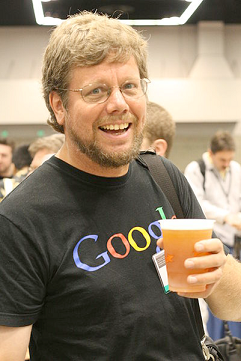
\includegraphics[width=0.8\linewidth,keepaspectratio]{rossum}
\end{center}
\tiny{(Reference: https://en.wikipedia.org/ wiki/Guido\_van\_Rossum)}
\end{minipage}
}
\end{frame}



%%%%%%%%%%%%%%%%%%%%%%%%%%%%%%%%%%%%%%%%%%%%%%%%%%%%%%%%%%%%%%%%%%%%%%%%%%%%%%%%%%%
\begin{frame}[fragile]  \frametitle{What is Python?}
\begin{itemize}
\item Interpreted
\item Object-oriented 
\item High-level
\item Dynamic semantics
\item Cross-platform
\item Readability.
\end{itemize}


\end{frame}


%%%%%%%%%%%%%%%%%%%%%%%%%%%%%%%%%%%%%%%%%%%%%%%%%%%%%%%%%%%%%%%%%%%%%%%%%%%%%%%%%%%
\begin{frame}[fragile]  \frametitle{Compiled Languages}
\begin{itemize}
\item Needs entire program
\item Translates directly to machine codes 
\item Exe native and fast
\item Usually statically typed
\item Types known during compilation
\item Change in type : recompilation
\item Ideal for compute-heavy tasks
\item E.g. C, C++, FORTRAN
\end{itemize}
\end{frame}

%%%%%%%%%%%%%%%%%%%%%%%%%%%%%%%%%%%%%%%%%%%%%%%%%%%%%%%%%%%%%%%%%%%%%%%%%%%%%%%%%%%
\begin{frame}[fragile]  \frametitle{Interpreted Languages}
\begin{itemize}
\item  Interpreted on the fly
\item No need to compile: can execute right away
\item Usually dynamically typed
\item Non-syntax errors are detected only in run-time
\item Slower than compiled languages
\item Ideal for small tasks
\item  E.g. Python, Perl, PHP, Bash
\end{itemize}

Note: Python, at the beginning, loosely checks the program. Only at run time, line-by-line, it checks for errors. So, if the error statements are not in the running path, their error does not get reported. So, its a bit relaxed. Thats the objection for its use in production code, where strong type checking and error checking, upfront is essential.
\end{frame}

%%%%%%%%%%%%%%%%%%%%%%%%%%%%%%%%%%%%%%%%%%%%%%%%%%%%%%%%%%%%%%%%%%%%%%%%%%%%%%%%%%%
\begin{frame}[fragile]  \frametitle{JIT-Compiled Languages}
\begin{itemize}
\item Between compiled and interpreted
\item Code is initially interpreted, hotspots compiled
\item Deduce types during compilation, can change in run-time
\item Slower than compiled
\item E.g. Java, C\#
\end{itemize}
\end{frame}

%%%%%%%%%%%%%%%%%%%%%%%%%%%%%%%%%%%%%%%%%%%%%%%%%%%%%%%%%%%%%%%%%%%%%%%%%%%%%%%%%%%
\begin{frame}[fragile]  \frametitle{``C'' guys to take pride in}
\begin{itemize}
\item Python interpreter written in  ``C''
\item Source code at www.python.org
\item So, Python Interpreter is compiled exe
%\item On windows, its \lstinline|C:\Python35\python.exe|
\end{itemize}
\end{frame}


%%%%%%%%%%%%%%%%%%%%%%%%%%%%%%%%%%%%%%%%%%%%%%%%%%%%%%%%%%%%%%%%%%%%%%%%%%%%%%%%%%%
\begin{frame}[fragile]  \frametitle{Completely Controversial Observations about Languages}
\begin{center}
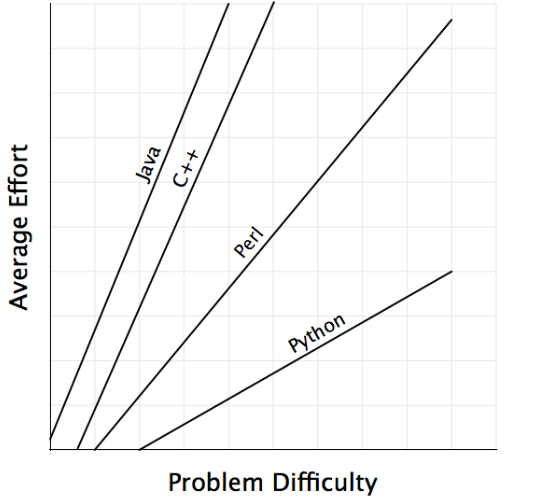
\includegraphics[width=0.6\linewidth,keepaspectratio]{langs}
\end{center}
\end{frame}


%%%%%%%%%%%%%%%%%%%%%%%%%%%%%%%%%%%%%%%%%%%%%%%%%%%%%%%%%%%%%%%%%%%%%%%%%%%%%%%%%%%
\begin{frame}[fragile]  \frametitle{Python Help}
\begin{itemize}
\item Home page -- http://www.python.org
\item Wiki -- http://wiki.python.org/
\item  Packages -- https://pypi.python.org/pypi
\item Projects at http://sourceforge.net and github.org
%\item Import a module, then view its  \lstinline{.__doc__}  attribute.
%\item At the interactive prompt, use  \lstinline{help(obj)}
\end{itemize}
\end{frame}


%%%%%%%%%%%%%%%%%%%%%%%%%%%%%%%%%%%%%%%%%%%%%%%%%%%%%%%%%%%%%%%%%%%%%%%%%%%%%%%%%%%
\begin{frame}[fragile]  \frametitle{Important features}
\begin{itemize}
\item Built-in high level data types: \lstinline{strings, lists, dictionaries}, etc.
\item Usual control structures: \lstinline{if, if-else, if-elif-else, while, for}
\item Levels of organization: \lstinline{functions, classes, modules, packages}
\item Extensions in C and C++ possible
\end{itemize}
\end{frame}

%%%%%%%%%%%%%%%%%%%%%%%%%%%%%%%%%%%%%%%%%%%%%%%%%%%%%%%%%%%%%%%%%%%%%%%%%%%%%%%%%%%
\begin{frame}[fragile]  \frametitle{Python 2 \emph{vs} Python 3}
\begin{itemize}
\item Two major versions 2.*, 3.*
\item Python 2.7: Latest release in 2.x series
\item Python 3.5: More polished syntax, removed inconsistencies
\end{itemize}
\end{frame}

%%%%%%%%%%%%%%%%%%%%%%%%%%%%%%%%%%%%%%%%%%%%%%%%%%%%%%%%%%%%%%%%%%%%%%%%%%%%%%%%%%
\begin{frame}[fragile]\frametitle{}
\begin{center}
{\Large Installations}
\end{center}
\end{frame}

%%%%%%%%%%%%%%%%%%%%%%%%%%%%%%%%%%%%%%%%%%%%%%%%%%%%%%%%%%%%%%%%%%%%%%%%%%%%%%%%%%%
\begin{frame}[fragile]\frametitle{Installing Python}
  \begin{itemize}
  \item Pre-installed on most Unix, Linux and MAC OS X
   \item Windows: Python.org or Anaconda (preferred)
   \item Anaconda has necessary libraries
\item 2.* and 3.* both
\item `pip' and `conda'
  \end{itemize}
\end{frame}

%%%%%%%%%%%%%%%%%%%%%%%%%%%%%%%%%%%%%%%%%%%%%%%%%%%%%%%%%%%%%%%%%%%%%%%%%%%%%%%%%%%
\begin{frame}[fragile]\frametitle{Installing Python by Anaconda Distribution}
  \begin{itemize}
  \item Need Python 3.5 (not 2.* or 3.6)
  \item By default in Anaconda 4.2.0
  \item Site: https://repo.continuum.io/archive/
  \item 64 Bit: Anaconda3-4.2.0-Windows-x86\_64.exe
  \item 32 bit: Anaconda3-4.2.0-Windows-x86.exe
  \item About 300+MB
  \end{itemize}
\end{frame}

%%%%%%%%%%%%%%%%%%%%%%%%%%%%%%%%%%%%%%%%%%%%%%%%%%%%%%%%%%%%%%%%%%%%%%%%%%%%%%%%%%%
\begin{frame}[fragile]  \frametitle{The Python shell, I}
  \begin{itemize}
 \item Can run from ``shell'', IDE, Notebook
 \item Shell/Command Line:
\begin{lstlisting}
$ python

Python 3.5.3 | packaged by conda-forge | (default, May 12 2017, 16:16:49) [MSC v.1900 64 bit (AMD64)] on win32
Type "help", "copyright", "credits" or "license" for more information.
>>>
\end{lstlisting}
\item Start typing at  $>>>$ 
\end{itemize}
\end{frame}

%%%%%%%%%%%%%%%%%%%%%%%%%%%%%%%%%%%%%%%%%%%%%%%%%%%%%%%%%%%%%%%%%%%%%%%%%%%%%%%%%%%
\begin{frame}[fragile]  \frametitle{The Python shell, I}
  \begin{itemize}
 \item Typing anything??
\begin{lstlisting}
>>> I come in peace, please take me to your leader
File "<stdin>" , line 1
I come in peace, please take me to your leader
^
SyntaxError : invalid syntax
>>>
\end{lstlisting}
\item Need to learn syntax
\end{itemize}
\end{frame}

%%%%%%%%%%%%%%%%%%%%%%%%%%%%%%%%%%%%%%%%%%%%%%%%%%%%%%%%%%%%%%%%%%%%%%%%%%%%%%%%%%%
\begin{frame}[fragile]\frametitle{The Python shell, II}
\begin{itemize}
\item Expressions: evaluated, result printed:
\begin{lstlisting}
>>> 2+2
4
\end{lstlisting}
\item Line continuation \\ 
\begin{lstlisting}
>>> "hello" + \
... " world!"
'hello world!'
\end{lstlisting}
\item Prompt changes to `\texttt{...}' on continuation lines.
\end{itemize}
\end{frame}

%%%%%%%%%%%%%%%%%%%%%%%%%%%%%%%%%%%%%%%%%%%%%%%%%%%%%%%%%%%%%%%%%%%%%%%%%%%%%%%%%%%
\begin{frame}[fragile]\frametitle{The Python shell, II}
\begin{itemize}
\item Syntactically correct:
	\begin{lstlisting}
>>>print('I come in peace, please take me')
	\end{lstlisting}

\item \lstinline|print| is a function, with defined syntax. 
\item If you don't obey: \\ 
\begin{lstlisting}
>>>print 'I come in peace, please take me'
File "<stdin>", line 1
print 'I come in peace, please take me'
^
SyntaxError: Missing parentheses in call to 'print'
\end{lstlisting}
\end{itemize}
\end{frame}

%%%%%%%%%%%%%%%%%%%%%%%%%%%%%%%%%%%%%%%%%%%%%%%%%%%%%%%%%%%%%%%%%%%%%%%%%%%%%%%%%%%
\begin{frame}[fragile]\frametitle{The Python shell, II}
\begin{itemize}
\item To exit:
	\begin{lstlisting}
>>> good-bye
Traceback (most recent call last):
File"<stdin>", line1, in <module>
NameError name 'good' is not defined
>>> if you don't mind, I need to leave 
File "<stdin>", line 1
if you don't mind, I need to leave
          ^
SyntaxError: invalid syntax
	\end{lstlisting}

\item Better to: \\ 
\begin{lstlisting}
>>> quit()
\end{lstlisting}
\end{itemize}
\end{frame}

%%%%%%%%%%%%%%%%%%%%%%%%%%%%%%%%%%%%%%%%%%%%%%%%%%%%%%%%%%%%%%%%%%%%%%%%%%%%%%%%%%%
\begin{frame}[fragile]\frametitle{Exercises}
\begin{itemize}
\item Find more about JIT-compilation.
\item Install any IDE, having debugging.
\item Get familiar with command prompt.
\end{itemize}
\end{frame}

%%%%%%%%%%%%%%%%%%%%%%%%%%%%%%%%%%%%%%%%%%%%%%%%%%%%%%%%%%%%%%%%%%%%%%%%%%%%%%%%%%%
\begin{frame}[fragile]\frametitle{Integrated Dev Envt}
  \begin{itemize}
  \item Pycharm https://www.jetbrains.com/pycharm/
  \item IDLE comes with python.org distribution
  \item Spyder https://pypi.python.org/pypi/spyder
  \end{itemize}
\end{frame}

%%%%%%%%%%%%%%%%%%%%%%%%%%%%%%%%%%%%%%%%%%%%%%%%%%%%%%%%%%%%%%%%%%%%%%%%%%%%%%%%%%%
\begin{frame}[fragile]\frametitle{PyCharm}
Download the community edition of Pycharm
\begin{center}
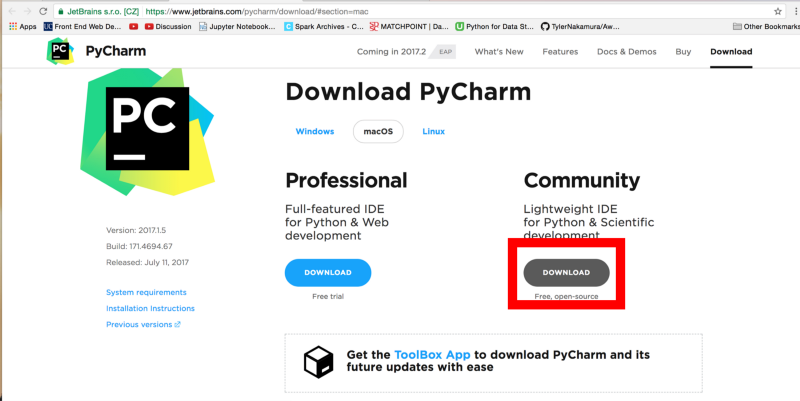
\includegraphics[width=0.7\linewidth,keepaspectratio]{pycharm1}
\end{center}
\end{frame}

%%%%%%%%%%%%%%%%%%%%%%%%%%%%%%%%%%%%%%%%%%%%%%%%%%%%%%%%%%%%%%%%%%%%%%%%%%%%%%%%%%%
\begin{frame}[fragile]\frametitle{PyCharm Project}
Create a New Project
\begin{center}
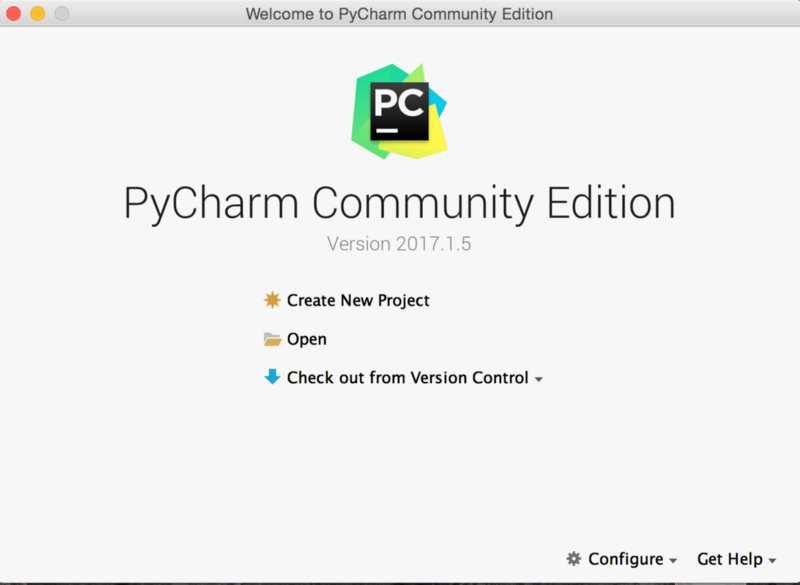
\includegraphics[width=0.7\linewidth,keepaspectratio]{pycharm2}
\end{center}
\end{frame}

%%%%%%%%%%%%%%%%%%%%%%%%%%%%%%%%%%%%%%%%%%%%%%%%%%%%%%%%%%%%%%%%%%%%%%%%%%%%%%%%%%%
\begin{frame}[fragile]\frametitle{PyCharm Exercise}

  \begin{itemize}
  \item Create a directory.
  \item Create New Project in Pychram. 
  \item Give the newly created dir as path.
  \item Create New Python file. Write:
    \begin{lstlisting}
 print(``Hello World!!'')
    \end{lstlisting}
  \item Run.
  \item Result?.
  \item Get familiar with Pycharm UI.
  \end{itemize}
\end{frame}




\section[Basics]{Module 2: Basics}
%%%%%%%%%%%%%%%%%%%%%%%%%%%%%%%%%%%%%%%%%%%%%%%%%%%%%%%%%%%%%%%%%%%%%%%%%%%%%%%%%%
\begin{frame}[fragile]\frametitle{}
\begin{center}
{\Large Syntax}
\end{center}
\end{frame}

%%%%%%%%%%%%%%%%%%%%%%%%%%%%%%%%%%%%%%%%%%%%%%%%%%%%%%%%%%%%%%%%%%%%%%%%%%%%%%%%%%%
\begin{frame}[fragile] \frametitle{Lines}
\begin{itemize}
\item  Statement separator : a semi-colon, 
\item Only needed for multiple statements on a line. 
\item Else, nothing
\item Continuation: a back-slash
\item  But, not necessary in ``context'' : ( ),\{ \},[ ]
\end{itemize}
\end{frame}

%%%%%%%%%%%%%%%%%%%%%%%%%%%%%%%%%%%%%%%%%%%%%%%%%%%%%%%%%%%%%%%%%%%%%%%%%%%%%%%%%%%
\begin{frame}[fragile] \frametitle{Blocks and indentation}
\begin{itemize}
\item  Blocks by indentation
\item No begin/end brackets
\item Indentation is 4 spaces and no hard tabs
\item Reduces clutter
\item \lstinline{if, while, function, except}, etc have $:$ at the end
\item $:$ must follow with an indent on next line.
\end{itemize}
\end{frame}


%%%%%%%%%%%%%%%%%%%%%%%%%%%%%%%%%%%%%%%%%%%%%%%%%%%%%%%%%%%%%%%%%%%%%%%%%%%%%%%%%%%
\begin{frame}[fragile] \frametitle{Comments}
\begin{itemize}
\item  Everything after ``\#'' ignored.
\begin{lstlisting}
# compute the percentage of the hour that has elapsed
percentage = (minute * 100) / 60

percentage = (minute * 100) / 60 # percentage per hour
\end{lstlisting}
\item Useless/redundant:
\begin{lstlisting}
v = 5 # assign 5 to v
\end{lstlisting}
\item Useful info:
\begin{lstlisting}
v = 5 # velocity in meters/second.
\end{lstlisting}
\end{itemize}
\end{frame}

%%%%%%%%%%%%%%%%%%%%%%%%%%%%%%%%%%%%%%%%%%%%%%%%%%%%%%%%%%%%%%%%%%%%%%%%%%%%%%%%%%%
\begin{frame}[fragile] \frametitle{Comments}
No block comments
\begin{lstlisting}
# A comment, this is so you can read program later.
# Anything after the # is ignored by python.
print("something.") # and the comment after is ignored

# Use a comment to "disable" a piece of code:
# print("This won't run.")
print("This will run.")
\end{lstlisting}

\end{frame}


% %%%%%%%%%%%%%%%%%%%%%%%%%%%%%%%%%%%%%%%%%%%%%%%%%%%%%%%%%%%%%%%%%%%%%%%%%%%%%%%%%%%
% \begin{frame}[fragile] \frametitle{Doc strings}
% Doc strings: Comments in quotes at start of module, class, method or function.
% \begin{lstlisting}
% """and here....

% I hate Python
% Nah, just kidding...

% is a multi-line comment"""
% def myfunc():
    % pass
% \end{lstlisting}
% By triple-quoting spanning multiple lines.
% \end{frame}


% %%%%%%%%%%%%%%%%%%%%%%%%%%%%%%%%%%%%%%%%%%%%%%%%%%%%%%%%%%%%%%%%%%%%%%%%%%%%%%%%%%%
% \begin{frame}[fragile] \frametitle{Doc strings}
% \begin{itemize}
% \item  Carried with executing code. 
% \item Viewed with  \lstinline|help() ,  obj.__doc__ |
% \item IPython: Question mark ( ? ) after, for help.

% \end{itemize}
% \end{frame}

% %%%%%%%%%%%%%%%%%%%%%%%%%%%%%%%%%%%%%%%%%%%%%%%%%%%%%%%%%%%%%%%%%%%%%%%%%%%%%%%%%%%
% \begin{frame}[fragile]\frametitle{Exercise}
% \begin{itemize}
% \item  Python has many built-in functions, and if you do not know how to use it, you can read document online or find some books. But Python has a built-in document function for every built-in functions.
% \item      Please write a program to print some Python built-in functions documents, such as abs(), int(), raw\_input()
% \item      And add document for your own function
    
% \item  Hints:     The built-in document method is \_\_doc\_\_
% \end{itemize}
% \end{frame}

% %%%%%%%%%%%%%%%%%%%%%%%%%%%%%%%%%%%%%%%%%%%%%%%%%%%%%%%%%%%%%%%%%%%%%%%%%%%%%%%%%%%
% \begin{frame}[fragile]\frametitle{Solution}
% \begin{lstlisting}
% print(abs.__doc__)
% print(int.__doc__)
% print)input.__doc__)

% def square(num):
    % '''Return the square value of the input number.
    
    % The input number must be integer.
    % '''
    % return num ** 2

% print(square(2))
% print(square.__doc__)
% \end{lstlisting}
% \end{frame}

% %%%%%%%%%%%%%%%%%%%%%%%%%%%%%%%%%%%%%%%%%%%%%%%%%%%%%%%%%%%%%%%%%%%%%%%%%%%%%%%%%%%
% \begin{frame}[fragile] \frametitle{Program structure}
% \begin{itemize}
% \item  \lstinline|def, class| add something to current name-space. 
% \item Modules: both executable and import-able.
% \item Modules: correspond to files with ``*.py''. 
% \item Packages: correspond to directory, importable
% \item A package contains \lstinline|__init__.py|. 
% \end{itemize}
% \end{frame}




%%%%%%%%%%%%%%%%%%%%%%%%%%%%%%%%%%%%%%%%%%%%%%%%%%%%%%%%%%%%%%%%%%%%%%%%%%%%%%%%%%
\begin{frame}[fragile]\frametitle{}
\begin{center}
{\Large Data Types}
\end{center}
\end{frame}

%%%%%%%%%%%%%%%%%%%%%%%%%%%%%%%%%%%%%%%%%%%%%%%%%%%%%%%%%%%%%%%%%%%%%%%%%%%%%%%%%%%
\begin{frame}[fragile]\frametitle{Variables}

  \begin{itemize}
  \item A variable can be seen as a container (or some say a pigeonhole) to store certain values. 
  \item While the program is running, variables are accessed and sometimes changed, i.e. a new value will be assigned to a variable. 
    \item Every variable has and must have a unique data type.
  \item Declaring a variable means binding it to a data type.
  \item Defining a variable meas to have value assigned to it.
    \end{itemize}

\end{frame}

%%%%%%%%%%%%%%%%%%%%%%%%%%%%%%%%%%%%%%%%%%%%%%%%%%%%%%%%%%%%%%%%%%%%%%%%%%%%%%%%%%%
\begin{frame}[fragile]\frametitle{Variables in C/C++ or Java}
  \begin{columns}[c]
    \begin{column}{0.5\linewidth}
  \begin{lstlisting}
int x;
int y; 
\end{lstlisting}
  \begin{itemize}
  \item Such declarations make sure that the program reserves memory for two variables with the names x and y. 
  \item The variable names stand for the memory location. 
  \item It's like the two empty shoeboxes, labelled with x and y. 
  \item Like the two shoeboxes, the memory is empty as well.
    \end{itemize}
      \end{column}
    \begin{column}{0.4\linewidth}
    \begin{center}
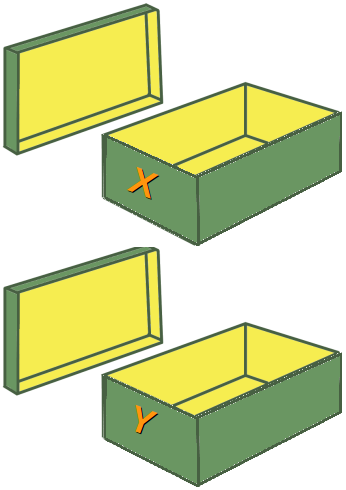
\includegraphics[width=0.3\linewidth,keepaspectratio]{boxes1}
\end{center}
        \end{column}
  \end{columns}
  
   % (Ref: https://www.python-course.eu/python3\_variables.php)
\end{frame}

%%%%%%%%%%%%%%%%%%%%%%%%%%%%%%%%%%%%%%%%%%%%%%%%%%%%%%%%%%%%%%%%%%%%%%%%%%%%%%%%%%%
\begin{frame}[fragile]\frametitle{Variables in C/C++ or Java}
  \begin{columns}[c]
    \begin{column}{0.5\linewidth}
  \begin{lstlisting}
x = 42;
y = 42; 
\end{lstlisting}
  \begin{itemize}
  \item Putting values into the variables can be realized with assignments. 
  \item Two numbers are physically saved in the memory, which correspond to the two shoeboxes.
    \end{itemize}
      \end{column}
    \begin{column}{0.4\linewidth}
    \begin{center}
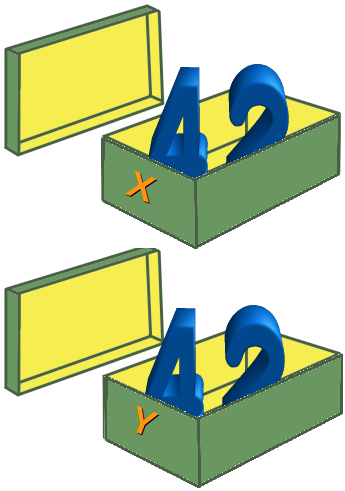
\includegraphics[width=0.3\linewidth,keepaspectratio]{boxes2}
\end{center}
        \end{column}
  \end{columns}
  
   % (Ref: https://www.python-course.eu/python3\_variables.php)
\end{frame}


%%%%%%%%%%%%%%%%%%%%%%%%%%%%%%%%%%%%%%%%%%%%%%%%%%%%%%%%%%%%%%%%%%%%%%%%%%%%%%%%%%%
\begin{frame}[fragile]\frametitle{Variables in C/C++ or Java}
  \begin{columns}[c]
    \begin{column}{0.5\linewidth}
  \begin{lstlisting}
y = 78;
\end{lstlisting}
  \begin{itemize}
  \item If we assign a new value to one of the variables, let's say the values 78 to y.
  \item We have exchanged the content of the memory location of y.

    \end{itemize}
      \end{column}
    \begin{column}{0.4\linewidth}
    \begin{center}
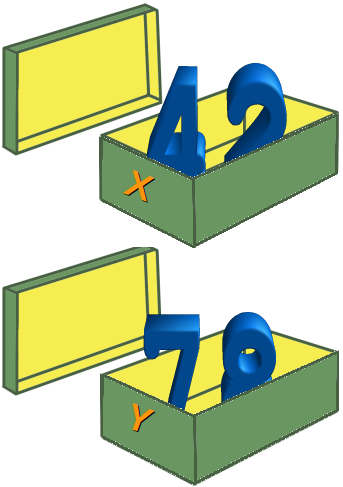
\includegraphics[width=0.3\linewidth,keepaspectratio]{boxes3}
\end{center}
        \end{column}
  \end{columns}
  
   % (Ref: https://www.python-course.eu/python3\_variables.php)
\end{frame}

%%%%%%%%%%%%%%%%%%%%%%%%%%%%%%%%%%%%%%%%%%%%%%%%%%%%%%%%%%%%%%%%%%%%%%%%%%%%%%%%%%%
\begin{frame}[fragile]\frametitle{Variables in Python}

  \begin{itemize}
  \item There is no declaration of variables required.
  \item Not only the value of a variable may change during program execution but the type as well.
\item You can assign an integer value to a variable, use it as an integer for a while and then assign a string to the same variable. 
    \end{itemize}

  \begin{lstlisting}
i = 42			# data type is implicitly set to integer
i = 42 + 0.11		# data type is changed to float
i = "forty"		# and now it will be a string  
\end{lstlisting}
  
   % (Ref: https://www.python-course.eu/python3\_variables.php)
\end{frame}


%%%%%%%%%%%%%%%%%%%%%%%%%%%%%%%%%%%%%%%%%%%%%%%%%%%%%%%%%%%%%%%%%%%%%%%%%%%%%%%%%%%
\begin{frame}[fragile]\frametitle{All variables in Python are references}
Python variables are references to objects, but the actual data is contained in the objects: 

    \begin{center}
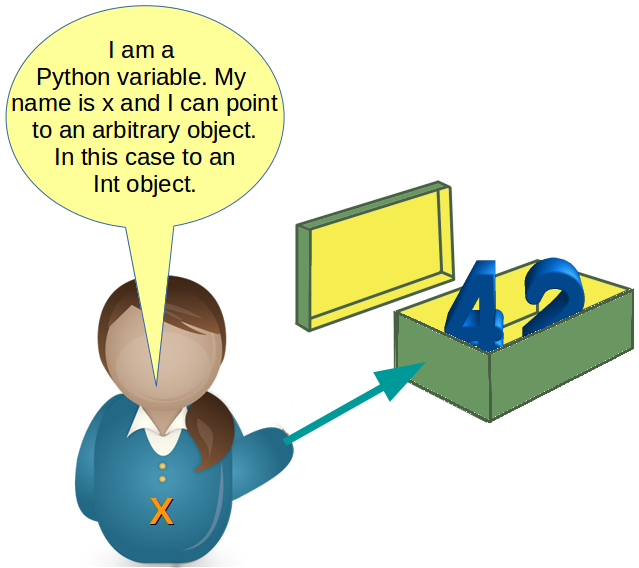
\includegraphics[width=0.5\linewidth,keepaspectratio]{boxes4}
\end{center}
  
  As variables are pointing to objects and objects can be of arbitrary data type, variables cannot have types associated with them.
  
   % (Ref: https://www.python-course.eu/python3\_variables.php)
   
   
\end{frame}


%%%%%%%%%%%%%%%%%%%%%%%%%%%%%%%%%%%%%%%%%%%%%%%%%%%%%%%%%%%%%%%%%%%%%%%%%%%%%%%%%%%
\begin{frame}[fragile]\frametitle{All variables are references}
\begin{lstlisting}
>>> x = 42
>>> y = x
\end{lstlisting}



    \begin{center}
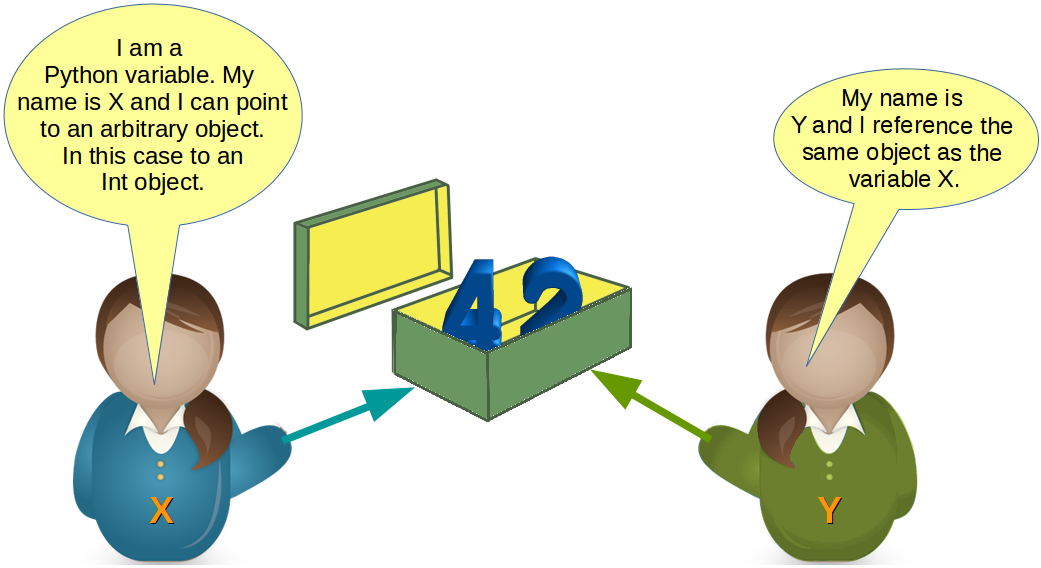
\includegraphics[width=0.5\linewidth,keepaspectratio]{boxes5}
\end{center}
  
  
   % (Ref: https://www.python-course.eu/python3\_variables.php)
   
   
\end{frame}



%%%%%%%%%%%%%%%%%%%%%%%%%%%%%%%%%%%%%%%%%%%%%%%%%%%%%%%%%%%%%%%%%%%%%%%%%%%%%%%%%%%
\begin{frame}[fragile]\frametitle{All variables are references}

What will happen, when we execute 

\begin{lstlisting}
y = 78
\end{lstlisting}
Python will create a new integer object with the content 78 and then the variable y will reference this newly created object, as we can see in the following picture: 


    \begin{center}
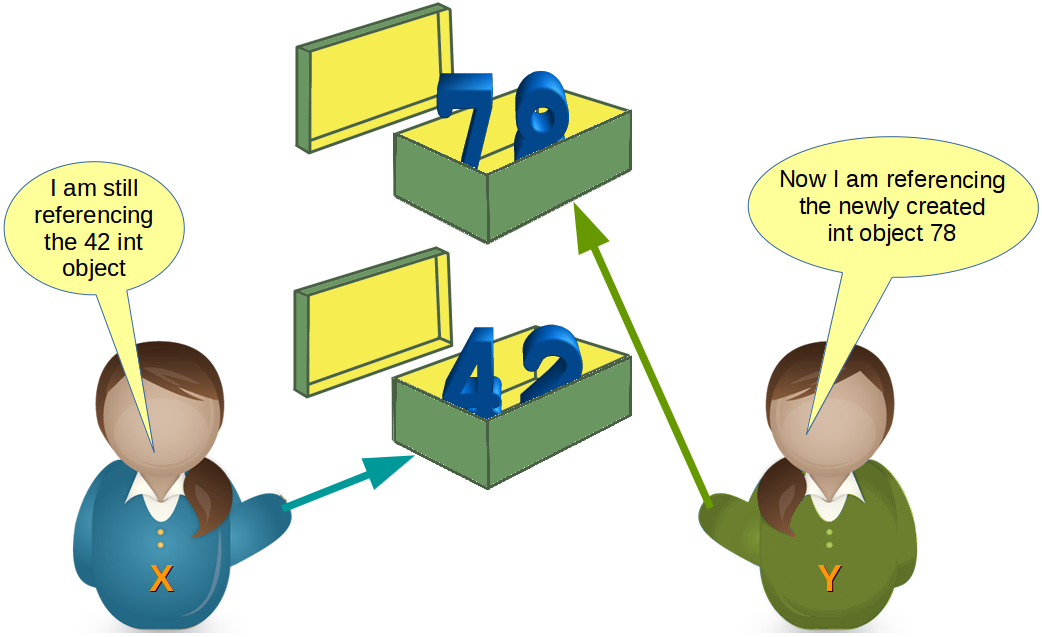
\includegraphics[width=0.5\linewidth,keepaspectratio]{boxes6}
\end{center}
  
  
   % (Ref: https://www.python-course.eu/python3\_variables.php)
   
   
\end{frame}


%%%%%%%%%%%%%%%%%%%%%%%%%%%%%%%%%%%%%%%%%%%%%%%%%%%%%%%%%%%%%%%%%%%%%%%%%%%%%%%%%%%
\begin{frame}[fragile]\frametitle{All variables are references}

What will happen, when we execute 

\begin{lstlisting}
x = ``Text''
\end{lstlisting}
The previously integer object "42" will be orphaned after this assignment. It will be removed by Python, because no other variable is referencing it. 


    \begin{center}
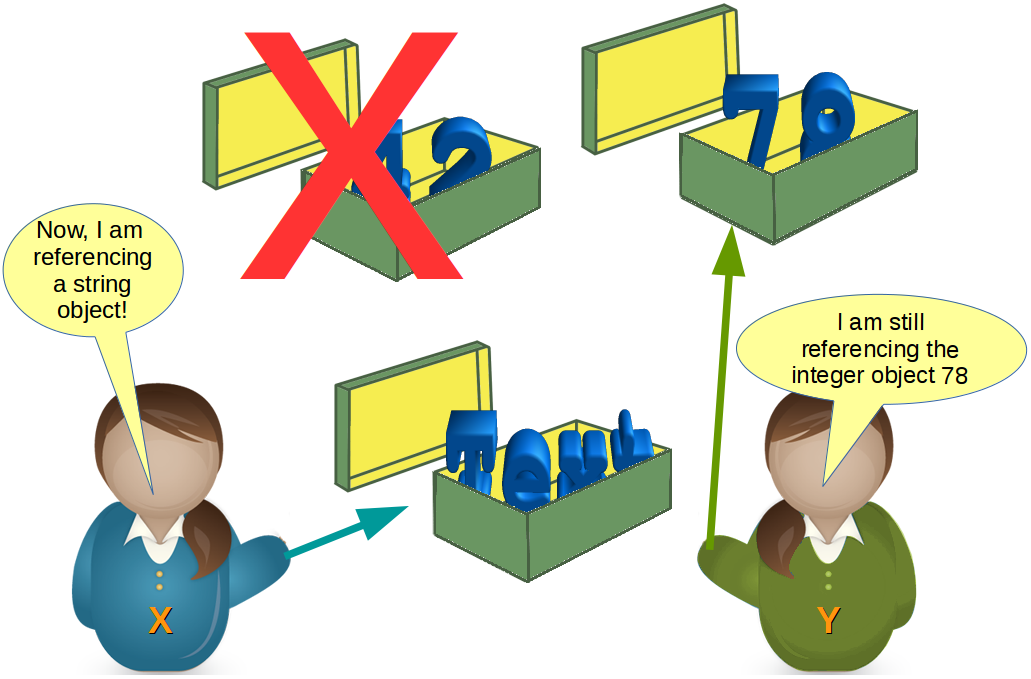
\includegraphics[width=0.5\linewidth,keepaspectratio]{boxes7}
\end{center}
  
  
   % (Ref: https://www.python-course.eu/python3\_variables.php)
   
   
\end{frame}


%%%%%%%%%%%%%%%%%%%%%%%%%%%%%%%%%%%%%%%%%%%%%%%%%%%%%%%%%%%%%%%%%%%%%%%%%%%%%%%%%%%
\begin{frame}[fragile]\frametitle{All variables are references}
In Python, \textbf{all objects are ever passed by reference}.
In particular, \textbf{variables always store a reference to an
    object}, never a copy!

  
  Hence, you have to be careful when modifying objects:
\begin{lstlisting}
>>> a = [1,2,3]
>>> b = a
>>> b.remove(2)
>>> print(a)
\end{lstlisting}

\emph{???}

\textbf{Q}: How many items are in the \texttt{a} list now?
%[1, 3]
\end{frame}


%%%%%%%%%%%%%%%%%%%%%%%%%%%%%%%%%%%%%%%%%%%%%%%%%%%%%%%%%%%%%%%%%%

 \begin{frame}[fragile]
   \frametitle{All variables are references}
   
However

 \begin{lstlisting}
 >>> a = 1
 >>> b = a
 >>> b += 1
 >>> a
 1
 >>> b
 2
 \end{lstlisting}

     How can you explain this?

     The $b += 1$ operator could be replaced by    $b = b + 1$, and the $b+1$ expression yields a
       new value.

 \end{frame}


%%%%%%%%%%%%%%%%%%%%%%%%%%%%%%%%%%%%%%%%%%%%%%%%%%%%%%%%%%%%%%%%%%%%%%%%%%%%%%%%%%%
\begin{frame}[fragile]\frametitle{Dynamic Typing: Python}
  \begin{itemize}
  \item Variables come into existence at first assignment.
  \item A variable can refer to an object of any type.
\item Can switch type based on assignment
  \item All types (almost) treated the same way.
  \item Type errors only caught in runtime.
    \end{itemize}

\end{frame}


%%%%%%%%%%%%%%%%%%%%%%%%%%%%%%%%%%%%%%%%%%%%%%%%%%%%%%%%%%%%%%%%%%%%%%%%%%%%%%%%%%%
\begin{frame}[fragile]\frametitle{Variables}
Definition-Declaration?
\begin{itemize}
\item  Assignment: Definition + Declaration:
\begin{lstlisting}
>>> n = 17

>>> pi = 3.1415926535897931

>>> message = 'And now for something different'
\end{lstlisting}
\end{itemize}
\end{frame}

%%%%%%%%%%%%%%%%%%%%%%%%%%%%%%%%%%%%%%%%%%%%%%%%%%%%%%%%%%%%%%%%%%%%%%%%%%%%%%%%%%%
\begin{frame}[fragile]\frametitle{Variables Value}
\begin{itemize}
\item Display value
\begin{lstlisting}
>>> print(n)
17

>>> print(pi)
3.141592653589793

>>> print(message)
???
\end{lstlisting}
\end{itemize}
\end{frame}


%%%%%%%%%%%%%%%%%%%%%%%%%%%%%%%%%%%%%%%%%%%%%%%%%%%%%%%%%%%%%%%%%%%%%%%%%%%%%%%%%%%
\begin{frame}[fragile]\frametitle{Variables Type}
\begin{itemize}
\item Display type
\begin{lstlisting}
>>> print(type(n))
<class 'int'>

>>> print(type(pi))
<class 'float'>

>>> print(type(message))
??
\end{lstlisting}
\end{itemize}
\end{frame}



% %%%%%%%%%%%%%%%%%%%%%%%%%%%%%%%%%%%%%%%%%%%%%%%%%%%%%%%%%%%%%%%%%%%%%%%%%%%%%%%%%%%
% \begin{frame}[fragile]\frametitle{Mutability}
% \begin{itemize}
% \item Data types : mutable or immutable. 
% \item The content of objects of immutable types cannot be changed after they are created.
% \item Immutable: int, float, complex, str, tuple, frozenset, bool
% \item Mutable: list, set, dict
% \item Only mutable objects support methods that change the object in place, such as reassignment of a sequence slice, which will work for lists, but raise an error for tuples and strings.
% \end{itemize}

% (Ref: https://en.wikibooks.org/wiki/Python\_Programming/Data\_Types\#Mutable\_vs\_Immutable\_Objects)
% \end{frame}


% %%%%%%%%%%%%%%%%%%%%%%%%%%%%%%%%%%%%%%%%%%%%%%%%%%%%%%%%%%%%%%%%%%%%%%%%%%%%%%%%%%%
% \begin{frame}[fragile]\frametitle{Mutability}
% \begin{itemize}
% \item Variables in Python are really just references to objects in memory. 
% \item If you assign an object to a variable as below
% \begin{lstlisting}
% a = 1
% s = 'abc'
% l = ['a string', 456]
% \end{lstlisting}
% \item All you really do is make this variable a, s, l point to the objects 1, 'abc',  ['a string', 456] respectively.
% \item If you reassign a variable as below
% \begin{lstlisting}
% a = 7
% s = 'xyz'
% l = ['a simpler list', 99, 10]
% \end{lstlisting}
% \item You make the variable point to a different object 
% \item Use id(x) method to confirm the ids before/after the assignment.
% \end{itemize}
% \end{frame}

% %%%%%%%%%%%%%%%%%%%%%%%%%%%%%%%%%%%%%%%%%%%%%%%%%%%%%%%%%%%%%%%%%%%%%%%%%%%%%%%%%%%
% \begin{frame}[fragile]\frametitle{Mutability}
% \begin{itemize}
% \item Only mutable objects can be changed in place (l[0] = 1 is ok in our example, but s[0] = 'a' raises an error). 
% \item Tricky when it happens silently in += operator
% \begin{lstlisting}
% a += 1
% s += 'qwertz'
% \end{lstlisting}
% \item Python will silently create a new object and make the variable point to it. 
% However, when used on a mutable object, the object pointed to by the variable will be changed in place. 
% \begin{lstlisting}
% l += [1,2,3]
% \end{lstlisting}
% \item You make the variable point to a different object 
% \item Use id(x) method to confirm the ids before/after the assignment.
% \end{itemize}
% \end{frame}

% %%%%%%%%%%%%%%%%%%%%%%%%%%%%%%%%%%%%%%%%%%%%%%%%%%%%%%%%%%%%%%%%%%%%%%%%%%%%%%%%%%%
% \begin{frame}[fragile]\frametitle{Mutability}
% \begin{itemize}
% \item Assume
% \begin{lstlisting}
% p = s
% m = l
% s += 'etc'
% l += [9,8,7].
% \end{lstlisting}
% \item This will change s and leave p unaffected, but will change both m and l since both point to the same list object. 
% \item Python's built-in id() function, which returns a unique object identifier for a given variable name, can be used to trace what is happening under the hood.
% \end{itemize}
% \end{frame}


%%%%%%%%%%%%%%%%%%%%%%%%%%%%%%%%%%%%%%%%%%%%%%%%%%%%%%%%%%%%%%%%%%%%%%%%%%%%%%%%%%%
\begin{frame}[fragile]\frametitle{Variable Names}
\begin{itemize}
\item  Can be arbitrarily long. 
\item Can contain both letters and numbers, 
\item Cannot start with a number.
\item (\_) can appear in a name.
\item Reserves 33 keywords
\end{itemize}
\end{frame} 

%%%%%%%%%%%%%%%%%%%%%%%%%%%%%%%%%%%%%%%%%%%%%%%%%%%%%%%%%%%%%%%%%%%%%%%%%%%%%%%%%%%
\begin{frame}[fragile]\frametitle{Variable Names Errors}
\begin{lstlisting}
>>> 76trombones = 'big parade'
SyntaxError: invalid syntax

>>> more@ = 1000000
SyntaxError: invalid syntax

>>> class = 'Advanced Theoretical Zymurgy'
SyntaxError: invalid syntax
\end{lstlisting}
\end{frame} 
%%%%%%%%%%%%%%%%%%%%%%%%%%%%%%%%%%%%%%%%%%%%%%%%%%%%%%%%%%%%%%%%%%%%%%%%%%%%%%%%%%%
\begin{frame}[fragile]\frametitle{Choosing mnemonic variable names}
Variable names different but accomplishment same.
  \begin{itemize}
  \item 
\begin{lstlisting}
a = 35.0
b = 12.50
c = a * b
print(c)
\end{lstlisting}

\item

\begin{lstlisting}
hours = 35.0
rate = 12.50
pay = hours * rate
print(pay)
\end{lstlisting}

\item

\begin{lstlisting}
x1q3z9ahd = 35.0
x1q3z9afd = 12.50
x1q3p9afd = x1q3z9ahd * x1q3z9afd
print(x1q3p9afd)
\end{lstlisting}
  \end{itemize}
Which one better?
\end{frame} 

%%%%%%%%%%%%%%%%%%%%%%%%%%%%%%%%%%%%%%%%%%%%%%%%%%%%%%%%%%%%%%%%%%%%%%%%%%%%%%%%%%%
\begin{frame}[fragile]\frametitle{Basic Data types}
  \begin{itemize}
  \item {\bf bool} : \texttt{True}, \texttt{False}.
  \item {\bf int} Integer numbers.
  \item {\bf long}: Switches internally from \texttt{int} to \texttt{long} when needed.
  \item{\bf float} Double precision floating-point numbers
  \item {\bf str} String (bytes).
  %\item {\bf unicode} UNICODE String.
  \item{\bf list} Mutable list 
    \item{\bf tuple} Immutable list
        \item{\bf set} Unordered collection
  \item{\bf dict} Key/value mapping
  \end{itemize}
\end{frame}
%%%%%%%%%%%%%%%%%%%%%%%%%%%%%%%%%%%%%%%%%%%%%%%%%%%%%%%%%%%%%%%%%%%%%%%%%%%%%%%%%%%
\begin{frame}[fragile]\frametitle{Built-in object types}
  \begin{itemize}
  \item Numbers : \lstinline{3.1415, 1234, 999L, 3+4j}
  \item Strings : \lstinline{`spam', ``guido's''}
  \item Lists : \lstinline{[1, [2, `three'], 4]}
   \item Dictionaries :\lstinline|{`food':`spam', `taste':`yum'}|
  \item Tuples : \lstinline{(1,`spam', 4, `U')}
  \item Sets: \lstinline|{1,2,3,'foo','bar'}|
%  \item Files : \lstinline{text = open(`eggs', `r').read()}
  \end{itemize}
\end{frame}


%%%%%%%%%%%%%%%%%%%%%%%%%%%%%%%%%%%%%%%%%%%%%%%%%%%%%%%%%%%%%%%%%%%%%%%%%%%%%%%%%%%
\begin{frame}[fragile]\frametitle{Numbers}
  \begin{itemize}
  \item Integers : \lstinline{1234, -24, 0}
  \item Unlimited precision integers : \lstinline{ 999999999999L}
  \item Float : \lstinline{3.1415, 2.7122}
   \item Oct and hex :\lstinline|0177, 0x9ff|
  \item Complex : \lstinline{3+4j, 3.0+4.0j, 3J}
  \end{itemize}
\end{frame}




%%%%%%%%%%%%%%%%%%%%%%%%%%%%%%%%%%%%%%%%%%%%%%%%%%%%%%%%%%%%%%%%%%%%%%%%%%%%%%%%%%%
\begin{frame}[fragile]\frametitle{Integer}
\begin{lstlisting}
int_1 = 1
int_2 = -2
int_3 = 100

print(int_1 + int_2 + int_3) # for integers, + is  "plus"

# this is not what is looks like
print(1,000,000)

# eh, what is this then?
i = 1,000,000
type(i)

# Can I add these? Yes, but...
i = 1,000,000
j = 2,000,000
i + j

i / j
\end{lstlisting}
\end{frame}

%%%%%%%%%%%%%%%%%%%%%%%%%%%%%%%%%%%%%%%%%%%%%%%%%%%%%%%%%%%%%%%%%%%%%%%%%%%%%%%%%%%
\begin{frame}[fragile]\frametitle{Floating Point Numbers}
Decimal numbers, representations of fractions, "real-valued"
\begin{lstlisting}
float_1 = 1.2
float_2 = -4.0
float_3 = 10.0

print(float_1 + float_2 + float_3)

males = 7
females = 10
fraction = males/(males+females)
print("Percentage men: {}:".format(fraction))
\end{lstlisting}
\end{frame}

%%%%%%%%%%%%%%%%%%%%%%%%%%%%%%%%%%%%%%%%%%%%%%%%%%%%%%%%%%%%%%%%%%%%%%%%%%%%%%%%%%%
\begin{frame}[fragile]\frametitle{Booleans}
`True` or `False`.
\begin{lstlisting}
bool_1 = True 
bool_2 = False

print(bool_1)
print(bool_2)
\end{lstlisting}
\end{frame}

% %%%%%%%%%%%%%%%%%%%%%%%%%%%%%%%%%%%%%%%%%%%%%%%%%%%%%%%%%%%%%%%%%%%%%%%%%%%%%%%%%%%
% \begin{frame}[fragile]\frametitle{Exercise: Booleans}
% Can you become citizen? 
% You qualify if:
  % \begin{itemize}
  % \item Your parents are US Citizens and 
% \item You are under 18 or
% \item You have been born in the US
  % \end{itemize}
% \begin{lstlisting}
% age = 19
% parents_citizens = False 
% born_in_us = True

% citizen_eligible = False # Replace with an expression

% print("Citizen parents: {}; Age: {}; Born in US? {}\n Eligible for Citizen? {}".format(parents_citizens,age, born_in_us, citizen_eligible) )
% \end{lstlisting}
% \end{frame}


%%%%%%%%%%%%%%%%%%%%%%%%%%%%%%%%%%%%%%%%%%%%%%%%%%%%%%%%%%%%%%%%%%%%%%%%%%%%%%%%%%%
\begin{frame}[fragile]\frametitle{String Quotes}
\begin{itemize}
\item  Single and double quotes interchangeable:
\begin{lstlisting}
>>> "a string" == `a string'
True
\end{lstlisting}
\item One inside another ok:
\begin{lstlisting}
>>> a = "Isn't it ok?"
>>> b = `"Yes", he said.'
\end{lstlisting}
\item Just be consistent.
\end{itemize}
\end{frame}

%%%%%%%%%%%%%%%%%%%%%%%%%%%%%%%%%%%%%%%%%%%%%%%%%%%%%%%%%%%%%%%%%%%%%%%%%%%%%%%%%%%
\begin{frame}[fragile] \frametitle{Multi Line}
Multi-line strings with three quotes.
\begin{lstlisting}[showstringspaces=false]
str_10 = """
(CNN)AirAsia Flight QZ8501 climbed rapidly before it crashed, a top Indonesian official said Tuesday, according to The Jakarta Post. Then the plane stalled, Transportation Minister Ignasius Jonan said at a parliamentary hearing, according to the AFP and Reuters news agencies. "The plane, during the last minutes, went up faster than normal speed ... after then, it stalled. That is according to the data from the radar," Jonan said, according to the news agencies.
"""
print(str_10)
\end{lstlisting}
\end{frame}

%%%%%%%%%%%%%%%%%%%%%%%%%%%%%%%%%%%%%%%%%%%%%%%%%%%%%%%%%%%%%%%%%%%%%%%%%%%%%%%%%%%
\begin{frame}[fragile]\frametitle{String Indexing}
Can be indexed (subscripted), start at 0.
\begin{lstlisting}
word = 'Python'
word[0]  # character in position 0
word[1]
word[5]  # character in position 5
word[-1]  # last character
word[-2]  # second-last character
word[-6] #?
\end{lstlisting}
No separate character type:  a string of size one.
\end{frame}

%%%%%%%%%%%%%%%%%%%%%%%%%%%%%%%%%%%%%%%%%%%%%%%%%%%%%%%%%%%%%%%%%%%%%%%%%%%%%%%%%%%
\begin{frame}[fragile]\frametitle{Slicing}
\begin{lstlisting}
word[0:2]  # from position 0 (included) to 2 (excluded)
word[2:5]  # from position 2 (included) to 5 (excluded)
word[2:]  # from position 2 (included) to the end (excluded '\0')
word[:3]  # from beginning to position 3 (excluded)
word[-3:] # last three characters. 
word[-3:-1] # penultimate two characters
word[-1:-3] # Error. Wrong direction
Direction of substring is always from left to right.
\end{lstlisting}
\end{frame}

%%%%%%%%%%%%%%%%%%%%%%%%%%%%%%%%%%%%%%%%%%%%%%%%%%%%%%%%%%%%%%%%%%%%%%%%%%%%%%%%%%%
\begin{frame}[fragile]\frametitle{String Exercise}
  \begin{itemize}
  \item Assign the string 'Dealing with Data' to a Python variable.
  \item  Show usages positive indexing/slicing
  \item  Show usage of negative indexing/slicing
  \end{itemize}
\end{frame}



%%%%%%%%%%%%%%%%%%%%%%%%%%%%%%%%%%%%%%%%%%%%%%%%%%%%%%%%%%%%%%%%%%%%%%%%%%%%%%%%%%%
\begin{frame}[fragile]\frametitle{Start-End}
    Return \texttt{True} if \texttt{t} is the initial/final substring
  \begin{lstlisting}
  s.startswith(t)

  s.endswith(t)
  \end{lstlisting}
\end{frame}

%%%%%%%%%%%%%%%%%%%%%%%%%%%%%%%%%%%%%%%%%%%%%%%%%%%%%%%%%%%%%%%%%%%%%%%%%%%%%%%%%%%
\begin{frame}[fragile]\frametitle{String Exercise}
  \begin{itemize}
  \item Write a Python program to get a new string from a given string where ``Is'' has been added to the front. If the given string already begins with ``Is'' then return the string unchanged.
  \item  Write a Python program to get the n (non-negative integer) copies of the first 2 characters of a given string. Return the n copies of the whole string if the length is less than 2
  \end{itemize}
\end{frame}

%%%%%%%%%%%%%%%%%%%%%%%%%%%%%%%%%%%%%%%%%%%%%%%%%%%%%%%%%%%%%%%%%%%%%%%%%%%%%%%%%%%
\begin{frame}[fragile]\frametitle{Cases}
  \begin{lstlisting}
      s.capitalize() # First letter of sentence uppercase

      s.title() # First letter of all the words uppercase

      s.lower() # All letters lowercase

      s.upper()  # All letters uppercase
  \end{lstlisting}
    Copy of s is made, modified and returned.

\end{frame}

% %%%%%%%%%%%%%%%%%%%%%%%%%%%%%%%%%%%%%%%%%%%%%%%%%%%%%%%%%%%%%%%%%%%%%%%%%%%%%%%%%%%
% \begin{frame}[fragile]\frametitle{Exercise}
  % \begin{itemize}
  % \item Write a program that accepts a sentence and calculate the number of letters and digits.
  % \item Suppose the following input is supplied to the program: hello world! 123
  % \item Then, the output should be: LETTERS 10  DIGITS 3
  % \item Hints: In case of input data being supplied to the question, it should be assumed to be a console input.
  % \end{itemize}  
% \end{frame}

% %%%%%%%%%%%%%%%%%%%%%%%%%%%%%%%%%%%%%%%%%%%%%%%%%%%%%%%%%%%%%%%%%%%%%%%%%%%%%%%%%%%
% \begin{frame}[fragile]\frametitle{Solution}
  % \begin{lstlisting}
% s = input()
% d={"DIGITS":0, "LETTERS":0}
% for c in s:
    % if c.isdigit():
        % d["DIGITS"]+=1
    % elif c.isalpha():
        % d["LETTERS"]+=1
    % else:
        % pass
% print("LETTERS", d["LETTERS"])
% print("DIGITS", d["DIGITS"])
  % \end{lstlisting}
% \end{frame}

% %%%%%%%%%%%%%%%%%%%%%%%%%%%%%%%%%%%%%%%%%%%%%%%%%%%%%%%%%%%%%%%%%%%%%%%%%%%%%%%%%%%
% \begin{frame}[fragile]\frametitle{Exercise}
  % \begin{itemize}
  % \item Write a program that accepts sequence of lines as input and prints the lines after making all characters in the sentence capitalized.
  % \item Suppose the following input is supplied to the program: ``Hello world; Practice makes perfect''
  % \item Then, the output should be: ``HELLO WORLD; PRACTICE MAKES PERFECT''
  % \item Hints: In case of input data being supplied to the question, it should be assumed to be a console input.
  % \end{itemize}  
% \end{frame}

% %%%%%%%%%%%%%%%%%%%%%%%%%%%%%%%%%%%%%%%%%%%%%%%%%%%%%%%%%%%%%%%%%%%%%%%%%%%%%%%%%%%
% \begin{frame}[fragile]\frametitle{Solution}
  % \begin{lstlisting}
% lines = []
% while True:
    % s = input()
    % if s:
        % lines.append(s.upper())
    % else:
        % break;

% for sentence in lines:
    % print(sentence)
  % \end{lstlisting}
% \end{frame}



%%%%%%%%%%%%%%%%%%%%%%%%%%%%%%%%%%%%%%%%%%%%%%%%%%%%%%%%%%%%%%%%%%%%%%%%%%%%%%%%%%%
\begin{frame}[fragile]\frametitle{Split}
    Split \texttt{s} at every occurrence of \texttt{t} and return a list of parts. 
  \begin{lstlisting}
  	s.split(t)
  \end{lstlisting}
 If \texttt{t} is omitted, split on whitespace.
\end{frame}

%%%%%%%%%%%%%%%%%%%%%%%%%%%%%%%%%%%%%%%%%%%%%%%%%%%%%%%%%%%%%%%%%%%%%%%%%%%%%%%%%%%
\begin{frame}[fragile]\frametitle{Exercise}
  \begin{itemize}
  \item Write a program that computes the net amount of a bank account based a transaction log from console input. The transaction log format is shown as following:
    \begin{lstlisting}
D 100
W 200
  \end{lstlisting}
  \item D means deposit while W means withdrawal.
  \item Suppose the following input is supplied to the program:
    \begin{lstlisting}
D 300
D 300
W 200
D 100
  \end{lstlisting}
  \item Then, the output should be: 500
  \item  Hints:In case of input data being supplied to the question, it should be assumed to be a console input.
  \end{itemize}  
\end{frame}

%%%%%%%%%%%%%%%%%%%%%%%%%%%%%%%%%%%%%%%%%%%%%%%%%%%%%%%%%%%%%%%%%%%%%%%%%%%%%%%%%%%
\begin{frame}[fragile]\frametitle{Solution}
  \begin{lstlisting}
import sys
netAmount = 0
while True:
    s = input("Enter the transaction")
    if not s:
        break
    values = s.split(" ")
    operation = values[0]
    amount = int(values[1])
    if operation=="D":
        netAmount+=amount
    elif operation=="W":
        netAmount-=amount
    else:
        pass
print(netAmount)
  \end{lstlisting}
\end{frame}



%%%%%%%%%%%%%%%%%%%%%%%%%%%%%%%%%%%%%%%%%%%%%%%%%%%%%%%%%%%%%%%%%%%%%%%%%%%%%%%%%%%
\begin{frame}[fragile]\frametitle{Replace}
    Return a \emph{copy} of \texttt{s} with all \texttt{old} replaced by \texttt{new}.
  \begin{lstlisting}
  	s.replace(old, new)
  \end{lstlisting}
\end{frame}

%%%%%%%%%%%%%%%%%%%%%%%%%%%%%%%%%%%%%%%%%%%%%%%%%%%%%%%%%%%%%%%%%%%%%%%%%%%%%%%%%%%
\begin{frame}[fragile]\frametitle{Strip}
    Return a \emph{copy} of with the leading (resp.\ trailing, resp.\ leading \emph{and} trailing) whitespace removed.
  \begin{lstlisting}
      s.lstrip()

      s.rstrip()

      s.strip()
  \end{lstlisting}

\end{frame}


%%%%%%%%%%%%%%%%%%%%%%%%%%%%%%%%%%%%%%%%%%%%%%%%%%%%%%%%%%%%%%%%%%%%%%%%%%%%%%%%%%%
\begin{frame}[fragile]\frametitle{Finding text within string variables}
\begin{lstlisting}
word = "And on and on and on and on..." 
ind = word.find("on")
print(ind)
print("The first time on is at position", word.find("on"))

first_appearance = word.find("on")
second_appearance = word.find("on",first_appearance+1)
print("The second time on is at ", second_appearance)
\end{lstlisting}
\end{frame}


%%%%%%%%%%%%%%%%%%%%%%%%%%%%%%%%%%%%%%%%%%%%%%%%%%%%%%%%%%%%%%%%%%%%%%%%%%%%%%%%%%%
\begin{frame}[fragile]\frametitle{Finding text within string variables}
 Looking for "on" at the second half of "word"
\begin{lstlisting}
midpoint = int(len(word)/2) # finds middle of string word
second_half_appearance = word.find("on",midpoint)
print("First time 'on' in the second half: ", second_half_appearance)
\end{lstlisting}

\end{frame}


%%%%%%%%%%%%%%%%%%%%%%%%%%%%%%%%%%%%%%%%%%%%%%%%%%%%%%%%%%%%%%%%%%%%%%%%%%%%%%%%%%%
\begin{frame}[fragile]\frametitle{Finding text within string variables}
\begin{lstlisting}
word = "Python: And on and on and on and on..."
lookfor = "PYTHON"
count = word.count(lookfor)
print( "See '", lookfor  ,"' that many times: ",  count)
\end{lstlisting}
Exercise: Convert the code above to make it case-insensitive.
\end{frame}


%%%%%%%%%%%%%%%%%%%%%%%%%%%%%%%%%%%%%%%%%%%%%%%%%%%%%%%%%%%%%%%%%%%%%%%%%%%%%%%%%%%
\begin{frame}[fragile]\frametitle{Concatenating strings}
Old way:

\begin{lstlisting}
names = ['raymond', 'rachel', 'matthew', 'roger',
         'betty', 'melissa', 'judith', 'charlie']

s = names[0]
for name in names[1:]:
    s += ', ' + name
print(s)
\end{lstlisting}
Better:
\begin{lstlisting}
print ', '.join(names)
\end{lstlisting}


\tiny{(Ref: Transforming Code into Beautiful, Idiomatic Python -  Raymond Hettinger)}

\end{frame}


%%%%%%%%%%%%%%%%%%%%%%%%%%%%%%%%%%%%%%%%%%%%%%%%%%%%%%%%%%%%%%%%%%%%%%%%%%%%%%%%%%%
\begin{frame}[fragile]\frametitle{Joining list of Strings}
% print("practical data science".split(" "))
% print("hello".split(" "))
% print("practical data science".split("a"))

\begin{lstlisting}


mystring1 = "practical data science"
mylist1 = mystring1.split(" ")
print(mystring1)
print(mylist1)

" ".join(mylist1) # Try different "<c>" here
\end{lstlisting}
\end{frame}

%%%%%%%%%%%%%%%%%%%%%%%%%%%%%%%%%%%%%%%%%%%%%%%%%%%%%%%%%%%%%%%%%%%%%%%%%%%%%%%%%%%
\begin{frame}[fragile]\frametitle{String Comparisons}
\begin{lstlisting}
str_1 = "hello"
print("equality:")
print(str_1 == "hello")

print(str_1 == "Hello")
\end{lstlisting}
\end{frame}



% %%%%%%%%%%%%%%%%%%%%%%%%%%%%%%%%%%%%%%%%%%%%%%%%%%%%%%%%%%%%%%%%%%%%%%%%%%%%%%%%%%%
% \begin{frame}[fragile]\frametitle{String Comparisons}
% \begin{lstlisting}
% name1 = 'Abe'
% name2 = 'Bill'

% # Abe is lexicographically before Bill
% print(name1 < name2)

% \end{lstlisting}
% See ASCII table at http://www.asciitable.com/ for character order
% \end{frame}

% %%%%%%%%%%%%%%%%%%%%%%%%%%%%%%%%%%%%%%%%%%%%%%%%%%%%%%%%%%%%%%%%%%%%%%%%%%%%%%%%%%%
% \begin{frame}[fragile]\frametitle{String Comparisons}
% \begin{lstlisting}
% name1 = 'abe'
% name2 = 'Bill'
% # However 'abe' is lexicographically after Bill (which starts with an uppercase letter)
% print(name1 < name2)
% \end{lstlisting}

% \end{frame}

%%%%%%%%%%%%%%%%%%%%%%%%%%%%%%%%%%%%%%%%%%%%%%%%%%%%%%%%%%%%%%%%%%%%%%%%%%%%%%%%%%%
\begin{frame}[fragile]\frametitle{String Exercise}
  \begin{itemize}
  \item Consider the string ``billgates@microsoft.com''. 
\item Write code that finds the username of the email address and the domain of the email address. 
\item Use multiple methods (eg. slicing with raw numbers, slicing with find, and the split command).
  \end{itemize}
\end{frame}

% %%%%%%%%%%%%%%%%%%%%%%%%%%%%%%%%%%%%%%%%%%%%%%%%%%%%%%%%%%%%%%%%%%%%%%%%%%%%%%%%%%%
% \begin{frame}[fragile]\frametitle{String Exercise}
  % \begin{itemize}
  % \item Consider the news article from Washington Post. 
% \item Count how many times the word Clinton appears in it.
  % \end{itemize}

% \begin{lstlisting}[basicstyle=\footnotesize\ttfamily]
% article = """
% THE BIG IDEA:PITTSBURGH-Hillary Clinton will carry Pennsylvania if she can just get the Democratic base to show up, but that's easier said than done. African Americans are lukewarm compared to four and eight years ago, leaders of the community say, and distaste for Donald Trump is not enough to drive them to the polls. Many supporters of Bernie Sanders, who lost the state's Democratic primary this spring by 12 points, say they might not vote at all.
% """
% \end{lstlisting}
% \end{frame}

%%%%%%%%%%%%%%%%%%%%%%%%%%%%%%%%%%%%%%%%%%%%%%%%%%%%%%%%%%%%%%%%%%%%%%%%%%%%%%%%%%%
\begin{frame}[fragile]\frametitle{String Formatting}
  \begin{itemize}
  \item To embed other information into strings. 
\item Sometimes with special formatting constraints.
  \end{itemize}

\begin{lstlisting}
print('Coordinates: {}, {}'.format('37.24N', '115.81W'))


print('Coordinates: {0}, {1}'.format('37.24N', '115.81W'))

lon = '37.24N'
lat = '115.81W'
print('Coordinates: {0}, {1}'.format(lon, lat)) # skipping 0,1 works?

print('Latitude: {0}, Longitude: {1} ==> [{0}, {1}]'.format('37.24N', '115.81W'))

# Skipping 0,1 does not work as, then, it expects 4 arguments.
\end{lstlisting}
\end{frame}

%%%%%%%%%%%%%%%%%%%%%%%%%%%%%%%%%%%%%%%%%%%%%%%%%%%%%%%%%%%%%%%%%%%%%%%%%%%%%%%%%%%
\begin{frame}[fragile]\frametitle{String Formatting}
Alternatively, instead of using the {1}, {2}, etc. format, specify names for the attributes:
\begin{lstlisting}
print('Coordinates: {latitude}, {longitude}'
      .format(latitude='37.24N', longitude='115.81W'))
\end{lstlisting}
\end{frame}
% %%%%%%%%%%%%%%%%%%%%%%%%%%%%%%%%%%%%%%%%%%%%%%%%%%%%%%%%%%%%%%%%%%%%%%%%%%%%%%%%%%%
% \begin{frame}[fragile]\frametitle{More String Formatting}
% \begin{lstlisting}
% print("Result: |",100/23,"|")
% print("Result: |{num}|".format(num=100/23))

% # Keep six digits, out of which 3 for the decimals
% print("Result: |{num:6.3f}|".format(num=100/23))
% print("Result: |{num:8.3f}|".format(num=100/23))
% print("Result: |{num:8.5f}|".format(num=100/23))

% # Expressing a percentage:
% points = 19
% total = 22
% print('Correct answers: {p:.2%}'.format(p=points/total))

% # alignment
% print('|{message:<30}|'.format(message='left aligned'))
% print('|{message:>30}|'.format(message='right aligned'))
% print('|{message:^30}|'.format(message='centered'))
% \end{lstlisting}
% \end{frame}

% %%%%%%%%%%%%%%%%%%%%%%%%%%%%%%%%%%%%%%%%%%%%%%%%%%%%%%%%%%%%%%%%%%%%%%%%%%%%%%%%%%%
% \begin{frame}[fragile]\frametitle{String Exercise}
% We have a list of people and scores to display.
% \begin{lstlisting}
% Name Score
% Beth 10
% Frederick 8
% Panos 7
% \end{lstlisting}
% Write code that:

  % \begin{itemize}
  % \item Assigns the names and the scores into variables. Call them name1, score1, name2, score2, name3, score3, etc.
  % \item     Align the names to the left, and the scores to the right
  % \item     Allocate 10 characters for the name, and 3 characters for the score
  % \end{itemize}
% \end{frame}

%%%%%%%%%%%%%%%%%%%%%%%%%%%%%%%%%%%%%%%%%%%%%%%%%%%%%%%%%%%%%%%%%%%%%%%%%%%%%%%%%%%%
%\begin{frame}[fragile]\frametitle{String Exercise Solution}
%\begin{lstlisting}
%name1 = "Beth"
%name2 = "Frederick"
%name3 = "Panos"
%score1 = 10.0
%score2 = 8.51324
%score3 = 7.12321
%
%# Different formatting for headers and the data rows since we cannot apply floating point formatting to the strings in the header
%
%template_header = "{name:<10}\t{score:>7}"
%template_row    = "{name:<10}\t{score:7.1f}"
%# Print the header lines with the header template
%print(template_header.format(name="NAME", score="SCORE"))
%print(template_header.format(name="----", score="-----"))
%# Print the data lines with the data template
%print(template_row.format(name=name1, score=score1))
%print(template_row.format(name=name2, score=score2))
%print(template_row.format(name=name3, score=score3))
%\end{lstlisting}
%\end{frame}

%%%%%%%%%%%%%%%%%%%%%%%%%%%%%%%%%%%%%%%%%%%%%%%%%%%%%%%%%%%%%%%%%%%%%%%%%%%%%%%%%%%
\begin{frame}[fragile]\frametitle{strings (recap)}
  \begin{itemize}
  \item single quote: \lstinline{s1 = `egg'}
\item double quotes: \lstinline{s2 = ``spam's''}
\item triple quotes: \lstinline{block = ```...'''}
\item concatenate: \lstinline{s1 + s2}
\item repeat: \lstinline{s2 * 3}
\item index,slice: \lstinline{s2[i], s2[i:j]}
\item length: \lstinline{len(s2)}
\item formatting: \lstinline|``a {} parrot''.format(`dead')|
% \item iteration \lstinline{for x in s2 # x loop through each character of s2}
% \item membership \lstinline{`m' in s2, # return True if the 'm' is in the string s2}
  \end{itemize}
\end{frame}


%%%%%%%%%%%%%%%%%%%%%%%%%%%%%%%%%%%%%%%%%%%%%%%%%%%%%%%%%%%%%%%%%%%%%%%%%%%%%%%%%%%
\begin{frame}[fragile]\frametitle{Exercise}
\begin{itemize}
\item Write a Python program to swap two string variables
\item Write a Python program to check if a string is numeric.
\item Write a Python program to check if lowercase letters exist in a string.
\item Write a Python program to check if multiple variables have the same value
\end{itemize}
\end{frame}

%%%%%%%%%%%%%%%%%%%%%%%%%%%%%%%%%%%%%%%%%%%%%%%%%%%%%%%%%%%%%%%%%%%%%%%%%%%%%%%%%%%
\begin{frame}[fragile]\frametitle{Exercises}
Write a Python program to get a string made of the first 2 and the last 2 chars from a given a string. If the string length is less than 2, return instead of the empty string. 

Sample String : 'w3resource'

Expected Result : 'w3ce'

Sample String : 'w3'

Expected Result : 'w3w3'

Sample String : ' w'

Expected Result : Empty String 
\end{frame}

%%%%%%%%%%%%%%%%%%%%%%%%%%%%%%%%%%%%%%%%%%%%%%%%%%%%%%%%%%%%%%%%%%%%%%%%%%%%%%%%%%%
\begin{frame}[fragile]\frametitle{Exercises}
Write a Python program to get a string from a given string where all occurrences of its first char have been changed to '\$', except the first char itself. 
 
Sample String : 'restart'

Expected Result : 'resta\$t'
\end{frame}


%%%%%%%%%%%%%%%%%%%%%%%%%%%%%%%%%%%%%%%%%%%%%%%%%%%%%%%%%%%%%%%%%%%%%%%%%%%%%%%%%%%
\begin{frame}[fragile]\frametitle{Exercises}
Write a Python program to get a single string from two given strings, separated by a space and swap the first two characters of each string.

Sample String : 'abc', 'xyz' 

Expected Result : 'xyc abz'
\end{frame}

%%%%%%%%%%%%%%%%%%%%%%%%%%%%%%%%%%%%%%%%%%%%%%%%%%%%%%%%%%%%%%%%%%%%%%%%%%%%%%%%%%%
\begin{frame}[fragile]\frametitle{Exercises}
Write a Python program to add 'ing' at the end of a given string (length should be at least 3). If the given string already ends with 'ing' then add 'ly' instead. If the string length of the given string is less than 3, leave it unchanged. 

Sample String : 'abc'

Expected Result : 'abcing' 

Sample String : 'string'

Expected Result : 'stringly'

\end{frame}

%%%%%%%%%%%%%%%%%%%%%%%%%%%%%%%%%%%%%%%%%%%%%%%%%%%%%%%%%%%%%%%%%%%%%%%%%%%%%%%%%%%
\begin{frame}[fragile]\frametitle{Exercises}
Write a Python program to find the first appearance of the substring 'not' and 'poor' from a given string, if 'bad' follows the 'poor', replace the whole 'not'...'poor' substring with 'good'. Return the resulting string. 

Sample String : 'The lyrics is not that poor!'

Expected Result : 'The lyrics is good!'

\end{frame}

% %%%%%%%%%%%%%%%%%%%%%%%%%%%%%%%%%%%%%%%%%%%%%%%%%%%%%%%%%%%%%%%%%%%%%%%%%%%%%%%%%%%
% \begin{frame}[fragile]\frametitle{Unsupported Types}
  % \begin{itemize}
% %  \item No Boolean type, use integers.
  % \item no char or single byte, use strings of length one or integers
  % \item no pointer
  % \item int vs. short vs. long, there is only one integer type in Python (its a C long)
  % \item float vs. double, there is only one floating point type in Python (its a C double)
  % \end{itemize}
% \end{frame}
%
%%%%%%%%%%%%%%%%%%%%%%%%%%%%%%%%%%%%%%%%%%%%%%%%%%%%%%%%%%%%%%%%%%%%%%%%%%%%%%%%%%%%
%\begin{frame}[fragile]\frametitle{How to copy an object?}
%  \begin{lstlisting}
%>>> import copy
%>>> a = [1, 2]
%>>> b = copy.copy(a)
%>>> b.remove(1)
%>>> print(b)
%[2]
%>>> print(a)
%[1, 2]
%  \end{lstlisting}
%\end{frame}

% %%%%%%%%%%%%%%%%%%%%%%%%%%%%%%%%%%%%%%%%%%%%%%%%%%%%%%%%%%%%%%%%%%%%%%%%%%%%%%%%%%%
% \begin{frame}[fragile]\frametitle{How to copy an object? (2)}
% Note that \texttt{copy.copy} makes a \emph{shallow} copy:
  % \begin{lstlisting}
% >>> D = { 'a':[1,2], 'b':3 }
% >>> print(D['a'])
% [1, 2]
% >>> E = copy.copy(D)
% >>> print(E)
% { 'a':[1, 2], 'b':3 }
% >>> E['a'].remove(1)
% >>> print(D['a'])
% [2]
  % \end{lstlisting}
% \end{frame}

% %%%%%%%%%%%%%%%%%%%%%%%%%%%%%%%%%%%%%%%%%%%%%%%%%%%%%%%%%%%%%%%%%%%%%%%%%%%%%%%%%%%
% \begin{frame}[fragile]\frametitle{How to copy an object? (3)}
% To make a copy of nested data structures, you need \texttt{copy.deepcopy}:
  % \begin{lstlisting}
% >>> D = { 'a':[1,2], 'b':3 }
% >>> print(D['a'])
% [1, 2]
% >>> E = copy.deepcopy(D)
% >>> print(E)
% { 'a':[1, 2], 'b':3 }
% >>> E['a'].remove(1)
% >>> print(D['a'])
% [1, 2]
% >>> print(E['a'])
% [2]
  % \end{lstlisting}
% \end{frame}



%%%%%%%%%%%%%%%%%%%%%%%%%%%%%%%%%%%%%%%%%%%%%%%%%%%%%%%%%%%%%%%%%%%%%%%%%%%%%%%%%%
\begin{frame}[fragile]\frametitle{}
\begin{center}
{\Large Operators}
\end{center}
\end{frame}

%%%%%%%%%%%%%%%%%%%%%%%%%%%%%%%%%%%%%%%%%%%%%%%%%%%%%%%%%%%%%%%%%%%%%%%%%%%%%%%%%%%
\begin{frame}[fragile]\frametitle{Operators}
\begin{itemize}
\item The usual unary and binary arithmetic operators: $+,-,*,/,**,<<,>>$, etc.
\item Logical operators: \texttt{and}, \texttt{or}, \texttt{not}.
\item Numerical and string comparison: \texttt{<}, \texttt{>}, \texttt{<=}, \texttt{==}, \texttt{!=}, \ldots
\item Order of operations: PEMDAS: Parentheses, Exponentiation,  Multiplication, Division, Addition and Subtraction.
\item  Operators with the same precedence are evaluated from left to right.
\end{itemize}
\end{frame}

%%%%%%%%%%%%%%%%%%%%%%%%%%%%%%%%%%%%%%%%%%%%%%%%%%%%%%%%%%%%%%%%%%%%%%%%%%%%%%%%%%%
\begin{frame}[fragile] \frametitle{First exercise}
Calculate:
  \begin{center}
    {\Large How much is \href{http://www.pythonchallenge.com}{$2^{38}$} ?}
  \end{center}

\end{frame}

%%%%%%%%%%%%%%%%%%%%%%%%%%%%%%%%%%%%%%%%%%%%%%%%%%%%%%%%%%%%%%%%%%%%%%%%%%%%%%%%%%%
\begin{frame}[fragile]\frametitle{Operators}
  Some operators are defined for non-numeric types:
\begin{lstlisting}
>>> "U" + 'ZH'
'UZH'
\end{lstlisting}

  
  Some support operands of mixed type:
\begin{lstlisting}
>>> "a" * 2
'aa'
>>> 2 * "a"
'aa'
\end{lstlisting}

  
  Some do not:
\begin{lstlisting}[basicstyle=\footnotesize\ttfamily]
>>> "aaa" / 3
Traceback (most recent call last):
  File "<stdin>", line 1, in <module>
TypeError: unsupported operand type(s) for /: 'str' and 'int'
\end{lstlisting}
\end{frame}

%%%%%%%%%%%%%%%%%%%%%%%%%%%%%%%%%%%%%%%%%%%%%%%%%%%%%%%%%%%%%%%%%%%%%%%%%%%%%%%%%%%%
%\begin{frame}[fragile]\frametitle{Area of Triangle}
%Python program to find the largest number among the three input numbers
%\begin{lstlisting}
%s = (a+b+c)/2
%area = sqrt(s(s-a)*(s-b)*(s-c))
%\end{lstlisting}
%
%\begin{lstlisting}
%a = 5
%b = 6
%c = 7
%
%# calculate the semi-perimeter
%s = (a + b + c) / 2
%
%# calculate the area
%area = (s*(s-a)*(s-b)*(s-c)) ** 0.5
%print('The area of the triangle is %0.2f' %area)
%\end{lstlisting}
%\end{frame}


%%%%%%%%%%%%%%%%%%%%%%%%%%%%%%%%%%%%%%%%%%%%%%%%%%%%%%%%%%%%%%%%%%%%%%%%%%%%%%%%%%%
\begin{frame}[fragile]\frametitle{Operators}
There are two kinds of division operators:
\begin{itemize}
\item  "true division" performed by "/"
\item  "floor division" performed by "//"

\end{itemize}

  \begin{lstlisting}
  >>> 10 / 3
3.3333333333333335
>>> 10.0 / 3.0
3.3333333333333335
>>> 10.5 / 3.5
3.0
>>> 

>>> 9 // 3
3
>>> 10 // 3
3
>>> 11 // 3
3
>>> 12 // 3
4
>>> 10.0 // 3
3.0
  \end{lstlisting}

\end{frame}


%%%%%%%%%%%%%%%%%%%%%%%%%%%%%%%%%%%%%%%%%%%%%%%%%%%%%%%%%%%%%%%%%%%%%%%%%%%%%%%%%%%
\begin{frame}[fragile]\frametitle{Operators}

The ``\texttt{\%}'' operator computes the remainder of integer division.
  \begin{lstlisting}
>>> remainder = 7 % 3
>>> print(remainder)
1
  \end{lstlisting}

\end{frame}

% %%%%%%%%%%%%%%%%%%%%%%%%%%%%%%%%%%%%%%%%%%%%%%%%%%%%%%%%%%%%%%%%%%%%%%%%%%%%%%%%%%%
% \begin{frame}[fragile]\frametitle{Operators}
% \begin{itemize}
% \item   Expressions : operations that manipulate values and return something.
% \item  For instance, \texttt{2+2} is an expression
% \item \emph{Not all Python constructs return a value.}  (Assignment, for example, does not.)
% \end{itemize}
% \end{frame}


%%%%%%%%%%%%%%%%%%%%%%%%%%%%%%%%%%%%%%%%%%%%%%%%%%%%%%%%%%%%%%%%%%%%%%%%%%%%%%%%%%%
\begin{frame}[fragile] \frametitle{Operators}
The + operator works with strings, but it is not addition in the mathematical sense. Instead it performs concatenation.
\begin{lstlisting}
>>> first = 10
>>> second = 15
>>> print(first+second)
25
>>> first = '100'
>>> second = '150'
>>> print(first + second)
100150
\end{lstlisting}
\end{frame}

%%%%%%%%%%%%%%%%%%%%%%%%%%%%%%%%%%%%%%%%%%%%%%%%%%%%%%%%%%%%%%%%%%%%%%%%%%%%%%%%%%%
\begin{frame}[fragile] \frametitle{Operators}
Use assignment `\texttt{=}' statement:
\begin{lstlisting}
>>> a = 1
>>> print(a)
1
\end{lstlisting}
Shortcut notations:
  \begin{itemize}
  \item[] \texttt{\emph{a} += \emph{b}} short for \texttt{\emph{a} = \emph{a} + \emph{b}},
  \item[] \texttt{\emph{a} -= \emph{b}} short for \texttt{\emph{a} = \emph{a} - \emph{b}},
  \item[] \texttt{\emph{a} *= \emph{b}} short for \texttt{\emph{a} = \emph{a} * \emph{b}},
   \end{itemize}
\end{frame}

% %%%%%%%%%%%%%%%%%%%%%%%%%%%%%%%%%%%%%%%%%%%%%%%%%%%%%%%%%%%%%%%%%%%%%%%%%%%%%%%%%%%
% \begin{frame}[fragile] \frametitle{Assignment, II}

  % \textbf{Python variables are just ``names'' given to values.}
  
  % Handles \ldots References
  
  % Reference to the string \texttt{'Hello!'} by the \emph{name} \texttt{a}:

% \begin{center}
% 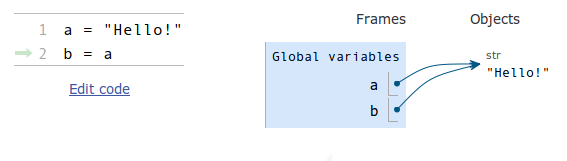
\includegraphics[width=\linewidth,keepaspectratio]{a=b.png}
% \end{center}
  
% The same object can be given many names!
% \end{frame}

%%%%%%%%%%%%%%%%%%%%%%%%%%%%%%%%%%%%%%%%%%%%%%%%%%%%%%%%%%%%%%%%%%%%%%%%%%%%%%%%%%%
\begin{frame}[fragile]  \frametitle{The \texttt{is} operator}

  Allows to test whether two names refer  to the same object:
\begin{lstlisting}
>>> a = 1
>>> b = 1
>>> a is b
True
\end{lstlisting}

\end{frame}

% %%%%%%%%%%%%%%%%%%%%%%%%%%%%%%%%%%%%%%%%%%%%%%%%%%%%%%%%%%%%%%%%%%%%%%%%%%%%%%%%%%%
% \begin{frame}[fragile]\frametitle{Sample Program}
% \begin{itemize}
% \item Upon taking this class, you are recruited in a new hot startup. 
% \item They offer you a decent starting salary (Rs. 50K), a promised 25\% bonus, and an equity package currently worth Rs. 400K, vesting over a period of 4 years.
% \end{itemize}
% \end{frame}


% % %%%%%%%%%%%%%%%%%%%%%%%%%%%%%%%%%%%%%%%%%%%%%%%%%%%%%%%%%%%%%%%%%%%%%%%%%%%%%%%%%%%
% % \begin{frame}[fragile]\frametitle{Sample Program}
% % \begin{itemize}

% % \item You want to examine the true value of this package, so you write the following program:
% % \begin{lstlisting}
% % base_salary = 50000
% % expected_bonus = 0.25
% % equity = 400000
% % years_vesting = 4
% % \end{lstlisting}
% % \item Formula
% % \begin{lstlisting}
% % yearly_value = base_salary + expected_bonus*base_salary + equity/years_vesting
% % print("The yearly value of this offer is", yearly_value)
% % \end{lstlisting}
% % \end{itemize}
% % \end{frame}

%%%%%%%%%%%%%%%%%%%%%%%%%%%%%%%%%%%%%%%%%%%%%%%%%%%%%%%%%%%%%%%%%%%%%%%%%%%%%%%%%%%
\begin{frame}[fragile]\frametitle{Exercise, I}
\begin{itemize}
\item Assume that you go to a restaurant, and you order Rs.50 worth of food. 
\item Then you need to add the Sales Tax (8.875\%) and add a tip (say, 20\%). 
\item Write down the calculation that will print the total cost of the food.
\end{itemize}
\end{frame}
%%%%%%%%%%%%%%%%%%%%%%%%%%%%%%%%%%%%%%%%%%%%%%%%%%%%%%%%%%%%%%%%%%%%%%%%%%%%%%%%%%%
\begin{frame}[fragile]\frametitle{Exercise, II}
\begin{itemize}
\item You have a stock that closed at Rs.550 on Monday, and then closed at Rs.560 on Tuesday.
\item Calculate its daily return: the daily return is defined as the difference in the closing prices, divided by the closing price the day before.
\end{itemize}
\end{frame}

%%%%%%%%%%%%%%%%%%%%%%%%%%%%%%%%%%%%%%%%%%%%%%%%%%%%%%%%%%%%%%%%%%%%%%%%%%%%%%%%%%%
\begin{frame}[fragile]\frametitle{Exercise, III}
\begin{itemize}
\item Write a Python program to solve $(x + y) * (x + y)$
\item Write a Python program to compute the future value of a specified principal amount, rate of interest, and a number of years.  Test Data : amt = 10000, int = 3.5, years = 7.
Expected Output : 12722.79
\item Write a Python program to compute the distance between the points (x1, y1) and (x2, y2).
\end{itemize}
\end{frame}

 
\section[Constructs]{Module 3: Constructs}
%%%%%%%%%%%%%%%%%%%%%%%%%%%%%%%%%%%%%%%%%%%%%%%%%%%%%%%%%%%%%%%%%%%%%%%%%%%%%%%%%%
\begin{frame}[fragile]\frametitle{}
\begin{center}
{\Large Conditionals}
\end{center}
\end{frame}

%%%%%%%%%%%%%%%%%%%%%%%%%%%%%%%%%%%%%%%%%%%%%%%%%%%%%%%%%%%%%%%%%%%%%%%%%%%%%%%%%%%
\begin{frame}[fragile]\frametitle{Conditionals}
What can we deduce from the following text:
\begin{lstlisting}
If it rains tomorrow, I will tidy up the cellar. After this I will paint the walls. If there is some time left, I will do my tax declaration. Otherwise, I will go swimming. In the evening, I will go to the cinema with my wife!
\end{lstlisting}
\end{frame}

%%%%%%%%%%%%%%%%%%%%%%%%%%%%%%%%%%%%%%%%%%%%%%%%%%%%%%%%%%%%%%%%%%%%%%%%%%%%%%%%%%%
\begin{frame}[fragile]\frametitle{Conditionals}
  \begin{columns}[c]
    \begin{column}{0.5\linewidth}
\begin{lstlisting}
If it rains tomorrow, I will do the following:
    - tidy up the cellar 
    - paint the walls
    - If there is some time left, I will 
          - do my tax declaration
Otherwise, I will do the following:
    - go swimming
go to the cinema with my wife in the evening
\end{lstlisting}
      \end{column}
    \begin{column}{0.5\linewidth}
    \begin{center}
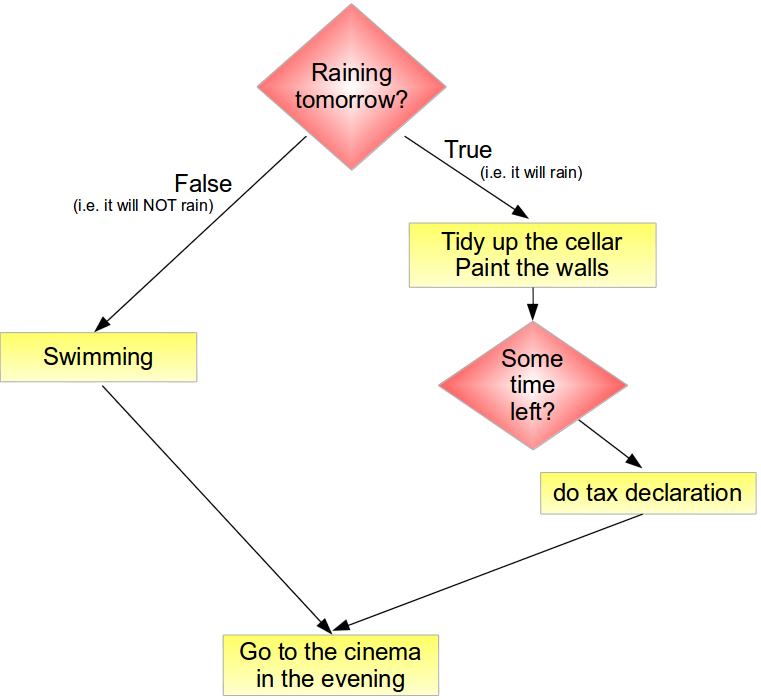
\includegraphics[width=\linewidth,keepaspectratio]{boxes8}
\end{center}
        \end{column}
  \end{columns}
\end{frame}

%%%%%%%%%%%%%%%%%%%%%%%%%%%%%%%%%%%%%%%%%%%%%%%%%%%%%%%%%%%%%%%%%%%%%%%%%%%%%%%%%%%
\begin{frame}[fragile]\frametitle{Conditionals}
  \begin{columns}[c]
    \begin{column}{0.5\linewidth}
    C:
\begin{lstlisting}
if (raining_tomorrow) {
    tidy_up_the_cellar(); 
    paint_the_walls();
    if (time_left) 
          do_taxes();
} else
    enjoy_swimming();
    go_cinema();
\end{lstlisting}
      \end{column}
    \begin{column}{0.5\linewidth}
    Python:
    \begin{lstlisting}
if raining_tomorrow:
    tidy_up_the_cellar() 
    paint_the_walls()
    if time_left: 
          do_taxes()
else:
    enjoy_swimming()
go_cinema()
\end{lstlisting}
        \end{column}
  \end{columns}
\end{frame}

%%%%%%%%%%%%%%%%%%%%%%%%%%%%%%%%%%%%%%%%%%%%%%%%%%%%%%%%%%%%%%%%%%%%%%%%%%%%%%%%%%%
\begin{frame}[fragile]\frametitle{Conditionals}
  Conditional execution uses the \texttt{if} statement:
\begin{lstlisting}
if expr:
  # indented block
elif  other-expr:
  # indented block
else:
  # executed if none of the above matched
\end{lstlisting}

The \texttt{elif} can be repeated, with different conditions, or left out entirely.
Also the \texttt{else} clause is optional.
 

Where's the `end if'?
There's no `end if': indentation delimits blocks!

\end{frame}

%%%%%%%%%%%%%%%%%%%%%%%%%%%%%%%%%%%%%%%%%%%%%%%%%%%%%%%%%%%%%%%%%%%%%%%%%%%%%%%%%%%
\begin{frame}[fragile]\frametitle{Boolean expressions}
A boolean expression is an expression that is either true or false.
\begin{lstlisting}
>>> 5 == 5
True
>>> 5 == 6
False
\end{lstlisting}
True and False are special values that belong to the class bool; they are not
strings:
\begin{lstlisting}
>>> type(True)
<class 'bool'>
>>> type(False)
<class 'bool'>
\end{lstlisting}
\end{frame}

%%%%%%%%%%%%%%%%%%%%%%%%%%%%%%%%%%%%%%%%%%%%%%%%%%%%%%%%%%%%%%%%%%%%%%%%%%%%%%%%%%%
\begin{frame}[fragile]\frametitle{Comparison operators}
== operator is one of the comparison operators; others are:
\begin{lstlisting}
x != y # x is not equal to y
x > y # x is greater than y
x < y # x is less than y
x >= y # x is greater than or equal to y
x <= y # x is less than or equal to y
x is y # x is the same as y
x is not y # x is not the same as y
\end{lstlisting}
\end{frame}

%%%%%%%%%%%%%%%%%%%%%%%%%%%%%%%%%%%%%%%%%%%%%%%%%%%%%%%%%%%%%%%%%%%%%%%%%%%%%%%%%%%
\begin{frame}[fragile]\frametitle{Logical operators}
\begin{itemize}
\item There are three logical operators: and, or, and not. 
\item \lstinline|x > 0 and x < 10| is true only if x is greater than 0 and less than 10.
\item \lstinline|n%2 == 0 or n%3 == 0| is true if either of the conditions is true, that is, if the number is divisible by 2 or 3.
%\item Finally, the not operator negates a boolean expression, so not \lstinline|(x > y)| is true if
%\lstinline|x > y| is false; that is, if x is less than or equal to y.
\end{itemize}
\end{frame}



%%%%%%%%%%%%%%%%%%%%%%%%%%%%%%%%%%%%%%%%%%%%%%%%%%%%%%%%%%%%%%%%%%%%%%%%%%%%%%%%%%%
\begin{frame}[fragile]\frametitle{Quiz: Find Largest}
Python program to find the largest number among the three input numbers
\begin{lstlisting}
num1 = 10
num2 = 14
num3 = 12

# uncomment following lines to take three numbers from user
#num1 = float(input("Enter first number: "))
#num2 = float(input("Enter second number: "))
#num3 = float(input("Enter third number: "))

\end{lstlisting}
\end{frame}


%%%%%%%%%%%%%%%%%%%%%%%%%%%%%%%%%%%%%%%%%%%%%%%%%%%%%%%%%%%%%%%%%%%%%%%%%%%%%%%%%%%
\begin{frame}[fragile]\frametitle{Solution: Find Largest}
\begin{lstlisting}

if (num1 >= num2) and (num1 >= num3):
   largest = num1
elif (num2 >= num1) and (num2 >= num3):
   largest = num2
else:
   largest = num3

print("The largest number between",num1,",",num2,"and",num3,"is",largest)
\end{lstlisting}
\end{frame}


%%%%%%%%%%%%%%%%%%%%%%%%%%%%%%%%%%%%%%%%%%%%%%%%%%%%%%%%%%%%%%%%%%%%%%%%%%%%%%%%%%%
\begin{frame}[fragile]\frametitle{Exercises}
\begin{itemize}
\item Write a Python program to get the difference between a given number and 17, if the number is greater than 17 return double the absolute difference.
\item Write a Python program to calculate the sum of three given numbers, if the values are equal then return thrice of their sum
\item Write a Python program to sum of two given integers. However, if the sum is between 15 to 20 it will return 20.
\end{itemize}
\end{frame}



%%%%%%%%%%%%%%%%%%%%%%%%%%%%%%%%%%%%%%%%%%%%%%%%%%%%%%%%%%%%%%%%%%%%%%%%%%%%%%%%%%%
\begin{frame}[fragile]\frametitle{switch/case}
  \begin{itemize}
\item There is no such statement in Python.
\item Conditional execution uses the \texttt{if} statement
\end{itemize}

\textbf{Advance:}

   It can be implemented efficiently with a dictionary of functions:
\begin{lstlisting}
result = {
	`a': lambda x: x * 5,
	'b': lambda x: x + 7,
	'c': lambda x: x - 2
}
result['b'](10)
\end{lstlisting}

\end{frame}

%%%%%%%%%%%%%%%%%%%%%%%%%%%%%%%%%%%%%%%%%%%%%%%%%%%%%%%%%%%%%%%%%%%%%%%%%%%%%%%%%%%
\begin{frame}[fragile]\frametitle{Exercises}
Rewrite your pay computation to give the employee 1.5 times the
hourly rate for hours worked above 40 hours.
\begin{lstlisting}
Enter Hours: 45
Enter Rate: 10
Pay: 475.0
\end{lstlisting}
Write a program to prompt for a score between 0.0 and 1.0. If the
score is out of range, print an error message. If the score is between 0.0 and 1.0,
print a grade using the following table:
\begin{lstlisting}
Score Grade
>= 0.9 A
>= 0.8 B
>= 0.7 C
>= 0.6 D
< 0.6 F
\end{lstlisting}

\end{frame}




%%%%%%%%%%%%%%%%%%%%%%%%%%%%%%%%%%%%%%%%%%%%%%%%%%%%%%%%%%%%%%%%%%%%%%%%%%%%%%%%%%
\begin{frame}[fragile]\frametitle{}
\begin{center}
{\Large Loops}
\end{center}
\end{frame}


%%%%%%%%%%%%%%%%%%%%%%%%%%%%%%%%%%%%%%%%%%%%%%%%%%%%%%%%%%%%%%%%%%%%%%%%%%%%%%%%%%%
\begin{frame}[fragile]\frametitle{Looping}
\begin{itemize}
\item Computers are often used to automate repetitive tasks. 
\item  Repeating identical or similar tasks without making errors is something that computers do well and people
do poorly. 
\end{itemize}
\begin{lstlisting}
n = 5
while n > 0:
	print(n)
	n = n - 1
print('Blastoff!')
\end{lstlisting}
\end{frame}



%%%%%%%%%%%%%%%%%%%%%%%%%%%%%%%%%%%%%%%%%%%%%%%%%%%%%%%%%%%%%%%%%%%%%%%%%%%%%%%%%%%
\begin{frame}[fragile]
  \frametitle{\texttt{for}-loops}
    With the  \texttt{for} statement, you can loop over the items of
    a sequence:
\begin{lstlisting}
for i in range(0, 4):
  # loop block
  print (i*i)
\end{lstlisting}

  
  To break out of a \texttt{for} loop, use the \texttt{break}
  statement.

  
  To jump to the next iteration of a \texttt{for} loop, use the
  \texttt{continue} statement.
\end{frame}

%%%%%%%%%%%%%%%%%%%%%%%%%%%%%%%%%%%%%%%%%%%%%%%%%%%%%%%%%%%%%%%%%%%%%%%%%%%%%%%%%%%
\begin{frame}[fragile]\frametitle{\texttt{for}}
  The \texttt{for} statement can be used to loop over elements in \emph{any sequence}.


\begin{lstlisting}
>>> for val in [1,2,3]:
...   print(val)
1
2
3
\end{lstlisting}
\end{frame}

%%%%%%%%%%%%%%%%%%%%%%%%%%%%%%%%%%%%%%%%%%%%%%%%%%%%%%%%%%%%%%%%%%%%%%%%%%%%%%%%%%%
\begin{frame}[fragile]\frametitle{Looping over range of numbers}
Two ways:
\begin{lstlisting}
for i in [0, 1, 2, 3, 4, 5]:
    print i**2

for i in range(6):
    print i**2
\end{lstlisting}
Better:
\begin{lstlisting}
for i in xrange(6):
    print i**2
\end{lstlisting}
xrange creates an iterator over the range producing the values one at a time. This approach is much more memory efficient than range. xrange was renamed to range in python 3

\tiny{(Ref: Transforming Code into Beautiful, Idiomatic Python -  Raymond Hettinger)}
\end{frame}

%%%%%%%%%%%%%%%%%%%%%%%%%%%%%%%%%%%%%%%%%%%%%%%%%%%%%%%%%%%%%%%%%%%%%%%%%%%%%%%%%%%
\begin{frame}[fragile]\frametitle{Looping over a collection}
``C'' way:
\begin{lstlisting}
colors = ['red', 'green', 'blue', 'yellow']

for i in range(len(colors)):
    print(colors[i])
\end{lstlisting}
Better:
\begin{lstlisting}
for color in colors:
    print(color)
\end{lstlisting}

\tiny{(Ref: Transforming Code into Beautiful, Idiomatic Python -  Raymond Hettinger)}
\end{frame}

%%%%%%%%%%%%%%%%%%%%%%%%%%%%%%%%%%%%%%%%%%%%%%%%%%%%%%%%%%%%%%%%%%%%%%%%%%%%%%%%%%%
\begin{frame}[fragile]\frametitle{\texttt{for}}
  The \texttt{for} statement can be used to loop over elements in \emph{any sequence}.

\begin{lstlisting}
>>> for val in {'UZH'}:
...   print(val)
'U'
'Z'
'H'
\end{lstlisting}

\end{frame}

%%%%%%%%%%%%%%%%%%%%%%%%%%%%%%%%%%%%%%%%%%%%%%%%%%%%%%%%%%%%%%%%%%%%%%%%%%%%%%%%%%%
\begin{frame}[fragile]\frametitle{Looping backwards}
``C'' way:
\begin{lstlisting}
colors = ['red', 'green', 'blue', 'yellow']

for i in range(len(colors)-1, -1, -1):
    print(colors[i])
\end{lstlisting}
Better:
\begin{lstlisting}
for color in reversed(colors):
    print(color)
\end{lstlisting}

\tiny{(Ref: Transforming Code into Beautiful, Idiomatic Python -  Raymond Hettinger)}
\end{frame}






%%%%%%%%%%%%%%%%%%%%%%%%%%%%%%%%%%%%%%%%%%%%%%%%%%%%%%%%%%%%%%%%%%%%%%%%%%%%%%%%%%%
\begin{frame}[fragile]\frametitle{Sorted}

  If you want to loop over a \textit{sorted} sequence you can use the
  function \texttt{sorted()} :

  \begin{lstlisting}
>>> for val in sorted([1,3,4,2]):
...  print(val)
1
2
3
4
  \end{lstlisting}

and to loop over a sequence in \textit{inverted} order you can use the
\texttt{reversed()} function:

\begin{lstlisting}
>>> for val in reversed([1,3,4,2]):
...     print(val)
2
4
3
1
\end{lstlisting}

\end{frame}

%%%%%%%%%%%%%%%%%%%%%%%%%%%%%%%%%%%%%%%%%%%%%%%%%%%%%%%%%%%%%%%%%%%%%%%%%%%%%%%%%%%
\begin{frame}[fragile]\frametitle{Looping over a collection and indices}
``C'' way:
\begin{lstlisting}
colors = ['red', 'green', 'blue', 'yellow']

for i in range(len(colors)):
    print(i, '--->', colors[i])
\end{lstlisting}
Better:
\begin{lstlisting}
for i, color in enumerate(colors):
    print(i, '--->', color)
\end{lstlisting}

It's fast and beautiful and saves you from tracking the individual indices and incrementing them.

Whenever you find yourself manipulating indices [in a collection], you're probably doing it wrong


\tiny{(Ref: Transforming Code into Beautiful, Idiomatic Python -  Raymond Hettinger)}
\end{frame}

%%%%%%%%%%%%%%%%%%%%%%%%%%%%%%%%%%%%%%%%%%%%%%%%%%%%%%%%%%%%%%%%%%%%%%%%%%%%%%%%%%%
\begin{frame}[fragile]\frametitle{Looping over two collections}
``C'' way:
\begin{lstlisting}
names = ['raymond', 'rachel', 'matthew']
colors = ['red', 'green', 'blue', 'yellow']

n = min(len(names), len(colors))
for i in range(n):
    print(names[i], '--->', colors[i])

for name, color in zip(names, colors):
    print(name, '--->', color)
\end{lstlisting}
Better:
\begin{lstlisting}
for name, color in zip(names, colors):
    print(name, '--->', color)
\end{lstlisting}

zip creates a new list in memory and takes more memory. izip is more efficient than zip. Note: in python 3 izip was renamed to zip and promoted to a builtin replacing the old zip.


\tiny{(Ref: Transforming Code into Beautiful, Idiomatic Python -  Raymond Hettinger)}
\end{frame}


%%%%%%%%%%%%%%%%%%%%%%%%%%%%%%%%%%%%%%%%%%%%%%%%%%%%%%%%%%%%%%%%%%%%%%%%%%%%%%%%%%%
\begin{frame}[fragile]\frametitle{Looping}
  Conditional looping uses the \lstinline{while} statement:
\begin{lstlisting}
while expr:
  # indented block
 else:
   # executed at natural end of the loop
\end{lstlisting}

\begin{itemize}
\item To break loop, use the \lstinline{break} statement.
\item Use \lstinline{continue} anywhere inside to jump back to the \lstinline{while}.
\item If a loop is exited via a \lstinline{break} statement, the \lstinline{else} is not executed.
\item \lstinline{else} is optional.
\end{itemize}

\end{frame}


%%%%%%%%%%%%%%%%%%%%%%%%%%%%%%%%%%%%%%%%%%%%%%%%%%%%%%%%%%%%%%%%%%%%%%%%%%%%%%%%%%%
\begin{frame}[fragile]\frametitle{Looping Exercises}
\begin{itemize}
\item Write a Python program to count the number 4 in a given list. 
\item Write a Python program to create a histogram from a given list of integers.
\end{itemize}
\end{frame}



%%%%%%%%%%%%%%%%%%%%%%%%%%%%%%%%%%%%%%%%%%%%%%%%%%%%%%%%%%%%%%%%%%%%%%%%%%%%%%%%%%%
\begin{frame}[fragile]\frametitle{Looping}
To find the largest value in a list or sequence, we construct the following loop:
\begin{lstlisting}
largest = None
print('Before:', largest)
for itervar in [3, 41, 12, 9, 74, 15]:
	if largest is None or itervar > largest :
		largest = itervar
	print('Loop:', itervar, largest)
print('Largest:', largest)
\end{lstlisting}
Finding smallest, the code is very similar with one small change:
\begin{lstlisting}
smallest = None
print('Before:', smallest)
for itervar in [3, 41, 12, 9, 74, 15]:
	if smallest is None or itervar < smallest:
		smallest = itervar
	print('Loop:', itervar, smallest)
print('Smallest:', smallest)
\end{lstlisting}
\end{frame}

%%%%%%%%%%%%%%%%%%%%%%%%%%%%%%%%%%%%%%%%%%%%%%%%%%%%%%%%%%%%%%%%%%%%%%%%%%%%%%%%%%%
\begin{frame}[fragile]\frametitle{Maximum and minimum loops}
Automatic Stop:
\begin{lstlisting}
n = 10
while n:
	print(n)
	n = n - 1
print('Done!')
\end{lstlisting}
Forced stop:
\begin{lstlisting}
while True:
	line = input('> ')
	if line == 'done':
		break
	print(line)
print('Done!')
\end{lstlisting}
\end{frame}

%%%%%%%%%%%%%%%%%%%%%%%%%%%%%%%%%%%%%%%%%%%%%%%%%%%%%%%%%%%%%%%%%%%%%%%%%%%%%%%%%%%
\begin{frame}[fragile]\frametitle{Guess the number}

Output looks like this:
\begin{lstlisting}
Hello! What is your name?
Albert
Well, Albert, I am thinking of a number between 1 and 20.
Take a guess.
10
Your guess is too high.
Take a guess.
2
Your guess is too low.
Take a guess.
4
Good job, Albert! You guessed my number in 3 guesses!
\end{lstlisting}
Write the program to do this. Use `random' module to get the secret number.
\end{frame}


%%%%%%%%%%%%%%%%%%%%%%%%%%%%%%%%%%%%%%%%%%%%%%%%%%%%%%%%%%%%%%%%%%%%%%%%%%%%%%%%%%%
\begin{frame}[fragile]\frametitle{Guess the number}
\begin{lstlisting}
import random
guessesTaken = 0
number = random.randint(1, 20)
print('Think a number between 1 and 20.')
while guessesTaken < 6:
     print('Take a guess.') 
     guess = input()
     guess = int(guess)
     guessesTaken = guessesTaken + 1
     if guess < number:
         print('Your guess is too low.') 
     if guess > number:
        print('Your guess is too high.')
     if guess == number:
         break
if guess == number:
     guessesTaken = str(guessesTaken)
     print(`You guessed in ' + guessesTaken + ' guesses!')
if guess != number:
     number = str(number)
     print('Nope. The number I was thinking of was ' + number)
\end{lstlisting}
\end{frame}

%%%%%%%%%%%%%%%%%%%%%%%%%%%%%%%%%%%%%%%%%%%%%%%%%%%%%%%%%%%%%%%%%%%%%%%%%%%%%%%%%%%
\begin{frame}[fragile]\frametitle{Quiz: Matrix Multiplication}
Given X and Y write code to do matrix multiplication
\begin{lstlisting}
X = [[12,7,3],
    [4 ,5,6],
    [7 ,8,9]]

Y = [[5,8,1,2],
    [6,7,3,0],
    [4,5,9,1]]

result = [[0,0,0,0],
         [0,0,0,0],
         [0,0,0,0]]
\end{lstlisting}

\end{frame}

%%%%%%%%%%%%%%%%%%%%%%%%%%%%%%%%%%%%%%%%%%%%%%%%%%%%%%%%%%%%%%%%%%%%%%%%%%%%%%%%%%%
\begin{frame}[fragile]\frametitle{Solution : Matrix Multiplication}

\begin{lstlisting}
for i in range(len(X)):
    for j in range(len(Y[0])):
        for k in range(len(Y)):
            result[i][j] += X[i][k] * Y[k][j]

for r in result:
    print(r)
\end{lstlisting}

\end{frame}
% %%%%%%%%%%%%%%%%%%%%%%%%%%%%%%%%%%%%%%%%%%%%%%%%%%%%%%%%%%%%%%%%%%%%%%%%%%%%%%%%%%%
% \begin{frame}[fragile]\frametitle{Unpacking}
% The  \lstinline{for}:  statement can also do unpacking. Example:
% \begin{lstlisting}
% items = ['apple', 'banana', 'cherry', 'date']
% for idx, item in enumerate(items):
	% print('{}. {}'.format(idx, item))
	
% 0.  apple
% 1.  banana
% 2.  cherry
% 3.  date
% \end{lstlisting}

% \begin{itemize}
% \item \lstinline|[f(x) for x in iterable]|
% \item \lstinline|[f(x) for x in iterable  if t(x)]|
% \end{itemize}

% \end{frame}


% %%%%%%%%%%%%%%%%%%%%%%%%%%%%%%%%%%%%%%%%%%%%%%%%%%%%%%%%%%%%%%%%%%%%%%%%%%%%%%%%%%%
% \begin{frame}[fragile]\frametitle{Generator}
% Generator expressions -- A generator expression looks similar to a list comprehension, except that it is surrounded by parentheses rather than square
% brackets. Example:
% \begin{lstlisting}
% items = ['apple', 'banana', 'cherry', 'date']
% gen1 = (item.upper() for item in items)
% for x in gen1:
	% print('x: {}'.format(x))
	
% x: APPLE
% x: BANANA
% x: CHERRY
% x: DATE
% \end{lstlisting}
% \end{frame}


\section[Seq]{Module 4: Collections}
%%%%%%%%%%%%%%%%%%%%%%%%%%%%%%%%%%%%%%%%%%%%%%%%%%%%%%%%%%%%%%%%%%%%%%%%%%%%%%%%%%
\begin{frame}[fragile]\frametitle{}
\begin{center}
{\Large Sequences}
\end{center}
\end{frame}

%%%%%%%%%%%%%%%%%%%%%%%%%%%%%%%%%%%%%%%%%%%%%%%%%%%%%%%%%%%%%%%%%%%%%%%%%%%%%%%%%%
\begin{frame}[fragile]\frametitle{}
\begin{center}
{\Large Lists}
\end{center}
\end{frame}

%%%%%%%%%%%%%%%%%%%%%%%%%%%%%%%%%%%%%%%%%%%%%%%%%%%%%%%%%%%%%%%%%%%%%%%%%%%%%%%%%%%
\begin{frame}[fragile]\frametitle{Built-in Sequences}

  \begin{itemize}
  \item {\bf list} \emph{mutable}, possibly heterogeneous
  \item{\bf tuple} \emph{immutable}, possibly heterogeneous
  \item{\bf str} \emph{immutable}, only holds characters
  \end{itemize}
\end{frame}


%%%%%%%%%%%%%%%%%%%%%%%%%%%%%%%%%%%%%%%%%%%%%%%%%%%%%%%%%%%%%%%%%%%%%%%%%%%%%%%%%%%
\begin{frame}[fragile]\frametitle{Sequences from Other Packages}
  \begin{itemize}
  \item \href{http://numpy.scipy.org}{NumPy}: {\bf array} \emph{mutable}, homogeneous (like C/Fortran arrays)
  \item Collections: OrderedDict
  \end{itemize}
\end{frame}

%%%%%%%%%%%%%%%%%%%%%%%%%%%%%%%%%%%%%%%%%%%%%%%%%%%%%%%%%%%%%%%%%%%%%%%%%%%%%%%%%%%
\begin{frame}[fragile]\frametitle{Lists}
  \begin{itemize}
  \item Ordered collections of arbitrary objects
  \item Accessed by offset
  \item Variable length, heterogeneous, arbitrarily nest-able
  \item Mutable sequence
  % \item Arrays of object references
  \end{itemize}
  \begin{lstlisting}
[10, 20, 30, 40]
['crunchy frog', 'ram bladder', 'lark vomit']
['spam', 2.0, 5, [10, 20]]
\end{lstlisting}
\end{frame}

%%%%%%%%%%%%%%%%%%%%%%%%%%%%%%%%%%%%%%%%%%%%%%%%%%%%%%%%%%%%%%%%%%%%%%%%%%%%%%%%%%%
\begin{frame}[fragile]\frametitle{List mutation}
Replace items by assigning them
  a new value:
\begin{lstlisting}
>>> L = ['U', 'Z', 'H']
>>> L[2] = 'G'
>>> print(L)
['U', 'Z', 'G']
\end{lstlisting}
Try negative indices.
\end{frame}

%%%%%%%%%%%%%%%%%%%%%%%%%%%%%%%%%%%%%%%%%%%%%%%%%%%%%%%%%%%%%%%%%%%%%%%%%%%%%%%%%%%
\begin{frame}[fragile]\frametitle{List mutation}

Replace an entire slice:
\begin{lstlisting}
>>> L[1:3] = ['a', 'b']
>>> print(L)
['U', 'a', 'b']
\end{lstlisting}
The range on the left is replaced by range on the right. If there is mismatch in the lengths? Try \ldots. 

Try negative ranges as well. If the range evaluates to null (L[-1:-2]) then right hand array is inserted at the -2 position?
\end{frame}


%%%%%%%%%%%%%%%%%%%%%%%%%%%%%%%%%%%%%%%%%%%%%%%%%%%%%%%%%%%%%%%%%%%%%%%%%%%%%%%%%%%
\begin{frame}[fragile]\frametitle{List mutation}
New slice does not need to have the same length:
\begin{lstlisting}
>>> L[2:] = range(4)
>>> print(L)
['U', 'a', 0, 1, 2, 3]
\end{lstlisting}
From 2 onwards there are only 1 (last) element, in its place put all of the right hand side, ie, array from 0 to 4.
\end{frame}

%%%%%%%%%%%%%%%%%%%%%%%%%%%%%%%%%%%%%%%%%%%%%%%%%%%%%%%%%%%%%%%%%%%%%%%%%%%%%%%%%%%
\begin{frame}[fragile]\frametitle{List mutation}
Add an element
\begin{lstlisting}
>>> L.append(4)
>>> L
['a', 0, 1, 2, 3, 4]
\end{lstlisting}
Return type of append() is None. It mutates the list itself. It does NOT return the modified list (like Strings).

So don't do:

\begin{lstlisting}
L = L.append(4)
\end{lstlisting}

\end{frame}

%%%%%%%%%%%%%%%%%%%%%%%%%%%%%%%%%%%%%%%%%%%%%%%%%%%%%%%%%%%%%%%%%%%%%%%%%%%%%%%%%%%
\begin{frame}[fragile]\frametitle{List mutation}
Remove individual items from a list either by specifying the item:
\begin{lstlisting}
>>> L.remove('U')
>>> L
['a', 0, 1, 2, 3, 4]
\end{lstlisting}
\end{frame}

%%%%%%%%%%%%%%%%%%%%%%%%%%%%%%%%%%%%%%%%%%%%%%%%%%%%%%%%%%%%%%%%%%%%%%%%%%%%%%%%%%%
\begin{frame}[fragile]\frametitle{List mutation}
or the position:

\begin{lstlisting}
>>> L.pop(1)
0
>>> L
['a', 1, 2, 3, 4]
\end{lstlisting}
\end{frame}

%%%%%%%%%%%%%%%%%%%%%%%%%%%%%%%%%%%%%%%%%%%%%%%%%%%%%%%%%%%%%%%%%%%%%%%%%%%%%%%%%%%
\begin{frame}[fragile]\frametitle{List mutation}

Note: \texttt{remove()} method only removes \textit{the first occurrence}:

\begin{lstlisting}
>>> L = ['a', 'b', 'a']
>>> L.remove('a')
>>> L
['b', 'a']
\end{lstlisting}

\end{frame}

%%%%%%%%%%%%%%%%%%%%%%%%%%%%%%%%%%%%%%%%%%%%%%%%%%%%%%%%%%%%%%%%%%%%%%%%%%%%%%%%%%%
\begin{frame}[fragile]\frametitle{List mutation}

``del'' operator can be used two ways:

Remoes definition of 2nd position, thus the list shrinks.

\begin{lstlisting}
>>> L = ['a', 'b', 'a']
>>> del L[1]
>>> L
['a', 'a']
\end{lstlisting}

Remove the definition of whole list:
\begin{lstlisting}
>>> del L
>>> L
"Not defined error"
\end{lstlisting}

\end{frame}

%%%%%%%%%%%%%%%%%%%%%%%%%%%%%%%%%%%%%%%%%%%%%%%%%%%%%%%%%%%%%%%%%%%%%%%%%%%%%%%%%%%
\begin{frame}[fragile]\frametitle{List Sorting}

Dont use old L.sort() method but newer sorted method.

Here sorted returns the copy of the sorted list keeping original intact.

\begin{lstlisting}
>>> L = [5,3,4,7]
>>> M = sorted(L)
>>> L
[5,3,4,7]
>>> M
[3,4,5,7]
\end{lstlisting}

\end{frame}

%%%%%%%%%%%%%%%%%%%%%%%%%%%%%%%%%%%%%%%%%%%%%%%%%%%%%%%%%%%%%%%%%%%%%%%%%%%%%%%%%%%
\begin{frame}[fragile]\frametitle{List Sorting}

Applies to strings also. The sorted() function can be customized through optional arguments. The sorted() optional argument reverse=True, e.g. sorted(list, reverse=True), makes it sort backwards.

\begin{lstlisting}
strs = ['aa', 'BB', 'zz', 'CC']
  print sorted(strs)  ## ['BB', 'CC', 'aa', 'zz'] (case sensitive)
  print sorted(strs, reverse=True)   ## ['zz', 'aa', 'CC', 'BB']
\end{lstlisting}

\end{frame}

%%%%%%%%%%%%%%%%%%%%%%%%%%%%%%%%%%%%%%%%%%%%%%%%%%%%%%%%%%%%%%%%%%%%%%%%%%%%%%%%%%%
\begin{frame}[fragile]\frametitle{List Custom Sorting With key=}

\begin{itemize}
\item For more complex custom sorting, sorted() takes an optional "key=" specifying a "key" function that transforms each element before comparison. The key function takes in 1 value and returns 1 value, and the returned "proxy" value is used for the comparisons within the sort.

\item For example with a list of strings, specifying key=len (the built in len() function) sorts the strings by length, from shortest to longest. The sort calls len() for each string to get the list of proxy length values, and then sorts with those proxy values.
\end{itemize}

\begin{lstlisting}
  strs = ['ccc', 'aaaa', 'd', 'bb']
  print sorted(strs, key=len)  ## ['d', 'bb', 'ccc', 'aaaa']
\end{lstlisting}

\begin{center}
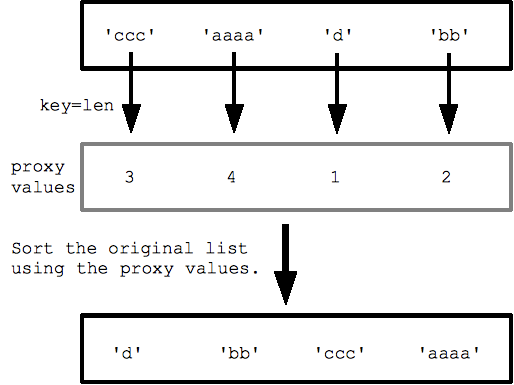
\includegraphics[width=0.6\linewidth,keepaspectratio]{custsort}
\end{center}

\tiny{(Ref: Google Python class)}
\end{frame}


%%%%%%%%%%%%%%%%%%%%%%%%%%%%%%%%%%%%%%%%%%%%%%%%%%%%%%%%%%%%%%%%%%%%%%%%%%%%%%%%%%%
\begin{frame}[fragile]\frametitle{Lists operators}
  You can concatenate two lists using the \texttt{+} operator:
  \begin{lstlisting}
>>> [1, 2] + [3, 4]
[1, 2, 3, 4]
  \end{lstlisting}
\end{frame}


%%%%%%%%%%%%%%%%%%%%%%%%%%%%%%%%%%%%%%%%%%%%%%%%%%%%%%%%%%%%%%%%%%%%%%%%%%%%%%%%%%%
\begin{frame}[fragile]\frametitle{Lists operators}
  You can mutate a list in place with the \texttt{+=} operator:
  \begin{lstlisting}
>>> L = [1, 2]
>>> L += [3, 4]
>>> print(L)
[1, 2, 3, 4]
  \end{lstlisting}
\end{frame}

%%%%%%%%%%%%%%%%%%%%%%%%%%%%%%%%%%%%%%%%%%%%%%%%%%%%%%%%%%%%%%%%%%%%%%%%%%%%%%%%%%%
\begin{frame}[fragile]\frametitle{Lists operators}
The \texttt{*} operator also works on lists:
  \begin{lstlisting}
>>> L = [1, 2]
>>> print(L*3)
[1, 2, 1, 2, 1, 2 ]
  \end{lstlisting}
\end{frame}

%%%%%%%%%%%%%%%%%%%%%%%%%%%%%%%%%%%%%%%%%%%%%%%%%%%%%%%%%%%%%%%%%%%%%%%%%%%%%%%%%%%
\begin{frame}[fragile]\frametitle{Traversing a list}
  Most common, for loop:
  \begin{lstlisting}
for cheese in cheeses:
    print(cheese)

for i in range(len(numbers)):
    numbers[i] = numbers[i] * 2
    
for x in empty:
	print('This never happens.')    
  \end{lstlisting}
\end{frame}



%%%%%%%%%%%%%%%%%%%%%%%%%%%%%%%%%%%%%%%%%%%%%%%%%%%%%%%%%%%%%%%%%%%%%%%%%%%%%%%%%%%
\begin{frame}[fragile]\frametitle{Exercise}
Take two lists, say for example these two:

  a = [1, 1, 2, 3, 5, 8, 13, 21, 34, 55, 89]
  b = [1, 2, 3, 4, 5, 6, 7, 8, 9, 10, 11, 12, 13]
  
and write a program that returns a list that contains only the elements that are common between the lists (without duplicates). Make sure your program works on two lists of different sizes.
\end{frame}

%%%%%%%%%%%%%%%%%%%%%%%%%%%%%%%%%%%%%%%%%%%%%%%%%%%%%%%%%%%%%%%%%%%%%%%%%%%%%%%%%%%
\begin{frame}[fragile]\frametitle{Lists and functions}
  \begin{lstlisting}
>>> nums = [3, 41, 12, 9, 74, 15]
>>> print(len(nums))
6
>>> print(max(nums))
74
>>> print(min(nums))
3
>>> print(sum(nums))
154
>>> print(sum(nums)/len(nums))
25
  \end{lstlisting}
\end{frame}

%%%%%%%%%%%%%%%%%%%%%%%%%%%%%%%%%%%%%%%%%%%%%%%%%%%%%%%%%%%%%%%%%%%%%%%%%%%%%%%%%%%
\begin{frame}[fragile]\frametitle{Average}
  \begin{lstlisting}
total = 0
count = 0

while (True):
	inp = input('Enter a number: ')
	if inp == 'done': break
	value = float(inp)
	total = total + value
	count = count + 1
	
average = total / count
print('Average:', average)
  \end{lstlisting}
\end{frame}


%%%%%%%%%%%%%%%%%%%%%%%%%%%%%%%%%%%%%%%%%%%%%%%%%%%%%%%%%%%%%%%%%%%%%%%%%%%%%%%%%%%
\begin{frame}[fragile]\frametitle{The `{\ttfamily\bfseries in}' operator}

  To test for presence of an item in a collection:

  \begin{itemize}
  \item {\bf x in S}:   Evaluates to \texttt{True} if \texttt{x} is equal to a \emph{value}
    contained in the \texttt{S} sequence (list, tuple, set).
\item {\bf x in T}: Evaluates to \texttt{True} if \texttt{x} is a substring of
    string \texttt{T}.
  \end{itemize}

\end{frame}


%%%%%%%%%%%%%%%%%%%%%%%%%%%%%%%%%%%%%%%%%%%%%%%%%%%%%%%%%%%%%%%%%%%%%%%%%%%%%%%%%%%
\begin{frame}[fragile]\frametitle{The \texttt{in} operator and the \texttt{if} conditional}

  Testing for the existence of an element in a container is a very
  common pattern:
  \texttt{in} operator:

\begin{lstlisting}
>>> L = [1, 2, 3, 4]
>>> if 1 in L:
...   print("Found!")
...
Found!
\end{lstlisting}
\end{frame}


%%%%%%%%%%%%%%%%%%%%%%%%%%%%%%%%%%%%%%%%%%%%%%%%%%%%%%%%%%%%%%%%%%%%%%%%%%%%%%%%%%%
\begin{frame}[fragile]\frametitle{The \texttt{in} operator and the \texttt{if} conditional}

Equivalent to the following, more verbose, less \textit{pythonic}:
 \begin{lstlisting}
 >>> L = [1, 2, 3, 4]
 >>> for item in L:
 ...     if item == 1:
 ...         print("Found!")
 ...         break
 \end{lstlisting}
\end{frame}


%%%%%%%%%%%%%%%%%%%%%%%%%%%%%%%%%%%%%%%%%%%%%%%%%%%%%%%%%%%%%%%%%%%%%%%%%%%%%%%%%%%
\begin{frame}[fragile]\frametitle{Zip and Argument Unpacking}
  \begin{itemize}
  \item zip transforms multiple lists into a single list of tuples
  \begin{lstlisting}
list1 = ['a', 'b', 'c']
list2 = [1, 2, 3]
zip(list1, list2) # is [('a', 1), ('b', 2), ('c', 3)]
  \end{lstlisting}
\item 	If the	lists are different lengths, zip stops as soon as the first list ends.
\item You can also unzip
  \begin{lstlisting}
pairs = [('a', 1), ('b', 2), ('c', 3)]
letters, numbers = zip(*pairs)
  \end{lstlisting}
\item The asterisk performs argument unpacking. Whats the ``type'' of ``letters'' and ``numbers''?
  \end{itemize}
\end{frame}

%%%%%%%%%%%%%%%%%%%%%%%%%%%%%%%%%%%%%%%%%%%%%%%%%%%%%%%%%%%%%%%%%%%%%%%%%%%%%%%%%%%
\begin{frame}[fragile]\frametitle{Lists and strings}
  \begin{itemize}
  \item String: sequence of characters
  \item List: sequence of values
  \item A list of characters is not the same as a string. 
  \item To convert from a string to a list of characters:
  \end{itemize}
    \begin{lstlisting}
>>> s = 'spam'
>>> t = list(s) #The list function breaks a string into individual letters.
>>> print(t)
['s', 'p', 'a', 'm']
  \end{lstlisting}
\end{frame}

%%%%%%%%%%%%%%%%%%%%%%%%%%%%%%%%%%%%%%%%%%%%%%%%%%%%%%%%%%%%%%%%%%%%%%%%%%%%%%%%%%%
\begin{frame}[fragile]\frametitle{Lists and strings}
  `Split' to break a string into list of words:
     \begin{lstlisting}
>>> s = 'pining for the fjords'
>>> t = s.split()
>>> print(t)
['pining', 'for', 'the', 'fjords']
>>> print(t[2])
  \end{lstlisting}
\end{frame}



%%%%%%%%%%%%%%%%%%%%%%%%%%%%%%%%%%%%%%%%%%%%%%%%%%%%%%%%%%%%%%%%%%%%%%%%%%%%%%%%%%%
\begin{frame}[fragile]\frametitle{Lists Exercise}
  \begin{itemize}
  \item Download www.py4e.com/code3/romeo.txt
  \item Open the file and read it line by line. 
  \item Split each line into a list of words using the split function.
  \item For each word, check to see if the word is already in a list. 
  \item If the word is not in the list, add it to the list.
  \item Sort and print the resulting words in alphabetical order.
  \end{itemize}
\end{frame}

%%%%%%%%%%%%%%%%%%%%%%%%%%%%%%%%%%%%%%%%%%%%%%%%%%%%%%%%%%%%%%%%%%%%%%%%%%%%%%%%%%%
\begin{frame}[fragile]\frametitle{Lists Exercise}
  \begin{lstlisting}
Enter file: romeo.txt
['Arise', 'But', 'It', 'Juliet', 'Who', 'already',
'and', 'breaks', 'east', 'envious', 'fair', 'grief',
'is', 'kill', 'light', 'moon', 'pale', 'sick', 'soft',
'sun', 'the', 'through', 'what', 'window',
'with', 'yonder']
  \end{lstlisting}
\end{frame}


%%%%%%%%%%%%%%%%%%%%%%%%%%%%%%%%%%%%%%%%%%%%%%%%%%%%%%%%%%%%%%%%%%%%%%%%%%%%%%%%%%%
\begin{frame}[fragile]\frametitle{Lists operations (recap)}
  \begin{itemize}
  \item empty list \lstinline{L = []}
  \item four items \lstinline{L2 = [0, 1, 2, 3]}
  \item nested \lstinline{L3 = ['abc', ['def', 'ghi']]}
  \item index \lstinline{L2[i], L3[i][j]}
  \item slice, length \lstinline{L2[i:j], len(L2)}
  \item concatenate, repeat \lstinline{L1 + L2, L2 * 3}
  \item iteration, membership \lstinline{for x in L2, 3 in L2}
  \item methods \lstinline{L2.append(4), L2.sort(), L2.index(1), L2.reverse()}
  \item shrinking \lstinline{del L2[k], L2[i:j] = []}
  \item assignment \lstinline{L2[i] = 1, L2[i:j] = [4,5,6]}
  \item create list \lstinline{range(4) # useful to loop}
  \end{itemize}
\end{frame}

%%%%%%%%%%%%%%%%%%%%%%%%%%%%%%%%%%%%%%%%%%%%%%%%%%%%%%%%%%%%%%%%%%%%%%%%%%%%%%%%%%
\begin{frame}[fragile]\frametitle{}
\begin{center}
{\Large Sequences: List Comprehensions}
\end{center}
\end{frame}

%%%%%%%%%%%%%%%%%%%%%%%%%%%%%%%%%%%%%%%%%%%%%%%%%%%%%%%%%%%%%%%%%%%%%%%%%%%%%%%%%%%
\begin{frame}[fragile]\frametitle{List Comprehensions}
  \begin{itemize}
  \item Compact syntax for \emph{filtering} elements  of a list and/or \emph{applying} a function to them.
\item To build a list.
\end{itemize}
Say, you wish to build a list of squares fro 0 to 5.
  \begin{lstlisting}
data = []
for num in range(6):
    data.append(num*num)
  \end{lstlisting}
  
 Can be written using \textit{list comprehension}:
  \begin{lstlisting}
data = [num*num for num in range(6) ]
  \end{lstlisting}

\end{frame}

%%%%%%%%%%%%%%%%%%%%%%%%%%%%%%%%%%%%%%%%%%%%%%%%%%%%%%%%%%%%%%%%%%%%%%%%%%%%%%%%%%%
\begin{frame}[fragile]\frametitle{List Comprehensions}
Say, you wish to build a list of squares fro 0 to 5, only for even numbers.
  \begin{lstlisting}
data = []
for num in range(6):
    if num%2==0:
        data.append(num*num)
  \end{lstlisting}
  
 Can be written using \textit{list comprehension}:
  \begin{lstlisting}
data = [num*num for num in range(6) if num%2==0 ]
  \end{lstlisting}

\end{frame}

%%%%%%%%%%%%%%%%%%%%%%%%%%%%%%%%%%%%%%%%%%%%%%%%%%%%%%%%%%%%%%%%%%%%%%%%%%%%%%%%%%%
\begin{frame}[fragile]\frametitle{Example: List Comprehensions}
 
Download  https://raw.github.com/gc3-uzh-ch/python-course/master/values.dat.

Build its list.
  \begin{lstlisting}
data = []
for num in open('values.dat').readlines():
    data.append(int(num))
  \end{lstlisting}
  
 Can be written using \textit{list comprehension}:
  \begin{lstlisting}
data = [ int(line) for line in open('values.dat').readlines() ]
  \end{lstlisting}

\end{frame}

%%%%%%%%%%%%%%%%%%%%%%%%%%%%%%%%%%%%%%%%%%%%%%%%%%%%%%%%%%%%%%%%%%%%%%%%%%%%%%%%%%%
\begin{frame}[fragile]\frametitle{List comprehensions}
  \def\e{\ttfamily\itshape}

  The general syntax of a list comprehension is:
  \begin{lstlisting}
    [expr for var in iterable if condition]
  \end{lstlisting}
  where:
  \begin{itemize}
  \item{\bf expr} is any Python expression;
  \item{\bf iterable} is a (generalized) sequence;
  \item {\bf condition} is a boolean expression, depending on
    {\e var};
  \item {\bf var} is a variable that will be bound in turn to each item
    in {\e iterable} which satisfies {\e condition}.
  \end{itemize}

   \textit{Create a new list, and for each \textbf{var} in the
    sequence \textbf{iterable}, if \textbf{condition} is true then add
    \textbf{expr} to the list.}
\end{frame}

%%%%%%%%%%%%%%%%%%%%%%%%%%%%%%%%%%%%%%%%%%%%%%%%%%%%%%%%%%%%%%%%%%%%%%%%%%%%%%%%%%%
\begin{frame}[fragile]\frametitle{List comprehensions}
Need not use all the values
  \begin{lstlisting}
zeros = [0 for _ in even_numbers] # just to have same size
  \end{lstlisting}
Mutliple for loops:
  \begin{lstlisting}
pairs = [(x,y)
		for x in range(10)
			for y in range(10)] # 100 pairs of [(0,0), (0,1)...]
  \end{lstlisting}
\end{frame}

%%%%%%%%%%%%%%%%%%%%%%%%%%%%%%%%%%%%%%%%%%%%%%%%%%%%%%%%%%%%%%%%%%%%%%%%%%%%%%%%%%%
\begin{frame}[fragile]\frametitle{Exercise}
  \begin{itemize}
  \item Write a program which will find all such numbers which are divisible by 7 but are not a multiple of 5,
between 2000 and 3200 (both included).
  \item The numbers obtained should be printed in a comma-separated sequence on a single line.
  \item Use ``join'' to make the single string. May need to cast integers by str() to be join-able.
  \end{itemize}  
\end{frame}

%%%%%%%%%%%%%%%%%%%%%%%%%%%%%%%%%%%%%%%%%%%%%%%%%%%%%%%%%%%%%%%%%%%%%%%%%%%%%%%%%%%
\begin{frame}[fragile]\frametitle{Exercise}
  \begin{itemize}
  \item Write a program that calculates and prints the value according to the given formula:
  \item Q = Square root of [(2 * C * D)/H]
  \item The fixed values of C and H: C is 50. H is 30.
  \item D is the variable whose values should be input to your program in a comma-separated sequence.
  \item Example: Let us assume the following comma separated input sequence is given to the program: 100,150,180
  \item The output of the program should be: 18,22,24
  \item Hints: If the output received is in decimal form, it should be rounded off to its nearest value (for example, if the output received is 26.0, it should be printed as 26)
%In case of input data being supplied to the question, it should be assumed to be a console input. 
  \end{itemize}  
\end{frame}

%%%%%%%%%%%%%%%%%%%%%%%%%%%%%%%%%%%%%%%%%%%%%%%%%%%%%%%%%%%%%%%%%%%%%%%%%%%%%%%%%%%
\begin{frame}[fragile]\frametitle{Solution}
  \begin{lstlisting}
import math
c=50
h=30
value = []
items=[x for x in input("Enter : ").split(',')]
for d in items:
    value.append(str(int(round(math.sqrt(2*c*float(d)/h)))))

print(','.join(value))
  \end{lstlisting}
\end{frame}



%%%%%%%%%%%%%%%%%%%%%%%%%%%%%%%%%%%%%%%%%%%%%%%%%%%%%%%%%%%%%%%%%%%%%%%%%%%%%%%%%%%
\begin{frame}[fragile]\frametitle{Exercise}
  \begin{itemize}
  \item Write a program that accepts a comma separated sequence of words as input and prints the words in a comma-separated sequence after sorting them alphabetically.
  \item Suppose the following input is supplied to the program:without,hello,bag,world
  \item Then, the output should be: bag,hello,without,world
%  \item Hints: In case of input data being supplied to the question, it should be assumed to be a console input.
  \end{itemize}  
\end{frame}

%%%%%%%%%%%%%%%%%%%%%%%%%%%%%%%%%%%%%%%%%%%%%%%%%%%%%%%%%%%%%%%%%%%%%%%%%%%%%%%%%%%
\begin{frame}[fragile]\frametitle{Solution}
  \begin{lstlisting}
items=[x for x in input("Enter : ").split(',')]
items.sort()
print(','.join(items))
  \end{lstlisting}
\end{frame}

%%%%%%%%%%%%%%%%%%%%%%%%%%%%%%%%%%%%%%%%%%%%%%%%%%%%%%%%%%%%%%%%%%%%%%%%%%%%%%%%%%%
\begin{frame}[fragile]\frametitle{Exercise}
  \begin{itemize}
  \item Write a program that accepts a sequence of whitespace separated words as input and prints the words after removing all duplicate words and sorting them alphanumerically.
  \item Suppose the following input is supplied to the program: hello world and practice makes perfect and hello world again
  \item Then, the output should be: again and hello makes perfect practice world
%  \item Hints: In case of input data being supplied to the question, it should be assumed to be a console input.
  \item We use set container to remove duplicated data automatically and then use sorted() to sort the data.
  \end{itemize}  
\end{frame}

%%%%%%%%%%%%%%%%%%%%%%%%%%%%%%%%%%%%%%%%%%%%%%%%%%%%%%%%%%%%%%%%%%%%%%%%%%%%%%%%%%%
\begin{frame}[fragile]\frametitle{Solution}
  \begin{lstlisting}
s = input("Enter : ")
words = [word for word in s.split(" ")]
print(" ".join(sorted(list(set(words)))))
  \end{lstlisting}
\end{frame}



%%%%%%%%%%%%%%%%%%%%%%%%%%%%%%%%%%%%%%%%%%%%%%%%%%%%%%%%%%%%%%%%%%%%%%%%%%%%%%%%%%%
\begin{frame}[fragile]\frametitle{Exercise}
  \begin{itemize}
  \item Write a program which takes 2 digits, X,Y as input and generates a 2-dimensional array. The element value in the i-th row and j-th column of the array should be i*j.
  \item Note:$ i=0,1 \ldots, X-1; j=0,1, \ldots Y-1.$
  \item Example: Suppose the following inputs are given to the program: 3,5
  \item Then, the output of the program should be: [[0, 0, 0, 0, 0], [0, 1, 2, 3, 4], [0, 2, 4, 6, 8]] 
  \item Hints: Note: In case of input data being supplied to the question, it should be assumed to be a console input in a comma-separated form.

  \end{itemize}  
\end{frame}

%%%%%%%%%%%%%%%%%%%%%%%%%%%%%%%%%%%%%%%%%%%%%%%%%%%%%%%%%%%%%%%%%%%%%%%%%%%%%%%%%%%
\begin{frame}[fragile]\frametitle{Solution}
  \begin{lstlisting}
input_str = input("Enter : ")
dimensions=[int(x) for x in input_str.split(',')]
rowNum=dimensions[0]
colNum=dimensions[1]
multilist = [[0 for col in range(colNum)] for row in range(rowNum)]

for row in range(rowNum):
    for col in range(colNum):
        multilist[row][col]= row*col

print(multilist)
  \end{lstlisting}
\end{frame}
%
%
%
%%%%%%%%%%%%%%%%%%%%%%%%%%%%%%%%%%%%%%%%%%%%%%%%%%%%%%%%%%%%%%%%%%%%%%%%%%%%%%%%%%%%
%\begin{frame}[fragile]\frametitle{Generators}
%  \begin{itemize}
%  \item List can grow big, very big, which can be a huge source of inefficiency, especially if you need only few values
%   \item Generator iterate over and produce as and when needed
%   \item Create using fucntion and keyword {\em yield}
%  \begin{lstlisting}
%def lazy_range(n):
%"""a lazy version of range"""
%i = 0
%while i < n:
%    yield i
%    i += 1
%  \end{lstlisting}
%\item Following loop will consume yielded voalues, one at a time until none are left:
%  \begin{lstlisting}
%for i in lazy_range(10):
%	do_something_with(i)
%  \end{lstlisting}
%\item Pythin has ready fiunction like that called {\em xrange()}
%  \end{itemize}
%\end{frame}
%
%%%%%%%%%%%%%%%%%%%%%%%%%%%%%%%%%%%%%%%%%%%%%%%%%%%%%%%%%%%%%%%%%%%%%%%%%%%%%%%%%%%%
%\begin{frame}[fragile]\frametitle{Randomness}
%  \begin{itemize}
%  \item Many times you need to use random numbers
%  \begin{lstlisting}
%import	random
%four_uniform_randoms = [random.random() for _ in range(4)]
%# [0.8444218515250481,	 # random.random() produces numbers
%# 0.7579544029403025,	# uniformly between 0 and 1
%# 0.420571580830845, #	it's the random function we'll use
%# 0.25891675029296335]	 # most often
%  \end{lstlisting}
%\item 	Actually produces pseudorandom	(that is, deterministic) numbers based on an internal state that you can set with random.seed	
%  \begin{lstlisting}
%random.seed(10) # set the seed to 10
%print random.random() # 0.57140259469 
%random.seed(10) # reset the seed to 10
%print random.random() # 0.57140259469 again
%  \end{lstlisting}
%  \end{itemize}
%\end{frame}
%
%
%%%%%%%%%%%%%%%%%%%%%%%%%%%%%%%%%%%%%%%%%%%%%%%%%%%%%%%%%%%%%%%%%%%%%%%%%%%%%%%%%%%%
%\begin{frame}[fragile]\frametitle{Exercises}
%\begin{itemize}
%\item
%    Write a function called \texttt{load\_data2(filename, bound)}
%    \item Use List  Comprehensions, 
%    \item Read  https://raw.github.com/gc3-uzh-ch/python-course/master/values.dat
%    \item Has one  integer number per line, and return a list of the integer values
%
%    \begin{lstlisting}
%>>> load_data2('values.dat', 300000)
%[299850, 299740, 299900, 299930]
%    \end{lstlisting}
%
% \end{itemize}
%\end{frame}

%
%%%%%%%%%%%%%%%%%%%%%%%%%%%%%%%%%%%%%%%%%%%%%%%%%%%%%%%%%%%%%%%%%%%%%%%%%%%%%%%%%%%%
%\begin{frame}[fragile]\frametitle{Exercises}
%\begin{itemize}
%\item Write a function \texttt{odd} that takes a list of integers and returns a list of all the odd ones.
%\item Write a function \texttt{concat} that takes a list of lists and
%    returns the concatenation of those lists. For instance:
%    \begin{lstlisting}
%>>> concat([ [1,2,3], [4,5,6], [7,8,9] ])
%[1, 2, 3, 4, 5, 6, 7, 8, 9]
%    \end{lstlisting}
%\end{itemize}
%
%
%\end{frame}


%%%%%%%%%%%%%%%%%%%%%%%%%%%%%%%%%%%%%%%%%%%%%%%%%%%%%%%%%%%%%%%%%%%%%%%%%%%%%%%%%%
\begin{frame}[fragile]\frametitle{}
\vspace{1in}
\begin{center}
{\Large Sequences: Tuples}
\end{center}
\end{frame}



%%%%%%%%%%%%%%%%%%%%%%%%%%%%%%%%%%%%%%%%%%%%%%%%%%%%%%%%%%%%%%%%%%%%%%%%%%%%%%%%%%%
\begin{frame}[fragile]\frametitle{Tuples}
  \begin{itemize}
  \item They are like lists but immutable. Why Lists and Tuples?
  \item When you want to make sure the content won't change.
  \end{itemize}
  \begin{lstlisting}
>>> T = (1, 2, 3)
>>> T[0]
1
>>> T[0:1]
(1,)
  \end{lstlisting}

\end{frame}



%%%%%%%%%%%%%%%%%%%%%%%%%%%%%%%%%%%%%%%%%%%%%%%%%%%%%%%%%%%%%%%%%%%%%%%%%%%%%%%%%%%
\begin{frame}[fragile]\frametitle{Tuples}
But they are \textit{immutable}

\begin{lstlisting}[basicstyle=\footnotesize\ttfamily]
>>> T[0] = 'a'
Traceback (most recent call last):
  File "<stdin>", line 1, in <module>
TypeError: 'tuple' object does not support item assignment
\end{lstlisting}
\end{frame}
%
%
%%%%%%%%%%%%%%%%%%%%%%%%%%%%%%%%%%%%%%%%%%%%%%%%%%%%%%%%%%%%%%%%%%%%%%%%%%%%%%%%%%%%
%\begin{frame}[fragile]\frametitle{Comparing tuples}
%The comparison operators work with tuples.
%\begin{lstlisting}[basicstyle=\footnotesize\ttfamily]
%>>> (0, 1, 2) < (0, 3, 4)
%True
%>>> (0, 1, 2000000) < (0, 3, 4)
%True
%    \end{lstlisting}
%\end{frame}
%
%
%
%%%%%%%%%%%%%%%%%%%%%%%%%%%%%%%%%%%%%%%%%%%%%%%%%%%%%%%%%%%%%%%%%%%%%%%%%%%%%%%%%%%%
%\begin{frame}[fragile]\frametitle{Comparing tuples}
%The sort function works the same way.
%    \begin{lstlisting}[basicstyle=\footnotesize\ttfamily]
%txt = 'but soft what light in yonder window'
%
%words = txt.split()
%
%t = list()
%
%for word in words:
%	t.append((len(word), word))
%	
%t.sort(reverse=True)
%
%res = list()
%for length, word in t:
%	res.append(word)
%	
%print(res)
%    \end{lstlisting}
%
%\end{frame}
%

%%%%%%%%%%%%%%%%%%%%%%%%%%%%%%%%%%%%%%%%%%%%%%%%%%%%%%%%%%%%%%%%%%%%%%%%%%%%%%%%%%%
\begin{frame}[fragile]
\frametitle{Multiple assignment}
You can assigning multiple variables at the same time
\begin{lstlisting}
>>> a, b, c = (1, 2, 3)
>>> print(a)
1
>>> print(b)
2
\end{lstlisting}
\end{frame}



%%%%%%%%%%%%%%%%%%%%%%%%%%%%%%%%%%%%%%%%%%%%%%%%%%%%%%%%%%%%%%%%%%%%%%%%%%%%%%%%%%%
\begin{frame}[fragile]
\frametitle{Multiple assignment}
It works with any sequence:

\begin{lstlisting}
>>> a, b, c = 'UZH'
>>> print(a)
U
\end{lstlisting}



  Can you think of a way to swap the values of two variables using this?


\begin{lstlisting}
>>> a, b = b, a
\end{lstlisting}
\end{frame}


%%%%%%%%%%%%%%%%%%%%%%%%%%%%%%%%%%%%%%%%%%%%%%%%%%%%%%%%%%%%%%%%%%%%%%%%%%%%%%%%%%%
\begin{frame}[fragile]\frametitle{Multiple assignment}
In \texttt{for}:
\begin{lstlisting}
>>> L = [(1,'a'), (2,'b'), (3, 'c')]
>>> for x, y in L:
...     print ("first is " + str(x)
...            + ' and second is ' + y)
\end{lstlisting}

  
Useful with functions that return a tuple.

``returning a comma separated elements creates a tuple. Multiple values can only be returned inside containers. It looks a bit peculiar, but it’s actually the comma that forms a tuple, not the parentheses''

\tiny{(Ref: How does Python return multiple values from a function? - Stack Overflow)}

\end{frame}

%%%%%%%%%%%%%%%%%%%%%%%%%%%%%%%%%%%%%%%%%%%%%%%%%%%%%%%%%%%%%%%%%%%%%%%%%%%%%%%%%%%
\begin{frame}[fragile]\frametitle{Clarify multiple return values with named tuples}
Is this good or bad? You don't know because it's not clear.
\begin{lstlisting}
# Old testmod return value
doctest.testmod()
# (0, 4)
\end{lstlisting}
Better:
\begin{lstlisting}
# New testmod return value, a namedTuple
doctest.testmod()
# TestResults(failed=0, attempted=4)
\end{lstlisting}

A namedTuple is a subclass of tuple so they still work like a regular tuple, but are more friendly. To make a namedTuple:
\begin{lstlisting}
TestResults = namedTuple('TestResults', ['failed', 'attempted'])
\end{lstlisting}

\tiny{(Ref: Transforming Code into Beautiful, Idiomatic Python -  Raymond Hettinger)}

\end{frame}

%%%%%%%%%%%%%%%%%%%%%%%%%%%%%%%%%%%%%%%%%%%%%%%%%%%%%%%%%%%%%%%%%%%%%%%%%%%%%%%%%%%
\begin{frame}[fragile]\frametitle{Unpacking sequences}
\begin{lstlisting}
p = 'Yogesh', 'Kulkarni', 0x30, 'python@example.com'

# A common approach / habit from other languages
fname = p[0]
lname = p[1]
age = p[2]
email = p[3]
\end{lstlisting}
Better:
\begin{lstlisting}
fname, lname, age, email = p
\end{lstlisting}

This approach uses tuple unpacking and is faster and more readable.

\tiny{(Ref: Transforming Code into Beautiful, Idiomatic Python -  Raymond Hettinger)}

\end{frame}

%%%%%%%%%%%%%%%%%%%%%%%%%%%%%%%%%%%%%%%%%%%%%%%%%%%%%%%%%%%%%%%%%%%%%%%%%%%%%%%%%%%
\begin{frame}[fragile]\frametitle{Exercise}
\begin{itemize}
\item Write a program which accepts a sequence of comma-separated numbers from console and generate a list and a tuple which contains every number.
\item Suppose the following input is supplied to the program: 34,67,55,33,12,98
\item Then, the output should be: ['34', '67', '55', '33', '12', '98'] ('34', '67', '55', '33', '12', '98')
%\item Hints: In case of input data being supplied to the question, it should be assumed to be a console input.
%tuple() method can convert list to tuple
\end{itemize}
\end{frame}

%%%%%%%%%%%%%%%%%%%%%%%%%%%%%%%%%%%%%%%%%%%%%%%%%%%%%%%%%%%%%%%%%%%%%%%%%%%%%%%%%%%
\begin{frame}[fragile]\frametitle{Solution}
\begin{lstlisting}
values=input("Enter : ")
l=values.split(",")
t=tuple(l)
print(l)
print(t)
\end{lstlisting}
\end{frame}

%%%%%%%%%%%%%%%%%%%%%%%%%%%%%%%%%%%%%%%%%%%%%%%%%%%%%%%%%%%%%%%%%%%%%%%%%%%%%%%%%%%%
%\begin{frame}[fragile]\frametitle{Exercises}
%
%  \begin{itemize}
%    \item
%    Implement a \texttt{zip2} function,
%    \item Takes a list of 2-tuples
%    \item Returns \emph{two} lists: 
%    \item list of all the first items in the
%    pairs, 
%    \item list of all the second items in the pairs.
%
%    \begin{lstlisting}
%>>> zip2( [('a', 1), ('b', 2), ('c', 3)] )
%(['a', 'b', 'c'], [1, 2, 3])
%    \end{lstlisting}
%\end{itemize}
%\end{frame}
%
%

%
%
%%%%%%%%%%%%%%%%%%%%%%%%%%%%%%%%%%%%%%%%%%%%%%%%%%%%%%%%%%%%%%%%%%%%%%%%%%%%%%%%%%%%
%\begin{frame}[fragile]\frametitle{Exercise}
%  \begin{itemize}
%  \item You are required to write a program to sort the (name, age, height) tuples by ascending order where name is string, age and height are numbers. The tuples are input by console. The sort criteria is:
%  \item 1: Sort based on name;
%  \item 2: Then sort based on age;
%  \item 3: Then sort by score.
%  \item The priority is that name > age > score.
%  \item If the following tuples are given as input to the program:
%    \begin{lstlisting}
%Tom,19,80
%John,20,90
%Jony,17,91
%Jony,17,93
%Json,21,85
%  \end{lstlisting}
%  \item Then, the output of the program should be: [('John', '20', '90'), ('Jony', '17', '91'), ('Jony', '17', '93'), ('Json', '21', '85'), ('Tom', '19', '80')]
%
%  \item Hints: We use itemgetter to enable multiple sort keys.
%  \end{itemize}  
%\end{frame}
%
%%%%%%%%%%%%%%%%%%%%%%%%%%%%%%%%%%%%%%%%%%%%%%%%%%%%%%%%%%%%%%%%%%%%%%%%%%%%%%%%%%%%
%\begin{frame}[fragile]\frametitle{Solution}
%  \begin{lstlisting}
%from operator import itemgetter, attrgetter
%l = []
%while True:
%    s = input("Enter : ")
%    if not s:
%        break
%    l.append(tuple(s.split(",")))
%
%print(sorted(l, key=itemgetter(0,1,2)))
%  \end{lstlisting}
%\end{frame}

%%%%%%%%%%%%%%%%%%%%%%%%%%%%%%%%%%%%%%%%%%%%%%%%%%%%%%%%%%%%%%%%%%%%%%%%%%%%%%%%%%
\begin{frame}[fragile]\frametitle{}
\begin{center}
{\Large Containers}
\end{center}
\end{frame}


%%%%%%%%%%%%%%%%%%%%%%%%%%%%%%%%%%%%%%%%%%%%%%%%%%%%%%%%%%%%%%%%%%%%%%%%%%%%%%%%%%
\begin{frame}[fragile]\frametitle{}
\begin{center}
{\Large Sets}
\end{center}
\end{frame}


%%%%%%%%%%%%%%%%%%%%%%%%%%%%%%%%%%%%%%%%%%%%%%%%%%%%%%%%%%%%%%%%%%%%%%%%%%%%%%%%%%%
\begin{frame}[fragile]\frametitle{Sets}
  \begin{itemize}
  \item Collection with all elements  unique.
  \item Unordered. 
  \item Variable length, heterogeneous, arbitrarily nest-able (*)
  \item Ideal for membership queries
  \end{itemize}
  \begin{lstlisting}
some_set = {1, 2, 3, 4, 4, 4, 4}
another_set = {4, 5, 6}
print(some_set)
\end{lstlisting}

(* non mutable tuples can be added but not mutable Lists or Sets)
\end{frame}

%%%%%%%%%%%%%%%%%%%%%%%%%%%%%%%%%%%%%%%%%%%%%%%%%%%%%%%%%%%%%%%%%%%%%%%%%%%%%%%%%%%
\begin{frame}[fragile]\frametitle{Empty Set}
  \begin{itemize}
  \item Creating an empty set
\item Do  *not* use the \lstinline|empty set = {}|
\item Use \lstinline|empty_set = set()|
  \end{itemize}

\end{frame}

%%%%%%%%%%%%%%%%%%%%%%%%%%%%%%%%%%%%%%%%%%%%%%%%%%%%%%%%%%%%%%%%%%%%%%%%%%%%%%%%%%%
\begin{frame}[fragile]\frametitle{Sets: Hash tables}
  \begin{itemize}
  \item The Python dict is essentially a hash table. 
  \item Essentially the keys are transformed into table positions by a hashing function
\item Insertion in set is done through set.add() function, where an appropriate record value is created to store in the hash table.
\item Union:- Two sets can be merged using union() function or | operator. Both Hash Table values are accessed and traversed with merge operation perform on them to combine the elements, at the same time duplicates are removed.
\item And so on \ldots

  \end{itemize}

  \tiny{(Ref: Internal working of Set in Python - Geeks for Geeks)}
\end{frame}


%%%%%%%%%%%%%%%%%%%%%%%%%%%%%%%%%%%%%%%%%%%%%%%%%%%%%%%%%%%%%%%%%%%%%%%%%%%%%%%%%%%
\begin{frame}[fragile]\frametitle{Unique Membership} 

\begin{lstlisting}
my_list = [1, 2, 3, 0, 5, 10, 11, 1, 5]
my_set = set(my_list)
print(my_set)
print(len(my_set))
print(len(my_list))

>>> S = set()
>>> S.add(1)
>>> S.add('two')
>>> S.add(1)
>>> S
set([1, 'two'])
\end{lstlisting}

\end{frame}

%%%%%%%%%%%%%%%%%%%%%%%%%%%%%%%%%%%%%%%%%%%%%%%%%%%%%%%%%%%%%%%%%%%%%%%%%%%%%%%%%%%
\begin{frame}[fragile]\frametitle{Checking for membership}
\begin{lstlisting}
my_set = {1, 2, 3, 4}
val = 1
print("The value", val ,"appears in the variable my_set:", val in my_set)

val = 0
print("The value", val ,"appears in the variable my_set:", val in my_set)
\end{lstlisting}

\end{frame}

%%%%%%%%%%%%%%%%%%%%%%%%%%%%%%%%%%%%%%%%%%%%%%%%%%%%%%%%%%%%%%%%%%%%%%%%%%%%%%%%%%%
\begin{frame}[fragile]\frametitle{Immutable Sets}
Sets are implemented in a way, which doesn't allow mutable objects. The following example demonstrates that we cannot include for example lists as elements:
\begin{lstlisting}
>>> cities = set(["Frankfurt", "Basel","Freiburg"])
>>> cities.add("Strasbourg")
>>> cities
{'Freiburg', 'Basel', 'Frankfurt', 'Strasbourg'}
>>> 
\end{lstlisting}
Frozensets are like sets except that they cannot be changed, i.e. they are immutable:
\begin{lstlisting}
>>> cities = frozenset(["Frankfurt", "Basel","Freiburg"])
>>> cities.add("Strasbourg")
Traceback (most recent call last):
  File "<stdin>", line 1, in <module>
AttributeError: 'frozenset' object has no attribute 'add'
>>> 
\end{lstlisting}
\end{frame}

%%%%%%%%%%%%%%%%%%%%%%%%%%%%%%%%%%%%%%%%%%%%%%%%%%%%%%%%%%%%%%%%%%%%%%%%%%%%%%%%%%%
\begin{frame}[fragile]\frametitle{Frozensets}
Though sets can't contain mutable objects, sets are mutable: 

\begin{lstlisting}
>>> cities = set((("Python","Perl"), ("Paris", "Berlin", "London")))
>>> cities = set((["Python","Perl"], ["Paris", "Berlin", "London"]))
Traceback (most recent call last):
  File "<stdin>", line 1, in <module>
TypeError: unhashable type: 'list'
>>> 
\end{lstlisting}

\end{frame}
%


%
%%%%%%%%%%%%%%%%%%%%%%%%%%%%%%%%%%%%%%%%%%%%%%%%%%%%%%%%%%%%%%%%%%%%%%%%%%%%%%%%%%%%
%\begin{frame}[fragile]\frametitle{``not in'' operator}
%\begin{lstlisting}
%val = 5
%print("Value {d} does not appear in my_set: {tf}".format(d=val, tf=(val not in some_set)))
%val = 1
%print("Value {d} does not appear in my_set: {tf}".format(d=val, tf=(val not in some_set)))
%\end{lstlisting}
%\end{frame}

%%%%%%%%%%%%%%%%%%%%%%%%%%%%%%%%%%%%%%%%%%%%%%%%%%%%%%%%%%%%%%%%%%%%%%%%%%%%%%%%%%%
\begin{frame}[fragile] \frametitle{Sets Operators}
  \begin{lstlisting}
    set_a.add(x) # add an element to a set
    
    set_a.remove(x) # remove an element from a set
    
    set_a - set_b # elements in a but not in b. Equivalent to set_a.difference(set_b)
    
\end{lstlisting}
What are the operators for Union, Intersection? Intuitively?
\end{frame}

%%%%%%%%%%%%%%%%%%%%%%%%%%%%%%%%%%%%%%%%%%%%%%%%%%%%%%%%%%%%%%%%%%%%%%%%%%%%%%%%%%%
\begin{frame}[fragile] \frametitle{Sets Operators}

  \begin{lstlisting}

    set_a | set_b # elements in a or b. Equivalent to set_a.union(set_b)
    
    set_a & set_b # elements in both a and b. Equivalent to set_a.intersection(set_b)
    
    set_a ^ set_b # elements in a or b but not both. Equivalent to set_a.symmetric_difference(set_b)
    
    set_a <= set_b # tests whether every element in set_a is in set_b. Equivalent to set_a.issubset(set_b)
    
\end{lstlisting}
\end{frame}


%%%%%%%%%%%%%%%%%%%%%%%%%%%%%%%%%%%%%%%%%%%%%%%%%%%%%%%%%%%%%%%%%%%%%%%%%%%%%%%%%%%
\begin{frame}[fragile] \frametitle{Sets Exercise}
Try the above yourself using the my\_set and another\_set variables from above, and compute the difference, union, intersection, and symmetric difference, between the two sets.
  \begin{lstlisting}
set_A = {1, 2, 3, 4, 5}
set_B = {4, 5, 6, 7}
print("Set A", set_A)
print("Set B", set_B)
print("Difference A-B", ... )
print("Union", ...)
print("Intersection", ...)
print("Symmetric Difference", ...)
\end{lstlisting}
\end{frame}

%
%%%%%%%%%%%%%%%%%%%%%%%%%%%%%%%%%%%%%%%%%%%%%%%%%%%%%%%%%%%%%%%%%%%%%%%%%%%%%%%%%%%%
%\begin{frame}[fragile]\frametitle{A set of counters}
%Suppose you are given a string and you want to count how many times each letter
%appears. There are several ways you could do it:
%  \begin{itemize}
%  \item  You could create 26 variables, one for each letter of the alphabet. Then you
%could traverse the string and, for each character, increment the corresponding
%counter, probably using a chained conditional.
%  \item  You could create a list with 26 elements. Then you could convert each
%character to a number (using the built-in function ord), use the number as
%an index into the list, and increment the appropriate counter.
%  \item  You could create a dictionary with characters as keys and counters as the
%corresponding values. The first time you see a character, you would add
%an item to the dictionary. After that you would increment the value of an
%existing item.
%  \end{itemize}
%\end{frame}
%
%%%%%%%%%%%%%%%%%%%%%%%%%%%%%%%%%%%%%%%%%%%%%%%%%%%%%%%%%%%%%%%%%%%%%%%%%%%%%%%%%%%%
%\begin{frame}[fragile]\frametitle{A set of counters}
%Suppose you are given a string and you want to count how many times each letter
%appears. There are several ways you could do it:
%  \begin{itemize}
%  \item  Each of these options performs the same computation, but each of them implements
%that computation in a different way.
%  \item  An implementation is a way of performing a computation; some implementations
%are better than others. 
%  \item  For example, an advantage of the dictionary implementation is that we don’t have to know ahead of time which letters appear in the string
%and we only have to make room for the letters that do appear.
%  \end{itemize}
%  \begin{lstlisting}
%word = 'brontosaurus'
%d = dict()
%for c in word:
%	if c not in d:
%		d[c] = 1
%	else:
%		d[c] = d[c] + 1
%print(d)
%\end{lstlisting}
%We are effectively computing a histogram, which is a statistical term for a set of
%counters (or frequencies).
%\lstinline|{'a': 1, 'b': 1, 'o': 2, 'n': 1, 's': 2, 'r': 2, 'u': 2, 't': 1}|
%\end{frame}
%
%
%\newpage

%%%%%%%%%%%%%%%%%%%%%%%%%%%%%%%%%%%%%%%%%%%%%%%%%%%%%%%%%%%%%%%%%%%%%%%%%%%%%%%%%%
\begin{frame}[fragile]\frametitle{}
\begin{center}
{\Large Dictionaries}
\end{center}
\end{frame}


%%%%%%%%%%%%%%%%%%%%%%%%%%%%%%%%%%%%%%%%%%%%%%%%%%%%%%%%%%%%%%%%%%%%%%%%%%%%%%%%%%%
\begin{frame}[fragile]\frametitle{Dictionaries}
  \begin{itemize}
  \item Dictionaries, sometimes called dicts, maps, or, rarely, hashes are data structures containing key-value pairs. 
  \item Dictionaries have a set of unique keys and are used to retrieve the value information associated with these keys. 
  \item Lookup into a dictionary is very efficient. 
  \item Accessed by key, not offset
  \item Un-ordered collections of arbitrary objects
  \item Variable length, heterogeneous, arbitrarily nest-able
%  \item Of the category mutable mapping
%  \item Tables of object references (hash tables)
  \end{itemize}
\end{frame}


%%%%%%%%%%%%%%%%%%%%%%%%%%%%%%%%%%%%%%%%%%%%%%%%%%%%%%%%%%%%%%%%%%%%%%%%%%%%%%%%%%%
\begin{frame}[fragile]\frametitle{Dictionaries}
  \begin{itemize}
  \item Dictionaries are specified by curly braces, { }, containing zero or more comma separated key-value pairs, where the keys and values are separated by a colon, :
  \item Like a list, values for a particular key are retrieved by passing the query key into square brackets.
  \end{itemize}
\begin{lstlisting}
>>> D = { }
>>> D['a'] = 1
>>> D[2] = 'b'
>>> D
{'a': 1, 2: 'b'}
\end{lstlisting}

  
  Dictionaries can be created and initialized using the following syntax:
\begin{lstlisting}
>>> D = { 'a':1, 2:'b' }
>>> D['a']
1
\end{lstlisting}

\end{frame}

%%%%%%%%%%%%%%%%%%%%%%%%%%%%%%%%%%%%%%%%%%%%%%%%%%%%%%%%%%%%%%%%%%%%%%%%%%%%%%%%%%%
\begin{frame}[fragile]\frametitle{Exercise}
\begin{itemize}
\item Write a Python program to count the number of characters (character frequency) in a string.
Sample String : google.com'
Expected Result : {'o': 3, 'g': 2, '.': 1, 'e': 1, 'l': 1, 'm': 1, 'c': 1}
\end{itemize}
\end{frame}


%%%%%%%%%%%%%%%%%%%%%%%%%%%%%%%%%%%%%%%%%%%%%%%%%%%%%%%%%%%%%%%%%%%%%%%%%%%%%%%%%%%
\begin{frame}[fragile]\frametitle{Dictionary}
  The \texttt{for} statement can be used to loop over keys of a dictionary:
  
  \begin{columns}[c]
    \begin{column}{0.5\linewidth}
\begin{lstlisting}
>>> D = { 'a':1, 'b':2 }
>>> for val in D.keys():
...   print(val)
'a'
'b'
\end{lstlisting}
    \end{column}
    \begin{column}{0.4\linewidth}
      \raggedleft
      Loop over dictionary~\emph{keys}.

      \emph{The \texttt{.keys()} part can be omitted, as it's the
        default!}
    \end{column}
  \end{columns}

  If you want to loop over dictionary \emph{values}, you have to explicitly request it.

  
  \begin{columns}[c]
    \begin{column}{0.5\linewidth}
\begin{lstlisting}
>>> D = { 'a':1, 'b':2 }
>>> for val in D.values():
...   print(val)
1
2
\end{lstlisting}
    \end{column}
    \begin{column}{0.4\linewidth}
      \raggedleft
      Loop over dictionary~\emph{values}

      \emph{The \texttt{.values()} cannot be omitted!}
    \end{column}
  \end{columns}
\end{frame}


%%%%%%%%%%%%%%%%%%%%%%%%%%%%%%%%%%%%%%%%%%%%%%%%%%%%%%%%%%%%%%%%%%%%%%%%%%%%%%%%%%%
\begin{frame}[fragile]\frametitle{Dictionaries Exercise}
  \begin{itemize}
  \item Find the common keys in `a\_dict` and `b\_dict`
  \item Find the common values in `a\_dict` and `b\_dict`
  \end{itemize}
\begin{lstlisting}
a_dict = {"a":"e", "b":5, "c":3, "d": 4}
b_dict = {"c":5, "d":6}

# your code here

print("Common keys", ...)
print("Common values", ...)
\end{lstlisting}
\end{frame}

%%%%%%%%%%%%%%%%%%%%%%%%%%%%%%%%%%%%%%%%%%%%%%%%%%%%%%%%%%%%%%%%%%%%%%%%%%%%%%%%%%%
\begin{frame}[fragile]\frametitle{Exercise}
\begin{itemize}
\item With a given integral number n, write a program to generate a dictionary that contains (i, i*i) such that is an integral number between 1 and n (both included). and then the program should print the dictionary.
\item Suppose the following input is supplied to the program:8
\item Then, the output should be:{1: 1, 2: 4, 3: 9, 4: 16, 5: 25, 6: 36, 7: 49, 8: 64}
%\item Hints: In case of input data being supplied to the question, it should be assumed to be a console input.
%Consider use dict()
\end{itemize}
\end{frame}

%%%%%%%%%%%%%%%%%%%%%%%%%%%%%%%%%%%%%%%%%%%%%%%%%%%%%%%%%%%%%%%%%%%%%%%%%%%%%%%%%%%
\begin{frame}[fragile]\frametitle{Solution}
\begin{lstlisting}
n=int(input("Enter : "))
d=dict()
for i in range(1,n+1):
    d[i]=i*i

print(d)
\end{lstlisting}
\end{frame}


%%%%%%%%%%%%%%%%%%%%%%%%%%%%%%%%%%%%%%%%%%%%%%%%%%%%%%%%%%%%%%%%%%%%%%%%%%%%%%%%%%%
\begin{frame}[fragile]\frametitle{Exercises}
\begin{itemize}
\item Write a function \texttt{invert(D)} that takes a dictionary \texttt{D} and returns a dictionary \texttt{Dinv} with keys and values swapped. (We assume that \texttt{D} is 1-1.)
\item Example correct output:
\begin{lstlisting}
>>> D = { 'CH':'Switzerland', 'I':'Italy', 'F':'France' }
>>> Dinv = # Your code here
>>> print(Dinv)
{ 'Switzerland':'CH', 'France':'F', 'Italy':'I' }
\end{lstlisting}
\end{itemize}
\end{frame}

%%%%%%%%%%%%%%%%%%%%%%%%%%%%%%%%%%%%%%%%%%%%%%%%%%%%%%%%%%%%%%%%%%%%%%%%%%%%%%%%%%%
\begin{frame}[fragile]\frametitle{Dictionaries and files}
Counting words in a given text
\begin{lstlisting}
But soft what light through yonder window breaks
It is the east and Juliet is the sun
Arise fair sun and kill the envious moon
Who is already sick and pale with grief
\end{lstlisting}

  
  Dictionaries can be created and initialized using the following syntax:
\begin{lstlisting}
fhand = open(fname)

counts = dict()
for line in fhand:
	words = line.split()
	for word in words:
		if word not in counts:
			counts[word] = 1
		else:
		    counts[word] += 1
print(counts)
\end{lstlisting}

\end{frame}

%%%%%%%%%%%%%%%%%%%%%%%%%%%%%%%%%%%%%%%%%%%%%%%%%%%%%%%%%%%%%%%%%%%%%%%%%%%%%%%%%%%
\begin{frame}[fragile]\frametitle{Default Dict}
  \begin{itemize}
  \item Is like a regular dictionary, except that when you try	to look up a key it doesn't	contain, it first adds a value for it using a zero-argument function you provided when you created it.	
  \begin{lstlisting}
word_counts = defaultdict(int) # assigns 0 for the newly added key
for word in document:
	word_counts[word]	+= 1
  \end{lstlisting}
\item Can also be useful with list	or dict	or even your	own functions
  \begin{lstlisting}
ddlist = defaultdict(list) # assigns empty list for the newly added key
ddlist[2].append(1) 
  \end{lstlisting}
\item When 2 was not present, added it with value as empty list, to which 1 was added
  \end{itemize}
\end{frame}

%%%%%%%%%%%%%%%%%%%%%%%%%%%%%%%%%%%%%%%%%%%%%%%%%%%%%%%%%%%%%%%%%%%%%%%%%%%%%%%%%%%
\begin{frame}[fragile]\frametitle{Without Default Dict}
Without:
\begin{lstlisting}
names = ['raymond', 'rachel', 'matthew', 'roger',
         'betty', 'melissa', 'judith', 'charlie']

# In this example, we're grouping by name length
d = {}
for name in names:
    key = len(name)
    if key not in d:
        d[key] = []
    d[key].append(name)

# {5: ['roger', 'betty'], 6: ['rachel', 'judith'], 7: ['raymond', 'matthew', 'melissa', 'charlie']}

d = {}
for name in names:
    key = len(name)
    d.setdefault(key, []).append(name)
\end{lstlisting}
\end{frame}

%%%%%%%%%%%%%%%%%%%%%%%%%%%%%%%%%%%%%%%%%%%%%%%%%%%%%%%%%%%%%%%%%%%%%%%%%%%%%%%%%%%
\begin{frame}[fragile]\frametitle{With Default Dict}
Better:
\begin{lstlisting}
names = ['raymond', 'rachel', 'matthew', 'roger',
         'betty', 'melissa', 'judith', 'charlie']

d = defaultdict(list)
for name in names:
    key = len(name)
    d[key].append(name)
\end{lstlisting}
\end{frame}


%%%%%%%%%%%%%%%%%%%%%%%%%%%%%%%%%%%%%%%%%%%%%%%%%%%%%%%%%%%%%%%%%%%%%%%%%%%%%%%%%%%
\begin{frame}[fragile]\frametitle{Counter}
  \begin{itemize}
  \item A Counter turns a sequence of values into a defaultdict(int)-like object mapping keys to counts.	
  \begin{lstlisting}
from collections import Counter
c = Counter([0, 1, 2, 0]) # c is (basically) { 0 :	2, 1 : 1, 2 : 1}
  \end{lstlisting}
\item This gives us a very simple way to	solve our word\_counts problem
  \begin{lstlisting}
word_counts	= Counter(document)
  \end{lstlisting}
  \end{itemize}
\end{frame}



%%%%%%%%%%%%%%%%%%%%%%%%%%%%%%%%%%%%%%%%%%%%%%%%%%%%%%%%%%%%%%%%%%%%%%%%%%%%%%%%%%%
\begin{frame}[fragile]
  \frametitle{The `{\ttfamily\bfseries in}' operator}

  \begin{itemize}
  \item {\texttt{x in D}; \texttt{x in D.keys()}}: Evaluates to \texttt{True} if \texttt{x} is equal to a \emph{key}
    in the \texttt{D} dictionary.
  \item {\texttt{x in D.values()}}:  Evaluates to \texttt{True} if \texttt{x} is equal to a \emph{value}
    in the \texttt{D} dictionary.
  \end{itemize}

\end{frame}

%%%%%%%%%%%%%%%%%%%%%%%%%%%%%%%%%%%%%%%%%%%%%%%%%%%%%%%%%%%%%%%%%%%%%%%%%%%%%%%%%%%
\begin{frame}[fragile]\frametitle{Combining (Nesting) Data Structures}
\begin{itemize}
\item There are many opportunities to combine data types. 
\item Lists can be populated by arbitrary data structures. 
\item Similarly, you can use any type as the value in a dictionary. 
\end{itemize}
\begin{lstlisting}
print("lists of lists")
lol = [[1, 2, 3], [4, 5, 6, 7]]
lol_2 = [[4, 5, 6], [7, 8, 9]]
print("lists of lists of lists")
lolol = [lol, lol_2]
print("Lolol:", lolol)
print("data structures as values in a dictionary")
dlol = {"lol":lol, "lol_2":lol_2}
print(dlol)
print("retrieving data from this dictionary")
print(dlol["lol"])
print(dlol["lol"][0])
print(dlol["lol"][0][0])
\end{lstlisting}

\end{frame}


%%%%%%%%%%%%%%%%%%%%%%%%%%%%%%%%%%%%%%%%%%%%%%%%%%%%%%%%%%%%%%%%%%%%%%%%%%%%%%%%%%%
\begin{frame}[fragile]\frametitle{Exercise}
You are given the following data structure.
\begin{lstlisting}
data = {
    "Panos": {
        "Job":"Professor", 
        "YOB": "1976", 
        "Children": ["Gregory", "Anna"]
        }, 
    "Joe": {
        "Job":"Data Scientist", 
        "YOB": "1981"
        }
    }
\end{lstlisting}
\end{frame}

%%%%%%%%%%%%%%%%%%%%%%%%%%%%%%%%%%%%%%%%%%%%%%%%%%%%%%%%%%%%%%%%%%%%%%%%%%%%%%%%%%%
\begin{frame}[fragile]\frametitle{Exercise}
You need to write code that

\begin{itemize}
\item Prints the job of Joe
\item Prints the year of birth of Panos; prints the age of Panos
\item Prints the children of Panos
\item Prints the second child of Panos
\item Prints the number of people\_entries\_ in the data. (Notice that it is much harder to find all the people in the data, eg the children)
\item Checks if Maria is in the data
\item Checks if Panos has children. Would you code work when the list of children is empty?
\item Checks if Joe has children. How can you handle the lack of the corresponding key?
\end{itemize}
\end{frame}

%%%%%%%%%%%%%%%%%%%%%%%%%%%%%%%%%%%%%%%%%%%%%%%%%%%%%%%%%%%%%%%%%%%%%%%%%%%%%%%%%%%
\begin{frame}[fragile]\frametitle{Exercise}
\begin{itemize}
\item You need to write code that categorizes each mail message by which day of
the week the mail came. Sample line: \lstinline|From stephen.marquard@uct.ac.za Sat Jan 5 09:14:16 2008|
\item Sample answer: \lstinline|{'Fri': 20, 'Thu': 6, 'Sat': 1}|
\end{itemize}
\end{frame}


%
%%%%%%%%%%%%%%%%%%%%%%%%%%%%%%%%%%%%%%%%%%%%%%%%%%%%%%%%%%%%%%%%%%%%%%%%%%%%%%%%%%%%
%\begin{frame}[fragile]\frametitle{Mutable vs Immutable}
%  Some objects (e.g., \texttt{tuple}, \texttt{int}, \texttt{str})
%  are \emph{immutable} and cannot be modified.
%\begin{lstlisting}
%>>> S = 'UZH'
%>>> S[2] = 'G'
%Traceback (most recent call last):
%  File "<stdin>", line 1, in <module>
%TypeError: 'str' object does not support item assignment
%\end{lstlisting}
%
%
%  
%  \texttt{list}, \texttt{dict}, \texttt{set} and user-defined objects
%  are \emph{mutable} and can be modified in-place.
%\end{frame}
%
%%%%%%%%%%%%%%%%%%%%%%%%%%%%%%%%%%%%%%%%%%%%%%%%%%%%%%%%%%%%%%%%%%%%%%%%%%%%%%%%%%%%
%\begin{frame}[fragile]\frametitle{Dictionary, sets and mutable objects}
%  \begin{itemize}
%    \item
%  Not all objects can be used as dictionary \emph{keys} or items in a
%  set:
%  \begin{itemize}
%    \item
%      \textit{Immutable} objects \textbf{can be} used as \texttt{dict} keys or set items.
%    \item
%      \textit{Mutable} objects  \textbf{cannot be} used as \texttt{dict} keys or set items.
%    \end{itemize}
%
%\item A dictionary is
%      essentially a \href{http://en.wikipedia.org/wiki/Hash_table}{Hash
%        Table}
%\item Therefore keys of a dictionary must be \textit{hashable}
%      objects.  
%\item If objects were allowed to mutate, their hash value
%      would change too and we would lose the mapping.)
%\end{itemize}      
%\end{frame}



%%%%%%%%%%%%%%%%%%%%%%%%%%%%%%%%%%%%%%%%%%%%%%%%%%%%%%%%%%%%%%%%%%%%%%%%%%%%%%%%%%%
\begin{frame}[fragile]\frametitle{Dictionaries operations (recap)}
  \begin{itemize}
  \item empty  \lstinline|d1 = {}|
  \item two-item \lstinline|d2 = {'spam': 2, 'eggs': 3}|
  \item nesting \lstinline|d3 = {'food': {'ham': 1, 'egg': 2}}|
  \item indexing \lstinline|d2['eggs'], d3['food']['ham']|
  \item methods \lstinline|d2.has key('eggs'), d2.keys(), d2.values()|
  \item length \lstinline| len(d1)|
  \item add/change \lstinline|d2[key] = new|
  \item deleting \lstinline|del d2[key]|
  \end{itemize}
\end{frame}
  
\section[Procedures]{Module 5: Procedures}
%%%%%%%%%%%%%%%%%%%%%%%%%%%%%%%%%%%%%%%%%%%%%%%%%%%%%%%%%%%%%%%%%%%%%%%%%%%%%%%%%%
\begin{frame}[fragile]\frametitle{}
\begin{center}
{\Large Functions}
\end{center}
\end{frame}


%%%%%%%%%%%%%%%%%%%%%%%%%%%%%%%%%%%%%%%%%%%%%%%%%%%%%%%%%%%%%%%%%%%%%%%%%%%%%%%%%%%
\begin{frame}[fragile]\frametitle{Function calls}
    \begin{itemize}
    \item  A function is a named sequence of statements that
performs a computation. 
    \item  When you define a function, you specify the name and
the sequence of statements. 
    \item  Later, you can ``call'' the function by name.
    \end{itemize}
\begin{lstlisting}
>>> type(32)
<class 'int'>
\end{lstlisting}
    \begin{itemize}
    \item  The name of the function is type. 
    \item The expression in parentheses is called the argument of the function. 
    \item The argument is a value or variable that we are passing into the function as input to the function.
    \item The result, for the type function, is the type of the argument.
    \end{itemize}
\end{frame}

%%%%%%%%%%%%%%%%%%%%%%%%%%%%%%%%%%%%%%%%%%%%%%%%%%%%%%%%%%%%%%%%%%%%%%%%%%%%%%%%%%%
\begin{frame}[fragile]\frametitle{Built-in functions}
Python provides a set of functions already built-in. You are already very familiar with one of them:
\begin{lstlisting}
print(''Oh yeah, I am a function!\n'')

name = input(''I get inputs from you! What is your name?'')
print(''Hello'', name)

nums = [3, 41, 12, 9, 74, 15]
print(''Length:'', len(nums))
print(''Max:'', max(nums))
print(''Min:'', min(nums))
print(''Sum:'', sum(nums))

list(range(-10,10,2))

a = [0.819, 0.277, 0.817, 0.575, 0.168, 0.973, 0.987, 0.883, 0.293, 0.933]
# Keep only numbers above 0.5 and round them to 2 decimals
b = [round(num,2) for num in a if num>0.5]
print(sorted(b))
\end{lstlisting}
\end{frame}


%%%%%%%%%%%%%%%%%%%%%%%%%%%%%%%%%%%%%%%%%%%%%%%%%%%%%%%%%%%%%%%%%%%%%%%%%%%%%%%%%%%
\begin{frame}[fragile]\frametitle{Functions from Libraries}
We can also add more functions by import-ing libraries, like the math library. 
\begin{lstlisting}
# Let's have some fun
import math
for i in range(32):
    # math.fabs returns the absolute value
    # math.cos returns the cosine of the value
    x = int(math.fabs((i*math.cos(i/4)))+1)
    print(x*'#')
    
import random
for i in range(10):
    x = random.random()
    print(round(x,3))
\end{lstlisting}
\end{frame}


%%%%%%%%%%%%%%%%%%%%%%%%%%%%%%%%%%%%%%%%%%%%%%%%%%%%%%%%%%%%%%%%%%%%%%%%%%%%%%%%%%%
\begin{frame}[fragile]\frametitle{User Defined Functions}
A function in Python is defined by a def statement. The general syntax looks like this:
\begin{lstlisting}
def function-name(Parameter list):
    statements, i.e. the function body
\end{lstlisting}
    \begin{itemize}
    \item  The parameter list consists of none or more parameters. 
    \item Parameters are called arguments, if the function is called.
    \item The function body consists of indented statements. 
    \item The function body gets executed every time the function is called. 
    \end{itemize}
\end{frame}

%%%%%%%%%%%%%%%%%%%%%%%%%%%%%%%%%%%%%%%%%%%%%%%%%%%%%%%%%%%%%%%%%%%%%%%%%%%%%%%%%%%%%
%%\begin{frame}[fragile]\frametitle{How to define new functions}
%%\begin{lstlisting}
%%def greet(name):
%%  ''''''
%%  A friendly function.
%%  ''''''
%%  print (''Hello, '' + name + ''!'')
%%
%%# the customary greeting
%%greet(''world'')
%%\end{lstlisting}
%%\end{frame}



%%%%%%%%%%%%%%%%%%%%%%%%%%%%%%%%%%%%%%%%%%%%%%%%%%%%%%%%%%%%%%%%%%%%%%%%%%%%%%%%%%%
\begin{frame}[fragile]\frametitle{User Defined Functions}
Functions assign a name to a block of code the way variables assign names to bits of data.
\begin{lstlisting}
def print_hi():
    print(''hi!'')

for i in range(10):
    print_hi()
    
def hi_you(name):
    print(''HI {n}!''.format(n=name.upper()))
    
hi_you(''David'')
\end{lstlisting}
\end{frame}

%%%%%%%%%%%%%%%%%%%%%%%%%%%%%%%%%%%%%%%%%%%%%%%%%%%%%%%%%%%%%%%%%%%%%%%%%%%%%%%%%%%
\begin{frame}[fragile]\frametitle{The `return' statement }
    \begin{itemize}
    \item  Function bodies can contain one or more return statement. 
    \item They can be situated anywhere in the function body. 
    \item A return statement ends the execution of the function call and ''returns'' the result, i.e. the value of the expression following the return keyword, to the caller. 
    \item If the return statement is without an expression, the special value None is returned.
    \item If there is no return statement in the function code, the function ends, when the control flow reaches the end of the function body and the value ''None'' will be returned. 
    \end{itemize}
\end{frame}



%%%%%%%%%%%%%%%%%%%%%%%%%%%%%%%%%%%%%%%%%%%%%%%%%%%%%%%%%%%%%%%%%%%%%%%%%%%%%%%%%%%
\begin{frame}[fragile]\frametitle{The `return' statement }
Example of computing a math function:
\begin{lstlisting}
def square(num):
    squared = num*num
    return squared

x = square(123232)
print(x)

for i in range(15):
    print(''The square of {a} is {aa}''.format(a=i, aa=square(i)))
\end{lstlisting}
\end{frame}

%%%%%%%%%%%%%%%%%%%%%%%%%%%%%%%%%%%%%%%%%%%%%%%%%%%%%%%%%%%%%%%%%%%%%%%%%%%%%%%%%%%
\begin{frame}[fragile]\frametitle{Returning Multiple Values}
    \begin{itemize}
    \item  A function can return exactly one value, or we should better say one object. 
    \item An object can be a numerical value, like an integer or a float. 
    \item But it can also be e.g. a list or a dictionary. 
    \item So, if we have to return for example 3 integer values, we can return a list or a tuple with these three integer values. 
    \item This means that we can indirectly return multiple values.
    \item If only ``,'' are seen, thats actually a tuple.
        \end{itemize}
\end{frame}

%%%%%%%%%%%%%%%%%%%%%%%%%%%%%%%%%%%%%%%%%%%%%%%%%%%%%%%%%%%%%%%%%%%%%%%%%%%%%%%%%%%
\begin{frame}[fragile]\frametitle{Exercises}
    \begin{itemize}
    \item  Write a function `in\_range' that checks if a number `n' is within a given range `(a,b)' and returns True or False. 
    \item The function takes n, a, and b as parameters.
%    \item Write a dedup function that takes as input a list and returns back another list, with only unique elements and sorted. For example, if the input is [1,2,5,5,5,3,3,3,3,4,5] the returned list should be [1, 2, 3, 4, 5]. If the input is ['New York', 'New York',  'Paris', 'London', 'Paris'] the returned list should be ['London', 'New York', 'Paris'].
%    \item Write a function that generates a random password with n letters. The value n should be a parameter.
%    \begin{lstlisting}
%# This code generates one random letter
%import random
%import string
%random.choice(string.ascii_letters)
%\end{lstlisting}
    \end{itemize}
\end{frame}

%%%%%%%%%%%%%%%%%%%%%%%%%%%%%%%%%%%%%%%%%%%%%%%%%%%%%%%%%%%%%%%%%%%%%%%%%%%%%%%%%%%
\begin{frame}[fragile]\frametitle{Exercise}
\begin{itemize}
\item Insert at least two distinct functions.
\item Factorial
\item Fibonacci
\end{itemize}
\end{frame}

% %%%%%%%%%%%%%%%%%%%%%%%%%%%%%%%%%%%%%%%%%%%%%%%%%%%%%%%%%%%%%%%%%%%%%%%%%%%%%%%%%%%
% \begin{frame}[fragile]\frametitle{Exercise}
  % \begin{itemize}
  % \item Write a program which can compute the factorial of a given numbers.
  % \item The results should be printed in a comma-separated sequence on a single line.
  % \item Suppose the following input is supplied to the program:8
  % \item Then, the output should be:40320
  % \end{itemize}  
% \end{frame}

%%%%%%%%%%%%%%%%%%%%%%%%%%%%%%%%%%%%%%%%%%%%%%%%%%%%%%%%%%%%%%%%%%%%%%%%%%%%%%%%%%%
\begin{frame}[fragile]\frametitle{Solution}
Factorial
  \begin{lstlisting}
def fact(x):
    if x == 0:
        return 1
    return x * fact(x - 1)

x=int(input())
print(fact(x))
  \end{lstlisting}
\end{frame}

%%%%%%%%%%%%%%%%%%%%%%%%%%%%%%%%%%%%%%%%%%%%%%%%%%%%%%%%%%%%%%%%%%%%%%%%%%%%%%%%%%%
\begin{frame}[fragile]\frametitle{Solutions}
Fibonacci
\begin{lstlisting}
    def fibonacci(n):
        if n == 0: 
            return 1
        elif n == 1: 
            return 1
        else: 
            return fibonacci(n-1)+ fibonacci(n-2)
\end{lstlisting}
\end{frame}


%%%%%%%%%%%%%%%%%%%%%%%%%%%%%%%%%%%%%%%%%%%%%%%%%%%%%%%%%%%%%%%%%%%%%%%%%%%%%%%%%%%
\begin{frame}[fragile]\frametitle{Exercise}
Please write a program to shuffle and print the list [3,6,7,8].

Hints:
Use random.shuffle() function to shuffle a list.
\end{frame}

%%%%%%%%%%%%%%%%%%%%%%%%%%%%%%%%%%%%%%%%%%%%%%%%%%%%%%%%%%%%%%%%%%%%%%%%%%%%%%%%%%%
\begin{frame}[fragile]\frametitle{Solution}
\begin{lstlisting}
from random import shuffle
li = [3,6,7,8]
shuffle(li)
print(li)
\end{lstlisting}
\end{frame}


%%%%%%%%%%%%%%%%%%%%%%%%%%%%%%%%%%%%%%%%%%%%%%%%%%%%%%%%%%%%%%%%%%%%%%%%%%%%%%%%%%%
\begin{frame}[fragile]\frametitle{Exercise}
    \begin{itemize}
    \item  Please write a binary search function which searches an item in a sorted list.
    \item The function should return the index of element to be searched in the list.
    \item Hints: Use if/elif to deal with conditions.
    \end{itemize}
\end{frame}

%%%%%%%%%%%%%%%%%%%%%%%%%%%%%%%%%%%%%%%%%%%%%%%%%%%%%%%%%%%%%%%%%%%%%%%%%%%%%%%%%%%
\begin{frame}[fragile]\frametitle{Solution}
\begin{lstlisting}
import math
def bin_search(li, element):
    bottom = 0
    top = len(li)-1
    index = -1
    while top>=bottom and index==-1:
        mid = int(math.floor((top+bottom)/2.0))
        if li[mid]==element:
            index = mid
        elif li[mid]>element:
            top = mid-1
        else:
            bottom = mid+1

    return index

li=[2,5,7,9,11,17,222]
print(bin_search(li,11))
print(bin_search(li,12))
\end{lstlisting}
\end{frame}

%%%%%%%%%%%%%%%%%%%%%%%%%%%%%%%%%%%%%%%%%%%%%%%%%%%%%%%%%%%%%%%%%%%%%%%%%%%%%%%%%%%
\begin{frame}[fragile]\frametitle{Example function: Cleaning up a string}
\begin{lstlisting}
def clean(phone):
    result = ''''
    digits = {''0'',''1'',''2'',''3'',''4'',''5'',''6'',''7'',''8'',''9''}
    for c in phone:
        if c in digits:
            result = result + c
    return result        
    
p = ''(800) 555-1214 Panos Phone number''
print(clean(p))
\end{lstlisting}
Output??
\end{frame}

%
%%%%%%%%%%%%%%%%%%%%%%%%%%%%%%%%%%%%%%%%%%%%%%%%%%%%%%%%%%%%%%%%%%%%%%%%%%%%%%%%%%%%
%\begin{frame}[fragile]\frametitle{Functions, I}
%Casts are also functions.
%\begin{lstlisting}
%>>> int(''42'')
%42
%>>> int(4.2)
%4
%>>> float(42)
%42.0
%>>> str(42)
%'42'
%>>> str()
%''
%\end{lstlisting}
%\end{frame}

%%%%%%%%%%%%%%%%%%%%%%%%%%%%%%%%%%%%%%%%%%%%%%%%%%%%%%%%%%%%%%%%%%%%%%%%%%%%%%%%%%%
\begin{frame}[fragile]\frametitle{Exercise}
  \begin{itemize}
  \item Write a program that computes the value of a+aa+aaa+aaaa with a given digit as the value of a.
  \item Suppose the following input is supplied to the program: 9
  \item Then, the output should be: 11106
  \item Hints: int cast on tuple of numbers, yields the number

  \end{itemize}  
\end{frame}

%%%%%%%%%%%%%%%%%%%%%%%%%%%%%%%%%%%%%%%%%%%%%%%%%%%%%%%%%%%%%%%%%%%%%%%%%%%%%%%%%%%
\begin{frame}[fragile]\frametitle{Solution}
  \begin{lstlisting}
a = input()
n1 = int("{}".format(a))
n2 = int("{}{}".format(a,a) )
n3 = int("{}{}{}".format(a,a,a) )
n4 = int("{}{}{}{}".format(a,a,a,a) )
print(n1+n2+n3+n4)
  \end{lstlisting}
\end{frame}



%%%%%%%%%%%%%%%%%%%%%%%%%%%%%%%%%%%%%%%%%%%%%%%%%%%%%%%%%%%%%%%%%%%%%%%%%%%%%%%%%%%
\begin{frame}[fragile]\frametitle{Variable number of arguments}
  Some functions can take a variable number of arguments:
  \begin{itemize}
    \item {\bf sum([$x_0$, \ldots, $x_n$])} Return $x_0 + \cdots + x_n$.
    \item{\bf max($x_0$, \ldots, $x_n$)} Return the maximum of the set $\{ x_0, \ldots, x_n \}$
    \item {\bf min($x_0$, \ldots, $x_n$)} Return the minimum of the set $\{ x_0, \ldots, x_n \}$
  \end{itemize}

  
  Examples:
\begin{lstlisting}
>>> sum([1,2,3])
6
>>> min(1,2,3)
1
>>> max(1,2)
2
\end{lstlisting}

\end{frame}

%%%%%%%%%%%%%%%%%%%%%%%%%%%%%%%%%%%%%%%%%%%%%%%%%%%%%%%%%%%%%%%%%%%%%%%%%%%%%%%%%%%
\begin{frame}[fragile]\frametitle{The most important function of all}
{\bf help(\texttt{fn})} Display help on the function named \texttt{fn}
What happens if you type these at the prompt?
    \begin{itemize}
    \item \texttt{help(abs)}
    \item \texttt{help(max)}
    \end{itemize}
Without any argument, \texttt{help()}: starts an interactive help prompt.
\begin{lstlisting}
 >>> help()
\end{lstlisting}
\end{frame}


%%%%%%%%%%%%%%%%%%%%%%%%%%%%%%%%%%%%%%%%%%%%%%%%%%%%%%%%%%%%%%%%%%%%%%%%%%%%%%%%%%%%%
%%\begin{frame}[fragile]\frametitle{Answer}
%%What is this? The answer in the next exercise!
%%\begin{lstlisting}
%%def greet(name):
%%  ''''''
%%  A friendly function.
%%  ''''''
%%  print (''Hello, '' + name + ''!'')
%%
%%# the customary greeting
%%greet(''world'')
%%\end{lstlisting}
%%\end{frame}

%%%%%%%%%%%%%%%%%%%%%%%%%%%%%%%%%%%%%%%%%%%%%%%%%%%%%%%%%%%%%%%%%%%%%%%%%%%%%%%%%%%
\begin{frame}[fragile]\frametitle{Default values}

  Function arguments can have default values.
\begin{lstlisting}
>>> def hello(name='world'):
...   print (''Hello, '' + name)
...
>>> hello()
'Hello, world'
\end{lstlisting}
\end{frame}

%%%%%%%%%%%%%%%%%%%%%%%%%%%%%%%%%%%%%%%%%%%%%%%%%%%%%%%%%%%%%%%%%%%%%%%%%%%%%%%%%%%
\begin{frame}[fragile]\frametitle{Named arguments}
Python allows calling a function with named arguments:
\begin{lstlisting}
hello(name=''Alice'')
\end{lstlisting}
When passing arguments by name, they can be passed in any order:
\begin{lstlisting}
>>> from fractions import Fraction
>>> Fraction(numerator=1, denominator=2)
Fraction(1, 2)
>>> Fraction(denominator=2, numerator=1)
Fraction(1, 2)
\end{lstlisting}
\end{frame}


%%%%%%%%%%%%%%%%%%%%%%%%%%%%%%%%%%%%%%%%%%%%%%%%%%%%%%%%%%%%%%%%%%%%%%%%%%%%%%%%%%%
\begin{frame}[fragile]\frametitle{Variable Scope Rules}
Whatever happens in a function stays in a function
    \begin{itemize}
    \item Variables set inside of functions are scoped to those functions: changes, including any new variables created, are only accessible inside in the function.
    \item If ``outside'' variables are modified inside a function's context, the contents of that variable are first copied.
	\item Similarly, changes or modifications to a function's arguments aren't reflected once the scope is returned; The variable will continue to point to the original thing. 
	\item However, it is possible to modify the thing that is passed, assuming that it is mutable.
    \end{itemize}
\end{frame}

%%%%%%%%%%%%%%%%%%%%%%%%%%%%%%%%%%%%%%%%%%%%%%%%%%%%%%%%%%%%%%%%%%%%%%%%%%%%%%%%%%%
\begin{frame}[fragile]\frametitle{Variable Scope}
Whatever happens in a function stays in a function
\begin{lstlisting}
def times_two(inp):
    inp = 2*inp
    return inp

variable_four = 4
print(times_two(variable_four))
print(variable_four)
\end{lstlisting}
\end{frame}


%%%%%%%%%%%%%%%%%%%%%%%%%%%%%%%%%%%%%%%%%%%%%%%%%%%%%%%%%%%%%%%%%%%%%%%%%%%%%%%%%%%
\begin{frame}[fragile]\frametitle{Variable Scope}
\begin{lstlisting}
def f(): 
    print(s) 
s = ''I love Paris in the summer!''
f()
\end{lstlisting}

    \begin{itemize}
    \item The variable s is defined as the string ''I love Paris in the summer!'', before calling the function f(). 
    \item The body of f() consists solely of the ''print(s)'' statement. 
    \item As there is no local variable s, i.e. no assignment to s, the value from the global variable s will be used. 
    \item So the output will be the string ''I love Paris in the summer!''.
    \end{itemize}
\end{frame}

%%%%%%%%%%%%%%%%%%%%%%%%%%%%%%%%%%%%%%%%%%%%%%%%%%%%%%%%%%%%%%%%%%%%%%%%%%%%%%%%%%%
\begin{frame}[fragile]\frametitle{Variable Scope}

    \begin{itemize}
    \item What will happen, if we change the value of s inside of the function f()?
    \item  Will it affect the global variable as well?
    \end{itemize}
\begin{lstlisting}
def f(): 
    s = ''I love London!''
    print(s) 

s = ''I love Paris!'' 
f()
print(s)

I love London!
I love Paris!
\end{lstlisting}

\end{frame}

%%%%%%%%%%%%%%%%%%%%%%%%%%%%%%%%%%%%%%%%%%%%%%%%%%%%%%%%%%%%%%%%%%%%%%%%%%%%%%%%%%%
\begin{frame}[fragile]\frametitle{Variable Scope}
\begin{lstlisting}
name = ''panos''
def do_something():
    print(''We are now in the function!'')
    name = ''not panos''
    print(name)
    print(''something! ... and we are out'')
    
print(''We start here!'')
print(''The name is'', name)
print(''Let's call the function...'')
do_something()
print(''Done with the function...'')
print(name)
\end{lstlisting}
\end{frame}

%%%%%%%%%%%%%%%%%%%%%%%%%%%%%%%%%%%%%%%%%%%%%%%%%%%%%%%%%%%%%%%%%%%%%%%%%%%%%%%%%%%
\begin{frame}[fragile]\frametitle{Variable Scope}

    \begin{itemize}
    \item What if we combine the first example with the second one, i.e. we first access s with a print() function, hoping to get the global value, and then assigning a new value to it? 
    \item Assigning a value to it, means - as we have previously stated - creating a local variable s. 
    \item So, we would have s both as a global and a local variable in the same scope, i.e. the body of the function. 
    \item Python fortunately doesn't allow this ambiguity. So, it will throw an error
    \end{itemize}
\begin{lstlisting}
>>> def f(): 
...   print(s)
...   s = ''I love London!''
...   print(s)
... 
>>> s = ''I love Paris!''
>>> f()
Traceback (most recent call last):
  File ''<stdin>'', line 1, in <module>
  File ''<stdin>'', line 2, in f
UnboundLocalError: local variable 's' referenced before assignment
>>> 
\end{lstlisting}

\end{frame}

%%%%%%%%%%%%%%%%%%%%%%%%%%%%%%%%%%%%%%%%%%%%%%%%%%%%%%%%%%%%%%%%%%%%%%%%%%%%%%%%%%%
\begin{frame}[fragile]\frametitle{Variable Scope}

    \begin{itemize}
    \item A variable can't be both local and global inside of a function. 
    	\item So Python decides that we want a local variable due to the assignment to s inside of f(), so the first print statement before the definition of s throws the error message above.
    	\item Any variable which is changed or created inside of a function is local, if it hasn't been declared as a global variable. 
    	\item To tell Python, that we want to use the global variable, we have to explicitly state this by using the keyword ''global''
    \end{itemize}

\end{frame}

%%%%%%%%%%%%%%%%%%%%%%%%%%%%%%%%%%%%%%%%%%%%%%%%%%%%%%%%%%%%%%%%%%%%%%%%%%%%%%%%%%%
\begin{frame}[fragile]\frametitle{Variable Scope}

\begin{lstlisting}
def f():
    global s
    print(s)
    s = ''Only in spring, but London is great as well!''
    print(s)

s = ''I am looking for a course in Paris!'' 
f()
print(s)

I am looking for a course in Paris!
Only in spring, but London is great as well!
Only in spring, but London is great as well!
\end{lstlisting}

\end{frame}

%%%%%%%%%%%%%%%%%%%%%%%%%%%%%%%%%%%%%%%%%%%%%%%%%%%%%%%%%%%%%%%%%%%%%%%%%%%%%%%%%%%
\begin{frame}[fragile]\frametitle{Variable Scope}
Local variables of functions can't be accessed from outside, when the function call has finished:
\begin{lstlisting}
def f():
    s = ''I am globally not known''
    print(s) 

f()
print(s)


I am globally not known
Traceback (most recent call last):
  File ''ex.py'', line 6, in <module>
    print(s)
NameError: name 's' is not defined
\end{lstlisting}
\end{frame}


%%%%%%%%%%%%%%%%%%%%%%%%%%%%%%%%%%%%%%%%%%%%%%%%%%%%%%%%%%%%%%%%%%%%%%%%%%%%%%%%%%%
\begin{frame}[fragile]\frametitle{Variable Scope}
The following example shows a wild combination of local and global variables and function parameters:
\begin{lstlisting}
def foo(x, y):
    global a
    a = 42
    x,y = y,x
    b = 33
    b = 17
    c = 100
    print(a,b,x,y)

a, b, x, y = 1, 15, 3,4 
foo(17, 4)
print(a, b, x, y)

42 17 4 17
42 15 3 4
\end{lstlisting}
\end{frame}



%%%%%%%%%%%%%%%%%%%%%%%%%%%%%%%%%%%%%%%%%%%%%%%%%%%%%%%%%%%%%%%%%%%%%%%%%%%%%%%%%%%
\begin{frame}[fragile]\frametitle{Variable Scope}
\begin{lstlisting}
# composite data structures (lists, sets, dictionaries) _can_ be modified
def add_sum(parameter_list):
    s = sum(parameter_list)
    parameter_list.append(s)
    return s

a_list = [1,2,3]
total = add_sum(a_list)
print(total)
print(a_list)

# try again!
tot = add_sum(a_list)
print(tot)
print(a_list)

\end{lstlisting}
\end{frame}


%%%%%%%%%%%%%%%%%%%%%%%%%%%%%%%%%%%%%%%%%%%%%%%%%%%%%%%%%%%%%%%%%%%%%%%%%%%%%%%%%%%
\begin{frame}[fragile]\frametitle{Variable Scope}
\begin{lstlisting}
def append_to_sequence (myseq):
    myseq += (9,9,9)
    return myseq

tuple1 = (1,2,3) # tuples are immutable
list1 = [1,2,3] # lists are mutable

tuple2 = append_to_sequence(tuple1)
list2 = append_to_sequence(list1)

print 'tuple1 = ', tuple1 # outputs (1, 2, 3)
print 'tuple2 = ', tuple2 # outputs (1, 2, 3, 9, 9, 9)
print 'list1 = ', list1 # outputs [1, 2, 3, 9, 9, 9]
print 'list2 = ', list2 # outputs [1, 2, 3, 9, 9, 9]
\end{lstlisting}
  
\end{frame}

%%%%%%%%%%%%%%%%%%%%%%%%%%%%%%%%%%%%%%%%%%%%%%%%%%%%%%%%%%%%%%%%%%%%%%%%%%%%%%%%%%%
\begin{frame}[fragile]\frametitle{Variable Scope}
       \begin{itemize}
    \item  myseq is a local variable of the append\_to\_sequence function, but when this function gets called, myseq will nevertheless point to the same object as the variable that we pass in (t or l in our example).
    \item If that object is immutable (like a tuple), there is no problem. The += operator will cause the creation of a new tuple, and myseq will be set to point to it. 
    \item However, if we pass in a reference to a mutable object, that object will be manipulated in place (so myseq and l, in our case, end up pointing to the same list object).
                \end{itemize}

\end{frame}


%%%%%%%%%%%%%%%%%%%%%%%%%%%%%%%%%%%%%%%%%%%%%%%%%%%%%%%%%%%%%%%%%%%%%%%%%%%%%%%%%%%
\begin{frame}[fragile]\frametitle{Parameters and Arguments}
    \begin{itemize}
    \item Very often the terms parameter and argument are used synonymously, but there is a clear difference. 
        \item Parameters are inside functions or procedures, while arguments are used in procedure calls, i.e. the values passed to the function at run-time. 
            \end{itemize}
\end{frame}

%%%%%%%%%%%%%%%%%%%%%%%%%%%%%%%%%%%%%%%%%%%%%%%%%%%%%%%%%%%%%%%%%%%%%%%%%%%%%%%%%%%
\begin{frame}[fragile]\frametitle{''Call by value'' and ''Call by reference/name''}
    \begin{itemize}
    \item The evaluation strategy for arguments, i.e. how the arguments from a function call are passed to the parameters of the function, differs from programming language to programming language.
    \item The most common evaluation strategies are ''call by value'' and ''call by reference''
            \end{itemize}
\end{frame}

%%%%%%%%%%%%%%%%%%%%%%%%%%%%%%%%%%%%%%%%%%%%%%%%%%%%%%%%%%%%%%%%%%%%%%%%%%%%%%%%%%%
\begin{frame}[fragile]\frametitle{''Call by Value'' }
    \begin{itemize}
    \item Sometimes also called pass-by-value.
    \item Used in C and C++
    \item The argument expression is evaluated, and the result of this evaluation is bound to the corresponding variable in the function. 
    \item So, if the expression is a variable, its value will be assigned (copied) to the corresponding parameter. 
    \item This ensures that the variable in the caller's scope will be unchanged when the function returns. 
            \end{itemize}
\end{frame}

%%%%%%%%%%%%%%%%%%%%%%%%%%%%%%%%%%%%%%%%%%%%%%%%%%%%%%%%%%%%%%%%%%%%%%%%%%%%%%%%%%%
\begin{frame}[fragile]\frametitle{''Call by Reference'' }
    \begin{itemize}
    \item Sometimes also called pass-by-reference.
    \item  Used in C and C++ (\& in signature)
    \item A function gets an implicit reference to the argument, rather than a copy of its value. 
    \item As a consequence, the function can modify the argument, i.e. the value of the variable in the caller's scope can be changed.
            \end{itemize}
\end{frame}


%%%%%%%%%%%%%%%%%%%%%%%%%%%%%%%%%%%%%%%%%%%%%%%%%%%%%%%%%%%%%%%%%%%%%%%%%%%%%%%%%%%
\begin{frame}[fragile]\frametitle{Python: ``Call by ??'' }
    \begin{itemize}
    \item ''Call-by-Object'', sometimes also called ''Call by Object Reference'' or ''Call by Sharing''.
    \item If you pass immutable arguments like integers, strings or tuples to a function, the passing acts like call-by-value. [``Why Integers are Immutable?'' (next slide)]
    \item The object reference is passed to the function parameters. 
    \item They can't be changed within the function, because they can't be changed at all, i.e. they are immutable. 
            \end{itemize}
\end{frame}


%%%%%%%%%%%%%%%%%%%%%%%%%%%%%%%%%%%%%%%%%%%%%%%%%%%%%%%%%%%%%%%%%%%%%%%%%%%%%%%%%%%
\begin{frame}[fragile]\frametitle{``Why Integers are Immutable?' }
    \begin{itemize}
    \item Making integers mutable would be very counter-intuitive to the way we are used to working with them.
    \begin{lstlisting}
a = 1       # assign 1 to a
b = a+2     # assign 3 to b, leave a at 1
\end{lstlisting}
    \item After these assignments are executed we expect a to have the value 1 and b to have the value 3. 
    \item The addition operation is creating a new integer value from the integer stored in a and an instance of the integer 2. 
    \item If the addition operation just took the integer at a and just mutated it then both a and b would have the value 3. 
    \item So we expect arithmetic operations to create new values for their results - not to mutate their input parameters.
            \end{itemize}
            
            (Ref: https://stackoverflow.com/questions/37535694/why-are-integers-immutable-in-python)
\end{frame}


%%%%%%%%%%%%%%%%%%%%%%%%%%%%%%%%%%%%%%%%%%%%%%%%%%%%%%%%%%%%%%%%%%%%%%%%%%%%%%%%%%%
\begin{frame}[fragile]\frametitle{``Why Integers are Immutable?' }
    \begin{itemize}
    \item However, there are cases where mutating a data structure is more convenient and more efficient. 
    \item Let's suppose for the moment that list.append(x) did not modify list but returned a new copy of list with x appended. Then a function like this:
        \begin{lstlisting}
def foo():
  nums = []
  for x in range(0,10):
    nums.append(x)
  return nums
\end{lstlisting}
\item Would just return the empty list. (Remember - here nums.append(x) doesn't alter nums - it returns a new list with x appended. But this new list isn't saved anywhere.)
            \end{itemize}
            
            % (Ref: https://stackoverflow.com/questions/37535694/why-are-integers-immutable-in-python)
\end{frame}


%%%%%%%%%%%%%%%%%%%%%%%%%%%%%%%%%%%%%%%%%%%%%%%%%%%%%%%%%%%%%%%%%%%%%%%%%%%%%%%%%%%
\begin{frame}[fragile]\frametitle{``Why Integers are Immutable?' }
    \begin{itemize}
    \item We would have to write the foo routine like this:
        \begin{lstlisting}
def foo():
  nums = []
  for x in range(0,10):
    nums = nums.append(x)
  return nums
\end{lstlisting}
\item If we forget the return then?? A consequence to making lists mutable is that after these statements:
        \begin{lstlisting}
a = [1,2,3]
b = a
a.append(4)
\end{lstlisting}
\item The list b has changed to [1,2,3,4].
            \end{itemize}
            
            % (Ref: https://stackoverflow.com/questions/37535694/why-are-integers-immutable-in-python)
\end{frame}

%%%%%%%%%%%%%%%%%%%%%%%%%%%%%%%%%%%%%%%%%%%%%%%%%%%%%%%%%%%%%%%%%%%%%%%%%%%%%%%%%%%
\begin{frame}[fragile]\frametitle{Python: ``Call by ??'' }
    \begin{itemize}
    \item It's different, if we pass mutable arguments. They are also passed by object reference, but they can be changed in place in the function. 
    \item If we pass a list to a function, we have to consider two cases:
        \begin{itemize}
    \item Elements of a list can be changed in place, i.e. the list will be changed even in the caller's scope.
    \item If a new list is assigned to the name, the old list will not be affected, i.e. the list in the caller's scope will remain untouched. 
                \end{itemize}
            \end{itemize}
\end{frame}

%%%%%%%%%%%%%%%%%%%%%%%%%%%%%%%%%%%%%%%%%%%%%%%%%%%%%%%%%%%%%%%%%%%%%%%%%%%%%%%%%%%
\begin{frame}[fragile]\frametitle{Python: ``Call by ??'' }
    \begin{itemize}
    \item First, let's have a look at the integer variables.
    \item The parameter inside of the function remains a reference to the arguments variable, as long as it is not changed. 
        \item Say, in the main scope, x has the identity 41902552. 
\item In the first print statement of the ref\_demo() function, the x from the main scope is used, because we can see that we get the same identity. 
            \end{itemize}
  \begin{columns}[c]
    \begin{column}{0.5\linewidth}

                \begin{lstlisting}
    x = 9
    def ref_demo(x):
        print("x=",x," id=",id(x))
        x=42
        print("x=",x," id=",id(x))
        \end{lstlisting}

      \end{column}
    \begin{column}{0.4\linewidth}
    \begin{center}
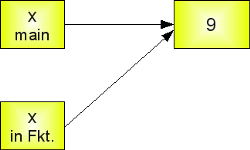
\includegraphics[width=0.7\linewidth,keepaspectratio]{boxes9}
\end{center}
        \end{column}
  \end{columns}
  
   % (Ref: https://www.python-course.eu/python3\_passing\_arguments.php)
   \end{frame}
   
 %%%%%%%%%%%%%%%%%%%%%%%%%%%%%%%%%%%%%%%%%%%%%%%%%%%%%%%%%%%%%%%%%%%%%%%%%%%%%%%%%%%
\begin{frame}[fragile]\frametitle{Python: ``Call by ??'' }
    \begin{itemize}
    \item As soon as a new value will be assigned to it, Python creates a separate local variable. 
    \item The caller's variable will not be changed this way: 
        \item After we have assigned the value 42 to x, x gets a new identity 41903752, i.e. a separate memory location from the global x. 
        \item  So, when we are back in the main scope x has still the original value 9. 
            \end{itemize}
  \begin{columns}[c]
    \begin{column}{0.5\linewidth}

            \begin{lstlisting}
            x = 9
def ref_demo(x):
    print("x=",x," id=",id(x))
    x=42
    print("x=",x," id=",id(x))
\end{lstlisting}

      \end{column}
    \begin{column}{0.4\linewidth}
    \begin{center}
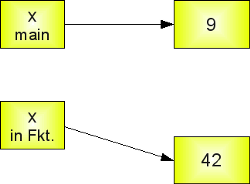
\includegraphics[width=0.7\linewidth,keepaspectratio]{boxes10}
\end{center}
        \end{column}
  \end{columns}
  
   % (Ref: https://www.python-course.eu/python3\_passing\_arguments.php)
   \end{frame}
   
    %%%%%%%%%%%%%%%%%%%%%%%%%%%%%%%%%%%%%%%%%%%%%%%%%%%%%%%%%%%%%%%%%%%%%%%%%%%%%%%%%%%
\begin{frame}[fragile]\frametitle{Python: ``Call by ??'' }

    \begin{itemize}
    \item This means that Python initially behaves like call-by-reference, but as soon as we are changing the value of such a variable, i.e. as soon as we assign a new object to it, Python "switches" to call-by-value. 
    \item This means that a local variable x will be created and the value of the global variable x will be copied into it. 
            \begin{lstlisting}
>>> x = 9
>>> id(x)
9251936
>>> ref_demo(x)
x= 9  id= 9251936
x= 42  id= 9252992
>>> id(x)
9251936
>>> 
\end{lstlisting}

            \end{itemize}
  
   (Ref: https://www.python-course.eu/python3\_passing\_arguments.php)
   \end{frame}
%
%
%
%
%
%%%%%%%%%%%%%%%%%%%%%%%%%%%%%%%%%%%%%%%%%%%%%%%%%%%%%%%%%%%%%%%%%%%%%%%%%%%%%%%%%%%%
%\begin{frame}[fragile]\frametitle{Modules}
%  The \texttt{import} statement reads a \texttt{.py} file, executes
%  it, and makes its contents available to the current program.
%\begin{lstlisting}
%>>> import re
%\end{lstlisting}
%\textbf{Modules are only read once}. Can call function multiple times.
%\begin{lstlisting}
%>>> import re
%match = re.compile(r'\d+', str)
%>>> import re
%>>> import re
%\end{lstlisting}
%
%\end{frame}
%
%%%%%%%%%%%%%%%%%%%%%%%%%%%%%%%%%%%%%%%%%%%%%%%%%%%%%%%%%%%%%%%%%%%%%%%%%%%%%%%%%%%%
%\begin{frame}[fragile]\frametitle{Modules}
%  Modules are \emph{namespaces:} 
%  Functions and variables defined in a module must be prefixed with the module name.
%
%\begin{lstlisting}
%>>> re.match(r'\d+',''Bob'')
%\end{lstlisting}
%To import definitions into the current namespace, use the
%  `\texttt{from $re$ import $match$}' form:
%\begin{lstlisting}
%>>> match(r'\d+',''Bob'')
%\end{lstlisting}
%To import ALL definitions into the current namespace, use the
%  `\texttt{from $re$ import $*$}' form:
%\end{frame}
%
%%%%%%%%%%%%%%%%%%%%%%%%%%%%%%%%%%%%%%%%%%%%%%%%%%%%%%%%%%%%%%%%%%%%%%%%%%%%%%%%%%%%
%\begin{frame}[fragile]\frametitle{The `return` statement}
%The result of a function evaluation is set by the \textit{return} statement.
%
%\begin{lstlisting}
%def double(x):
%  return x+x
%
%double(3) == 6
%\end{lstlisting}
%
%After executing \texttt{return} the control flow leaves the function.
%\begin{lstlisting}
%def double(x):
%  return x+x
%  # the following line is never exec'd
%  print('Hello')
%\end{lstlisting}
%
%
%\end{frame}
%
%%%%%%%%%%%%%%%%%%%%%%%%%%%%%%%%%%%%%%%%%%%%%%%%%%%%%%%%%%%%%%%%%%%%%%%%%%%%%%%%%%%%
%\begin{frame}[fragile]\frametitle{Globals}
%  \begin{itemize}
%  \item By default, assignment in a function or method creates local variables.
%  \item Reference (not assignment) to a variable, accesses a local variable if it has already been created, else accesses a global variable.
%  \item In order to assign a value to a global variable, declare the variable as global at the beginning of the function or method.
%  \item If in a function or method, you both reference and assign to a variable, then you must either:
%  \begin{itemize}
%  \item Assign to the variable first, or
%  \item Declare the variable as global
%    \end{itemize}
%  \end{itemize}
%\end{frame}

%%%%%%%%%%%%%%%%%%%%%%%%%%%%%%%%%%%%%%%%%%%%%%%%%%%%%%%%%%%%%%%%%%%%%%%%%%%%%%%%%%%%%
%%\begin{frame}[fragile]\frametitle{Type conversions}
%%  \begin{itemize}
%%  \item {\bf str($x$)} Converts the argument $x$ to a string; for numbers,
%%    the base 10 representation is used.
%%  \item {\bf int($x$)} Converts its argument $x$ (a number or a string) to an integer;
%%    if $x$ is a a floating-point literal, decimal digits are truncated.
%%  \item {\bf float($x$)} Converts its argument $x$ (a number or a string) to a
%%    floating-point number.
%%  \end{itemize}
%%
%%\end{frame}

%%%%%%%%%%%%%%%%%%%%%%%%%%%%%%%%%%%%%%%%%%%%%%%%%%%%%%%%%%%%%%%%%%%%%%%%%%%%%%%%%%%%%
%%\begin{frame}[fragile]  \frametitle{Special variables}
%%\begin{itemize}
%%\item Python relies on many special variables that can be accessed by your code.
%%\item One is the \lstinline{name} variables.
%%\item When a module is run, it contains the string \lstinline{main}.
%%\item When the module is imported, it contains the modules name.
%%\item You can add code that runs only when a module is called directly:\lstinline{if __name__ == __ main__: test()}
%%\end{itemize}
%%\end{frame}

% %%%%%%%%%%%%%%%%%%%%%%%%%%%%%%%%%%%%%%%%%%%%%%%%%%%%%%%%%%%%%%%%%%%%%%%%%%%%%%%%%%%
% \begin{frame}[fragile]\frametitle{lambda: anonymous functions}
% The following functions f and g do the same thing:

% \begin{lstlisting}
% def f(x): return x**2
% \end{lstlisting}

% \begin{lstlisting}
% g = lambda x: x**2
% \end{lstlisting}
% lambda functions can be place anywhere a function is expected
% without formal definition.

% \end{frame}

% %%%%%%%%%%%%%%%%%%%%%%%%%%%%%%%%%%%%%%%%%%%%%%%%%%%%%%%%%%%%%%%%%%%%%%%%%%%%%%%%%%%
% \begin{frame}[fragile]\frametitle{overloading}
% \begin{itemize}
% \item Python does not support method or function overloading. 
% \item You have to rely on the type() built-in function
% \end{itemize}
% \begin{lstlisting}
% def testtype(a):
	% if type(a) == types.FloatType:
		% print(``I got a float'')
	% elif type(A) == types.ComplexType:
		% print(``A complex number'')
	% else:
		% print(``something else'')
% \end{lstlisting}
% \end{frame}

% %%%%%%%%%%%%%%%%%%%%%%%%%%%%%%%%%%%%%%%%%%%%%%%%%%%%%%%%%%%%%%%%%%%%%%%%%%%%%%%%%%%
% \begin{frame}[fragile]\frametitle{Encrypt}
% \begin{lstlisting}
% plaintext    = list('ABCDEFGHIJKLMNOPQRSTUVWXYZ')
% encrytedtext = list('DEFGHIJKLMNOPQRSTUVWXYZABC')

% def message(text, plain, encryp):
    % dictionary = dict(zip(plain, encryp))
    % newmessage = ''
    % for char in text:
        % try:
            % newmessage += dictionary[char]
        % except:
            % newmessage += ' '
    % print(newmessage)

% message('SEND THE MATERIAL NOW')
% outputs: LTFR ZIT DQZTKOQS FGV
% \end{lstlisting}
% Write Decrypt function.
% \end{frame}

% %%%%%%%%%%%%%%%%%%%%%%%%%%%%%%%%%%%%%%%%%%%%%%%%%%%%%%%%%%%%%%%%%%%%%%%%%%%%%%%%%%%%%
% %%\begin{frame}[fragile]\frametitle{lambda}
% %%Use a lambda, as a convenience, when you need a function that both:
% %%\begin{itemize}
% %%\item is anonymous (does not need a name) and
% %%\item contains only an expression and no statements.
% %%\end{itemize}
% %%\begin{lstlisting}
% %%a = lambda x, y: (x * 3, y * 4, (x, y))
% %%a(3, 4)
% %%(9, 16, (3, 4))
% %%\end{lstlisting}
% %%\end{frame}

% %%%%%%%%%%%%%%%%%%%%%%%%%%%%%%%%%%%%%%%%%%%%%%%%%%%%%%%%%%%%%%%%%%%%%%%%%%%%%%%%%%%
% \begin{frame}[fragile]\frametitle{Iterators and generators}
% \begin{itemize}
% \item iterator: And iterator is something that satisfies the iterator protocol. Clue: If it's an iterator, you can use it in a  for:  statement.
% \item generator: A generator is a class or function that implements an iterator, i.e. that implements the iterator protocol.
% \item iterator protocol:  An object satisfies the iterator protocol if it does the following:
	% \begin{itemize}
	% \item It implements a  \lstinline|__iter__|  method, which returns an iterator object.
	% \item It implements a  \lstinline|next|  function, which returns the next item from the collection, sequence, stream, etc of items to be iterated over
	% \item It raises the  \lstinline|StopIteration|  exception when the items are exhausted and the  \lstinline|next()|  method is called.
	% \end{itemize}
% \end{itemize}

% \end{frame}

% %%%%%%%%%%%%%%%%%%%%%%%%%%%%%%%%%%%%%%%%%%%%%%%%%%%%%%%%%%%%%%%%%%%%%%%%%%%%%%%%%%%
% \begin{frame}[fragile]\frametitle{yield}
% \begin{itemize}
% \item yield: The  \lstinline{yield}  statement enables us to write functions that are generators. 
% \item The  \lstinline{yield}  statement returns a value. When the next item is requested and the iterator is ``resumed'', execution continues immediately after the  \lstinline{yield} statement.
% \item We can terminate the sequence generated by an iterator by using a  \lstinline{return} statement with no value.
% \item To resume a generator, use the generator's  \lstinline{next()}  or  \lstinline{send()}  methods. \lstinline{send()}  is like  \lstinline{next()} , but provides a value to the yield expression.
% \end{itemize}

% \begin{lstlisting}
% def list_tripler(somelist):
	% for item in somelist:
		% item *= 3
		% yield item

% it = list_tripler(alist)
	% for item in it:
		% print(item)
% \end{lstlisting}
% \end{frame}

% %%%%%%%%%%%%%%%%%%%%%%%%%%%%%%%%%%%%%%%%%%%%%%%%%%%%%%%%%%%%%%%%%%%%%%%%%%%%%%%%%%%
% \begin{frame}[fragile]\frametitle{Exercises}
% \begin{itemize}
% \item  Rewrite the grade program from the previous chapter using a function called computegrade that takes a score as its parameter and returns a grade as a
% string.
% \begin{lstlisting}
% Score Grade
% > 0.9 A
% > 0.8 B
% > 0.7 C
% > 0.6 D
% <= 0.6 F
% \end{lstlisting}
% \item Rewrite your pay computation with time-and-a-half for overtime and
% create a function called computepay which takes two parameters (hours and rate).
% \begin{lstlisting}
% Enter Hours: 45
% Enter Rate: 10
% Pay: 475.0
% \end{lstlisting}
% \end{itemize}


% \end{frame}

%%%%%%%%%%%%%%%%%%%%%%%%%%%%%%%%%%%%%%%%%%%%%%%%%%%%%%%%%%%%%%%%%%%%%%%%%%%%%%%%%%%
\begin{frame}[fragile]\frametitle{Recap (Functions)}
  \begin{itemize}
  \item Indentation is used to delimit blocks of code!
  \item Variables are just names, a reference to real object.
  \item \lstinline|def function(arg1, arg2, ...):| to define functions
  \item \lstinline|import filename| to use code from other files.
  % \item Modules are \textit{namespaces}.
  % \item Conversion between types with \lstinline|int(), float(), str()| functions.
  \item To get information on something: \lstinline|help(something)|
  \end{itemize}
\end{frame}
%%%%%%%%%%%%%%%%%%%%%%%%%%%%%%%%%%%%%%%%%%%%%%%%%%%%%%%%%%%%%%%%%%%%%%%%%%%%%%%%%%
\begin{frame}[fragile]\frametitle{}
\begin{center}
{\Large Exceptions}
\end{center}
\end{frame}


%%%%%%%%%%%%%%%%%%%%%%%%%%%%%%%%%%%%%%%%%%%%%%%%%%%%%%%%%%%%%%%%%%%%%%%%%%%%%%%%%%%
\begin{frame}[fragile]\frametitle{Exceptions}

\begin{itemize}
\item ``Exceptions'' are error conditions.
\item Code that intercepts some error conditions and
  reacts.
\item  Inherits from the built-in  Exception class.

\begin{lstlisting}
 class NewKindOfError(Exception):
    pass
 \end{lstlisting}

\item
   Exceptions are handled by class name, so they usually do not need
   any new methods (although you are free to define some if needed).

\end{itemize}
\end{frame}

%%%%%%%%%%%%%%%%%%%%%%%%%%%%%%%%%%%%%%%%%%%%%%%%%%%%%%%%%%%%%%%%%%%%%%%%%%%%%%%%%%%
\begin{frame}[fragile] \frametitle{What does an exception look like?}
\begin{lstlisting}
>>> stream.write('foo')
Traceback (most recent call last):
  File "<stdin>", line 1, in <module>
IOError: File not open for writing
\end{lstlisting}

  This is the exception \emph{message}: it is supposed to be read
  by the (human) user.
\end{frame}

%%%%%%%%%%%%%%%%%%%%%%%%%%%%%%%%%%%%%%%%%%%%%%%%%%%%%%%%%%%%%%%%%%%%%%%%%%%%%%%%%%%
\begin{frame}[fragile]\frametitle{Syntax}
\begin{lstlisting}
try:
  # code that might raise an exception
except SomeException:
  # handle some exception
except AnotherException as ex:
  # the actual Exception instance
  # is available as variable `ex'
finally:
  # performed on exit in any case
\end{lstlisting}

  The optional finally clause is executed on exit from the
  try or except block in \emph{any} case.
\end{frame}


%%%%%%%%%%%%%%%%%%%%%%%%%%%%%%%%%%%%%%%%%%%%%%%%%%%%%%%%%%%%%%%%%%%%%%%%%%%%%%%%%%%
\begin{frame}[fragile]\frametitle{Raising exceptions}

\begin{itemize}
\item   Use the raise statement with an \lstinline{Exception}
  instance:
\begin{lstlisting}
if an_error_occurred:
  raise AnError("Spider sense is tingling.")
 
\end{lstlisting}

\item The exception class name specifies what kind of exception to raise.

\item   You must use an \emph{existing} exception class; we shall learn
  how to define new exceptions in the object-orientation lectures.

\item   The exception message is an arbitrary string.  It is meant for
  humans to read, so try to describe the error condition clearly and
  concisely.
\end{itemize}

 
\end{frame}

%%%%%%%%%%%%%%%%%%%%%%%%%%%%%%%%%%%%%%%%%%%%%%%%%%%%%%%%%%%%%%%%%%%%%%%%%%%%%%%%%%%
\begin{frame}[fragile]\frametitle{Raising exceptions}
  Within an except clause, you can use raise
  with no arguments to re-raise the current exception:
\begin{lstlisting}
try:
  something()
except ItDidntWork:
  do_cleanup()
  # re-raise exception to caller
  raise
\end{lstlisting}
\end{frame}

%%%%%%%%%%%%%%%%%%%%%%%%%%%%%%%%%%%%%%%%%%%%%%%%%%%%%%%%%%%%%%%%%%%%%%%%%%%%%%%%%%%
\begin{frame}[fragile]\frametitle{raise statement}
Throw or raise an exception.
\begin{itemize}
\item Forms:
	\begin{itemize}
	\item \lstinline{raise instance}
	\item \lstinline{raise MyExceptionClass(value)}  -- preferred.
	\item \lstinline{raise MyExceptionClass, value}
	\end{itemize}
\item The  \lstinline{raise}  statement takes:
	\begin{itemize}
	\item An (instance of) a built-in exception class.
	\item An instance of class   \lstinline{Exception}  or
	\item An instance of a built-in subclass of class   \lstinline{Exception}  or
	\item An instance of a user-defined subclass of class   \lstinline{Exception}  or
	\item One of the above classes and (optionally) a value (for example, a string or a tuple).
	\end{itemize}
\end{itemize}
\end{frame}



%%%%%%%%%%%%%%%%%%%%%%%%%%%%%%%%%%%%%%%%%%%%%%%%%%%%%%%%%%%%%%%%%%%%%%%%%%%%%%%%%%%
\begin{frame}[fragile]\frametitle{Exercise}
Write a function to compute 5/0 and use try/except to catch the exceptions.
\end{frame}

%%%%%%%%%%%%%%%%%%%%%%%%%%%%%%%%%%%%%%%%%%%%%%%%%%%%%%%%%%%%%%%%%%%%%%%%%%%%%%%%%%%
\begin{frame}[fragile]\frametitle{Solution}
\begin{lstlisting}
def throws():
    return 5/0

try:
    throws()
except ZeroDivisionError:
    print "division by zero!"
except Exception as err:
    print 'Caught an exception'
finally:
    print 'In finally block for cleanup'
\end{lstlisting}
\end{frame}



%%%%%%%%%%%%%%%%%%%%%%%%%%%%%%%%%%%%%%%%%%%%%%%%%%%%%%%%%%%%%%%%%%%%%%%%%%%%%%%%%%%
\begin{frame}[fragile]\frametitle{Exercise}
Define a custom exception class which takes a string message as attribute.

Hints:

To define a custom exception, we need to define a class inherited from Exception.
\end{frame}

%%%%%%%%%%%%%%%%%%%%%%%%%%%%%%%%%%%%%%%%%%%%%%%%%%%%%%%%%%%%%%%%%%%%%%%%%%%%%%%%%%%
\begin{frame}[fragile]\frametitle{Solution}
\begin{lstlisting}
class MyError(Exception):
    """My own exception class

    Attributes:
        msg  -- explanation of the error
    """

    def __init__(self, msg):
        self.msg = msg

error = MyError("something wrong")
\end{lstlisting}
\end{frame}


% %%%%%%%%%%%%%%%%%%%%%%%%%%%%%%%%%%%%%%%%%%%%%%%%%%%%%%%%%%%%%%%%%%%%%%%%%%%%%%%%%%%
% \begin{frame}[fragile]\frametitle{Exercise}
% \begin{itemize}
% \item Enhance the function parse\_data defined in the ``Warm-up''
% \item Exercise: if an error is found in the data read from file,
    % silently ignore it and drop the line.

% \item Test your code on the
    % \href{https://raw.github.com/gc3-uzh-ch/python-course/master/rt.tsv}{\lstinline{rt.dirty.csv}}
    % data file: your code should detect and ignore the 4 malformed
    % lines in the file.
% \end{itemize}
% \end{frame}

 
\section[OOP]{Module 6: Object Oriented Programming}
%%%%%%%%%%%%%%%%%%%%%%%%%%%%%%%%%%%%%%%%%%%%%%%%%%%%%%%%%%%%%%%%%%%%%%%%%%%%%%%%%%
\begin{frame}[fragile]\frametitle{}
\begin{center}
{\Large Object-Oriented Programming: Concepts}
\end{center}
\end{frame}

%%%%%%%%%%%%%%%%%%%%%%%%%%%%%%%%%%%%%%%%%%%%%%%%%%%%%%%%%%%%%%%%%%%%%%%%%%%%%%%%%%%
\begin{frame}[fragile] \frametitle{Managing Larger Programs}
Procedural programming is:
\begin{itemize}
\item  Sequential code
\item  Conditional code (if statements)
\item  Repetitive code (loops)
\item  Store and reuse (functions)
\end{itemize}
In a very large codebase, object oriented programming is a way to arrange your code so that you
can zoom into 500 lines of the code, and understand it while ignoring the other
999,500 lines of code for the moment.
\end{frame}


%%%%%%%%%%%%%%%%%%%%%%%%%%%%%%%%%%%%%%%%%%%%%%%%%%%%%%%%%%%%%%%%%%%%%%%%%%%%%%%%%%%
\begin{frame}[fragile]\frametitle{Starting with Programs}
\begin{itemize}
\item One way to think about object oriented programming is that we are separating
our program into multiple ``zones''.
\item Each ``zone'' contains some code and data (like a program) and has well defined interactions with the outside world and the other
zones within the program.
\end{itemize}
\end{frame}

%%%%%%%%%%%%%%%%%%%%%%%%%%%%%%%%%%%%%%%%%%%%%%%%%%%%%%%%%%%%%%%%%%%%%%%%%%%%%%%%%%%
\begin{frame}[fragile]\frametitle{Sample program}
\begin{lstlisting}
import urllib.request, urllib.parse, urllib.error
from bs4 import BeautifulSoup
import ssl

# Ignore SSL certificate errors
ctx = ssl.create_default_context()
ctx.check_hostname = False
ctx.verify_mode = ssl.CERT_NONE

url = input('Enter - ')
html = urllib.request.urlopen(url, context=ctx).read()
soup = BeautifulSoup(html, 'html.parser')

# Retrieve all of the anchor tags
tags = soup('a')
for tag in tags:
	print(tag.get('href', None))
\end{lstlisting}
\end{frame}

%%%%%%%%%%%%%%%%%%%%%%%%%%%%%%%%%%%%%%%%%%%%%%%%%%%%%%%%%%%%%%%%%%%%%%%%%%%%%%%%%%%
\begin{frame}[fragile]\frametitle{Subdividing a Problem}
\begin{itemize}
\item One of the advantages of the object oriented approach is that it can hide complexity.
\item For example, while we need to know how to use the urllib and BeautifulSoup code, we do not need to know how those libraries work internally.
\item  It allows us to focus on the part of the problem we need to solve and ignore the other parts of the program.
\end{itemize}




\end{frame}


%%%%%%%%%%%%%%%%%%%%%%%%%%%%%%%%%%%%%%%%%%%%%%%%%%%%%%%%%%%%%%%%%%%%%%%%%%%%%%%%%%%
\begin{frame}[fragile]\frametitle{What's an \emph{object}?}
  \textbf{A Python object is a bundle of variables and functions.}
\begin{itemize}
\item What variable names and functions comprise an object is defined by the object's \emph{class}.

\item From one class specification, many objects can be \emph{instantiated}.  Different instances can assign different values to the object variables.

\item Variables and functions in an instance are collectively called \emph{instance attributes}; functions are also termed \emph{instance methods}.
\end{itemize}

\begin{center}
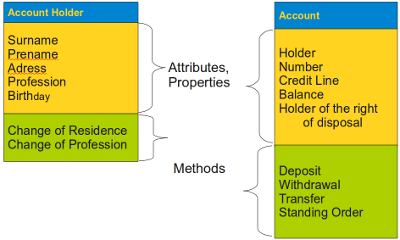
\includegraphics[width=0.5\linewidth,keepaspectratio]{oop1}
\end{center}

% (Ref: https://www.python-course.eu/object\_oriented\_programming.php)
\end{frame}

%%%%%%%%%%%%%%%%%%%%%%%%%%%%%%%%%%%%%%%%%%%%%%%%%%%%%%%%%%%%%%%%%%%%%%%%%%%%%%%%%%%
\begin{frame}[fragile]\frametitle{Encapsulation of Data}

\begin{itemize}
\item Encapsulation is the mechanism for restricting the access to some of an object's components, this means that the internal representation of an object can't be seen from outside of the objects definition. 
\item Access to this data is typically only achieved through methods
\end{itemize}

\begin{center}
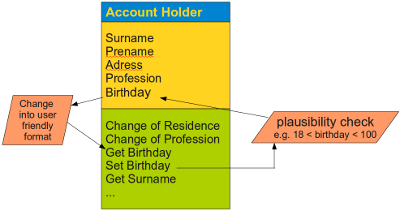
\includegraphics[width=0.5\linewidth,keepaspectratio]{oop2}
\end{center}

% (Ref: https://www.python-course.eu/object\_oriented\_programming.php)
\end{frame}

%%%%%%%%%%%%%%%%%%%%%%%%%%%%%%%%%%%%%%%%%%%%%%%%%%%%%%%%%%%%%%%%%%%%%%%%%%%%%%%%%%%
\begin{frame}[fragile]\frametitle{Inheritance}

\begin{itemize}
\item A class can inherit attributes and behaviour (methods) from other classes, called super-classes.
\item Inheritance: to create new classes by using existing classes. 
\item New ones can both be created by extending and by restricting the existing classes. 
\end{itemize}

\begin{center}
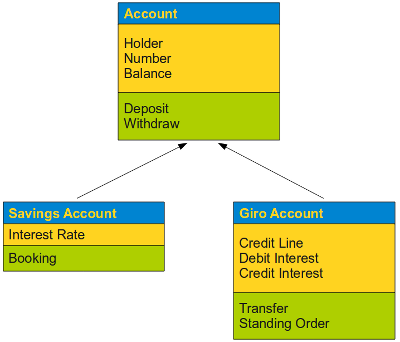
\includegraphics[width=0.5\linewidth,keepaspectratio]{oop3}
\end{center}

% (Ref: https://www.python-course.eu/object\_oriented\_programming.php)
\end{frame}


%%%%%%%%%%%%%%%%%%%%%%%%%%%%%%%%%%%%%%%%%%%%%%%%%%%%%%%%%%%%%%%%%%%%%%%%%%%%%%%%%%%
\begin{frame}[fragile]\frametitle{Using Objects}
Python provides us with many built-in objects.
\begin{lstlisting}
stuff = list()
stuff.append('python')
stuff.append('chuck')
stuff.sort()
print (stuff[0])
print (stuff.__getitem__(0))
print (list.__getitem__(stuff,0))
\end{lstlisting}
The first line is constructing an object of type list, the second and third lines are
calling the \lstinline|append()| method, the fourth line is calling the \lstinline|sort()| method, and the
fifth line is retrieving the item at position 0.
The sixth line is calling the \lstinline|__getitem__()| method in the stuff list with a parameter of zero.
\end{frame}




%%%%%%%%%%%%%%%%%%%%%%%%%%%%%%%%%%%%%%%%%%%%%%%%%%%%%%%%%%%%%%%%%%%%%%%%%%%%%%%%%%%
\begin{frame}[fragile]\frametitle{Example}
Import the \lstinline{date} class from the standard library module \lstinline{datetime}
\begin{lstlisting}
>>> from datetime import date
>>> dt1 = date(2012, 9, 28)
>>> dt2 = date(2012, 10, 1)
\end{lstlisting}
To instantiate an object, call the class name like a function.
\begin{lstlisting}
>>> from datetime import date
>>> dt1 = date(2012, 9, 28)
>>> dt2 = date(2012, 10, 1)
\end{lstlisting}
\end{frame}

%%%%%%%%%%%%%%%%%%%%%%%%%%%%%%%%%%%%%%%%%%%%%%%%%%%%%%%%%%%%%%%%%%%%%%%%%%%%%%%%%%%
\begin{frame}[fragile] \frametitle{Example}
\begin{lstlisting}
>>> dir(dt1)
['__add__', '__class__', 'ctime', 'day',
'fromordinal', 'fromtimestamp', 'isocalendar',
'isoformat', 'isoweekday', 'max', 'min', 'month',
'replace', 'resolution', 'strftime', 'timetuple',
'today', 'toordinal', 'weekday', 'year']
\end{lstlisting}
The \lstinline{dir} function can list all objects attributes. Note there is no distinction between instance variables and methods! Access to object attributes is done by suffixing the instance name with the attribute name, separated by a dot ``\lstinline{.}''.
\begin{lstlisting}
>>> dt1.day
28
>>> dt1.month
9
>>> dt1.year
2012
\end{lstlisting}
\end{frame}

%%%%%%%%%%%%%%%%%%%%%%%%%%%%%%%%%%%%%%%%%%%%%%%%%%%%%%%%%%%%%%%%%%%%%%%%%%%%%%%%%%%
\begin{frame}[fragile]\frametitle{Starting with OOP}
\begin{lstlisting}
class PartyAnimal:
	x = 0
	def party(self) :
		self.x = self.x + 1
		print("So far",self.x)

an = PartyAnimal()
an.party()
an.party()
an.party()
PartyAnimal.party(an)
\end{lstlisting}
When the party method is called, the first parameter (self) points to the particular instance of the PartyAnimal object that party is called from within. 
Within the party method, we see the line:
\lstinline|self.x = self.x + 1|
\end{frame}

%%%%%%%%%%%%%%%%%%%%%%%%%%%%%%%%%%%%%%%%%%%%%%%%%%%%%%%%%%%%%%%%%%%%%%%%%%%%%%%%%%%
\begin{frame}[fragile]\frametitle{Starting with OOP}
Following line is another way to call the party method within
the an object: \lstinline|PartyAnimal.party(an)|
When the program executes, it produces the following output:
\begin{lstlisting}
So far 1
So far 2
So far 3
So far 4
\end{lstlisting}
\end{frame}


%%%%%%%%%%%%%%%%%%%%%%%%%%%%%%%%%%%%%%%%%%%%%%%%%%%%%%%%%%%%%%%%%%%%%%%%%%%%%%%%%%%
\begin{frame}[fragile]\frametitle{The \texttt{self} argument}

  \textbf{Every method of a Python object always has \texttt{self}
    as first argument.}

  
  However, you do not specify it when calling a method: it's
  automatically inserted by Python:
\begin{lstlisting}
>>> class ShowSelf(object):
...   def show(self):
...     print(self)
...
>>> x = ShowSelf() # construct instance
>>> x.show() # `self' automatically inserted!
<__main__.ShowSelf object at 0x299e150>
\end{lstlisting}

  
  The \texttt{self} name is a reference to the object instance
  itself.  You \emph{need to} use \texttt{self} when accessing methods
  or attributes of this instance.
\end{frame}

%%%%%%%%%%%%%%%%%%%%%%%%%%%%%%%%%%%%%%%%%%%%%%%%%%%%%%%%%%%%%%%%%%%%%%%%%%%%%%%%%%%
\begin{frame}[fragile]\frametitle{Member functions}
There are different types of methods/functions.
\begin{lstlisting}
class MyClass:
    def method(self):
        return 'instance method called', self

    @classmethod
    def classmethod(cls):
        return 'class method called', cls

    @staticmethod
    def staticmethod():
        return 'static method called'
\end{lstlisting}
Instead of using a plain class MyClass: declaration you may choose to declare a new-style class inheriting from object with the class MyClass(object):
\end{frame}


%%%%%%%%%%%%%%%%%%%%%%%%%%%%%%%%%%%%%%%%%%%%%%%%%%%%%%%%%%%%%%%%%%%%%%%%%%%%%%%%%%%
\begin{frame}[fragile]\frametitle{Member functions: Instance Methods}

\begin{lstlisting}
class MyClass:
    def method(self):
        return 'instance method called', self
\end{lstlisting}
Through the self parameter, instance methods can freely access attributes and other methods on the same object. 

% (Ref: https://realpython.com/blog/python/instance-class-and-static-methods-demystified/)
\end{frame}


%%%%%%%%%%%%%%%%%%%%%%%%%%%%%%%%%%%%%%%%%%%%%%%%%%%%%%%%%%%%%%%%%%%%%%%%%%%%%%%%%%%
\begin{frame}[fragile]\frametitle{Member functions: Class Methods}
This method is with a @classmethod decorator to flag it as a class method.
\begin{lstlisting}
class MyClass:
    @classmethod
    def classmethod(cls):
        return 'class method called', cls

\end{lstlisting}
  \begin{itemize}
  \item Instead of accepting a self parameter, class methods take a cls parameter that points to the class-and not the object instance-when the method is called.
  \item Because the class method only has access to this cls argument, it can't modify object instance state. 
    \item That would require access to self. However, class methods can still modify class state that applies across all instances of the class.
  \end{itemize}
  
% (Ref: https://realpython.com/blog/python/instance-class-and-static-methods-demystified/)
\end{frame}

%%%%%%%%%%%%%%%%%%%%%%%%%%%%%%%%%%%%%%%%%%%%%%%%%%%%%%%%%%%%%%%%%%%%%%%%%%%%%%%%%%%
\begin{frame}[fragile]\frametitle{Member functions: Static Methods}
Marked with a @staticmethod decorator to flag it as a static method.
\begin{lstlisting}
class MyClass:
    @staticmethod
    def staticmethod():
        return 'static method called'

\end{lstlisting}
  \begin{itemize}
  \item This type of method takes neither a self nor a cls parameter (but of course it's free to accept an arbitrary number of other parameters).
  \item Therefore a static method can neither modify object state nor class state. Static methods are restricted in what data they can access - and they're primarily a way to namespace your methods.
  \end{itemize}
  
% (Ref: https://realpython.com/blog/python/instance-class-and-static-methods-demystified/)
\end{frame}


%%%%%%%%%%%%%%%%%%%%%%%%%%%%%%%%%%%%%%%%%%%%%%%%%%%%%%%%%%%%%%%%%%%%%%%%%%%%%%%%%%%
\begin{frame}[fragile]\frametitle{Member functions: Instance Methods}

\begin{lstlisting}
>>> obj = MyClass()
>>> obj.method()
('instance method called', <MyClass instance at 0x101a2f4c8>)
\end{lstlisting}
This confirmed that method (the instance method) has access to the object instance (printed as ``MyClass instance'') via the self argument.
When the method is called, Python replaces the self argument with the instance object, obj. 

% (Ref: https://realpython.com/blog/python/instance-class-and-static-methods-demystified/)
\end{frame}

%%%%%%%%%%%%%%%%%%%%%%%%%%%%%%%%%%%%%%%%%%%%%%%%%%%%%%%%%%%%%%%%%%%%%%%%%%%%%%%%%%%
\begin{frame}[fragile]\frametitle{Member functions: Instance Methods}

We could ignore the syntactic sugar of the dot-call syntax (obj.method()) and pass the instance object manually to get the same result:

\begin{lstlisting}
>>> MyClass.method(obj)
('instance method called', <MyClass instance at 0x101a2f4c8>)
\end{lstlisting}

% (Ref: https://realpython.com/blog/python/instance-class-and-static-methods-demystified/)
\end{frame}

%%%%%%%%%%%%%%%%%%%%%%%%%%%%%%%%%%%%%%%%%%%%%%%%%%%%%%%%%%%%%%%%%%%%%%%%%%%%%%%%%%%
\begin{frame}[fragile]\frametitle{Member functions: Class Methods}

\begin{lstlisting}
>>> obj.classmethod()
('class method called', <class MyClass at 0x101a2f4c8>)
\end{lstlisting}

  \begin{itemize}
  \item Calling classmethod() showed us it doesn't have access to the ``MyClass instance'' object, but only to the ``class MyClass'' object, representing the class itself (everything in Python is an object, even classes themselves).

  \item Please note that naming these parameters self and cls is just a convention. You could just as easily name them the\_object and the\_class and get the same result. 
  \end{itemize}
  
% (Ref: https://realpython.com/blog/python/instance-class-and-static-methods-demystified/)
\end{frame}

%%%%%%%%%%%%%%%%%%%%%%%%%%%%%%%%%%%%%%%%%%%%%%%%%%%%%%%%%%%%%%%%%%%%%%%%%%%%%%%%%%%
\begin{frame}[fragile]\frametitle{Member functions: Static Methods}

\begin{lstlisting}
>>> obj.staticmethod()
'static method called'
\end{lstlisting}

  \begin{itemize}
  \item Aren't we surprised when they learn that it's possible to call a static method on an object instance.
  \item Behind the scenes Python simply enforces the access restrictions by not passing in the self or the cls argument when a static method gets called using the dot syntax.
  \item This confirms that static methods can neither access the object instance state nor the class state. 
  \item They work like regular functions but belong to the class's (and every instance's) namespace.
  \end{itemize}
% (Ref: https://realpython.com/blog/python/instance-class-and-static-methods-demystified/)
\end{frame}


%%%%%%%%%%%%%%%%%%%%%%%%%%%%%%%%%%%%%%%%%%%%%%%%%%%%%%%%%%%%%%%%%%%%%%%%%%%%%%%%%%%
\begin{frame}[fragile]\frametitle{Member functions: Cases}
When we attempt to call these methods on the class itself - without creating an object instance beforehand:
\begin{lstlisting}
>>> MyClass.classmethod()
('class method called', <class MyClass at 0x101a2f4c8>)

>>> MyClass.staticmethod()
'static method called'

>>> MyClass.method()
TypeError: unbound method method() must
    be called with MyClass instance as first
    argument (got nothing instead)
\end{lstlisting}

  \begin{itemize}
  \item We didn't create an object instance and tried calling an instance function directly on the class blueprint itself. 
  \item This means there is no way for Python to populate the self argument and therefore the call fails.
  \end{itemize}
% (Ref: https://realpython.com/blog/python/instance-class-and-static-methods-demystified/)
\end{frame}

%%%%%%%%%%%%%%%%%%%%%%%%%%%%%%%%%%%%%%%%%%%%%%%%%%%%%%%%%%%%%%%%%%%%%%%%%%%%%%%%%%%
\begin{frame}[fragile]\frametitle{Member functions: Why Static methods?}

\begin{lstlisting}
import math

class Pizza:
    def __init__(self, radius, ingredients):
        self.radius = radius
        self.ingredients = ingredients

    def __repr__(self):
        return (f'Pizza({self.radius!r}, '
                f'{self.ingredients!r})')

    def area(self):
        return self.circle_area(self.radius)

    @staticmethod
    def circle_area(r):
        return r ** 2 * math.pi
\end{lstlisting}

Instead of calculating the area directly within area(), using the well-known circle area formula, I factored that out to a separate circle\_area() static method.

% (Ref: https://realpython.com/blog/python/instance-class-and-static-methods-demystified/)
\end{frame}


%%%%%%%%%%%%%%%%%%%%%%%%%%%%%%%%%%%%%%%%%%%%%%%%%%%%%%%%%%%%%%%%%%%%%%%%%%%%%%%%%%%
\begin{frame}[fragile]\frametitle{Member functions: Why Static methods?}
   \begin{itemize}
  \item As don't take a cls or self argument. That's a big limitation- but it's also a great signal to show that a particular method is independent from everything else around it.
	\item Now, why is that useful?
	\item Flagging a method as a static method is not just a hint that a method won't modify class or instance state - this restriction is also enforced by the Python runtime.
	\item Techniques like that allow you to communicate clearly the intention.
  \end{itemize}

% (Ref: https://realpython.com/blog/python/instance-class-and-static-methods-demystified/)
\end{frame}


%%%%%%%%%%%%%%%%%%%%%%%%%%%%%%%%%%%%%%%%%%%%%%%%%%%%%%%%%%%%%%%%%%%%%%%%%%%%%%%%%%%
\begin{frame}[fragile]\frametitle{Member functions: Properties}
getters and setters:
\begin{lstlisting}
class TestProperty(object):
    def __init__(self, description):
        self._description = description
    @property
    def description(self):
        print 'getting description'
        return self._description
    @description.setter
    def description(self, description):
        print 'setting description'
        self._description = description
\end{lstlisting}
We mark the instance variable as private by prefixing it with an underscore.

The name of the instance variable and the name of the property must be different. If they are not, we get recursion and an error.
\end{frame}

%%%%%%%%%%%%%%%%%%%%%%%%%%%%%%%%%%%%%%%%%%%%%%%%%%%%%%%%%%%%%%%%%%%%%%%%%%%%%%%%%%%
\begin{frame}[fragile]\frametitle{Member function: \_\_init\_\_}
   \begin{itemize}
  \item ``\_\_init\_\_'' is a reseved method in python classes. 
  \item Python doesn't have explicit constructors like C++ or Java, but the \_\_init\_\_() method in Python is something similar, though it is strictly speaking not a constructor. 
  \item It behaves in many ways like a constructor, e.g. it is the first code which is executed, when a new instance of a class is created.
   \end{itemize}
   
\begin{lstlisting}
class Car(object):
	def __init__(self, model, color, company, speed_limit):
		self.color = color
		self.company = company
		self.speed_limit = speed_limit
		self.model = model

\end{lstlisting}

% (Ref: https://micropyramid.com/blog/understand-self-and-\_\_init\_\_-method-in-python-class/)
\end{frame}

%%%%%%%%%%%%%%%%%%%%%%%%%%%%%%%%%%%%%%%%%%%%%%%%%%%%%%%%%%%%%%%%%%%%%%%%%%%%%%%%%%%
\begin{frame}[fragile]\frametitle{Member function: Destructor}
   \begin{itemize}
  \item There is no "real" destructor, but something similiar, i.e. the method \_\_del\_\_. 
  \item It is called when the instance is about to be destroyed. 
  \item If a base class has a \_\_del\_\_() method, the derived class's \_\_del\_\_() method, if any, must explicitly call it to ensure proper deletion of the base class part of the instance. 
   \end{itemize}
   
   
\begin{lstlisting}
class Greeting:
    def __init__(self, name):
        self.name = name
    def __del__(self):
        print "Destructor started"
    def SayHello(self):
        print "Hello", self.name

\end{lstlisting}   
\end{frame}

%%%%%%%%%%%%%%%%%%%%%%%%%%%%%%%%%%%%%%%%%%%%%%%%%%%%%%%%%%%%%%%%%%%%%%%%%%%%%%%%%%%
\begin{frame}[fragile]\frametitle{Member function: Example Construction Destruction}
   
\begin{lstlisting}
>>> from hello_class import Greeting
>>> x1 = Greeting("Guido")
>>> x2 = x1
>>> del x1
>>> del x2
Destructor started   
\end{lstlisting}
   \begin{itemize}
  \item If we use this class, we can see, the "del" doesn't directly call the \_\_del\_\_() method. 
  \item It's apparent that the destructor is not called, when we delete x1. 
  \item The reason is that del decrements the reference count for the object of x1 by one. 
  \item Only if the reference count reaches zero, the destructor is called
     \end{itemize}
\end{frame}



%%%%%%%%%%%%%%%%%%%%%%%%%%%%%%%%%%%%%%%%%%%%%%%%%%%%%%%%%%%%%%%%%%%%%%%%%%%%%%%%%%%
\begin{frame}
  \frametitle{No access control}
  There are no ``public'', ``private'' and 'protected''. qualifiers for object
  attributes.

  
  \textbf{\emph{Any} code can create/read/overwrite/delete \emph{any} attribute on
    \emph{any} object.}

  
  There are \emph{conventions}, though:
  \begin{itemize}
  \item ``protected'' attributes: \texttt{\_name\_}
  \item ``private'' attributes: \texttt{\_\_name\_\_}
  \end{itemize}
  (But again, note that this is not \emph{enforced} by the system in
  any way.)

\end{frame}

%%%%%%%%%%%%%%%%%%%%%%%%%%%%%%%%%%%%%%%%%%%%%%%%%%%%%%%%%%%%%%%%%%%%%%%%%%%%%%%%%%%
 \begin{frame}\frametitle{No overloading}

\begin{itemize}
\item Python does not allow overloading of functions.
\item Any function.
\item Hence, no overloading of constructors.
\item So: \textbf{a class has one and only one constructor.}
\end{itemize}
 \end{frame}


%%%%%%%%%%%%%%%%%%%%%%%%%%%%%%%%%%%%%%%%%%%%%%%%%%%%%%%%%%%%%%%%%%%%%%%%%%%%%%%%%%%
\begin{frame}[fragile]\frametitle{Constructor chaining}
  % \begin{flushright}
  %   \footnotesize%
  %   {\em ``Explicit is better than implicit''}
  %   --- T.~Peters, \href{http://www.python.org/dev/peps/pep-0020/}{The
  %     Zen of Python}
  % \end{flushright}

    When a class is instantiated, Python only calls the first
    constructor it can find in the
    \href{http://www.python.org/download/releases/2.3/mro/}{class inheritance call-chain}.

    %\+ 
    \textbf{If you need to call a parent constructor, you need
      to do it \emph{explicitly}:}
    \begin{lstlisting}
class Application(Task):
  def __init__(self, ...):
    # do Application-specific stuff here
    Task.__init__(self, ...)
    # some more Application-specific stuff
    \end{lstlisting}

    %\+
    Calling a superclass constructor is optional, and
    it can happen anywhere in the init method body.
\end{frame}


%%%%%%%%%%%%%%%%%%%%%%%%%%%%%%%%%%%%%%%%%%%%%%%%%%%%%%%%%%%%%%%%%%%%%%%%%%%%%%%%%%%
\begin{frame}[fragile]\frametitle{Classes as Types}
All variables have a type. And we can use the built-in
dir function to examine the capabilities of a variable. We can use type and dir
with the classes that we create.
\begin{lstlisting}
class PartyAnimal:
	x = 0
	def party(self) :
		self.x = self.x + 1
		print("So far",self.x)

an = PartyAnimal()
print ("Type", type(an))
print ("Dir ", dir(an))
print ("Type", type(an.x))
print ("Type", type(an.party))
\end{lstlisting}
\end{frame}

%%%%%%%%%%%%%%%%%%%%%%%%%%%%%%%%%%%%%%%%%%%%%%%%%%%%%%%%%%%%%%%%%%%%%%%%%%%%%%%%%%%
\begin{frame}[fragile]\frametitle{Object Life-cycle}
As our objects become more complex, we need to take some action within the object to set things up as
the object is being constructed and possibly clean things up as the object is being
discarded.
\begin{lstlisting}
class PartyAnimal:
	x = 0
	def __init__(self):
		print('I am constructed')
	
	def party(self) :
		self.x = self.x + 1
		print('So far',self.x)

	def __del__(self):
		print('I am destructed', self.x)

an = PartyAnimal()
an.party()
an.party()
an = 42
print('an contains',an)
\end{lstlisting}
\end{frame}

%%%%%%%%%%%%%%%%%%%%%%%%%%%%%%%%%%%%%%%%%%%%%%%%%%%%%%%%%%%%%%%%%%%%%%%%%%%%%%%%%%%
\begin{frame}[fragile]\frametitle{Many Instances}
When we are making multiple objects from our class, we might want to set up different initial values for each of the objects.
\begin{lstlisting}
class PartyAnimal:
	x = 0
	name = ''
	def __init__(self, nam):
		self.name = nam
		print(self.name,'constructed')

	def party(self) :
		self.x = self.x + 1
		print(self.name,'party count',self.x)

s = PartyAnimal('Sally')
s.party()
j = PartyAnimal('Jim')
j.party()
s.party()
\end{lstlisting}
\end{frame}

%%%%%%%%%%%%%%%%%%%%%%%%%%%%%%%%%%%%%%%%%%%%%%%%%%%%%%%%%%%%%%%%%%%%%%%%%%%%%%%%%%%
\begin{frame}[fragile]\frametitle{Inheritance}
Ability to create a new class by extending an existing class. When extending a class, we call the
original class the 'parent class' (object) and the new class as the 'child class' (PartyAnimal).
\begin{lstlisting}
class PartyAnimal(object):
	x = 0
	name = ''
	def __init__(self, nam):
		self.name = nam
		print(self.name,'constructed')

	def party(self) :
		self.x = self.x + 1
		print(self.name,'party count',self.x)
\end{lstlisting}
\end{frame}


%%%%%%%%%%%%%%%%%%%%%%%%%%%%%%%%%%%%%%%%%%%%%%%%%%%%%%%%%%%%%%%%%%%%%%%%%%%%%%%%%%%
\begin{frame}[fragile]\frametitle{Child Class}
We can `import' the PartyAnimal class in a new file and extend it as follows:
\begin{lstlisting}
from party import PartyAnimal

class CricketFan(PartyAnimal):
	points = 0

	def six(self):
		self.points = self.points + 6
		self.party()
		print(self.name,"points",self.points)

s = PartyAnimal("Sally")
s.party()
j = CricketFan("Jim")
j.party()
j.six()
print(dir(j))	
\end{lstlisting}
\end{frame}

%%%%%%%%%%%%%%%%%%%%%%%%%%%%%%%%%%%%%%%%%%%%%%%%%%%%%%%%%%%%%%%%%%%%%%%%%%%%%%%%%%%
\begin{frame}[fragile]\frametitle{Inheritance: Try}

\begin{lstlisting}
class Vehicle:
    def __init__(self, name, color):
        self.__name = name      # __name is private to Vehicle class
        self.__color = color
    def getColor(self):         # getColor() function is accessible to class Car
        return self.__color
    def setColor(self, color):  # setColor is accessible outside the class
        self.__color = color
    def getName(self):          # getName() is accessible outside the class
        return self.__name
 
\end{lstlisting}
\end{frame}

%%%%%%%%%%%%%%%%%%%%%%%%%%%%%%%%%%%%%%%%%%%%%%%%%%%%%%%%%%%%%%%%%%%%%%%%%%%%%%%%%%%
\begin{frame}[fragile]\frametitle{Inheritance: Try}

\begin{lstlisting}
class Car(Vehicle):
    def __init__(self, name, color, model):
        # call parent constructor to set name and color  
        super().__init__(name, color)       
        self.__model = model
    def getDescription(self):
        return self.getName() + self.__model + " in " + self.getColor() + " color"
 
# in method getDescrition we are able to call getName(), getColor() because they are 
# accessible to child class through inheritance
c = Car("Ford Mustang", "red", "GT350")
print(c.getDescription())
print(c.getName()) # car has no method getName() but it is accessible through class Vehicle
\end{lstlisting}
\end{frame}



%%%%%%%%%%%%%%%%%%%%%%%%%%%%%%%%%%%%%%%%%%%%%%%%%%%%%%%%%%%%%%%%%%%%%%%%%%%%%%%%%%%
\begin{frame}[fragile]\frametitle{Multiple Inheritance}

A class can inherit from more than one class. 
\begin{lstlisting}
class MySuperClass1():
 
    def method_super1(self):
        print("method_super1 method called")
 
class MySuperClass2():
 
    def method_super2(self):
        print("method_super2 method called")
 
class ChildClass(MySuperClass1, MySuperClass2):
 
    def child_method(self):
        print("child method")
 
c = ChildClass()
c.method_super1()
c.method_super2()
\end{lstlisting}
\end{frame}

%%%%%%%%%%%%%%%%%%%%%%%%%%%%%%%%%%%%%%%%%%%%%%%%%%%%%%%%%%%%%%%%%%%%%%%%%%%%%%%%%%%
\begin{frame}[fragile]\frametitle{Overriding methods}
To override a method in the base class, sub class needs to define a method of same signature. (i.e same method name and same number of parameters as method in base class).

\begin{lstlisting}
class A():
    def __init__(self):
        self.__x = 1
    def m1(self):
        print("m1 from A")
 
class B(A):
    def __init__(self):
        self.__y = 1
    def m1(self):
        print("m1 from B")
 
c = B()
c.m1() # m1 from B
\end{lstlisting}
Try commenting m1()  method  in B  class and now m1()  method from Base class i.e class A  will run.
\end{frame}


%%%%%%%%%%%%%%%%%%%%%%%%%%%%%%%%%%%%%%%%%%%%%%%%%%%%%%%%%%%%%%%%%%%%%%%%%%%%%%%%%%%
\begin{frame}[fragile]\frametitle{isinstance() function}

Used to determine whether the object is an instance of the class or not.
\begin{lstlisting}
>>> isinstance(1, int)
True
 
>>> isinstance(1.2, int)
False
 
>>> isinstance([1,2,3,4], list)
True
\end{lstlisting}

\end{frame}

%%%%%%%%%%%%%%%%%%%%%%%%%%%%%%%%%%%%%%%%%%%%%%%%%%%%%%%%%%%%%%%%%%%%%%%%%%%%%%%%%%%%
%\begin{frame}[fragile] \frametitle{First class objects}
%\begin{itemize}
%\item  All objects in Python are first class. In short, it means there are no restrictions on the object's use. It's the same as any other object.
%\item  Definition, An object is first class if: 
%	\begin{itemize}
%	\item Can be dynamically created, destroyed, 
%	\item passed to a function, returned as a value
%	\end{itemize}
%\item References -- Objects (or references to them) can be shared.  What does this mean?
%	\begin{itemize}
%	\item The object(s) satisfy the identity test operator \lstinline{is}.
%	\item The built-in function \lstinline{id()} returns the same value.
%	\item \lstinline|del()|  -- The built-in function  \lstinline|del()|  removes a reference, not (necessarily)
%the object itself.
%	\end{itemize}
%\end{itemize}
%\end{frame}

%%%%%%%%%%%%%%%%%%%%%%%%%%%%%%%%%%%%%%%%%%%%%%%%%%%%%%%%%%%%%%%%%%%%%%%%%%%%%%%%%%%
\begin{frame}[fragile] \frametitle{Inspection}
\begin{itemize}
\item  Learn what the type of an object is -- Example:  \lstinline|type(obj)|
\item Learn what attributes an object has and what it's capabilities are -- Example: \lstinline|dir(obj)|
\item Get help on a class or an object -- Example:  \lstinline|help(obj)|
\item In Ipython:\lstinline| In [49]: a.upper?|
\end{itemize}
\end{frame}


%%%%%%%%%%%%%%%%%%%%%%%%%%%%%%%%%%%%%%%%%%%%%%%%%%%%%%%%%%%%%%%%%%%%%%%%%%%%%%%%%%%
\begin{frame}[fragile]\frametitle{Exercise}
\begin{itemize}
\item Define a class which has at least two methods:
\item getString: to get a string from console input
\item printString: to print the string in upper case.
\item Also please include simple test function to test the class methods.
\item Hints: Use \_\_init\_\_ method to construct some parameters
\end{itemize}
\end{frame}

%%%%%%%%%%%%%%%%%%%%%%%%%%%%%%%%%%%%%%%%%%%%%%%%%%%%%%%%%%%%%%%%%%%%%%%%%%%%%%%%%%%
\begin{frame}[fragile]\frametitle{Solution}
\begin{lstlisting}
class InputOutString(object):
    def __init__(self):
        self.s = ""

    def getString(self):
        self.s = input()

    def printString(self):
        print self.s.upper()

strObj = InputOutString()
strObj.getString()
strObj.printString()
\end{lstlisting}
\end{frame}

%%%%%%%%%%%%%%%%%%%%%%%%%%%%%%%%%%%%%%%%%%%%%%%%%%%%%%%%%%%%%%%%%%%%%%%%%%%%%%%%%%
\begin{frame}[fragile]\frametitle{}
\begin{center}
{\Large Object Oriented Programming: Examples}
\end{center}
\end{frame}


%%%%%%%%%%%%%%%%%%%%%%%%%%%%%%%%%%%%%%%%%%%%%%%%%%%%%%%%%%%%%%%%%%%%%%%%%%%%%%%%%%%
\begin{frame}[fragile]\frametitle{Recall: \emph{What is a 2D vector?}}

\begin{itemize}
\item A \emph{2D} vector is an element of the vector space $\mathbb{R}^2$.
\item Every \emph{2D} vector $\mathbf{u}$ is completely described by a
  pair of real coordinates $\langle u_x, u_y \rangle$.
\item Note: It is not a point in space. It gives Direction, like a movement recipe. 
\item When added to a point, results into a transformed point.
\end{itemize}
  
  
  
  Two operations are defined on vectors:

  
  \begin{columns}
    \begin{column}{0.6\linewidth}
      \raggedleft
      \emph{vector addition:} if $\mathbf{w} = \mathbf{u} +
        \mathbf{v}$, then $w_x = u_x + v_x$ and $w_y = u_y + v_y$.
    \end{column}
    \begin{column}{0.4\linewidth}
      \centering
      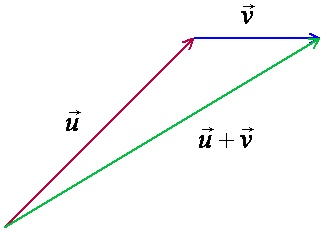
\includegraphics[height=4\baselineskip]{VectorAddition.jpg}
    \end{column}
  \end{columns}

  
  \begin{columns}
    \begin{column}{0.4\linewidth}
      \centering
      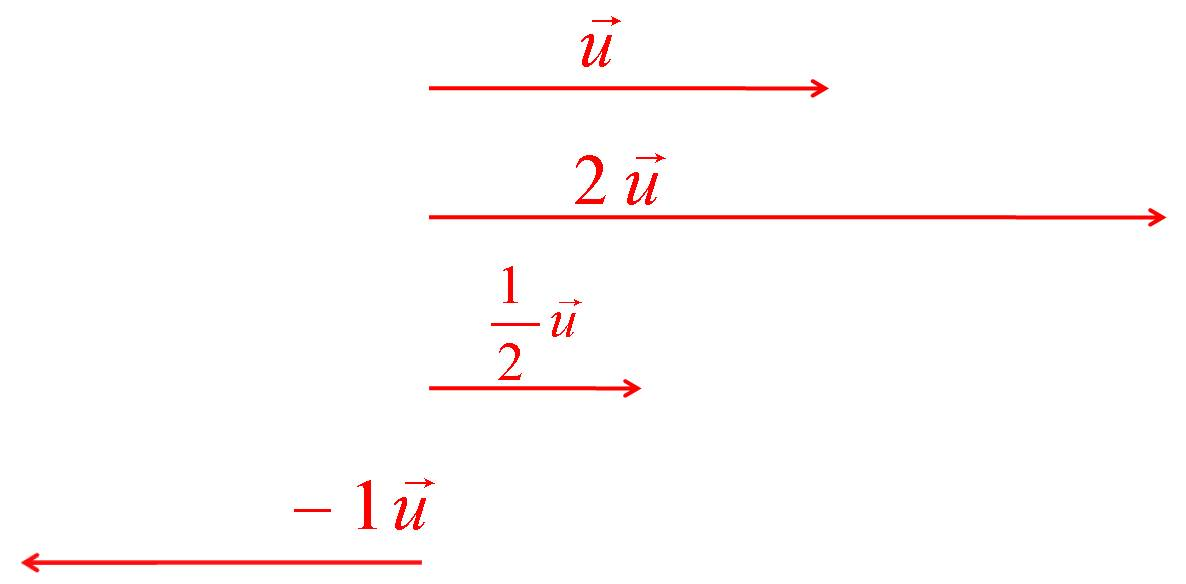
\includegraphics[height=3\baselineskip]{VectorScalarMultiplication.jpg}
    \end{column}
    \begin{column}{0.6\linewidth}
      \raggedright
      \emph{scalar multiplication:} if $\mathbf{v} = \alpha
      \cdot \mathbf{u}$ with $\alpha \in \mathbb{R}$, then $v_x =
      \alpha \cdot u_x$ and $v_y = \alpha \cdot u_y$.
    \end{column}
  \end{columns}

\end{frame}

%%%%%%%%%%%%%%%%%%%%%%%%%%%%%%%%%%%%%%%%%%%%%%%%%%%%%%%%%%%%%%%%%%%%%%%%%%%%%%%%%%%
\begin{frame}[fragile]\frametitle{A \emph{2D vector} in Python}
\begin{lstlisting}
class Vector(object):
 
  def __init__(self, x, y):
    self.x = x
    self.y = y
    
  def add(self, other):
    return Vector(self.x+other.x,
                  self.y+other.y)
                  
  def mul(self, scalar):
    return Vector(scalar*self.x, scalar*self.y)
    
  def show(self):
    return (''<{},{}>''.format(self.x, self.y))
    
\end{lstlisting}
\end{frame}


%%%%%%%%%%%%%%%%%%%%%%%%%%%%%%%%%%%%%%%%%%%%%%%%%%%%%%%%%%%%%%%%%%%%%%%%%%%%%%%%%%%%
%\begin{frame}[fragile]\frametitle{Operations}
%      This identifies user-defined~classes.
%      (Do not leave it out or you'll get an ``old-style'' class, which
%      is deprecated behavior.)
%\begin{lstlisting}
%class Vector(object):
%  """A 2D Vector."""
%  def __init__(self, x, y):
%    self.x = x
%    self.y = y
%  def add(self, other):
%    return Vector(self.x+other.x,
%                  self.y+other.y)
%  def mul(self, scalar):
%    return Vector(scalar*self.x, scalar*self.y)
%  def show(self):
%    return ("<\%g,\%g>" \% (self.x, self.y))
%\end{lstlisting}
%\end{frame}

%%%%%%%%%%%%%%%%%%%%%%%%%%%%%%%%%%%%%%%%%%%%%%%%%%%%%%%%%%%%%%%%%%%%%%%%%%%%%%%%%%%
\begin{frame}[fragile]\frametitle{DocString}
      Classes can have docstrings.
      The content of a class docstring will be shown as help text for
      that class.
\begin{lstlisting}
class Vector(object):
  """A 2D Vector."""
  def __init__(self, x, y):
    self.x = x
    self.y = y
  def add(self, other):
    return Vector(self.x+other.x,
                  self.y+other.y)
  def mul(self, scalar):
    return Vector(scalar*self.x, scalar*self.y)
  def show(self):
    return (''<{},{}>''.format(self.x, self.y))
\end{lstlisting}

\end{frame}


%%%%%%%%%%%%%%%%%%%%%%%%%%%%%%%%%%%%%%%%%%%%%%%%%%%%%%%%%%%%%%%%%%%%%%%%%%%%%%%%%%%
\begin{frame}[fragile]\frametitle{Member functions}
%  \begin{columns}[t]
%    \begin{column}{0.5\linewidth}
\begin{lstlisting}
class Vector(object):
  """A 2D Vector."""
  def __init__(self, x, y):
    self.x = x
    self.y = y
  def add(self, other):
    return Vector(self.x+other.x,
                  self.y+other.y)
  def mul(self, scalar):
    return Vector(scalar*self.x, scalar*self.y)
  def show(self):
    return (''<{},{}>''.format(self.x, self.y))
\end{lstlisting}
%    \end{column}
%    \begin{column}{0.5\linewidth}
%      \raggedleft
      The {\bf def} keyword introduces a method~definition.

      
      Every method \emph{must} have at~least one argument,
      named~{\bf self}.
%    \end{column}
%  \end{columns}
\end{frame}

%%%%%%%%%%%%%%%%%%%%%%%%%%%%%%%%%%%%%%%%%%%%%%%%%%%%%%%%%%%%%%%%%%%%%%%%%%%%%%%%%%%
\begin{frame}[fragile]\frametitle{Exercises}
\begin{itemize}
\item Add a new method \texttt{norm} the \texttt{Vector} class: if
    \texttt{v} is an instance of class \texttt{Vector}, then calling
    \texttt{v.norm()} returns the norm $\sqrt{v_x^2 + v_y^2}$ of
    the associated vector.
\item 
    Add a new method \texttt{unit} to the \texttt{Vector} class: if
    \texttt{v} is an instance of class \texttt{Vector}, then calling
    \texttt{v.unit()} returns the vector \texttt{u} having the
    same direction as \texttt{v} but norm $1$.
\end{itemize}
\end{frame}


%%%%%%%%%%%%%%%%%%%%%%%%%%%%%%%%%%%%%%%%%%%%%%%%%%%%%%%%%%%%%%%%%%%%%%%%%%%%%%%%%%%%
%\begin{frame}[fragile]\frametitle{Recall: 2D Vector}
%  \begin{columns}
%    \begin{column}[t]{0.5\linewidth}
%  We can create vectors by initializing them with the two coordinates
%  $(x,y)$:
%\begin{lstlisting}
%>>> u = Vector(1,0)
%>>> v = Vector(0,1)
%\end{lstlisting}
%    \end{column}
%    \begin{column}[t]{0.5\linewidth}
%      The \lstinline{show} method shows vector coordinates:
%\begin{lstlisting}
%>>> u.show()
%'<1,0>'
%>>> v.show()
%'<0,1>'
%\end{lstlisting}
%    \end{column}
%  \end{columns}
%
%  
%  \begin{columns}
%    \begin{column}[t]{0.5\linewidth}
%      The \lstinline{add} method implements vector addition:
%\begin{lstlisting}
%>>> w = u.add(v)
%>>> w.show()
%'<1,1>'
%\end{lstlisting}
%    \end{column}
%    \begin{column}[t]{0.5\linewidth}
%      The \lstinline{mul} method implements scalar multiplication:
%\begin{lstlisting}
%>>> v2 = v.mul(2)
%>>> v2.show()
%'<0,2>'
%\end{lstlisting}
%    \end{column}
%  \end{columns}
%\end{frame}

%%%%%%%%%%%%%%%%%%%%%%%%%%%%%%%%%%%%%%%%%%%%%%%%%%%%%%%%%%%%%%%%%%%%%%%%%%%%%%%%%%%%
%\begin{frame}[fragile]\frametitle{Name resolution rules, I}
%  \small
%
%  Within a function body, names are resolved according to \href{http://stackoverflow.com/questions/291978/short-description-of-python-scoping-rules/292502#292502}{the LEGB rule}:
%  \begin{description}
%  \item[L] Local scope: any names defined in the current function;
%  \item[E] Enclosing function scope: names defined in enclosing
%    functions (outermost last);
%  \item[G] global scope: names defined in the toplevel of the enclosing module;
%  \item[B] Built-in names (i.e., Python's \texttt{\_\_builtins\_\_} module).
%  \end{description}
%
%  
%  \textbf{Any name that is not in one of the above scopes \emph{must}
%    be qualified.}
%
%  
%  So you have to write \texttt{self.x} to reference an attribute in
%  this instance, \texttt{datetime.date} to mean a class defined in module
%  \texttt{date}, etc.
%
%  % \begin{references}
%  %   \url{http://stackoverflow.com/questions/291978/short-description-of-python-scoping-rules/292502#292502}
%  % \end{references}
%\end{frame}
%
%%%%%%%%%%%%%%%%%%%%%%%%%%%%%%%%%%%%%%%%%%%%%%%%%%%%%%%%%%%%%%%%%%%%%%%%%%%%%%%%%%%%
%\begin{frame}[fragile]\frametitle{Name resolution rules, II}
%      Unqualified name within a function: resolves to a local variable.
%\begin{lstlisting}
%import datetime as dt
%
%def today():
%  td = dt.date.today()
%  return "today is " + td.isoformat()
%
%def hey(name):
%  print("Hey " + name + "; " + today())
%
%hey("you")
%\end{lstlisting}
%
%\end{frame}
%
%%%%%%%%%%%%%%%%%%%%%%%%%%%%%%%%%%%%%%%%%%%%%%%%%%%%%%%%%%%%%%%%%%%%%%%%%%%%%%%%%%%%
%\begin{frame}[fragile]\frametitle{Name resolution rules, III}
%      Unqualified name: since there is no local variable by that name,
%      it resolves to a module-level binding, i.e., to the
%      \texttt{today} function defined above.
%\begin{lstlisting}
%import datetime as dt
%
%def today():
%  td = dt.date.today()
%  return "today is " + td.isoformat()
%
%def hey(name):
%  print("Hey " + name + "; " + today())
%
%hey("you")
%\end{lstlisting}
%
%\end{frame}
%
%%%%%%%%%%%%%%%%%%%%%%%%%%%%%%%%%%%%%%%%%%%%%%%%%%%%%%%%%%%%%%%%%%%%%%%%%%%%%%%%%%%%
%\begin{frame}[fragile]\frametitle{Name resolution rules, IV}
%      Unqualified name: resolves to the \texttt{dt} name created at global scope by the \texttt{import} statement.
%\begin{lstlisting}
%import datetime as dt
%
%def today():
%  td = dt.date.today()
%  return "today is " + td.isoformat()
%
%def hey(name):
%  print("Hey " + name + "; " + today())
%
%hey("you")
%\end{lstlisting}
%
%\end{frame}
%
%%%%%%%%%%%%%%%%%%%%%%%%%%%%%%%%%%%%%%%%%%%%%%%%%%%%%%%%%%%%%%%%%%%%%%%%%%%%%%%%%%%%
%\begin{frame}[fragile]\frametitle{Name resolution rules, V}
%      Qualified name: instructs Python to search the
%      \texttt{date} attribute within the \texttt{dt} module.
%\begin{lstlisting}
%import datetime as dt
%
%def today():
%  td = dt.date.today()
%  return "today is " + td.isoformat()
%
%def hey(name):
%  print("Hey " + name + "; " + today())
%
%hey("you")
%\end{lstlisting}
%
%\end{frame}
%
%%%%%%%%%%%%%%%%%%%%%%%%%%%%%%%%%%%%%%%%%%%%%%%%%%%%%%%%%%%%%%%%%%%%%%%%%%%%%%%%%%%%
%\begin{frame}[fragile]\frametitle{Name resolution rules, VI}
%      Qualified name: Python searches the \texttt{isoformat} attribute
%      within the \texttt{td} object instance.
%\begin{lstlisting}
%import datetime as dt
%
%def today():
%  td = dt.date.today()
%  return "today is " + td.isoformat()
%
%def hey(name):
%  print("Hey " + name + "; " + today())
%
%hey("you")
%\end{lstlisting}
%\end{frame}
%
%%%%%%%%%%%%%%%%%%%%%%%%%%%%%%%%%%%%%%%%%%%%%%%%%%%%%%%%%%%%%%%%%%%%%%%%%%%%%%%%%%%%
%\begin{frame}[fragile]\frametitle{Name resolution rules, VI}
%      Unqualified name: resolves to a local variable in
%      scope of function init
%\begin{lstlisting}
%class Vector(object):
%  def __init__(self, x, y):
%    self.x = x
%    self.y = y
%  # ...
%\end{lstlisting}
%\end{frame}
%
%%%%%%%%%%%%%%%%%%%%%%%%%%%%%%%%%%%%%%%%%%%%%%%%%%%%%%%%%%%%%%%%%%%%%%%%%%%%%%%%%%%%
%\begin{frame}[fragile]\frametitle{Name resolution rules, VII}
%      Qualified names: resolve to attributes in object self.
%
%       (Actually, self.x = ... \emph{creates} the
%      attribute x on self if it does not exist yet.)
%\begin{lstlisting}
%class Vector(object):
%  def __init__(self, x, y):
%    self.x = x
%    self.y = y
%  # ...
%\end{lstlisting}
%
%\end{frame}
%
%%%%%%%%%%%%%%%%%%%%%%%%%%%%%%%%%%%%%%%%%%%%%%%%%%%%%%%%%%%%%%%%%%%%%%%%%%%%%%%%%%%%%
%%\begin{frame}[fragile]\frametitle{Object initialization}
%%      The init method has a special
%%      meaning: it is called when an instance is created.
%%\begin{lstlisting}
%%class Vector(object):
%%  """A 2D Vector."""
%%  def __init__(self, x, y):
%%    self.x = x
%%    self.y = y
%%  def add(self, other):
%%    return Vector(self.x+other.x, self.y+other.y)
%%  def mul(self, scalar):
%%    return Vector(scalar*self.x, scalar*self.y)
%%  def show(self):
%%    return ("<%g,%g>" % (self.x, self.y))
%%\end{lstlisting}
%%\end{frame}
%%
%%
%%%%%%%%%%%%%%%%%%%%%%%%%%%%%%%%%%%%%%%%%%%%%%%%%%%%%%%%%%%%%%%%%%%%%%%%%%%%%%%%%%%%%
%%\begin{frame}[fragile]\frametitle{Constructors}
%%
%%  The init method is the object constructor.
%%  It should \emph{never} return any value.
%%
%%  
%%  You never call init directly, it is invoked by
%%  Python when a new object is created from the class:
%%\begin{lstlisting}
%%# calls Vector.__init__
%%v = Vector(0,1)
%%\end{lstlisting}
%%
%%  
%%  The arguments to init are the arguments you
%%  should supply when creating a class instance.
%%
%%  
%%  (Again, minus the \texttt{self} part which is automatically
%%  inserted by Python.)
%%\end{frame}
%%

%%%%%%%%%%%%%%%%%%%%%%%%%%%%%%%%%%%%%%%%%%%%%%%%%%%%%%%%%%%%%%%%%%%%%%%%%%%%%%%%%%%%
%\begin{frame}[fragile]
%  \frametitle{What we shall see in this part}
%
%  How to use Object-oriented programming for effective code reuse.
%
%  We shall use mainly
%  \href{http://mathworld.wolfram.com/ComplexNumber.html}{complex
%    numbers} as examples.
%\end{frame}

%%%%%%%%%%%%%%%%%%%%%%%%%%%%%%%%%%%%%%%%%%%%%%%%%%%%%%%%%%%%%%%%%%%%%%%%%%%%%%%%%%%
\begin{frame}[fragile]\frametitle{Recall: \emph{What is a complex number?}}

\adjustbox{valign=t}{
\begin{minipage}{0.45\linewidth}
      A complex number $\mathbf{z}$ has the form $\mathbf{z} = z_1 + z_2i$, where \\
      $z_1$ and $z_2$ are real numbers; \\
      $z_1$ is called the real part \\
      and $z_2$ the imaginary part.
\end{minipage}
}
\hfill
\adjustbox{valign=t}{
\begin{minipage}{0.4\linewidth}
\begin{center}
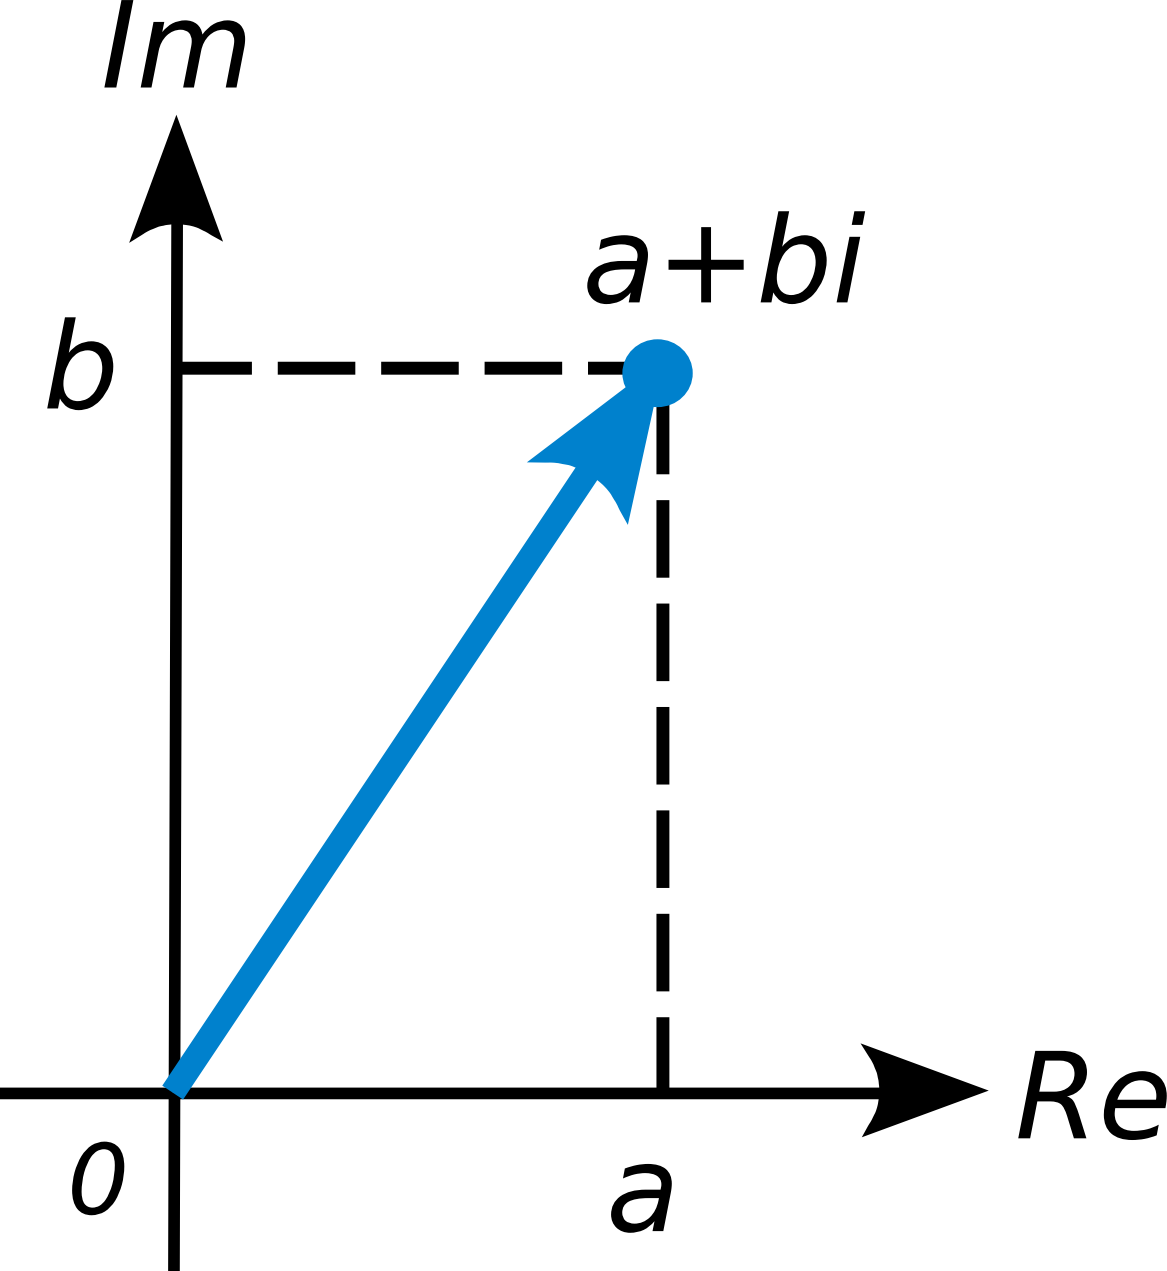
\includegraphics[width=0.8\linewidth,keepaspectratio]{ComplexNumber}
\end{center}
\end{minipage}
}

%
%  \begin{columns}
%    \begin{column}{0.6\linewidth}
%      \raggedleft
%      A complex number $\mathbf{z}$ has the form $\mathbf{z} = z_1 + z_2i$, where \\
%      $z_1$ and $z_2$ are real numbers; \\
%      $z_1$ is called the real part \\
%      and $z_2$ the imaginary part.
%    \end{column}
%    \begin{column}{0.4\linewidth}
%      \centering
%      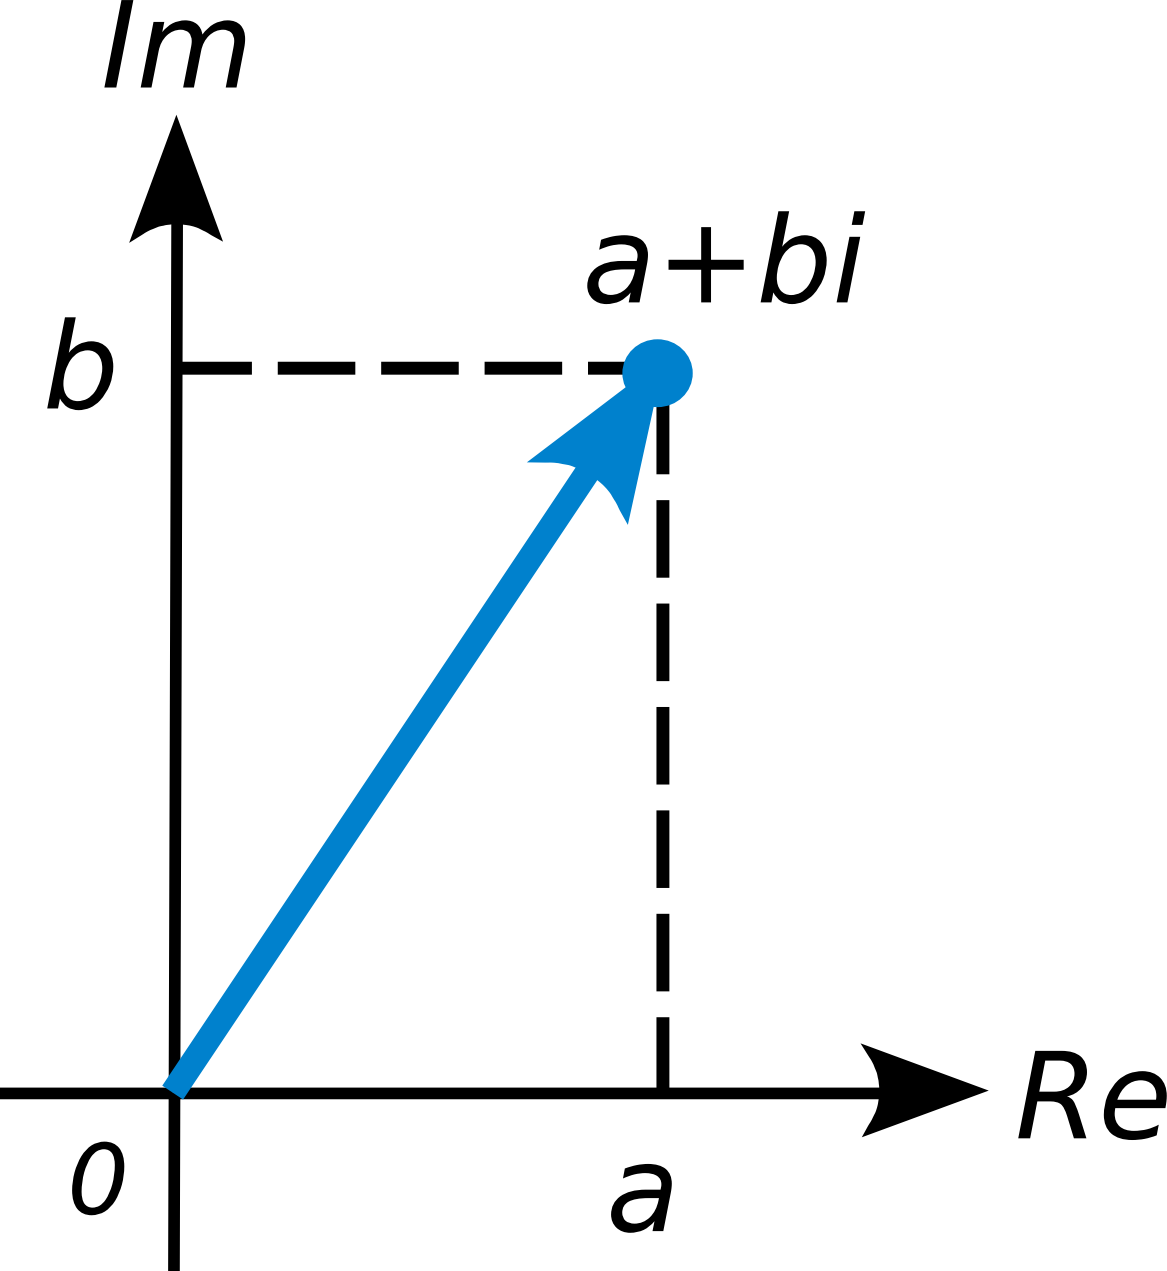
\includegraphics[width=\linewidth]{ComplexNumber}
%    \end{column}
%  \end{columns}

  The set of complex numbers is a field with the two operations:
  \begin{itemize}
  \item
    \emph{addition:} if $\mathbf{z} = \mathbf{x} + \mathbf{y}$, where $\mathbf{x} = x_1 + x_2i$ and $\mathbf{y} = y_1 + y_2i$
    then: $z_1 = x_1 + y_1$, and $z_2 = x_2 + y_2$.

  \item
    \emph{multiplication:} if $\mathbf{z} = \mathbf{x} \cdot
    \mathbf{y}$, then:
 $z_1 = x_1\cdot y_1 - x_2 \cdot y_2$, and $z_2 = x_2\cdot y_1 + x_1\cdot y_2$.
  \end{itemize}
\end{frame}

%%%%%%%%%%%%%%%%%%%%%%%%%%%%%%%%%%%%%%%%%%%%%%%%%%%%%%%%%%%%%%%%%%%%%%%%%%%%%%%%%%%
\begin{frame}[fragile]\frametitle{Naive complex numbers in Python}
 Python object that implements a complex number.
\begin{lstlisting}[showstringspaces=false]
class ComplexNum(object):
  "A complex number z = z1 + z2*i."
  def __init__(self, z1, z2):
    self.re = z1
    self.im = z2
  def __add__(self, other):
    return ComplexNum(
      self.re+other.re, self.im+other.im)
  def __mul__(self, other):
    return ComplexNum(
      self.re*other.re - self.im*other.im,
      self.re*other.im + self.im*other.re)
  def __str__(self):
    return ("%g + %gi" % (self.re, self.im))
  def __eq__(self, other):
    return (self.re == other.re) \
           and (self.im == other.im)
\end{lstlisting}

\end{frame}

%%%%%%%%%%%%%%%%%%%%%%%%%%%%%%%%%%%%%%%%%%%%%%%%%%%%%%%%%%%%%%%%%%%%%%%%%%%%%%%%%%%
\begin{frame}[fragile]\frametitle{What does \texttt{ComplexNum} do?}
  \begin{columns}
    \begin{column}[t]{0.5\linewidth}
      We can create complex numbers by initializing them with the real
      and imaginary part:
\begin{lstlisting}
>>> u = ComplexNum(1,0)
>>> i = ComplexNum(0,1)
>>> z = ComplexNum(1,1)
\end{lstlisting}
    \end{column}
    \begin{column}[t]{0.5\linewidth}
      The str method provides the familiar
      representation:
\begin{lstlisting}
>>> print(u)
1 + 0i
>>> print(i)
0 + 1i
>>> print(z)
1 + 1i
\end{lstlisting}
    \end{column}
  \end{columns}

  %\+
  \begin{columns}
    \begin{column}[t]{0.5\linewidth}
      The add method makes the ``\texttt{+}'' operator work:
\begin{lstlisting}
>>> w = u + i
>>> print(w)
1 + 1i
\end{lstlisting}
    \end{column}
    \begin{column}[t]{0.5\linewidth}
      The mul method makes the ``\texttt{*}'' operator work:
\begin{lstlisting}
>>> m = i*i
>>> print(m)
-1 + 0i
\end{lstlisting}
    \end{column}
  \end{columns}
\end{frame}

%%%%%%%%%%%%%%%%%%%%%%%%%%%%%%%%%%%%%%%%%%%%%%%%%%%%%%%%%%%%%%%%%%%%%%%%%%%%%%%%%%%
\begin{frame}[fragile]\frametitle{Exercises}
\begin{itemize}
\item Add a to\_power method to class \texttt{ComplexNum},
    that takes an integer number as argument and returns the complex
    number raised to that power.

\item 
    Example:
\begin{lstlisting}
>>> z = Complex(1,1)
>>> w = z.to_power(3)
>>> print(w)
-2 + i2
\end{lstlisting}

\item 
Verify that z.to\_power(1),
    z.to\_power(2) and z.to\_power(3) yield the
    same result as z, z*z and
    z*z*z.
\end{itemize}
\end{frame}



%%%%%%%%%%%%%%%%%%%%%%%%%%%%%%%%%%%%%%%%%%%%%%%%%%%%%%%%%%%%%%%%%%%%%%%%%%%%%%%%%%%
\begin{frame}[fragile]\frametitle{Exercises}
%%%%  \begin{exercise}
    Modify the mul method of class \texttt{ComplexNum}:
    \begin{itemize}
    \item If second argument \texttt{other} is an object of class
      \texttt{int} (integer) or \texttt{float} (floating-point
      number) then return the result of scalar multiplication by that number.
    \item If second argument \texttt{other} is an object of class
      \texttt{ComplexNum}, then return the result of complex
      multiplication by that number.
    \end{itemize}
%%%%  \end{exercise}
\end{frame}

%%%%%%%%%%%%%%%%%%%%%%%%%%%%%%%%%%%%%%%%%%%%%%%%%%%%%%%%%%%%%%%%%%%%%%%%%%%%%%%%%%%
\begin{frame}[fragile]\frametitle{\texttt{Vector} vs \texttt{ComplexNum}}

  There's a lot of similarities in the two classes!

  How can we share code between the two?

  \begin{columns}[t]
    \begin{column}{0.5\linewidth}
\begin{lstlisting}[basicstyle=\tiny\ttfamily,showstringspaces=false]
class Vector(object):
  def __init__(self, x, y):
    self.x = x
    self.y = y
  def __eq__(self, other):
    return (self.x == other.x) \
            and (self.y == other.y)
  def __add__(self, other):
    return Vector(
      self.x+other.x, self.y+other.y)
  def __mul__(self, scalar):
    return Vector(
      scalar*self.x,
      scalar*self.y)
  def __str__(self):
    return ("<%g,%g>" % (self.x, self.y))
\end{lstlisting}
    \end{column}
    
    \begin{column}{0.5\linewidth}
\begin{lstlisting}[basicstyle=\tiny\ttfamily,showstringspaces=false]
class ComplexNum(object):
  def __init__(self, z1, z2):
     self.re = z1
     self.im = z2
  def __eq__(self, other):
      return (self.re == other.re) \
           and (self.im == other.im)
  def __add__(self, other):
      return ComplexNum(
      self.re+other.re, self.im+other.im)
  def __mul__(self, other):
    return ComplexNum(
      self.re*other.re - self.im*other.im,
      self.re*other.im + self.im*other.re)
  def __str__(self):
     return ("%g + %gi" % (self.re, self.im))
\end{lstlisting}
    \end{column}
  \end{columns}
\end{frame}


%%%%%%%%%%%%%%%%%%%%%%%%%%%%%%%%%%%%%%%%%%%%%%%%%%%%%%%%%%%%%%%%%%%%%%%%%%%%%%%%%%%
\begin{frame}[fragile]\frametitle{\emph{Vectors} and \emph{Complex Numbers}}

\adjustbox{valign=t}{
\begin{minipage}{0.45\linewidth}
 Complex Numbers are in $1-1$ correspondence with
      points in the real plane $\mathbb{R}^2$: the set $\mathbb{C}$ of
      Complex Numbers is the set of real \emph{2D} vectors.
\end{minipage}
}
\hfill
\adjustbox{valign=t}{
\begin{minipage}{0.4\linewidth}
\begin{center}
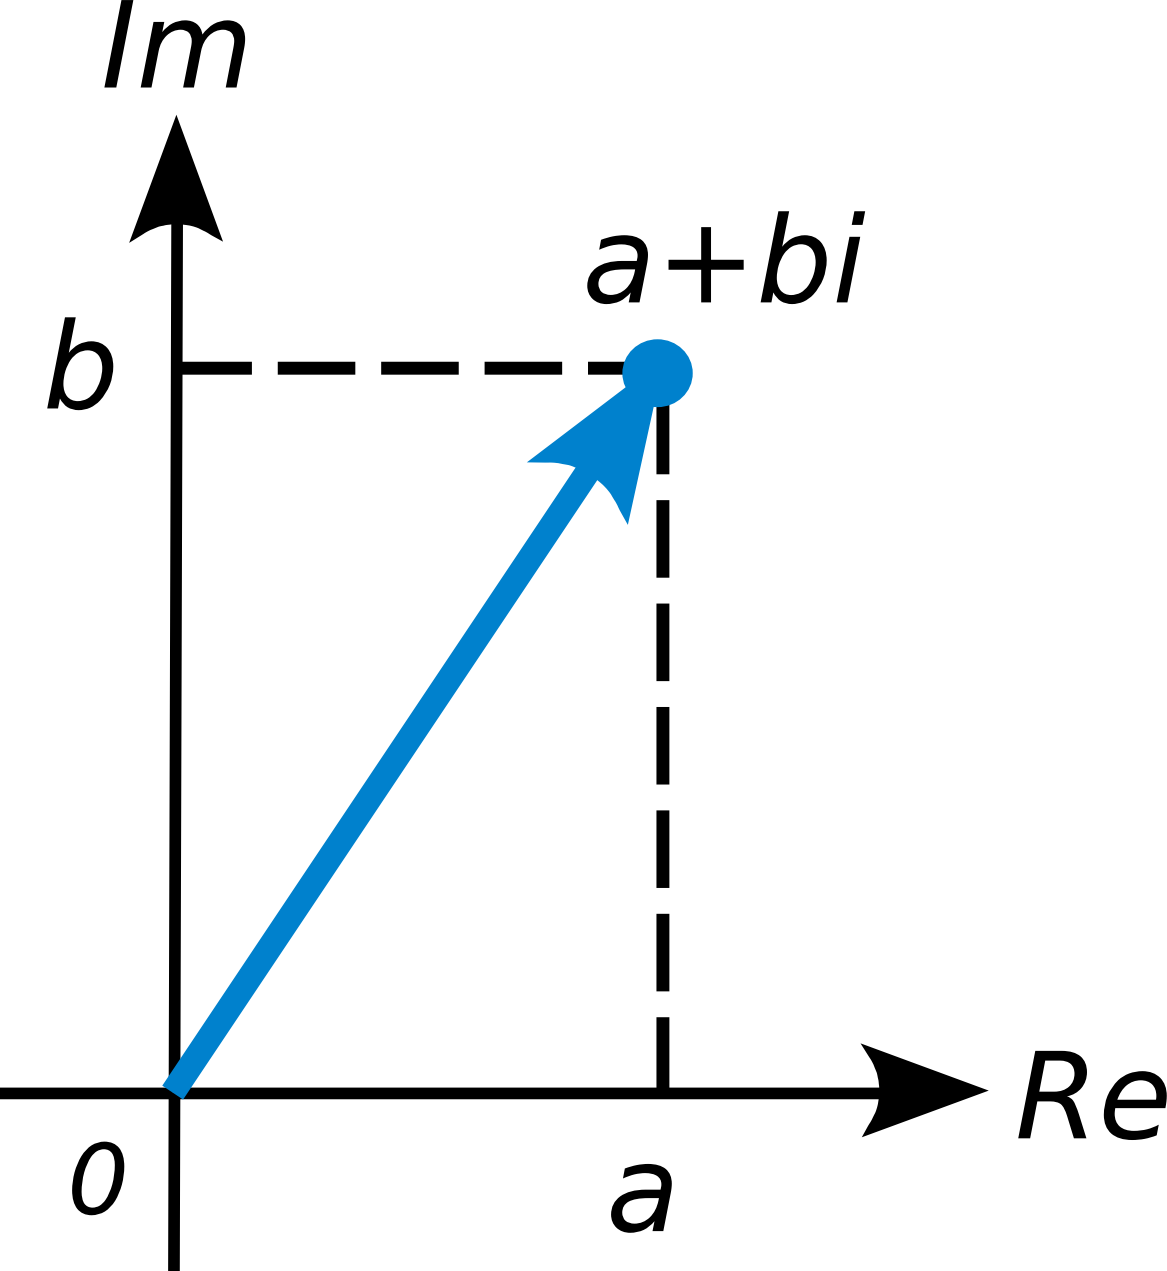
\includegraphics[width=\linewidth,keepaspectratio]{ComplexNumber}
\end{center}
\end{minipage}
}

\begin{itemize}
\item  So we can define the class of Complex Numbers as the class of
  Vectors augmented with a multiplication operation.
\item   So: a Complex Number is a Vector plus some behavior.
\end{itemize}
\end{frame}
%
%%%%%%%%%%%%%%%%%%%%%%%%%%%%%%%%%%%%%%%%%%%%%%%%%%%%%%%%%%%%%%%%%%%%%%%%%%%%%%%%%%%%
%\begin{frame}[fragile]\frametitle{The \texttt{isinstance} function}
%  The \texttt{isinstance($x$, $C$)} function returns \texttt{True} if
%  object $x$ is an instance of class $C$.
%
%  %\+
%  \begin{columns}
%    \begin{column}{0.5\linewidth}
%\begin{lstlisting}
%>>> isinstance(z, ComplexNum)
%True
%>>> isinstance(z, Vector)
%True
%\end{lstlisting}
%    \end{column}
%    \begin{column}{0.4\linewidth}
%      \raggedleft
%      An instance of \texttt{ComplexNum} is also an instance of
%      \texttt{Vector} by inheritance.
%    \end{column}
%  \end{columns}
%\end{frame}
%
%%%%%%%%%%%%%%%%%%%%%%%%%%%%%%%%%%%%%%%%%%%%%%%%%%%%%%%%%%%%%%%%%%%%%%%%%%%%%%%%%%%%
%\begin{frame}[fragile]\frametitle{The \texttt{isinstance} function}
%  The \texttt{isinstance($x$, $C$)} function returns \texttt{True} if
%  object $x$ is an instance of class $C$.
%
%  %\+
%  \begin{columns}
%    \begin{column}{0.5\linewidth}
%\begin{lstlisting}
%>>> isinstance(v, Vector)
%True
%>>> isinstance(v, ComplexNum)
%False
%\end{lstlisting}
%    \end{column}
%    \begin{column}{0.5\linewidth}
%      \raggedleft
%      \emph{However,} instances of \texttt{Vector} are \emph{not}
%      instances of \texttt{ComplexNum}.
%    \end{column}
%  \end{columns}
%\end{frame}
%
%%%%%%%%%%%%%%%%%%%%%%%%%%%%%%%%%%%%%%%%%%%%%%%%%%%%%%%%%%%%%%%%%%%%%%%%%%%%%%%%%%%%
%\begin{frame}[fragile]\frametitle{The \texttt{isinstance} function}
%  The \texttt{isinstance($x$, $C$)} function returns \texttt{True} if
%  object $x$ is an instance of class $C$.
%
%  %\+
%  \begin{columns}
%    \begin{column}{0.5\linewidth}
%\begin{lstlisting}
%>>> isinstance(1, int)
%True
%>>> isinstance(0.5, float)
%True
%>>> isinstance("hi!", str)
%True
%\end{lstlisting}
%    \end{column}
%    \begin{column}{0.5\linewidth}
%      \raggedleft
%      Basic Python objects are instances of built-in classes.
%    \end{column}
%  \end{columns}
%\end{frame}

%%%%%%%%%%%%%%%%%%%%%%%%%%%%%%%%%%%%%%%%%%%%%%%%%%%%%%%%%%%%%%%%%%%%%%%%%%%%%%%%%%%
\begin{frame}[fragile]\frametitle{Inheritance, I}

  \begin{columns}[t]
    \begin{column}{0.5\linewidth}
\begin{lstlisting}[basicstyle=\tiny\ttfamily,showstringspaces=false]
class Vector(object):

  def __init__(self, x, y):
    self.x = x
    self.y = y

  def __eq__(self, other):
    return (self.x == other.x) \
            and (self.y == other.y)

  def __add__(self, other):
    return self.__class__(
      self.x+other.x, self.y+other.y)

  def __mul__(self, scalar):
    return Vector(
      scalar*self.x,
      scalar*self.y)

  def __str__(self):
    return ("<%g,%g>" % (self.x, self.y))
\end{lstlisting}
    \end{column}
    \begin{column}{0.5\linewidth}
\begin{lstlisting}[basicstyle=\tiny\ttfamily,showstringspaces=false]
class ComplexNum(Vector):

  def __mul__(self, other):
    return ComplexNum(
      self.x*other.x - self.y*other.y,
      self.x*other.y + self.y*other.x)

  def __str__(self):
    return ("%g + %gi" % (self.x, self.y))
\end{lstlisting}

\begin{itemize}
\item  \texttt{class ComplexNum} is a
      \emph{child}/\emph{descendant}/\emph{subclass} of class \texttt{Vector}.

\item 
       \texttt{class Vector} is a
      \emph{parent}/\emph{ancestor}/\emph{superclass} of class
      \texttt{ComplexNum}.
\end{itemize}

    \end{column}
  \end{columns}

\end{frame}

%%%%%%%%%%%%%%%%%%%%%%%%%%%%%%%%%%%%%%%%%%%%%%%%%%%%%%%%%%%%%%%%%%%%%%%%%%%%%%%%%%%
\begin{frame}[fragile]\frametitle{Inheritance, II}

  \begin{columns}[t]
    \begin{column}{0.5\linewidth}
\begin{lstlisting}[basicstyle=\tiny\ttfamily,showstringspaces=false]
class Vector(object):

  def __init__(self, x, y):
    self.x = x
    self.y = y

  def __eq__}(self, other):
    return (self.x == other.x) \
            and (self.y == other.y)

  def __add__(self, other):
    return self.__class__(
      self.x+other.x, self.y+other.y)

  def __mul__(self, scalar):
    return Vector(
      scalar*self.x,
      scalar*self.y)

  def __str__(self):
    return ("<%g,%g>" % (self.x, self.y))
\end{lstlisting}
    \end{column}
    \begin{column}{0.5\linewidth}
\begin{lstlisting}[basicstyle=\tiny\ttfamily,showstringspaces=false]
class ComplexNum(Vector):

  def __mul__(self, other):
    return ComplexNum(
      self.x*other.x - self.y*other.y,
      self.x*other.y + self.y*other.x)

  def __str__(self):
    return ("%g + %gi" % (self.x, self.y))
\end{lstlisting}

      %\+
  All methods defined in class \texttt{Vector} are automatically
  defined \emph{(inherited)} in class \texttt{ComplexNum}.
    \end{column}
  \end{columns}
\end{frame}

%%%%%%%%%%%%%%%%%%%%%%%%%%%%%%%%%%%%%%%%%%%%%%%%%%%%%%%%%%%%%%%%%%%%%%%%%%%%%%%%%%%
\begin{frame}[fragile]\frametitle{Inheritance, III}

  \begin{columns}[t]
    \begin{column}{0.5\linewidth}
\begin{lstlisting}[basicstyle=\tiny\ttfamily,showstringspaces=false]
class Vector(object):

  def __init__(self, x, y):
    self.x = x
    self.y = y

  def __eq__(self, other):
    return (self.x == other.x) \
            and (self.y == other.y)

  def __add__(self, other):
    return self.__class__(
      self.x+other.x, self.y+other.y)

  def __mul__(self, other):
    return Vector(
      scalar*self.x,
      scalar*self.y)

  def __str__}(self):
    return ("<%g,%g>" % (self.x, self.y))
\end{lstlisting}
    \end{column}
    \begin{column}{0.5\linewidth}
\begin{lstlisting}[basicstyle=\tiny\ttfamily,showstringspaces=false]
class ComplexNum(Vector):

  def __mul__(self, other):
    return ComplexNum(
      self.x*other.x - self.y*other.y,
      self.x*other.y + self.y*other.x)

  def __str__(self):
    return ("%g + %gi" % (self.x, self.y))
\end{lstlisting}

      \small
      %\+
      Methods mul and str are
      defined in both classes: instances of a class use the
      definition from that class.

      %\+
      We say that \texttt{ComplexNum} \emph{overrides} those
      methods from \texttt{Vector}.
    \end{column}
  \end{columns}
\end{frame}

%%%%%%%%%%%%%%%%%%%%%%%%%%%%%%%%%%%%%%%%%%%%%%%%%%%%%%%%%%%%%%%%%%%%%%%%%%%%%%%%%%%%
%\begin{frame}[fragile]\frametitle{}
%  What happens if a descendant class re-defines a init
%  method?
%
%
%  %\+ 
% {\em
%    The init in the descendant class
%    \emph{overrides} the method in the ancestor class.  So
%    init of the parent class(es) will not be called.
%    }
%\end{frame}



%%%%%%%%%%%%%%%%%%%%%%%%%%%%%%%%%%%%%%%%%%%%%%%%%%%%%%%%%%%%%%%%%%%%%%%%%%%%%%%%%%%
\begin{frame}[fragile]\frametitle{Method chaining}

  Actually, init is not special in this regard.

  %\+ 
  When any instance method is called, Python only calls the first
  constructor it can find in the
  \href{http://www.python.org/download/releases/2.3/mro/}{class
    inheritance call-chain}.

  %\+ 
  \textbf{You can always call a superclass method by prefixing it
    with the superclass name and explicitly writing ``\texttt{self}''
    as the first argument:}
    \begin{lstlisting}
class ComplexNum(Vector):
  # ...
  def print_as_vector(self):
    return Vector.__str__(self)
    \end{lstlisting}
\end{frame}

%%%%%%%%%%%%%%%%%%%%%%%%%%%%%%%%%%%%%%%%%%%%%%%%%%%%%%%%%%%%%%%%%%%%%%%%%%%%%%%%%%%
\begin{frame}[fragile]\frametitle{Inheritance, IV}
Take a look at this Python interaction:
\begin{lstlisting}
>>> z = ComplexNum(1,0)
>>> print(z)
1 + i0
>>> w = ComplexNum(0,1)
>>> print(w)
0 + i1
>>> u = z + w
>>> print(u)
\end{lstlisting}

%\only<1>{\em  What do you think will be printed now?}
%\only<2>{%
%  \vspace{-1.5em}
%\begin{semiverbatim}
%\HL{<1,1>}
%\end{semiverbatim}
 This is no \texttt{ComplexNum}! What's happening here?

\end{frame}

%%%%%%%%%%%%%%%%%%%%%%%%%%%%%%%%%%%%%%%%%%%%%%%%%%%%%%%%%%%%%%%%%%%%%%%%%%%%%%%%%%%
\begin{frame}[fragile]\frametitle{Inheritance, V}
  The answer is in the code:
    \begin{lstlisting}
class Vector(object):
  # ...
  def __add__(self, other):
    return Vector(self.x+other.x, self.y+other.y)
    \end{lstlisting}
    
    The add method returns a new
    Vector instance, even when called from a
    ComplexNum !
\end{frame}

%%%%%%%%%%%%%%%%%%%%%%%%%%%%%%%%%%%%%%%%%%%%%%%%%%%%%%%%%%%%%%%%%%%%%%%%%%%%%%%%%%%
\begin{frame}[fragile]\frametitle{Inheritance, VI}
  Correct code:
    \begin{lstlisting}
class Vector(object):
  # ...
  def __add__(self, other):
    return self.__class__(self.x+other.x, self.y+other.y)
    \end{lstlisting}
    Use the class of the actual instance that's passed,
    instead of hard-coding a class name.
\end{frame}

%%%%%%%%%%%%%%%%%%%%%%%%%%%%%%%%%%%%%%%%%%%%%%%%%%%%%%%%%%%%%%%%%%%%%%%%%%%%%%%%%%%
\begin{frame}[fragile]\frametitle{Polymorphism, I}

  The multiplication operator ``\texttt{*}'' on instances of the
  Vector class works as \emph{scalar multiplication}:
\begin{lstlisting}
>>> v = Vector(1,0)
>>> print (v * 3)
<3,0>
\end{lstlisting}

  %\+
  The same operator ``\texttt{*}'' on instances of the
  ComplexNum class works as \emph{complex multiplication}:
\begin{lstlisting}
>>> z = ComplexNum(1,1)
>>> w = ComplexNum(2,0)
>>> print (z * w)
2 + i2
\end{lstlisting}

  %\+
  \small
  The ability to implement different behavior for the same
  method/operator in different classes is called \emph{polymorphism}.

\end{frame}

%%%%%%%%%%%%%%%%%%%%%%%%%%%%%%%%%%%%%%%%%%%%%%%%%%%%%%%%%%%%%%%%%%%%%%%%%%%%%%%%%%%
\begin{frame}[fragile]\frametitle{Polymorphism, II}

  You may observe that an integer is (in particular) a complex number,
  still we cannot multiply a \texttt{ComplexNum} instance by an
  integer number:
\begin{lstlisting}
>>> print (z * 3)
Traceback (most recent call last):
  File "<stdin>", line 1, in <module>
  File "vector_and_complexnum.py", line 20, in __mul__
    self.x*other.x - self.y*other.y,
AttributeError: 'int' object has no attribute 'x'
\end{lstlisting}

\end{frame}

%%%%%%%%%%%%%%%%%%%%%%%%%%%%%%%%%%%%%%%%%%%%%%%%%%%%%%%%%%%%%%%%%%%%%%%%%%%%%%%%%%%
\begin{frame}[fragile]\frametitle{Polymorphism, III}

\begin{lstlisting}
>>> print (z * 3)
Traceback (most recent call last):
  File "<stdin>", line 1, in <module>
  File "vector_and_complexnum.py", line 20, in __mul__
    self.x*other.x - self.y*other.y,
AttributeError: 'int' object has no attribute 'x'
\end{lstlisting}

  %\+ 
  Our code for mul implicitly assumes
  that argument other has attributes \texttt{x} and
  \texttt{y}, and integers do not!
\end{frame}








%%%%%%%%%%%%%%%%%%%%%%%%%%%%%%%%%%%%%%%%%%%%%%%%%%%%%%%%%%%%%%%%%%%%%%%%%%%%%%%%%%%
\begin{frame}[fragile]\frametitle{Recall: Object Oriented Programming}

\begin{itemize}
\item A Python object is a bundle of variables and functions.
\item Defined  by the object's \emph{class}.
\item  From class, many objects can be \emph{instantiated}.
\item Different instances can assign different values to the object variables.
\end{itemize}
\end{frame}

 
\section[IO]{Module 7: IO}
%%%%%%%%%%%%%%%%%%%%%%%%%%%%%%%%%%%%%%%%%%%%%%%%%%%%%%%%%%%%%%%%%%%%%%%%%%%%%%%%%%
\begin{frame}[fragile]\frametitle{}
\begin{center}
{\Large Input/Output}
\end{center}
\end{frame}


%%%%%%%%%%%%%%%%%%%%%%%%%%%%%%%%%%%%%%%%%%%%%%%%%%%%%%%%%%%%%%%%%%%%%%%%%%%%%%%%%%%
\begin{frame}[fragile]\frametitle{Asking the user for input}
\begin{itemize}
\item  Python provides a built-in function called input that gets input from
the keyboard:
\item When the user presses Return or Enter, the program
resumes and input returns what the user typed as a string.
\begin{lstlisting}
>>> input = input()
Some silly stuff
>>> print(input)
Some silly stuff
\end{lstlisting}
\item Before getting input from the user, it is a good idea to print a prompt telling the
user what to input:
\begin{lstlisting}
>>> speed = input(prompt)
What...is the airspeed velocity of an unladen swallow?
What do you mean, an African or a European swallow?
>>> int(speed)
ValueError: invalid literal for int() with base 10:
\end{lstlisting}
\end{itemize}
\end{frame}

%%%%%%%%%%%%%%%%%%%%%%%%%%%%%%%%%%%%%%%%%%%%%%%%%%%%%%%%%%%%%%%%%%%%%%%%%%%%%%%%%%%
\begin{frame}[fragile]\frametitle{Prompt}
\begin{itemize}
\item  Combine prompt and input
\begin{lstlisting}
>>> prompt = 'What...is the airspeed velocity of an unladen swallow?\n'
>>> speed = input(prompt)
What...is the airspeed velocity of an unladen swallow?
17
>>> int(speed)
17
>>> int(speed) + 5
22
\end{lstlisting}
\item But if the user types something other than a string of digits, you get an error:
\begin{lstlisting}
>>> name = input('What is your name?\n')
What is your name?
Chuck
>>> print(name)
Chuck
\end{lstlisting}
\end{itemize}
\end{frame}

%%%%%%%%%%%%%%%%%%%%%%%%%%%%%%%%%%%%%%%%%%%%%%%%%%%%%%%%%%%%%%%%%%%%%%%%%%%%%%%%%%%
\begin{frame}[fragile]\frametitle{File IO}
\begin{itemize}
\item Can read data from a file, or write into a file
\item The open function takes two arguments, the name of the file, and the mode. The modes are:
\begin{lstlisting}
    'r': open a file for reading
    'w': open a file for writing. Caution: this will overwrite any previously existing file
    'a': append. Write to the end of a file.
\end{lstlisting}
\item The function returns a file object that performs the various tasks you'll be performing: a\_file = open(filename, mode). 
\begin{lstlisting}
    file.read(): read the entire contents of a file into a string
    file.write(some_string): writes to the file, note this doesn't automatically include any new lines.
    file.flush(): write out any buffered writes
    file.close(): close the open file. 
\end{lstlisting}
\end{itemize}
\end{frame}

%%%%%%%%%%%%%%%%%%%%%%%%%%%%%%%%%%%%%%%%%%%%%%%%%%%%%%%%%%%%%%%%%%%%%%%%%%%%%%%%%%%
\begin{frame}[fragile]\frametitle{Writing a file to disk}
\begin{lstlisting}
# Create the file temp.txt, and get it ready for writing
f = open("temp.txt", "w")
f.write("This is my first file! The end!\n")
f.write("Oh wait, I wanted to say something else.")
f.close()

# Create a file numbers.txt and write the numbers from 0 to 24 there
f = open("numbers.txt", "w")
for num in range(25):
    f.write(str(num)+'\n')
f.close()
\end{lstlisting}
\end{frame}


%%%%%%%%%%%%%%%%%%%%%%%%%%%%%%%%%%%%%%%%%%%%%%%%%%%%%%%%%%%%%%%%%%%%%%%%%%%%%%%%%%%
\begin{frame}[fragile]\frametitle{Reading a file from disk}
\begin{lstlisting}
# We now open the file for reading
f2 = open("temp.txt", "r")
# And we read the full content of the file in memory, as a big string
f2_content = f2.read()
f2.close()

# Read the file in the cell above, the content is in f2_content

# Split the content of the file using the newline character \n
lines = f2_content.split("\n")

# Iterate through the line variable (it is a list of strings)
# and then print the length of each line
for line in lines:
    print("Length of line `{0}` is {1}".format(line,len(line)))
\end{lstlisting}
\end{frame}

%%%%%%%%%%%%%%%%%%%%%%%%%%%%%%%%%%%%%%%%%%%%%%%%%%%%%%%%%%%%%%%%%%%%%%%%%%%%%%%%%%%
\begin{frame}[fragile]\frametitle{Reading a file from disk}
\begin{lstlisting}
# We now open the file for reading
f2 = open("numbers.txt", "r")
# And we read the full content of the file in memory, as a big string
f2_content = f2.read()
f2.close()

lines = f2_content.split("\n")
print(lines)

numbers = [int(line) for line in lines if len(line)>0]
print(numbers)
\end{lstlisting}
\end{frame}

%%%%%%%%%%%%%%%%%%%%%%%%%%%%%%%%%%%%%%%%%%%%%%%%%%%%%%%%%%%%%%%%%%%%%%%%%%%%%%%%%%%
\begin{frame}[fragile]\frametitle{Using try, except, and open}
\begin{lstlisting}
fname = input('Enter the file name: ')
try:
	fhand = open(fname)
except:
	print('File cannot be opened:', fname)
	exit()
count = 0
for line in fhand:
	if line.startswith('Subject:'):
		count = count + 1
print('There were', count, 'subject lines in', fname)
\end{lstlisting}
\end{frame}

%%%%%%%%%%%%%%%%%%%%%%%%%%%%%%%%%%%%%%%%%%%%%%%%%%%%%%%%%%%%%%%%%%%%%%%%%%%%%%%%%%%
\begin{frame}[fragile]\frametitle{Searching through a file}
\begin{lstlisting}
fhand = open('mbox-short.txt')
count = 0
for line in fhand:
	line = line.rstrip()
	if line.startswith('From:'):
		print(line)
\end{lstlisting}
\end{frame}
%
%
%%%%%%%%%%%%%%%%%%%%%%%%%%%%%%%%%%%%%%%%%%%%%%%%%%%%%%%%%%%%%%%%%%%%%%%%%%%%%%%%%%%%
%\begin{frame}[fragile]\frametitle{File I/O, I}
%
%%  \begin{describe}
%  {\ttfamily stream = open(path,mode)}
%    Return a Python \texttt{file} object for reading or writing the
%    file located at \texttt{path}.  Mode is one of '\texttt{r}',
%    '\texttt{w}' or '\texttt{a}' for reading, writing (truncates on open), appending.
%    You can add a `\texttt{+}' character to enable read+write (other
%    effects being the same).
%%  \end{describe}
%
%%  \begin{describe}
%  {\ttfamily \emph{stream}.close()}
%    Close an open file.
%%  \end{describe}
%
%%  \begin{describe}
%  {\ttfamily \textbf{for} line \textbf{in} stream:}
%    Loop over lines in the file one by one.
%%  \end{describe}
%
%%  \begin{references}
%%    \url{http://docs.python.org/library/stdtypes.html#file-objects}
%%  \end{references}
%\end{frame}
%
%%%%%%%%%%%%%%%%%%%%%%%%%%%%%%%%%%%%%%%%%%%%%%%%%%%%%%%%%%%%%%%%%%%%%%%%%%%%%%%%%%%%
%\begin{frame}[fragile]\frametitle{File I/O, II}
%
%  The \lstinline|read(n)| method can be used to read \emph{at most}
%  \lstinline|n| bytes from a file-like object:
%\begin{lstlisting}
%>>> s = stream.read(2)
%>>> print(s)
%'py'
%\end{lstlisting}
%  If \lstinline|n| is omitted, \texttt{read()} reads until end-of-file.
%
%%  \begin{references}
%%    \url{http://docs.python.org/library/stdtypes.html#file-objects}
%%  \end{references}
%\end{frame}


%%%%%%%%%%%%%%%%%%%%%%%%%%%%%%%%%%%%%%%%%%%%%%%%%%%%%%%%%%%%%%%%%%%%%%%%%%%%%%%%%%%
\begin{frame}[fragile]\frametitle{Filesystem operations, I}
\texttt{os} module functions:

  \begin{lstlisting}
  os.getcwd(),   os.chdir(path)
  \end{lstlisting}
   Get current working directory. Change to \texttt{path}.
  \begin{lstlisting}
  os.listdir(dir)
  \end{lstlisting}
    Return list of entries in directory \texttt{dir} (omitting
    `\texttt{.}' and `\texttt{..}')
  \begin{lstlisting}
  os.mkdir(path)
  \end{lstlisting}
    Create a directory; fails if the directory already exists.
    Assumes that all parent directories exist already.
  \begin{lstlisting}
  os.makedirs(path)
\end{lstlisting}
Create a directory; no-op if the directory already exists.
Creates all the intermediate-level directories needed to contain the leaf.
%\begin{lstlisting}
%  os.rename(old,new)
%\end{lstlisting}
%    Rename a file or directory from \texttt{old} to \texttt{new}.
\end{frame}


%%%%%%%%%%%%%%%%%%%%%%%%%%%%%%%%%%%%%%%%%%%%%%%%%%%%%%%%%%%%%%%%%%%%%%%%%%%%%%%%%%%
\begin{frame}[fragile]\frametitle{Filesystem operations, II}
  These functions are available from the \texttt{os.path} module.

\begin{lstlisting}
os.path.exists(path), os.path.isdir(path), os.path.isfile(path)
\end{lstlisting}
    Return \texttt{True} if \texttt{path} exists / is a directory / is
    a regular file.
  \begin{lstlisting}
os.path.basename(path),
os.path.dirname(path)
  \end{lstlisting}
    Return the base name (the part after the last `\texttt{/}'
    character) or the directory name (the part before the last
    \texttt{/} character).
  \begin{lstlisting}
  os.path.abspath(path)
  \end{lstlisting}
    Make \texttt{path} absolute (i.e., start with a \texttt{/}).
\end{frame}

%%%%%%%%%%%%%%%%%%%%%%%%%%%%%%%%%%%%%%%%%%%%%%%%%%%%%%%%%%%%%%%%%%%%%%%%%%%%%%%%%%%%
%\begin{frame}[fragile]\frametitle{Exercises}
%Write a function \lstinline|cat(filename)| that prints the whole contents of a file. Test it with the https://raw.github.com/gc3-uzh-ch/python-course/master/welcome.py file:
%\begin{lstlisting}
%>>> cat('welcome.py')
%#! /usr/bin/env python
%
%print ("Welcome to Python!")
%\end{lstlisting}
%Write a function \lstinline|load_data(filename)| that reads a file containing one integer number per line, and return a list of the integer values. Test it with the https://raw.github.com/gc3-uzh-ch/python-course/master/values.dat  file:
%\begin{lstlisting}
%>>> load_data('values.dat')
%[299850, 299740, 299900, 300070, 299930]
%\end{lstlisting}
%\end{frame}

%%%%%%%%%%%%%%%%%%%%%%%%%%%%%%%%%%%%%%%%%%%%%%%%%%%%%%%%%%%%%%%%%%%%%%%%%%%%%%%%%%%
\begin{frame}[fragile]\frametitle{Exercises}
 \begin{itemize}
    \item Write a program that reads the https://raw.github.com/gc3-uzh-ch/python-course/master/euro.csv
    file and populates a dictionary from it: currency names (first column) are the dictionary keys, conversion rates (second column) are the dictionary values.
%    \item Write a function that reads a file and returns its content as a list of strings (one string per line). Read the file with filename data/restaurant-names.txt. If you stored your notebook under Student\_Notebooks the full filename is /data/restaurant-names.txt
\end{itemize}

\end{frame}

%%%%%%%%%%%%%%%%%%%%%%%%%%%%%%%%%%%%%%%%%%%%%%%%%%%%%%%%%%%%%%%%%%%%%%%%%%%%%%%%%%%
\begin{frame}[fragile]\frametitle{Exercises}
 \begin{itemize}
    \item Write a function that reads the n-th column of a CSV file and returns its contents. (Reuse the function that you wrote above.) Then reads the file data/baseball.csv and return the content of the 5th column (team).
    \item The command below will create a file called phonetest.txt. Write code that:
    Reads the file phonetest.txt;
    Write a function that takes as input a string, and removes any non-digit characters;
    Print out the "clean" string, without any non-digit characters;
\end{itemize}
\end{frame}

%%%%%%%%%%%%%%%%%%%%%%%%%%%%%%%%%%%%%%%%%%%%%%%%%%%%%%%%%%%%%%%%%%%%%%%%%%%%%%%%%%%
\begin{frame}[fragile]\frametitle{Exercises}
\begin{itemize}
\item
    Write a function \lstinline|wordcount(filename)| that reads a text file and returns a dictionary, mapping words into occurrences (disregarding case) of that word in the text.  
    Test it with the https://raw.github.com/gc3-uzh-ch/python-course/master/lorem\_ipsum.txt file:
    \begin{lstlisting}
>>> wordcount('lorem_ipsum.txt')
{'and': 3, 'model': 1, 'more-or-less': 1,
 'letters': 1, ...
    \end{lstlisting}
%\item
%     For the purposes of this exercise, a ``word'' is defined as a sequence of letters and the character ``-'', i.e., ``e-mail'' and ``more-or-less'' should both be counted as a single word.
%\item
%     You might want to have a look at the http://docs.python.org/2/library/string.html module, for pre-defined sets of alphabetic and punctuation characters.
 \end{itemize}
\end{frame}



%%%%%%%%%%%%%%%%%%%%%%%%%%%%%%%%%%%%%%%%%%%%%%%%%%%%%%%%%%%%%%%%%%%%%%%%%%%%%%%%%%%
\begin{frame}[fragile]\frametitle{Files Operations (recap)}
  \begin{itemize}
  \item input \lstinline{input = open('data', 'r')}
  \item read all \lstinline{S = input.read()}
  \item read N bytes \lstinline{S = input.read(N)}
  \item read next \lstinline{S = input.readline()}
  \item read in lists \lstinline{L = input.readlines()}
  \item output \lstinline{output = open('/tmp/spam', 'w')}
  \item write \lstinline{output.write(S)}
  \item write \lstinline{strings output.writelines(L)}
  \item close \lstinline{output.close()}
  \end{itemize}
\end{frame}

%
%%%%%%%%%%%%%%%%%%%%%%%%%%%%%%%%%%%%%%%%%%%%%%%%%%%%%%%%%%%%%%%%%%%%%%%%%%%%%%%%%%%%
%\begin{frame}[fragile]\frametitle{Command line arguments}
%  The \texttt{sys} module provides access to some variables used or
%  maintained by the interpreter.
%
%  One of such variables is a list containing the arguments passed on
%  the command line.
%
%  
%  \textbf{Example:} This is a simple script that
%  prints the command line arguments used to invoke it:
%
%  \begin{lstlisting}
%import sys
%print(sys.argv)
%  \end{lstlisting}
%
%
%Calling the script as:
%\begin{lstlisting}
%$ python script.py foo bar
%\end{lstlisting}
%yields the following result:
%\begin{lstlisting}
%['script.py', 'foo', 'bar']
%\end{lstlisting}
%\end{frame}
%
%
%%%%%%%%%%%%%%%%%%%%%%%%%%%%%%%%%%%%%%%%%%%%%%%%%%%%%%%%%%%%%%%%%%%%%%%%%%%%%%%%%%%%
%\begin{frame}[fragile]  \frametitle{(Homework)}
%\begin{itemize}
%\item
%    Write a Python program \texttt{rename.py} with the following
%    command-line:
%\begin{lstlisting}[language=sh]
%python rename.py EXT1 EXT2 DIR [DIR ...]
%\end{lstlisting}
%\item
%   \begin{itemize}
%    \item {\bf ext1,ext2} Are file name extensions (without the leading dot), e.g., \texttt{jpg} and \texttt{jpeg}.
%    \item {\bf dir} Is a directory path; possibly, many directories names can
%      be given on the command-line.
%    \end{itemize}
%\item
%    The \texttt{rename.py} command should rename all files in
%    directory DIR, that end with extension \texttt{ext1} to end with
%    extension \texttt{ext2} instead.
%\end{itemize}
%\end{frame}
 
\section[LibI]{Module 8: Libraries I}
%%%%%%%%%%%%%%%%%%%%%%%%%%%%%%%%%%%%%%%%%%%%%%%%%%%%%%%%%%%%%%%%%%%%%%%%%%%%%%%%%%
\begin{frame}[fragile]\frametitle{}
\begin{center}
{\Large Packages: Scientific}
\end{center}
\end{frame}

%%%%%%%%%%%%%%%%%%%%%%%%%%%%%%%%%%%%%%%%%%%%%%%%%%%%%%%%%%%%%%%%%%%%%%%%%%%%%%%%%%%
\begin{frame}[fragile]\frametitle{NumPy: linear algebra package}

\begin{itemize}
\item     \href{http://www.numpy.org/}{NumPy} is a package for linear algebra
  and advanced mathematics in Python.

\item    
  It provides a \emph{fast} implementation of multidimensional
  numerical arrays (C/FORTRAN like), vectors, matrices, tensors and
  operations on them.

\item    
  \emph{Use it if:} you long for MATLAB core features.

  \item Reference: {\footnotesize\url{http://www.numpy.org/}}
  \item Examples: {\footnotesize\url{http://wiki.scipy.org/Numpy_Example_List}}
  \end{itemize}
\end{frame}

%%%%%%%%%%%%%%%%%%%%%%%%%%%%%%%%%%%%%%%%%%%%%%%%%%%%%%%%%%%%%%%%%%%%%%%%%%%%%%%%%%%
\begin{frame}[fragile]\frametitle{NumPy vs. Matlab vs. Bytecode}

    Comparison of $\nabla^2 u = 0$ solvers ($500\times500$, 100 iterations):
    
    \begin{columns}
        \column{0.4\linewidth}
        \begin{table}
            \begin{tabular}{|c|c|}
                \hline
                Platform & Time (s) \\
                \hline \hline
                Python & $\sim$1500.0 \\
                \hline
                NumPy & 29.3 \\
                \hline
                Matlab & $\sim$29.0 \\
                \hline
                Octave & $\sim$60.0 \\
                \hline
                Blitz (C++) & 9.5 \\
                \hline
                Fortran & 2.5 \\
                \hline
                C & 2.2 \\
                \hline
            \end{tabular}
        \end{table}
        \column{0.6\linewidth}
        \begin{center}
            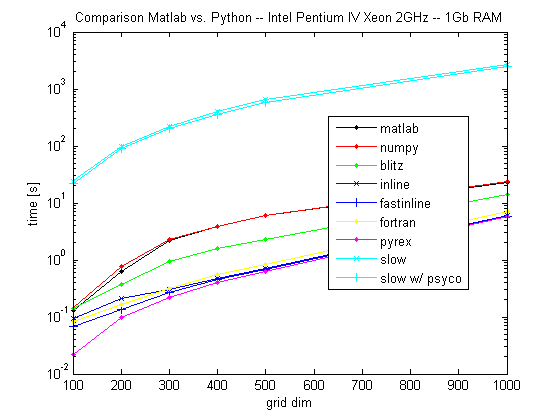
\includegraphics[width=\linewidth]{numpy_perf1.png}
        \end{center}
    \end{columns}

%    (Probably using MKL)
%
%    {\tiny \href{http://www.scipy.org/PerformancePython}{http://www.scipy.org/PerformancePython}}\\
%    {\tiny \href{http://lbolla.info/blog/2007/04/11/numerical-computing-matlab-vs-pythonnumpyweave/}{http://lbolla.info/blog/2007/04/11/numerical-computing-matlab-vs-pythonnumpyweave/}}
\end{frame}

%%%%%%%%%%%%%%%%%%%%%%%%%%%%%%%%%%%%%%%%%%%%%%%%%%%%%%%%%%%%%%%%%%%%%%%%%%%%%%%%%%%
\begin{frame}[fragile]\frametitle{NumPy Array Generation}

    Convert a list to a NumPy array:
    \begin{lstlisting}
>>> import numpy as np
>>> list1 = [1, 2, 3, 4, 5]
>>> x = np.array(list1)
>>> x
array([1, 2, 3, 4, 5])
>>> x.dtype
dtype('int64')
    \end{lstlisting}
    NumPy arrays have values and a data type (\textit{dtype}).
\end{frame}

%%%%%%%%%%%%%%%%%%%%%%%%%%%%%%%%%%%%%%%%%%%%%%%%%%%%%%%%%%%%%%%%%%%%%%%%%%%%%%%%%%%
\begin{frame}[fragile]
    \frametitle{NumPy Array Generation}

    \lstinline|arange()| is similar to \lstinline|range()| for lists:
    \begin{lstlisting}
>>> np.arange(5)
array([0, 1, 2, 3, 4])
>>> np.arange(5.)
array([0., 1., 2., 3., 4.])
    \end{lstlisting}
    
    \lstinline|zeros| for pre-allocation:
    \begin{lstlisting}
>>> np.zeros([2, 3])    # Input is a list
array([[ 0., 0., 0.],
       [ 0., 0., 0.]])
    \end{lstlisting}
\end{frame}

%%%%%%%%%%%%%%%%%%%%%%%%%%%%%%%%%%%%%%%%%%%%%%%%%%%%%%%%%%%%%%%%%%%%%%%%%%%%%%%%%%%
\begin{frame}[fragile]
    \frametitle{NumPy Grid Generation}
   
    Suppose you want to construct a numerical grid.\\
    e.g. $x = x_0 + j \Delta x$, \ $\Delta x = (x_1 - x_0) / N$
    \\~\\
    \lstinline|arange()| uses $\Delta x$ and excludes $x_1$:
    \begin{lstlisting}
>>> x = np.arange(3., 6., 0.5)
array([ 3. ,  3.5,  4. ,  4.5,  5. ,  5.5])
    \end{lstlisting}
    \lstinline|linspace()| uses $N+1$ and includes $x_1$:
    \begin{lstlisting}
>>> x = np.linspace(0., 1., 6)
array([ 0. ,  0.2,  0.4,  0.6,  0.8,  1. ])
    \end{lstlisting}
\end{frame}

%%%%%%%%%%%%%%%%%%%%%%%%%%%%%%%%%%%%%%%%%%%%%%%%%%%%%%%%%%%%%%%%%%%%%%%%%%%%%%%%%%%
\begin{frame}[fragile]
    \frametitle{NumPy Arithmetic}
    
    All NumPy operations are vectorized:
    \begin{lstlisting}
>>> x = np.linspace(0., 4., 5)
>>> y = np.linspace(-2., -2., 5)
>>> 2*x
array([ 0.,  2.,  4.,  6.,  8.])
>>> x+y
array([-2.,  0.,  2.,  4.,  6.])
    \end{lstlisting}

    Most mathematical functions are supported:
    \begin{lstlisting}
>>> np.exp(x)
>>> np.arctan(x)
>>> np.pi
    \end{lstlisting}
\end{frame}

%%%%%%%%%%%%%%%%%%%%%%%%%%%%%%%%%%%%%%%%%%%%%%%%%%%%%%%%%%%%%%%%%%%%%%%%%%%%%%%%%%%
\begin{frame}[fragile]
    \frametitle{Inefficient Arithmetic}

    Never do this:
    \begin{lstlisting}
>>> for i in range(10):
        z[i] = x[i] + y[i]
    \end{lstlisting}
    It will send 10 separate jobs to the C libraries.
    \\~\\
    Always try to do vectorized calculations:
    \begin{lstlisting}
>>> z = x+y
    \end{lstlisting}
    It only sends one job.
\end{frame}

%%%%%%%%%%%%%%%%%%%%%%%%%%%%%%%%%%%%%%%%%%%%%%%%%%%%%%%%%%%%%%%%%%%%%%%%%%%%%%%%%%%
\begin{frame}[fragile]\frametitle{Arithmetic Quiz}

    Use \lstinline|np.mean()| to estimate the mean value of $f(x)$ over $[-1,1]$:

    \begin{columns}
        \column{0.5\linewidth}        
            \[ \frac{1}{2} \int_{-1}^{1} f(x) \; dx \]
        \column{0.5\linewidth}    
            \begin{itemize}
                \item $f(x) = \sin x$
                \item $f(x) = 1/(1 + x^2)$
                \item $f(x) = x^2 \exp(-x^2)$
            \end{itemize}
    \end{columns}
    \begin{lstlisting}
import numpy as np

N = 1001    # (N-1) intervals
x = np.linspace(-1., 1., N)

print(np.mean(np.sin(x)))
print(np.mean(1/(1 + x**2)))
print(np.mean(x**2 * np.exp(-x**2)))
    \end{lstlisting}
	
\[PTO \ldots\]
\end{frame}

%%%%%%%%%%%%%%%%%%%%%%%%%%%%%%%%%%%%%%%%%%%%%%%%%%%%%%%%%%%%%%%%%%%%%%%%%%%%%%%%%%%
\begin{frame}[fragile]\frametitle{Arithmetic Quiz}

Note: the formulation stated earlier is an approximation to original approximation suggested in Trapezoidal rule

\begin{align*}
\int_{a}^{b} f(x)\, dx & \approx \frac{\Delta x}{2} \sum_{k=1}^{N} \left( f(x_{k-1}) + f(x_{k}) \right) \\
&= \frac{\Delta x}{2} ( f(x_0) + 2f(x_1) + 2f(x_2) + \dotsb + 2f(x_{N-1}) + f(x_N) )\\
&= \frac{\Delta x}{2} \left( f(x_0) + 2\sum_{k=1}^{N-1} f(x_k) + f(x_N) \right) 
\end{align*}

(Ref: https://en.wikipedia.org/wiki/Trapezoidal\_rule)
\end{frame}


%%%%%%%%%%%%%%%%%%%%%%%%%%%%%%%%%%%%%%%%%%%%%%%%%%%%%%%%%%%%%%%%%%%%%%%%%%%%%%%%%%%
\begin{frame}[fragile]\frametitle{Multidimensional Arrays}

    NumPy supports multidimensional arrays:
    \begin{lstlisting}
>>> x = np.zeros((3,4))
>>> x
array([[ 0.,  0.,  0.,  0.],
       [ 0.,  0.,  0.,  0.],
       [ 0.,  0.,  0.,  0.]])
>>> x[:,0]
array([ 0.,  0.,  0.])
>>> x[0] # or x[0,:]
array([ 0.,  0.,  0., 0.])
    \end{lstlisting}
    NumPy arrays support comma-separated dimension indexing

\end{frame}

%%%%%%%%%%%%%%%%%%%%%%%%%%%%%%%%%%%%%%%%%%%%%%%%%%%%%%%%%%%%%%%%%%%%%%%%%%%%%%%%%%%%
%\begin{frame}[fragile]\frametitle{Grid Arrays}
%
%    \lstinline|np.meshgrid()| lets you generate 2D grids from 1D axes:
%    \begin{lstlisting}
%>>> x_axis = np.linspace(-1., 1., 11)
%>>> y_axis = np.linspace(0., 1., 6)
%>>> x, y = np.meshgrid(x_axis, y_axis)
%    \end{lstlisting}
%    Inspect the shape of \lstinline|x| and \lstinline|y|. How are dimensions arranged?
%
%\end{frame}
%
%%%%%%%%%%%%%%%%%%%%%%%%%%%%%%%%%%%%%%%%%%%%%%%%%%%%%%%%%%%%%%%%%%%%%%%%%%%%%%%%%%%%
%\begin{frame}[fragile]\frametitle{Multidimensional Quiz}
%
%    Construct $f(x,y) = \sin x \cosh y$ on $(x,y) = [-1,1]\times[0,1]$.
%    \\~\\
%    How would you compute $df/dx$ and $df/dy$?
%%    \onslide<2->{
%%        \lstinputlisting{scripts/2d_grid.py}
%%    }
%    \begin{lstlisting}
%import numpy as np
%
%x_ax = np.linspace(-1., 1., 11)
%y_ax = np.linspace(0., 1., 6)
%x, y = np.meshgrid(x_ax, y_ax)
%
%f = np.sin(x) * np.cosh(y)
%print f   # grid is (y, x)!
%df_x = f[:, 1:] - f[:, :-1]
%df_y = f[1:, :] - f[:-1, :]
%    \end{lstlisting}
%\end{frame}

%%%%%%%%%%%%%%%%%%%%%%%%%%%%%%%%%%%%%%%%%%%%%%%%%%%%%%%%%%%%%%%%%%%%%%%%%%%%%%%%%%%
\begin{frame}[fragile]\frametitle{Reshaping}
    Two ways to reshape an array:
    \\~\\
    \lstinline|reshape()| outputs a new reshaped array:
    \begin{lstlisting}
>>> x = np.arange(12)
>>> x.reshape(3,4)
    \end{lstlisting}
%    
%    \lstinline|resize()| (or \lstinline|x.shape|) changes a shape:
%    \begin{lstlisting}
%>>> x.resize(6,2)
%>>> x
%>>> x.shape = 2,6
%>>> x
%    \end{lstlisting}
\end{frame}

%%%%%%%%%%%%%%%%%%%%%%%%%%%%%%%%%%%%%%%%%%%%%%%%%%%%%%%%%%%%%%%%%%%%%%%%%%%%%%%%%%%
\begin{frame}[fragile]\frametitle{Broadcasting}

    Arithmetic usually requires arrays to be the same shape:
    \begin{lstlisting}
>>> x = np.arange(12).reshape(3,4)
>>> y = np.arange(12).reshape(4,3)
>>> x*y   # Does this work?
    \end{lstlisting}

    But \textit{broadcasting} will copy outer dimensions inward:
    \begin{lstlisting}
>>> x = np.ones(12).reshape(3,4)
>>> y = np.arange(4)
>>> x*y     # Outer dimension matches
    \end{lstlisting}
    As long as the last dimensions match, you can broadcast.
\end{frame}

%%%%%%%%%%%%%%%%%%%%%%%%%%%%%%%%%%%%%%%%%%%%%%%%%%%%%%%%%%%%%%%%%%%%%%%%%%%%%%%%%%%
\begin{frame}[fragile]\frametitle{Extending Array Dimensions}

    What if you need to multiply along the first dimension?
    \begin{lstlisting}
>>> x = np.ones((3,4))
>>> y = np.arange(3)
>>> x * y                   # Won't work
>>> x * y[:, np.newaxis]    # Works!
    \end{lstlisting}
    \lstinline|np.newaxis| extends any missing dimension!
    \\~\\
    (Also see \lstinline|np.tile| and \lstinline|np.repeat|)
\end{frame}

%%%%%%%%%%%%%%%%%%%%%%%%%%%%%%%%%%%%%%%%%%%%%%%%%%%%%%%%%%%%%%%%%%%%%%%%%%%%%%%%%%%
\begin{frame}[fragile]\frametitle{Combining Arrays}

    Combine two arrays along some dimension:
    \begin{lstlisting}
>>> x = np.arange(5)
>>> y = np.arange(5)
>>> np.hstack((x,y))    # Stack on axis=0
>>> np.vstack((x,y))    # Stack on axis=1
    \end{lstlisting}

    Use \lstinline|np.concatenate| for higher dimensions:
    \begin{lstlisting}
>>> x = np.ones((4,3,2))
>>> y = np.ones((4,3,1))
>>> np.concatenate((x,y),axis=2)
    \end{lstlisting}
\end{frame}

%%%%%%%%%%%%%%%%%%%%%%%%%%%%%%%%%%%%%%%%%%%%%%%%%%%%%%%%%%%%%%%%%%%%%%%%%%%%%%%%%%%
\begin{frame}[fragile]\frametitle{NumPy Variables are References}

    NumPy arrays are mutable, so NumPy variables are \textit{references}.
    \\~\\
    Try these commands, then look at \lstinline|x| and \lstinline|y|:
    \begin{lstlisting}
>>> x = np.arange(5)
>>> y = x
>>> x[0] = 5
    \end{lstlisting}
    Changing x will change y
\end{frame}

%%%%%%%%%%%%%%%%%%%%%%%%%%%%%%%%%%%%%%%%%%%%%%%%%%%%%%%%%%%%%%%%%%%%%%%%%%%%%%%%%%%
\begin{frame}[fragile]\frametitle{Copying NumPy Arrays}

    \textit{Deep Copy}: Duplicate the array in memory
    \begin{lstlisting}
>>> x = np.arange(10)
>>> y = np.copy(x)
>>> x[0] = 5
>>> x
>>> y
    \end{lstlisting}
\end{frame}

%%%%%%%%%%%%%%%%%%%%%%%%%%%%%%%%%%%%%%%%%%%%%%%%%%%%%%%%%%%%%%%%%%%%%%%%%%%%%%%%%%%%
%\begin{frame}[fragile]\frametitle{NumPy Views}
%
%    \textit{View}: Same Data, different properties\\
%    (i.e. a ``different view'' of the data)
%    \\~\\
%    Try these commands, then look at \lstinline|x| and \lstinline|y|:
%    \begin{lstlisting}
%>>> x = np.arange(12)
%>>> y = x[:]    # y = x.view() also works
%>>> y.shape = 3, 4
%>>> x[0] = 12
%    \end{lstlisting}
%    Note: \lstinline|y = x[:]| copies lists, but creates NumPy \textit{views}!
%    \\~\\
%    Subarrays are also views:
%    \begin{lstlisting}
%>>> x = np.arange(5)
%>>> y = x[:3]
%>>> x[0]
%    \end{lstlisting}
%\end{frame}



%%%%%%%%%%%%%%%%%%%%%%%%%%%%%%%%%%%%%%%%%%%%%%%%%%%%%%%%%%%%%%%%%%%%%%%%%%%%%%%%%%%%
%\begin{frame}[fragile]\frametitle{SciPy NetCDF Support}
%
%    SciPy provides some NetCDF support (PuPyNeRe):
%    \begin{lstlisting}
%>>> import scipy.io as sio
%>>> x = np.arange(5)
%>>> f = sio.netcdf.netcdf_file('out.nc','w')
%>>> f.createDimension('xd',5)
%>>> x_var = f.createVariable('x','d',('xd',))
%>>> x_var[:] = x
%>>> f.close()
%    \end{lstlisting}
%    Also see: \lstinline|netcdf4-python|
%\end{frame}

%%%%%%%%%%%%%%%%%%%%%%%%%%%%%%%%%%%%%%%%%%%%%%%%%%%%%%%%%%%%%%%%%%%%%%%%%%%%%%%%%%%
\begin{frame}[fragile]\frametitle{Masking}

    Filtering with logical operators:
    \begin{lstlisting}
>>> x = np.random.rand(3,4)
>>> x > 0.5
>>> x[(x>0.5)]
    \end{lstlisting}
    This can be useful, but you lose the shape!
\end{frame}

%%%%%%%%%%%%%%%%%%%%%%%%%%%%%%%%%%%%%%%%%%%%%%%%%%%%%%%%%%%%%%%%%%%%%%%%%%%%%%%%%%%
\begin{frame}[fragile]\frametitle{Masked Arrays}

    NumPy provides Masked Array support: \lstinline|np.ma|:
    \begin{lstlisting}
>>> x = np.random.rand(3,4)
>>> x_m = np.ma.masked_array(x, x>0.5)
>>> print x_m
    \end{lstlisting}
    Support isn't universal, but it's not bad
\end{frame}


%%%%%%%%%%%%%%%%%%%%%%%%%%%%%%%%%%%%%%%%%%%%%%%%%%%%%%%%%%%%%%%%%%%%%%%%%%%%%%%%%%%
\begin{frame}[fragile]\frametitle{SciPy: a toolbox for numerics}

 \begin{itemize}
\item    \href{http://www.scipy.org}{SciPy} is open-source software for
  mathematics, science, and engineering. \emph{[\ldots]} The SciPy
  library provides many user-friendly and efficient numerical routines
  such as routines for numerical integration and optimization.

\item    One of its main aim is to provide a reimplementation of the
  MATLAB toolboxes.

\item     \emph{Use it if:} you long for MATLAB toolbox features.


  \item Tutorial: {\scriptsize\url{http://docs.scipy.org/doc/scipy/reference/tutorial/index.html}}
  \item Examples: {\scriptsize\url{http://nbviewer.ipython.org/github/jrjohansson/scientific-python-lectures/blob/master/Lecture-3-Scipy.ipynb}}
  \end{itemize}
\end{frame}

%%%%%%%%%%%%%%%%%%%%%%%%%%%%%%%%%%%%%%%%%%%%%%%%%%%%%%%%%%%%%%%%%%%%%%%%%%%%%%%%%%%
\begin{frame}[fragile]
    \frametitle{SciPy}

    SciPy provides lots of useful science tools:
    \begin{itemize}
        \item \lstinline|scipy.interpolate|\\
            Grid interpolation tools
        \item \lstinline|scipy.stats|, \lstinline|scipy.random|\\
            Statistical analysis
        \item \lstinline|scipy.signal|\\
            Filtering, Signal Processing
    \end{itemize}
    and many more
\end{frame}

%%%%%%%%%%%%%%%%%%%%%%%%%%%%%%%%%%%%%%%%%%%%%%%%%%%%%%%%%%%%%%%%%%%%%%%%%%%%%%%%%%%
\begin{frame}[fragile]\frametitle{I/O with SciPy}
    
    NumPy has a unique binary data format:
    \begin{lstlisting}
>>> np.save('mydata.npy', data)
>>> data = np.load('mydata.npy')
    \end{lstlisting}

    Several I/O routines are provided by SciPy (scientific python).

    Matlab:
    \begin{lstlisting}
>>> import scipy.io as sio
>>> data = sio.loadmat('mydata.mat')
>>> sio.savemat('mydata.mat', {'var': data})
    \end{lstlisting}
\end{frame}

%%%%%%%%%%%%%%%%%%%%%%%%%%%%%%%%%%%%%%%%%%%%%%%%%%%%%%%%%%%%%%%%%%%%%%%%%%%%%%%%%%
\begin{frame}[fragile]\frametitle{}
\begin{center}
{\Large Plotting}
\end{center}
\end{frame}

%%%%%%%%%%%%%%%%%%%%%%%%%%%%%%%%%%%%%%%%%%%%%%%%%%%%%%%%%%%%%%%%%%%%%%%%%%%%%%%%%%%
\begin{frame}[fragile]\frametitle{matplotlib: publication quality plotting library}

\begin{itemize}
\item   \href{http://matplotlib.org/}{matplotlib} is a python 2D plotting
  library for quality figures
\item matplotlib can be used in python scripts, the python and
  ipython shell (ala MATLAB or Mathematica), web application
  servers, and six graphical user interface toolkits
    \item Tutorial: {\footnotesize\url{http://www.loria.fr/~rougier/teaching/matplotlib/}}
  \item Examples: {\footnotesize\url{http://matplotlib.org/1.2.1/gallery.html}}
\end{itemize}

\end{frame}

%%%%%%%%%%%%%%%%%%%%%%%%%%%%%%%%%%%%%%%%%%%%%%%%%%%%%%%%%%%%%%%%%%%%%%%%%%%%%%%%%%%
\begin{frame}[fragile]\frametitle{What is Matplotlib?}
    
    \begin{itemize}
        \item Matplotlib is a rendering API for 2D (and limited 3D) plotting
        \item \lstinline|matplotlib.pyplot| is a streamlined Matlab-like interface to Matplotlib
        \item \lstinline|pylab| is a bundle of NumPy, SciPy and Matplotlib.\\
        One often sees it invoked like this:
        \begin{lstlisting}
from pylab import *
        \end{lstlisting}
    \end{itemize}
\end{frame}

%%%%%%%%%%%%%%%%%%%%%%%%%%%%%%%%%%%%%%%%%%%%%%%%%%%%%%%%%%%%%%%%%%%%%%%%%%%%%%%%%%%
\begin{frame}[fragile]
    \frametitle{My First Plot}

    Plot $\sin x$ from $-2\pi$ to $2\pi$:
        \begin{lstlisting}
import numpy as np
import matplotlib.pyplot as plt

x = np.linspace(-2.*np.pi, 2.*np.pi, 100)
y = np.sin(x)

plt.plot(x, y)
plt.show()
        \end{lstlisting}
\begin{center}
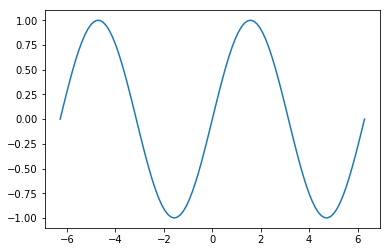
\includegraphics[width=0.5\linewidth,keepaspectratio]{44}
\end{center}
\end{frame}

%%%%%%%%%%%%%%%%%%%%%%%%%%%%%%%%%%%%%%%%%%%%%%%%%%%%%%%%%%%%%%%%%%%%%%%%%%%%%%%%%%%
\begin{frame}[fragile]\frametitle{Saving your Figure}

    Append this to the end of your script:
    \begin{lstlisting}
plt.savefig('myplot.pdf')
    \end{lstlisting}
    It usually figures out the file type from the extension.
    \\~\\
    To remove space around the plot, use:
    \begin{lstlisting}
plt.savefig('myplot.pdf', bbox_inches='tight')
    \end{lstlisting}

\end{frame}

%%%%%%%%%%%%%%%%%%%%%%%%%%%%%%%%%%%%%%%%%%%%%%%%%%%%%%%%%%%%%%%%%%%%%%%%%%%%%%%%%%%
\begin{frame}[fragile]\frametitle{Multiple Plots}

    Plot three sine curves with different phase shifts:
    $y_n = \sin(x + \phi_n)$
    \\~\\
    Call \lstinline|plot()| three times, then \lstinline|show()| the results
    \begin{lstlisting}
import numpy as np
import matplotlib.pyplot as plt

x = np.linspace(-2.*np.pi, 2.*np.pi, 100)
phase = np.arange(0., 2*np.pi, 2*np.pi/3.)

y_n = [np.sin(x + p) for p in phase]

for y in y_n:
    plt.plot(x, y)
plt.show()
    \end{lstlisting}
\begin{center}
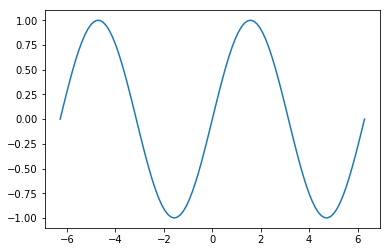
\includegraphics[width=0.25\linewidth,keepaspectratio]{46}
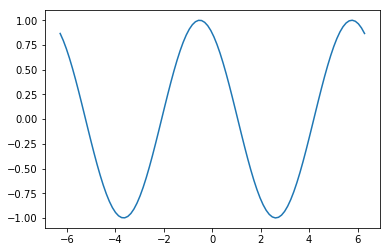
\includegraphics[width=0.25\linewidth,keepaspectratio]{46_1}
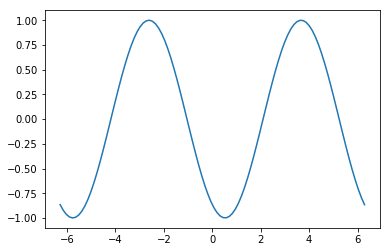
\includegraphics[width=0.25\linewidth,keepaspectratio]{46_2}
\end{center}
\end{frame}

%%%%%%%%%%%%%%%%%%%%%%%%%%%%%%%%%%%%%%%%%%%%%%%%%%%%%%%%%%%%%%%%%%%%%%%%%%%%%%%%%%%
\begin{frame}[fragile]\frametitle{Dots and Dashes}

    Stylise curves with dashes, shapes, and colours (like Matlab):
    \begin{lstlisting}
import numpy as np
import matplotlib.pyplot as plt

x = np.linspace(-2.*np.pi, 2.*np.pi, 50)
phase = np.arange(0., 2*np.pi, 2*np.pi/3.)

y_p = [np.sin(x + p) for p in phase]
style = ['r:', 'g--', 'py']

pdata = zip(y_p, style)
for y,s in pdata:
    plt.plot(x, y, s)
plt.show()
    \end{lstlisting}
\begin{center}
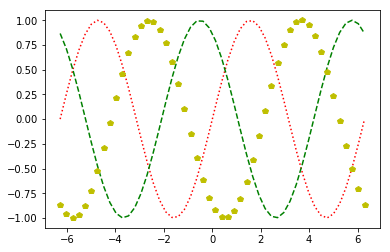
\includegraphics[width=0.25\linewidth,keepaspectratio]{47}
\end{center}
\end{frame}

%%%%%%%%%%%%%%%%%%%%%%%%%%%%%%%%%%%%%%%%%%%%%%%%%%%%%%%%%%%%%%%%%%%%%%%%%%%%%%%%%%%
\begin{frame}[fragile]
    \frametitle{Axis Labels}

    Labeling axes is similar to Matlab:
    \begin{lstlisting}
import numpy as np
import matplotlib.pyplot as plt

x = np.linspace(-2.*np.pi, 2.*np.pi, 100)
phase = np.arange(0., 2*np.pi, 2*np.pi/3.)
y_n = [np.sin(x + p) for p in phase]

for y in y_n:
    plt.plot(x, y)

plt.title('Three-phase plots')
plt.xlabel('x')
plt.ylabel('y')
plt.show()
    \end{lstlisting}
\begin{center}
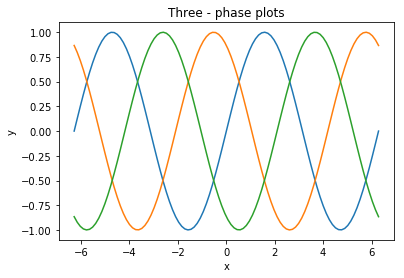
\includegraphics[width=0.25\linewidth,keepaspectratio]{48}
\end{center}
\end{frame}
%%%%%%%%%%%%%%%%%%%%%%%%%%%%%%%%%%%%%%%%%%%%%%%%%%%%%%%%%%%%%%%%%%%%%%%%%%%%%%%%%%%
\begin{frame}[fragile]\frametitle{Legends}

    Include a legend in your plot
    \begin{lstlisting}
import numpy as np
import matplotlib.pyplot as plt

x = np.linspace(-2.*np.pi, 2.*np.pi, 100)
phase = np.arange(0., 2*np.pi, 2*np.pi/3.)
y_n = [np.sin(x + p) for p in phase]

for y in y_n:
    plt.plot(x, y)

legend_text = ['$\phi$ = %.2f' % p
                            for p in phase]
plt.legend(legend_text)
plt.show()
    \end{lstlisting}
\begin{center}
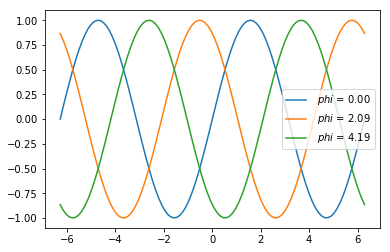
\includegraphics[width=0.25\linewidth,keepaspectratio]{49}
\end{center}
\end{frame}

%%%%%%%%%%%%%%%%%%%%%%%%%%%%%%%%%%%%%%%%%%%%%%%%%%%%%%%%%%%%%%%%%%%%%%%%%%%%%%%%%%%
\begin{frame}[fragile]\frametitle{Contour Plots}

    Plot contours on range $[-2,2]\times[-2,2]$ for the function:
    \[ z(x, y) = \left(x - \frac{1}{2}\right) e^{-\sqrt(x^2 + y^2)} \]
    \begin{lstlisting}
import numpy as np
import matplotlib.pyplot as plt
x_ax = np.linspace(-2., 2., 100)
y_ax = np.linspace(-2., 2., 100)
x, y = np.meshgrid(x_ax, y_ax)
z = (x - 0.5)*np.exp(-np.sqrt(x**2 + y**2))
plt.contour(x, y, z, 25)
plt.show()
    \end{lstlisting}
\begin{center}
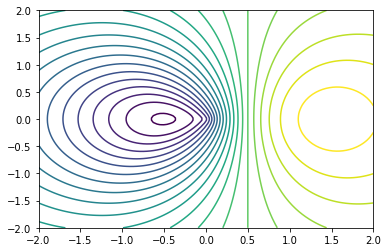
\includegraphics[width=0.25\linewidth,keepaspectratio]{50}
\end{center}
\end{frame}

%%%%%%%%%%%%%%%%%%%%%%%%%%%%%%%%%%%%%%%%%%%%%%%%%%%%%%%%%%%%%%%%%%%%%%%%%%%%%%%%%%%
\begin{frame}[fragile]
    \frametitle{Image Plots}

    \lstinline|imshow| plots pixel fields (\lstinline|pcolor| is very slow)
    \begin{lstlisting}
import numpy as np
import matplotlib.pyplot as plt
x_ax = np.linspace(-2., 2., 100)
y_ax = np.linspace(-2., 2., 100)
x, y = np.meshgrid(x_ax, y_ax)
z = (x-0.5) * np.exp(-np.sqrt(x**2 + y**2))
z_ext = (x_ax[0], x_ax[-1], y_ax[0], y_ax[-1])
plt.imshow(z, origin='lower', extent=z_ext)
plt.show()
    \end{lstlisting}
\begin{center}
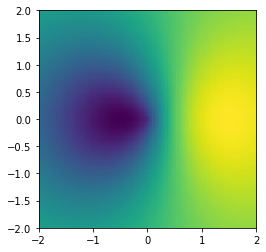
\includegraphics[width=0.25\linewidth,keepaspectratio]{51}
\end{center}
\end{frame}

%%%%%%%%%%%%%%%%%%%%%%%%%%%%%%%%%%%%%%%%%%%%%%%%%%%%%%%%%%%%%%%%%%%%%%%%%%%%%%%%%%%
\begin{frame}[fragile]
    \frametitle{Object-Oriented Matplotlib}
    As your plots become more complex, you may need to start using object-oriented matplotlib
    \begin{lstlisting}
import numpy as np
import matplotlib.pyplot as plt

x = np.linspace(-2.*np.pi, 2.*np.pi, 100)
y = np.sin(x)

fig = plt.figure()
ax = fig.add_subplot(1,1,1)
line = ax.plot(x, y)
ax.set_xlim([-2*np.pi,2*np.pi])

plt.show()
    \end{lstlisting}
\begin{center}
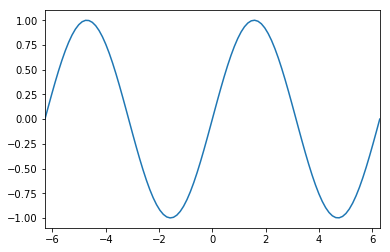
\includegraphics[width=0.25\linewidth,keepaspectratio]{52}
\end{center}
\end{frame}

%%%%%%%%%%%%%%%%%%%%%%%%%%%%%%%%%%%%%%%%%%%%%%%%%%%%%%%%%%%%%%%%%%%%%%%%%%%%%%%%%%%
\begin{frame}[fragile]\frametitle{Subplots}

    Put two plots on the same figure:
    \begin{lstlisting}
import numpy as np
import matplotlib.pyplot as plt

x = np.linspace(-2.*np.pi, 2.*np.pi, 100)
y1 = np.sin(x)
y2 = np.cos(x)

fig, (ax1, ax2) = plt.subplots(nrows=2,
                               ncols=1)
ax1.plot(x, y1)
ax2.plot(x, y2)

plt.show()
    \end{lstlisting}
\begin{center}
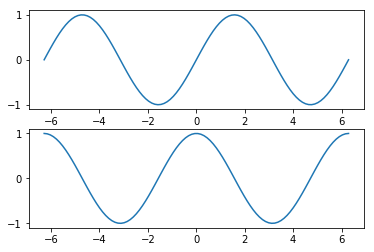
\includegraphics[width=0.25\linewidth,keepaspectratio]{53}
\end{center}
\end{frame}

%%%%%%%%%%%%%%%%%%%%%%%%%%%%%%%%%%%%%%%%%%%%%%%%%%%%%%%%%%%%%%%%%%%%%%%%%%%%%%%%%%%
\begin{frame}[fragile]\frametitle{Basemap: Earth Grid Plotting}

    Basemap provides tools for plotting on several geographic grids.
\end{frame}

%%%%%%%%%%%%%%%%%%%%%%%%%%%%%%%%%%%%%%%%%%%%%%%%%%%%%%%%%%%%%%%%%%%%%%%%%%%%%%%%%%%
\begin{frame}[fragile]\frametitle{Orthographic Grids}
    \begin{lstlisting}
from mpl_toolkits.basemap import Basemap
import numpy as np
import matplotlib.pyplot as plt

m = Basemap(projection='ortho',lon_0=-105,
            lat_0=40,resolution='l')
m.drawcoastlines()
m.fillcontinents(color='coral',
                 lake_color='aqua')
m.drawparallels(np.arange(-90.,120.,30.))
m.drawmeridians(np.arange(0.,420.,60.))
m.drawmapboundary(fill_color='aqua')
plt.show()
    \end{lstlisting}
\end{frame}

%%%%%%%%%%%%%%%%%%%%%%%%%%%%%%%%%%%%%%%%%%%%%%%%%%%%%%%%%%%%%%%%%%%%%%%%%%%%%%%%%%%
\begin{frame}[fragile]\frametitle{Mercator Grids}
    \begin{lstlisting}
from mpl_toolkits.basemap import Basemap
import numpy as np
import matplotlib.pyplot as plt
m = Basemap(projection='merc',llcrnrlat=-80,
            urcrnrlat=80, llcrnrlon=-180,
            urcrnrlon=180,lat_ts=20,
            resolution='c')
m.drawcoastlines()
m.fillcontinents(color='coral',
                 lake_color='aqua')
m.drawparallels(np.arange(-90.,91.,30.))
m.drawmeridians(np.arange(-180.,181.,60.))
m.drawmapboundary(fill_color='aqua')
plt.show()
    \end{lstlisting}
\begin{center}
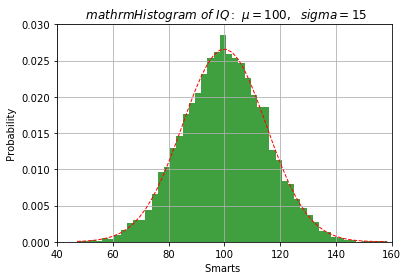
\includegraphics[width=0.25\linewidth,keepaspectratio]{57}
\end{center}
\end{frame}


%%%%%%%%%%%%%%%%%%%%%%%%%%%%%%%%%%%%%%%%%%%%%%%%%%%%%%%%%%%%%%%%%%%%%%%%%%%%%%%%%%%
\begin{frame}[fragile]\frametitle{\emph{Vectors} and \emph{Complex Numbers}}

\begin{lstlisting}
import numpy as np
import matplotlib.mlab as mlab
import matplotlib.pyplot as plt

mu, sigma = 100, 15
x = mu + sigma*np.random.randn(10000)
# the histogram of the data
n, bins, patches = plt.hist(x, 50, normed=1, facecolor='green', 
alpha=0.75)
# add a 'best fit' line
y = mlab.normpdf( bins, mu, sigma)
l = plt.plot(bins, y, 'r--', linewidth=1)
plt.xlabel('Smarts')
plt.ylabel('Probability')
plt.title(r'$\mathrm{Histogram\ of\ IQ:}\ \mu=100,\ \sigma=15$')
plt.axis([40, 160, 0, 0.03])
plt.grid(True)
plt.show()
\end{lstlisting}

\end{frame}

%%%%%%%%%%%%%%%%%%%%%%%%%%%%%%%%%%%%%%%%%%%%%%%%%%%%%%%%%%%%%%%%%%%%%%%%%%%%%%%%%%%
\begin{frame}[fragile]\frametitle{\emph{Vectors} and \emph{Complex Numbers}}
\begin{center}
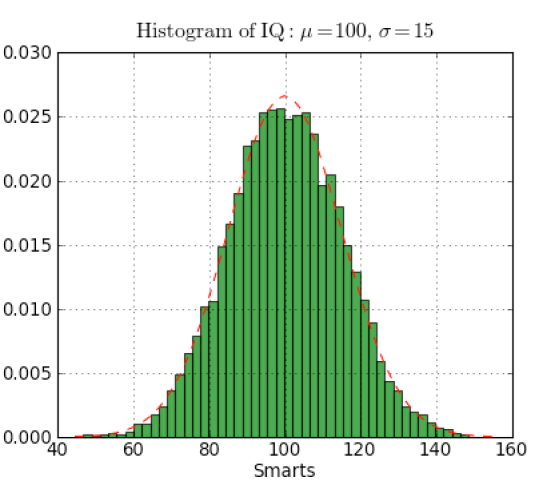
\includegraphics[width=0.75\linewidth,keepaspectratio]{matplotlibhist}
\end{center}
\end{frame}
 
\section[LibII]{Module 9: Libraries II}
%%%%%%%%%%%%%%%%%%%%%%%%%%%%%%%%%%%%%%%%%%%%%%%%%%%%%%%%%%%%%%%%%%%%%%%%%%%%%%%%%%
\begin{frame}[fragile]\frametitle{}
\begin{center}
{\Large Data Mining}
\end{center}
\end{frame}


%%%%%%%%%%%%%%%%%%%%%%%%%%%%%%%%%%%%%%%%%%%%%%%%%%%%%%%%%%%%%%%%%%%%%%%%%%%%%%%%%%%%
%\begin{frame}[fragile]\frametitle{Data, Data, Everywhere}
%	 \begin{itemize}
%		\item The Famous Five:\\\normalsize
%					  Aural, Visual, Somatic, Gustatory, Olfactory		
%		\item The Social Famous Five:\\\normalsize
%					  What people (like to) hear, see, sense, smell, taste, \ldots
%		\item Manifest Data:\\\normalsize
%					  Likes, Ratings, Reviews, Comments, Views, Searches \ldots
%		\item Data about data:\\\normalsize
%					  Location of a tweet, photo, who called whom, \ldots
%		\item Social data:\\\normalsize
%					  Friend graph, followers, who retweeted, liked,\ldots
%		\item Data about structure:\\\normalsize\vspace{-.4\baselineskip} Layout of the site, In/out links, \ldots 
%	\end{itemize}
%\end{frame}
%	
%%%%%%%%%%%%%%%%%%%%%%%%%%%%%%%%%%%%%%%%%%%%%%%%%%%%%%%%%%%%%%%%%%%%%%%%%%%%%%%%%%%%
%\begin{frame}[fragile]
%	\frametitle{Collecting Digital Data}
%	 \begin{itemize}
%		 \item Proprietary Data collections\\\normalsize
%		 			 Lexis-Nexis, comScore \ldots
%		 \item APIs	\\\normalsize
%		 			 Facebook, \href{http://developer.nytimes.com/docs}{NY Times}, Twitter, Google, FourSquare, \href{dfr.jstor.org}{Jstor}, Zillow \ldots
%	 	 \item Bulk Downloads \\\normalsize
%		 			 Wikipedia, data.gov, IMDB, Million Song Database,  Google n-grams \ldots
%		 \item Scraping
%		 \item Custom Apps\\\normalsize Build custom apps to observe behavior, get (pay) people to download these apps
%	 \end{itemize}
%\end{frame}

%%%%%%%%%%%%%%%%%%%%%%%%%%%%%%%%%%%%%%%%%%%%%%%%%%%%%%%%%%%%%%%%%%%%%%%%%%%%%%%%%%%
\begin{frame}[fragile]
	\frametitle{Scraping}
	 \begin{itemize}
		 \item To analyze data, we typically need structure.\\\normalsize 
		 			  For instance, same number of rows for each column.
		 \item But found data often with human readable structure.
		 \item Copy and paste, type, to a dataset.
		 \item But error prone, and not scalable. 
		 \item \alert{Idea:} Find the less accessible structure, automate based on it.  
	 \end{itemize}
\end{frame}

%%%%%%%%%%%%%%%%%%%%%%%%%%%%%%%%%%%%%%%%%%%%%%%%%%%%%%%%%%%%%%%%%%%%%%%%%%%%%%%%%%%%
%\begin{frame}[fragile]
%	\frametitle{Collecting Found Digital Data}
%	\begin{itemize}
%	 \item Software
%	 			\begin{itemize}
%	 			\item R - Not the best but will do.
%				\item Python, Ruby, Perl, Java, \ldots
%				\item 30 Digits, 80 Legs, Grepsr \ldots
%				\end{itemize}
%	  \item Some things to keep in mind
%	  			\begin{itemize}
%	 			\item Check if there is an API, or if data are available for download
%	 			\item Play Nice: \\
%	 						- Scraper may be disallowed in `robots.txt' \\ 
%	 						- Build lag between requests. \alert{Make lags random.}\\
%	 						- Scrape during off-peak hours
%	 			\end{itemize}
%	 \end{itemize}
%	 			
%\end{frame}
%
%%%%%%%%%%%%%%%%%%%%%%%%%%%%%%%%%%%%%%%%%%%%%%%%%%%%%%%%%%%%%%%%%%%%%%%%%%%%%%%%%%%%
%\begin{frame}[fragile]
%\frametitle{Paper}
%
%	\begin{itemize}
%	\item  Create digital images of paper
%	\item  Identify colored pixels as characters (OCR) 
%	\item  Software
%		\begin{itemize}
%		 \item Adobe Pro., etc. 
%		 \item Best in class commercial: Abbyy FineReader \\
%		 			  Now has an API 
%	 	 \item Best in class open-source: Tesseract
%		\end{itemize}
%	\item Scrape off recognized characters: pyPdf etc.
%	\item Post-processing
%	\end{itemize}
%
%\end{frame}
%
%%%%%%%%%%%%%%%%%%%%%%%%%%%%%%%%%%%%%%%%%%%%%%%%%%%%%%%%%%%%%%%%%%%%%%%%%%%%%%%%%%%%
%\begin{frame}[fragile]
%\frametitle{Pictures, Audio, and Video}
%	\begin{itemize}
%		\item Audio (or Video with audio) to text: Dragon Dictates, Google transcription 
%		\item Pictures: recognize color, faces 
%		\item Objects in images: \href{clarifai.com}{Clarifai}
%		\item Scrape closed-captions
%	\end{itemize}
%\end{frame}
%
%%%%%%%%%%%%%%%%%%%%%%%%%%%%%%%%%%%%%%%%%%%%%%%%%%%%%%%%%%%%%%%%%%%%%%%%%%%%%%%%%%%%
%\begin{frame}[fragile]
%\frametitle{Get Others to Work}
%	\begin{itemize}
%		\item Human Computing
%		\item Amazon.com's Mechanical Turk
%			\begin{itemize}
%				\item  Create Human Intensive Tasks (HITs)
%				\item  \href{https://www.mturk.com/mturk/findhits?match=false}{Surveys, transcription, translation, \ldots}
%				\item  You assess the work and pay out 
%			\end{itemize}
%		\item Odesk, elance, impact sourcing, run your own ads \ldots
%		\item \href{http://www.google.com/insights/consumersurveys/home}{Google} -- surveys as payment for content
%\end{itemize}
%
%\end{frame}
%
%%%%%%%%%%%%%%%%%%%%%%%%%%%%%%%%%%%%%%%%%%%%%%%%%%%%%%%%%%%%%%%%%%%%%%%%%%%%%%%%%%%%
%\begin{frame}[fragile]
%\frametitle{Scraping one HTML page in Python} 
%
%Shakespeare's Twelfth Night\\
%Using \href{http://www.crummy.com/software/BeautifulSoup/}{Beautiful Soup}
%\small
%	\begin{itemize}
%		\item  \lstinline| from BeautifulSoup import BeautifulSoup|
%		\item  \lstinline| from urllib import urlopen|
%		\item 
%		\item  \lstinline| url  = urlopen(`http://bit.ly/1D7wKcH').read()|
%		\item  \lstinline| soup = BeautifulSoup(url)|
%		\item  \lstinline| text = soup.p.contents|
%		\item  \lstinline| print text|
%	\end{itemize}
%\end{frame}
%
%%%%%%%%%%%%%%%%%%%%%%%%%%%%%%%%%%%%%%%%%%%%%%%%%%%%%%%%%%%%%%%%%%%%%%%%%%%%%%%%%%%%
%\begin{frame}[fragile]
%\frametitle{Getting text from one pdf in Python} 
%
%A Political Ad\\
%Using \href{http://pybrary.net/pyPdf/}{PyPdf}
%\small
%	\begin{itemize}
%		\item  \lstinline| import pyPdf|
%		\item 
%		\item  \lstinline| pdf = pyPdf.PdfFileReader(file('path to pdf', `rb'))|
%		\item  \lstinline| content = pdf.getPage(0).extractText()|
%		\item  \lstinline| print content|
%	\end{itemize}
%\end{frame}

%%%%%%%%%%%%%%%%%%%%%%%%%%%%%%%%%%%%%%%%%%%%%%%%%%%%%%%%%%%%%%%%%%%%%%%%%%%%%%%%%%%%
%\begin{frame}[fragile]
%	\frametitle{Scraping many urls/files to structured data}
%	\begin{itemize}
%		\item Loop, exploiting structure of the urls/file paths\\\normalsize 
%					 e.g. \href{http://search.espncricinfo.com/ci/content/match/search.html?search=odi;all=1;page=1}{ESPN URL}
%		\item Handle errors, if files or urls don't open, what do you do?
%		\item To harvest structured data, exploit structure within text
%		\item Trigger words, html tags, \ldots 
%	\end{itemize}
%\end{frame}

%%%%%%%%%%%%%%%%%%%%%%%%%%%%%%%%%%%%%%%%%%%%%%%%%%%%%%%%%%%%%%%%%%%%%%%%%%%%%%%%%%%%
%\begin{frame}[fragile]
%	\frametitle{Exception(al) Handling}
%	\begin{itemize}
%		\item  \lstinline|try:|
%		\item  \lstinline|     pdf = pyPdf.PdfFileReader(file(pdfFile, 'rb'))|
%		\item  \lstinline|except Exception, e:|
%		\item  \lstinline|     return `Cannot Open: {} with error: {}'.format(pdfFile, str(e))|
%	\end{itemize}
%\end{frame}

%%%%%%%%%%%%%%%%%%%%%%%%%%%%%%%%%%%%%%%%%%%%%%%%%%%%%%%%%%%%%%%%%%%%%%%%%%%%%%%%%%%%
%\begin{frame}[fragile]
%	\frametitle{Inside the page}
%	\begin{itemize}
%		\item Chrome Developer Tools
%		\item Quick Tour of HTML
%			\begin{itemize}
%			\item Tags begin with < and end with >
%			\item Tags usually occur in pairs. Some don't (see img). And can be nested.
%			\item \href{https://developer.mozilla.org/en-US/docs/Web/HTML/Element}{Mozilla HTML elements}
%			\item <p> is for paragraph
%			\item <a> is for a link
%			\item <ol>, <ul> is for ordered, unordered list; <li> is a bullet
%			\item tags can have attributes. <a href='http://somesite'></a>
%			\item DOM, hierarchical, parent, child:
%\begin{lstlisting}
%<html>
%    <body>
%        <p></p> 
%    </body>
%</html>
%\end{lstlisting}
%		\end{itemize}
%	\end{itemize}
%\end{frame}
%
%%%%%%%%%%%%%%%%%%%%%%%%%%%%%%%%%%%%%%%%%%%%%%%%%%%%%%%%%%%%%%%%%%%%%%%%%%%%%%%%%%%%
%\begin{frame}[fragile]
%	\frametitle{Find Things}
%	\begin{itemize}
%		\item Navigate by HTML tags:  \lstinline| soup.title, soup.body, soup.body.contents|
%		\item Search HTML tags: 	   \lstinline| soup.find_all('a'), soup.find(id="nav1")|
%		\item 
%		\item So to get all the urls in a page:
%		\item  \lstinline| for link in soup.find_all('a'):|
%		\item  \lstinline|      print(link.get('href'))	|						
%		\item 
%		\item \href{http://www.crummy.com/software/BeautifulSoup/bs4/doc/}{Beautiful Soup Documentation}
%	\end{itemize}
%\end{frame}
%
%%%%%%%%%%%%%%%%%%%%%%%%%%%%%%%%%%%%%%%%%%%%%%%%%%%%%%%%%%%%%%%%%%%%%%%%%%%%%%%%%%%%
%\begin{frame}[fragile]
%	\frametitle{Data Munging}
%	\Large
%		``Data scientists, according to interviews and expert estimates, spend from \alert{50 percent to 80 percent of their time mired in the mundane labor of collecting and preparing data}, before it can be explored for useful information.''\\\vspace{5em}
%
%		\small \href{http://www.nytimes.com/2014/08/18/technology/for-big-data-scientists-hurdle-to-insights-is-janitor-work.html}{New York Times: For BigData Scientists, `Janitor Work' Is Key Hurdle to Insights}
%
%\end{frame}
%
%%%%%%%%%%%%%%%%%%%%%%%%%%%%%%%%%%%%%%%%%%%%%%%%%%%%%%%%%%%%%%%%%%%%%%%%%%%%%%%%%%%%
%\begin{frame}[fragile]
%	\frametitle{Data Munging}
%	\Large
%	``In our experience, the tasks of \alert{exploratory data mining and data cleaning constitute 80\% of the effort} that determines 80\% of the value of the ultimate data.''\\\vspace{5em}
%
%	\small Dasu and Johnson, Exploratory Data Mining and Data Cleaning
%\end{frame}
%
%%%%%%%%%%%%%%%%%%%%%%%%%%%%%%%%%%%%%%%%%%%%%%%%%%%%%%%%%%%%%%%%%%%%%%%%%%%%%%%%%%%%
%\begin{frame}[fragile]
%	\frametitle{Regular (or Rational) Expressions}
%	\begin{itemize}
%		\item  Formal language for specifying text strings
%		\item  Stephen Kleene, `inventor' of regular expressions.
%		\item  Henry Spencer, behind the {\tt regex} library.
%		\item  Descend from {\it finite automata} theory.
%		\item  Matching
%	\end{itemize}
%\end{frame}
%
%%%%%%%%%%%%%%%%%%%%%%%%%%%%%%%%%%%%%%%%%%%%%%%%%%%%%%%%%%%%%%%%%%%%%%%%%%%%%%%%%%%%
%\begin{frame}[fragile]
%	\frametitle{The most basic regular expression}
%	\begin{itemize}
%		\item String literal
%		\item \href{http://regexpal.com}{RegexPal.com}
%		\item Say you are searching for the word apple -- can be uppercase first character, plural, lowercase first character
%	\end{itemize}
%\end{frame}
%
%%%%%%%%%%%%%%%%%%%%%%%%%%%%%%%%%%%%%%%%%%%%%%%%%%%%%%%%%%%%%%%%%%%%%%%%%%%%%%%%%%%%
%\begin{frame}[fragile]
%	\frametitle{Disjunction}
%	\begin{itemize}
%		\item Disjunction, Character classes
%				\begin{itemize}
%				\item   \lstinline| []|
%				\item   \lstinline| [aA]pple matches apple and Apple|
%				\item   \lstinline| [0123456789]  matches any digit|
%				\end{itemize}
%		\item Ranges
%			\begin{itemize}
%				\item   \lstinline| [0-9]  matches any digit|
%				\item   \lstinline| [a-z], [[:lower:]]  matches any lowercase|
%				\item   \lstinline| [a-zA-Z], [[:alpha:]]  matches any uppercase|
%				\item   \lstinline| [a-e1-9]  matches any letter or digit|
%				\item  Hyphen only has a special meaning if used within range.  \lstinline| [-123]|
%			\end{itemize}
%	\end{itemize}
%\end{frame}
%
%%%%%%%%%%%%%%%%%%%%%%%%%%%%%%%%%%%%%%%%%%%%%%%%%%%%%%%%%%%%%%%%%%%%%%%%%%%%%%%%%%%%
%\begin{frame}[fragile]
%	\frametitle{Disjunction Contd..}
%	\begin{itemize}
%	\item Negation in Disjunction\\\normalsize
%			\begin{itemize}
%			\item   \lstinline| ^ right after the square bracket means a negation|
%			\item   \lstinline|  [^A-Z]|
%			\item   \lstinline|  [^Aa] means neither a capital A nor a lowercase a|
%			\item   \lstinline|  [^e^] means not an e, and not ^|
%			\end{itemize}
%	\item Disjunction for longer strings\\\normalsize
%			\begin{itemize}
%			    \item   \lstinline|  pipe|
%				\item   \lstinline|  a|b|c = [abc]|
%				\item   \lstinline|  apple|pie|
%				\item   \lstinline|  [aA]pple|[aA]nd|
%			\end{itemize}
%	\end{itemize}
%\end{frame}
%
%%%%%%%%%%%%%%%%%%%%%%%%%%%%%%%%%%%%%%%%%%%%%%%%%%%%%%%%%%%%%%%%%%%%%%%%%%%%%%%%%%%%
%\begin{frame}[fragile]
%	\frametitle{Special characters}
%	\begin{itemize}
%	\item ? - previous character is optional: colou?r - color, colour
%	\item  . matches any character\\
%				  e.g. beg.n matches begun, begin, began
%	\item Kleene Operators - named after Steven Kleene
%			\begin{itemize}
%			\item *  matches 0 or more of the previous characters\\
%						e.g. oo*h will match ooh, oooh, etc.\\
%						(abc)* will match abc, abcabc, etc.
%			\item +  matches 1 or more of the previous characters\\
%						e.g. o+h will match ooh, oooh, etc. 
%			\end{itemize}
%	\end{itemize}
%\end{frame}
%
%%%%%%%%%%%%%%%%%%%%%%%%%%%%%%%%%%%%%%%%%%%%%%%%%%%%%%%%%%%%%%%%%%%%%%%%%%%%%%%%%%%%
%\begin{frame}[fragile]
%	\frametitle{Repetition Ranges}
%	\begin{itemize}
%	\item  Specific ranges can also be specified
%	\item  \small  \lstinline| { } to specify range for the immediately preceding regex|
%	\item   \lstinline| {n}  means exactly n occurrences|
%	\item   \lstinline| {n,} means at least n occurrences|
%	\item   \lstinline| {n,m} means at least n and no more than m occurrences|
%	\item  Example:  \lstinline| . {0, } = .*|	
%	\end{itemize}
%\end{frame}
%
%%%%%%%%%%%%%%%%%%%%%%%%%%%%%%%%%%%%%%%%%%%%%%%%%%%%%%%%%%%%%%%%%%%%%%%%%%%%%%%%%%%%
%\begin{frame}[fragile]\frametitle{More Regex}
%		\begin{itemize}
%	\item Anchors
%			\begin{itemize}
%			\item  \^ matches the beginning of the line \\
%	 			  e.g.  \lstinline| ^[A-Z] matches a capital letter at the start of a line.|
%			\item  \$ matches the end of the line.
%			\end{itemize}
%	\item   \lstinline| \. means a period| 
%	\item  Example: look for the word `the'
%	\begin{itemize}
%		\item missed capitalization: [tT]he
%		\item make pattern more precise: \\
%					 \lstinline| [tT]he[^A-Za-z], ^[tT]he[^A-Za-z]|
%	\end{itemize}
%	\end{itemize}
%\end{frame}
%
%%%%%%%%%%%%%%%%%%%%%%%%%%%%%%%%%%%%%%%%%%%%%%%%%%%%%%%%%%%%%%%%%%%%%%%%%%%%%%%%%%%%
%\begin{frame}[fragile]
%\frametitle{False Positive and Negatives}
%	\begin{itemize}
%	\item False positives or Type 1 errors - matching things we shouldn't match
%	\item False negatives or Type 2 errors - not matching things we should match
%	\item Cost attached to false negative and positive
%	\item Provide some metrics by comparing against good data for a small sample
%	\end{itemize}
%\end{frame}
%
%%%%%%%%%%%%%%%%%%%%%%%%%%%%%%%%%%%%%%%%%%%%%%%%%%%%%%%%%%%%%%%%%%%%%%%%%%%%%%%%%%%%
%\begin{frame}[fragile]
%	\frametitle{Edit Distance}
%	\begin{itemize}
%		\item pwned -> owned or pawned?
%		\item standd -> strand, stand, stood, or sand?
%		\item How similar are two strings?
%		\item Applications
%			\begin{itemize}
%			\item Spell Correction
%			\item Also comes up in computational biology
%			\item Machine translation
%			\item Information extraction
%			\item Speech recognition
%			\end{itemize}
%	\end{itemize}
%\end{frame}
%
%%%%%%%%%%%%%%%%%%%%%%%%%%%%%%%%%%%%%%%%%%%%%%%%%%%%%%%%%%%%%%%%%%%%%%%%%%%%%%%%%%%%
%\begin{frame}[fragile]
%	\frametitle{Edit Distance}
%	\begin{itemize}
%		\item Typically refers to minimum edit distance
%		\item Minimum number of editing operations to convert one string to another
%			\begin{itemize}
%				\item Insertion
%				\item Deletion
%				\item Substitution
%			\end{itemize}
%		\item e.g. two strings: intention, execution 
%			\begin{itemize}
%				\item align it with second letter
%				\item d (delete), s (substitute), s, i(nsert), s
%				\item if each operation costs 1, edit distance = 5
%				\item if substitition cost 2 (levenshtein distance), distance = 8
%			\end{itemize}
%		\item You can implement this at word level so Microsoft Corp. is 1 away from Microsoft.
%	\end{itemize}
%\end{frame}
%
%%%%%%%%%%%%%%%%%%%%%%%%%%%%%%%%%%%%%%%%%%%%%%%%%%%%%%%%%%%%%%%%%%%%%%%%%%%%%%%%%%%%
%\begin{frame}[fragile]
%	\frametitle{Text as Data}
%	\begin{itemize}
%		\item Bag of words assumption\\\normalsize
%					Lose word order
%		\item Remove stop words:\\\normalsize
%					If, and, but, who, what, the, they, their, a, or, \ldots\\
%					\alert{Be careful: one person's stopword is another's key term.}
%		\item (Same) Word: Stemming and Lemmatization\\\normalsize
%					Taxing, taxes, taxation, taxable $\leadsto$ tax
%		\item Remove rare words\\\normalsize
%					$\sim$ .5\% to 15\%, depending on application\\
%		\item Convert to lowercase, drop numbers, punctuation, etc.
%	\end{itemize}
%\end{frame}
%
%%%%%%%%%%%%%%%%%%%%%%%%%%%%%%%%%%%%%%%%%%%%%%%%%%%%%%%%%%%%%%%%%%%%%%%%%%%%%%%%%%%%
%\begin{frame}[fragile]
%	\frametitle{How?}
%	Using Natural Language Toolkit (\tt{nltk})
%	\begin{itemize}
%			\item \textbf{Lowercase}: 
% 					 	 \lstinline|text = text.lower()| 
% 			\item \textbf{Remove stop words}:
%	 			\item  \lstinline|swords = stopwords.words('english')|
%	 			\item  \lstinline|words  = wordpunct_tokenize(text)|
%	 			\item  \lstinline|words  = [w for w in words if w not in swords]|
%	    		\item  \lstinline|text = ' '.join(words)|
% 			\item \textbf{Stemming}: 
% 				\item  \lstinline|st = EnglishStemmer()|
% 				\item  \lstinline|words = wordpunct_tokenize(text)|
%    			\item  \lstinline|words = [st.stem(w) for w in words]|
%    			\item  \lstinline|text = ' '.join(words)|
%		\end{itemize}
%\end{frame}
%
%%%%%%%%%%%%%%%%%%%%%%%%%%%%%%%%%%%%%%%%%%%%%%%%%%%%%%%%%%%%%%%%%%%%%%%%%%%%%%%%%%%%
%\begin{frame}[fragile]
%	\frametitle{To Matrices}
%	\begin{itemize}
%			\item n-grams
%					 \lstinline|
%						from nltk import bigrams, trigrams, ngrams
%						text = word tokenize(text)
%						text_bi  = bigrams(text)
%					|
%	\end{itemize}
%\end{frame}

%%%%%%%%%%%%%%%%%%%%%%%%%%%%%%%%%%%%%%%%%%%%%%%%%%%%%%%%%%%%%%%%%%%%%%%%%%%%%%%%%%%
\begin{frame}[fragile]\frametitle{Web Scraping Workflow}
Web scraping downloads and processes content from the Web
\begin{itemize}
\item Get the website - using HTTP library
\item Parse the html document - using any parsing library
\item Store the results - either a db, csv, text file, etc
\end{itemize}
Libraries:
\begin{itemize}
\item \textbf{Requests}: Downloads files and web pages from the Internet
\item \textbf{Beautiful Soup}: Parses HTML, the format that web pages are written in.
\item \textbf{Selenium}: To fill in forms and simulate mouse clicks in this browser.
\end{itemize}
\end{frame}

%%%%%%%%%%%%%%%%%%%%%%%%%%%%%%%%%%%%%%%%%%%%%%%%%%%%%%%%%%%%%%%%%%%%%%%%%%%%%%%%%%%
\begin{frame}[fragile]\frametitle{Web Scraping Issues}
Web-scraping is difficult for some annoying (i.e. not particularly intellectually challenging) reasons:
\begin{itemize}
\item Web pages change frequently and will break your code.
\item Web page source code is often not logical and consistent (major browsers are incredibly good at overlooking this, but python and your own code probably aren't).
\item Content may be different for different User Agents (which client you're using).
\item Content may be hidden behind logins, require cookies or other fancier browser options, etc.
\item Websites may attempt to limit automated crawling of their pages (robots.txt) — your code may have to go out of its way to be nice, or risk getting banned.
\end{itemize}
\end{frame}

%%%%%%%%%%%%%%%%%%%%%%%%%%%%%%%%%%%%%%%%%%%%%%%%%%%%%%%%%%%%%%%%%%%%%%%%%%%%%%%%%%%
\begin{frame}[fragile]\frametitle{Web Scraping: Get the website }
Suppose that we want to crawl this web page:
https://www.hkex.com.hk/eng/index.htm

\begin{center}
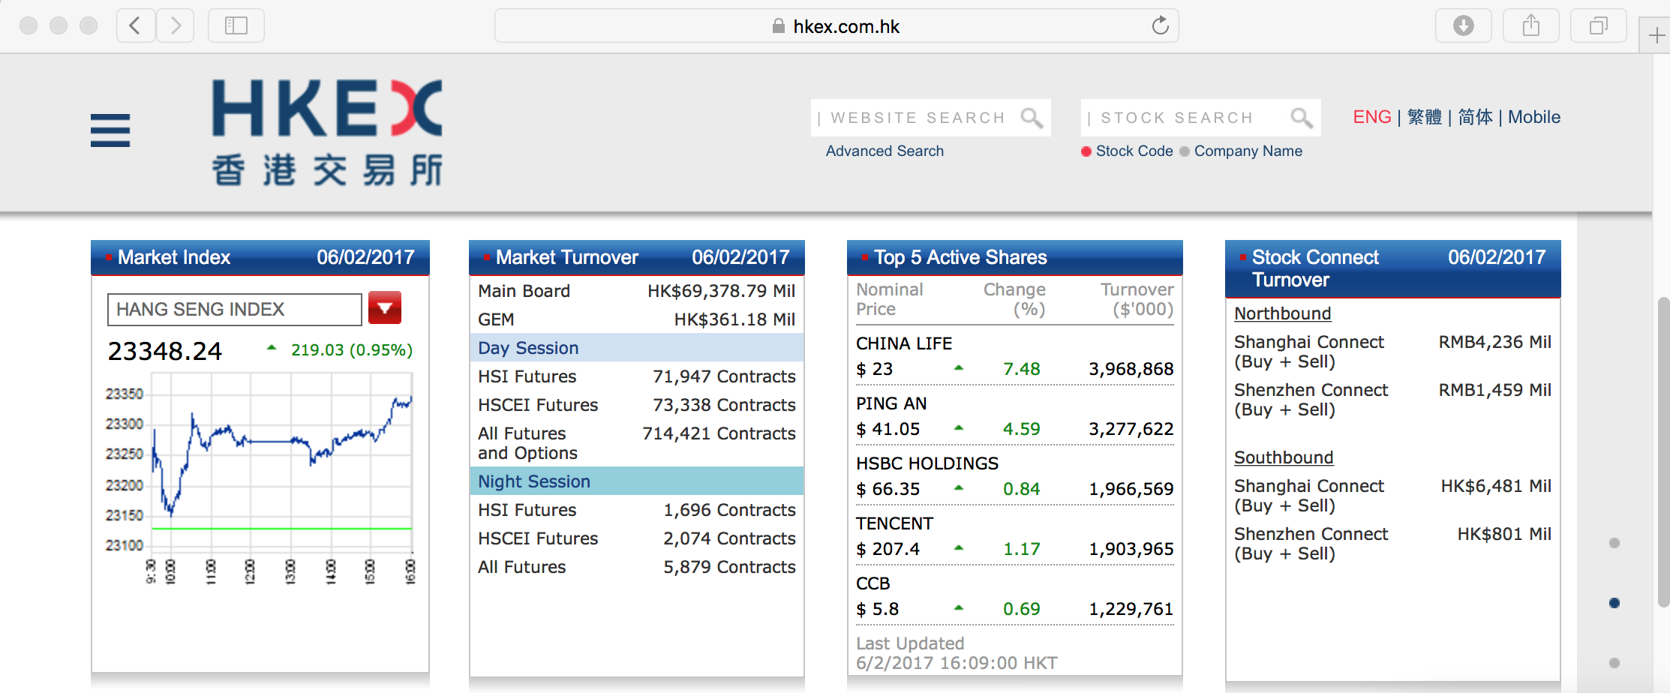
\includegraphics[width=\linewidth,keepaspectratio]{hkex}
\end{center}
\tiny{(Reference: https://studyslide.com/doc/288619/tutorial-2---hkust-cse)}

\end{frame}

%%%%%%%%%%%%%%%%%%%%%%%%%%%%%%%%%%%%%%%%%%%%%%%%%%%%%%%%%%%%%%%%%%%%%%%%%%%%%%%%%%%
\begin{frame}[fragile]\frametitle{Web Scraping: Get the website }
In Chrome: Right-click, choose ``View Page Source''
\begin{center}
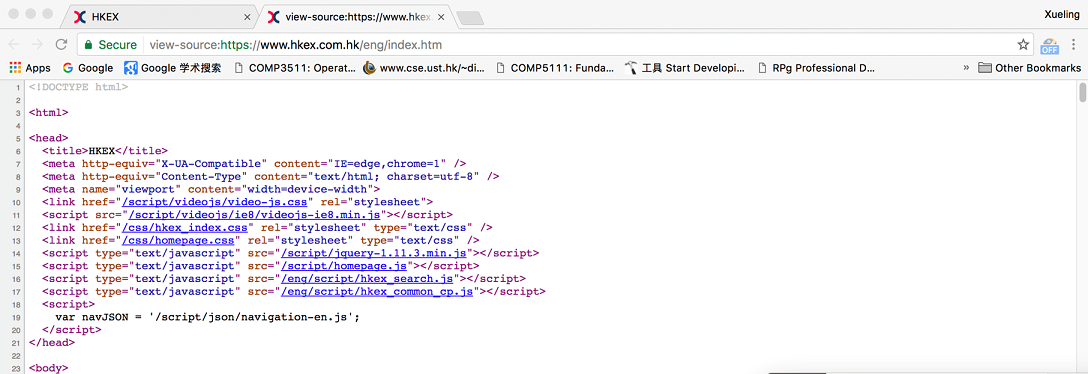
\includegraphics[width=\linewidth,keepaspectratio]{hkexsrc}
\end{center}
\end{frame}

%%%%%%%%%%%%%%%%%%%%%%%%%%%%%%%%%%%%%%%%%%%%%%%%%%%%%%%%%%%%%%%%%%%%%%%%%%%%%%%%%%%
\begin{frame}[fragile]\frametitle{Web Scraping: Get the website }
We need to collect useful information from source HTML code:
\begin{center}
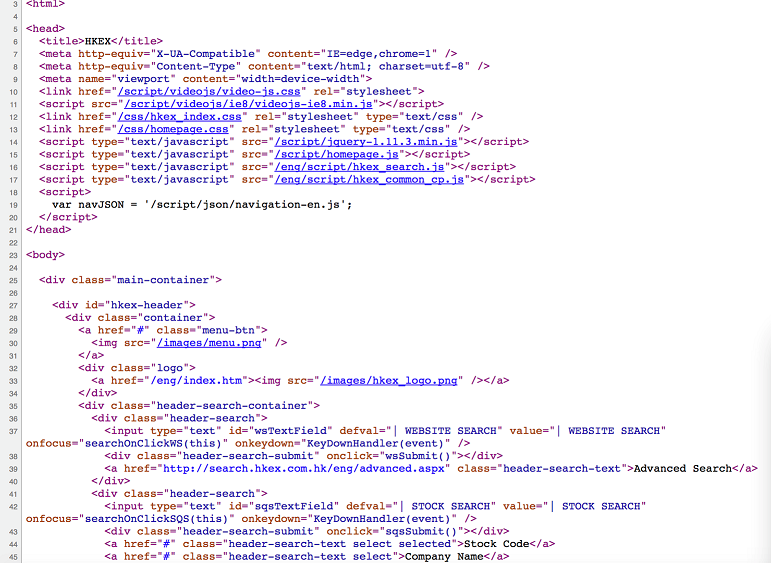
\includegraphics[width=0.8\linewidth,keepaspectratio]{hkexhtml}
\end{center}
\end{frame}


%%%%%%%%%%%%%%%%%%%%%%%%%%%%%%%%%%%%%%%%%%%%%%%%%%%%%%%%%%%%%%%%%%%%%%%%%%%%%%%%%%%
\begin{frame}[fragile]\frametitle{Requests}
Web scraping downloads and processes content from the Web
\begin{itemize}
\item Do not need to worry about complicated issues such as network errors, connection problems, and data compression.
\item \lstinline|requests.get()| function takes a string of a URL to download. 
\begin{lstlisting}
import requests
res = requests.get('https://automatetheboringstuff.com/files/rj.txt')
\end{lstlisting}
\item Response contains the response that the web server gave.
\begin{lstlisting}
if res.status_code == requests.codes.ok:
	print(res.text)
\end{lstlisting}
\end{itemize}
\end{frame}
%%%%%%%%%%%%%%%%%%%%%%%%%%%%%%%%%%%%%%%%%%%%%%%%%%%%%%%%%%%%%%%%%%%%%%%%%%%%%%%%%%%
\begin{frame}[fragile]\frametitle{Beautiful Soup}
Web scraping downloads and processes content from the Web
\begin{itemize}
\item To parse a document, pass it into the BeautifulSoup constructor. You can pass in a string or an open filehandle:

\begin{lstlisting}
from bs4 import BeautifulSoup

soup = BeautifulSoup(open("index.html")) 
soup = BeautifulSoup("<html>data</html>")  
\end{lstlisting}
\item Print the content in the soup object in better format 
\lstinline|print(soup.prettify())|
\item A Tag object corresponds to an XML or HTML tag in the original document:
\lstinline|<title>The Dormouse's story</title>|
\item Use BeautifulSoup to get the tags in a convenient way
\lstinline|print(soup.title)| \\
\lstinline|print(soup.head)|
\end{itemize}

\end{frame}

%%%%%%%%%%%%%%%%%%%%%%%%%%%%%%%%%%%%%%%%%%%%%%%%%%%%%%%%%%%%%%%%%%%%%%%%%%%%%%%%%%%
\begin{frame}[fragile]\frametitle{Beautiful Soup: Tag}
Web scraping downloads and processes content from the Web
\begin{itemize}
\item Every tag has a name, accessible as .name
\begin{lstlisting}
print(soup.head.name)
#head
\end{lstlisting}
\item  A tag may have any number of attributes. The tag \lstinline|<b class=``boldest''>| has an attribute ``class'' whose value is ``boldest''. You can access a tag's attributes by treating the tag like a dictionary:
\begin{lstlisting}
print(soup.p.attrs)
#{'class': ['title'], 'name': 'dromouse'}
print(soup.p['class'])
#['title']
print(soup.p.get('class'))
#['title']
print(type(soup.p))
#<class 'bs4.element.Tag'>
\end{lstlisting}
\end{itemize}

\end{frame}

%%%%%%%%%%%%%%%%%%%%%%%%%%%%%%%%%%%%%%%%%%%%%%%%%%%%%%%%%%%%%%%%%%%%%%%%%%%%%%%%%%%
\begin{frame}[fragile]\frametitle{Beautiful Soup: Sample workflow}

\begin{itemize}
\item To begin, we need to import Beautiful Soup and urllib, and grab source code:
\begin{lstlisting}
import bs4 as bs
import urllib.request

source = urllib.request.urlopen('https://pythonprogramming.net/parsememcparseface/').read()
\end{lstlisting}
\item  Then, we create the ``soup''. This is a beautiful soup object:
\begin{lstlisting}
soup = bs.BeautifulSoup(source,'lxml')
\end{lstlisting}
\item  Find more about whats in the soup object:
\begin{lstlisting}
print(soup.title)
print(soup.title.name)
print(soup.title.string)

# beginning navigation:
print(soup.title.parent.name)

# getting specific values:
print(soup.p)
\end{lstlisting}
\end{itemize}

\end{frame}

%%%%%%%%%%%%%%%%%%%%%%%%%%%%%%%%%%%%%%%%%%%%%%%%%%%%%%%%%%%%%%%%%%%%%%%%%%%%%%%%%%%
\begin{frame}[fragile]\frametitle{Beautiful Soup: Sample workflow}

\begin{itemize}
\item Finding paragraph tags <p> is a fairly common task. What if we wanted to find them all?
\begin{lstlisting}
print(soup.find_all('p'))
\end{lstlisting}
\item  We can also iterate through them:
\begin{lstlisting}
for paragraph in soup.find_all('p'):
    print(paragraph.string)
    print(str(paragraph.text))
\end{lstlisting}
\item  The difference between string and text is that string produces a NavigableString object, and text is just typical unicode text. 
\item  Notice that, if there are child tags in the paragraph item that we're attempting to use .string on, we will get None returned.
\end{itemize}

\end{frame}

%%%%%%%%%%%%%%%%%%%%%%%%%%%%%%%%%%%%%%%%%%%%%%%%%%%%%%%%%%%%%%%%%%%%%%%%%%%%%%%%%%%
\begin{frame}[fragile]\frametitle{Beautiful Soup: Sample workflow}

\begin{itemize}
\item  Another common task is to grab links. For example:
\begin{lstlisting}
for url in soup.find_all('a'):
    print(url.get('href'))
\end{lstlisting}
\item  In this case, if we just grabbed the .text from the tag, you'd get the anchor text, but we actually want the link itself. 
\item  That's why we're using \lstinline|.get('href')| to get the true URL.
\item Finally, you may just want to grab text. You can use \lstinline|.get_text()| on a Beautiful Soup object, including the full soup:
\begin{lstlisting}
print(soup.get_text())
\end{lstlisting}
\end{itemize}
This concludes the introduction to Beautiful Soup. 
\end{frame}

%%%%%%%%%%%%%%%%%%%%%%%%%%%%%%%%%%%%%%%%%%%%%%%%%%%%%%%%%%%%%%%%%%%%%%%%%%%%%%%%%%%
\begin{frame}[fragile]\frametitle{Beautiful Soup: Sample workflow}

\begin{itemize}
\item  Another common task is to grab links. For example:
\begin{lstlisting}
for url in soup.find_all('a'):
    print(url.get('href'))
\end{lstlisting}
\item  In this case, if we just grabbed the .text from the tag, you'd get the anchor text, but we actually want the link itself. 
\item  That's why we're using \lstinline|.get('href')| to get the true URL.
\item Finally, you may just want to grab text. You can use \lstinline|.get_text()| on a Beautiful Soup object, including the full soup:
\begin{lstlisting}
print(soup.get_text())
\end{lstlisting}
\end{itemize}
This concludes the introduction to Beautiful Soup. Next is the Navigation.
\end{frame}


%%%%%%%%%%%%%%%%%%%%%%%%%%%%%%%%%%%%%%%%%%%%%%%%%%%%%%%%%%%%%%%%%%%%%%%%%%%%%%%%%%%
\begin{frame}[fragile]\frametitle{Beautiful Soup: Sample workflow}

\begin{itemize}
\item  In this case, we're grabbing the first nav tags that we can find (the navigation bar):
\begin{lstlisting}
nav = soup.nav
for url in nav.find_all('a'):
    print(url.get('href'))
\end{lstlisting}
\item   You could also go for soup.body to get the body section, then grab the \lstinline|.text| from there:
\begin{lstlisting}
body = soup.body
for paragraph in body.find_all('p'):
    print(paragraph.text)
\end{lstlisting}
\item To avoid multiple tags with same names, use other things such as classes, to differentiate:
\begin{lstlisting}
for div in soup.find_all('div', class_='body'):
    print(div.text)
\end{lstlisting}
\end{itemize}

\end{frame}

%%%%%%%%%%%%%%%%%%%%%%%%%%%%%%%%%%%%%%%%%%%%%%%%%%%%%%%%%%%%%%%%%%%%%%%%%%%%%%%%%%%
\begin{frame}[fragile]\frametitle{Beautiful Soup: Sample workflow}

\begin{itemize}
\item Parsing the table:
\begin{lstlisting}
table = soup.find('table')
\end{lstlisting}
\item   Next, we can find the table rows within the table:
\begin{lstlisting}
table_rows = table.find_all('tr')
\end{lstlisting}
\item Then we can iterate through the rows, find the td tags, and then print out each of the table data tags:
\begin{lstlisting}
for tr in table_rows:
    td = tr.find_all('td')
    row = [i.text for i in td]
    print(row)
\end{lstlisting}
\end{itemize}

\end{frame}








%%%%%%%%%%%%%%%%%%%%%%%%%%%%%%%%%%%%%%%%%%%%%%%%%%%%%%%%%%%%%%%%%%%%%%%%%%%%%%%%%%
\begin{frame}[fragile]\frametitle{}
\begin{center}
{\Large Tkinter}

\tiny{(Reference: CS2316, Fall 2016 http://cs2316.gatech.edu/slides/tkinter.pptx)}

\end{center}
\end{frame}



%%%%%%%%%%%%%%%%%%%%%%%%%%%%%%%%%%%%%%%%%%%%%%%%%%%
\begin{frame}[fragile] \frametitle{GUI: Graphical User Interface}

\adjustbox{valign=t}{
\begin{minipage}{0.45\linewidth}
\begin{itemize}
\item A way for people to interact with computer programs
\item Uses windows, icons and menus
\item Can be manipulated by a mouse and keyboard
\end{itemize}
%\begin{lstlisting}
%x = 2
%y = 3
%op1 = tf.add(x, y)
%op2 = tf.mul(x, y)
%useless = tf.mul(x, op1)
%op3 = tf.pow(op2, op1)
%with tf.Session() as sess:
%    op3 = sess.run(op3)
%
%\end{lstlisting}
\end{minipage}
}
\hfill
\adjustbox{valign=t}{
\begin{minipage}{0.45\linewidth}
\begin{center}
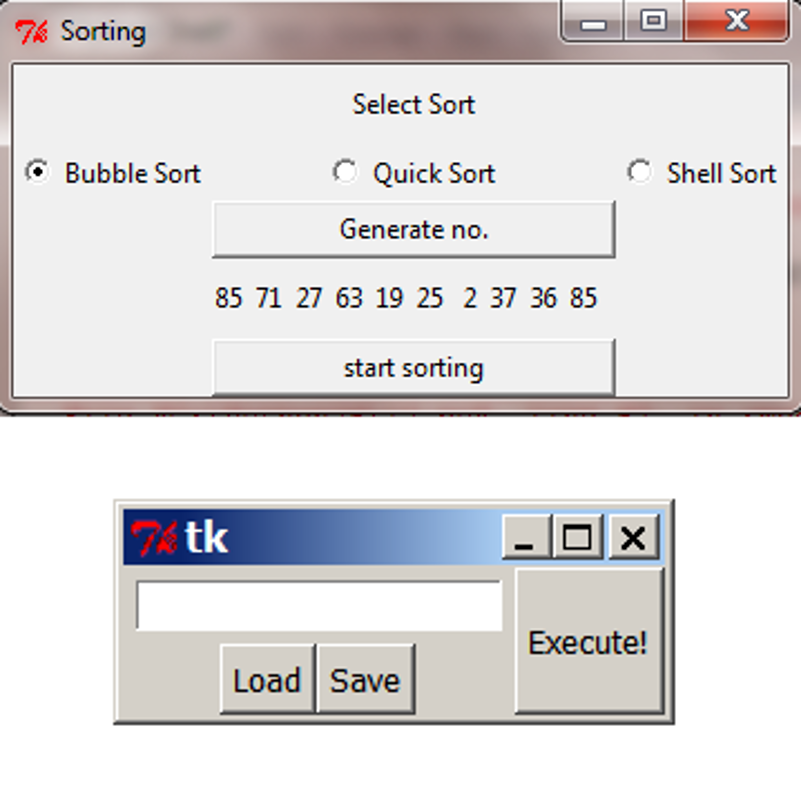
\includegraphics[width=\linewidth,keepaspectratio]{tkintergui}
\end{center}
\end{minipage}
}

\end{frame}

%%%%%%%%%%%%%%%%%%%%%%%%%%%%%%%%%%%%%%%%%%%%%%%%%%%
\begin{frame}[fragile] \frametitle{GUIs: Step by Step}
\begin{itemize}
\item Design the GUI
\item Create all the buttons, labels, entries, etc. (widgets) And specify where they go in a window
\item Write functions/methods to do what needs to be done
\item Connect the widgets to the functions/methods
\item Start the main loop
\end{itemize}
\end{frame}

%%%%%%%%%%%%%%%%%%%%%%%%%%%%%%%%%%%%%%%%%%%%%%%%%%%
\begin{frame}[fragile] \frametitle{Tkinter}
\begin{itemize}
\item Tkinter is the de facto Python standard GUI library, it comes with your installation of Python and doesn't need to be installed separately
\item We will use the Tkinter GUI toolkit to create Python GUIs \\
https://docs.python.org/3/library/tk.html 
\end{itemize}
\begin{lstlisting}
from tkinter import *
\end{lstlisting}
\end{frame}


%%%%%%%%%%%%%%%%%%%%%%%%%%%%%%%%%%%%%%%%%%%%%%%%%%%
\begin{frame}[fragile] \frametitle{Some simple tkinter widgets}

\adjustbox{valign=t}{
\begin{minipage}{0.45\linewidth}
\begin{itemize}
\item Label: Just displays text, not clickable
\item Button: Can be linked to a function/method which is called on click
\item Entry: Can allow the user to enter text, Can also be used to display text, Has 3 possible states: normal, readonly, disabled
\end{itemize}
\end{minipage}
}
\hfill
\adjustbox{valign=t}{
\begin{minipage}{0.45\linewidth}
\begin{lstlisting}
win = Tk()
win.title("My GUI")
l = Label(win, text="Hello, world")
b = Button(win, text="Click me!")
l.pack()
b.pack()

win.mainloop()
\end{lstlisting}
\begin{center}
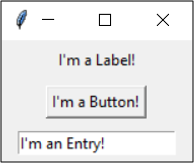
\includegraphics[width=0.5\linewidth,keepaspectratio]{tkintersimple}
\end{center}
\end{minipage}
}
This code creates a basic GUI with a Label and a Button and places them in a window using the Pack layout manager.

The button has no ``command'' so it has no function when clicked.

\end{frame}


%%%%%%%%%%%%%%%%%%%%%%%%%%%%%%%%%%%%%%%%%%%%%%%%%%%
\begin{frame}[fragile] \frametitle{Some simple tkinter widgets}

\adjustbox{valign=t}{
\begin{minipage}{0.45\linewidth}
\begin{itemize}
\item Now the clicked function will be called every time the button is clicked
\item If we defined the clicked function below the GUI code, the line creating the Button would throw a NameError
\item We can avoid this problem by writing a class for our GUI
\end{itemize}
\end{minipage}
}
\hfill
\adjustbox{valign=t}{
\begin{minipage}{0.45\linewidth}
\begin{lstlisting}
def clicked():
    print("Button clicked!")

win = Tk()
win.title("My GUI")
l = Label(win, text="Hello, world")
b = Button(win, text="Click me!", command=clicked)
l.pack()
b.pack()

win.mainloop()
\end{lstlisting}
\end{minipage}
}
\end{frame}

%%%%%%%%%%%%%%%%%%%%%%%%%%%%%%%%%%%%%%%%%%%%%%%%%%%
\begin{frame}[fragile] \frametitle{Encapsulating a GUI into an Object}

\adjustbox{valign=t}{
\begin{minipage}{0.4\linewidth}
\begin{itemize}
\item The \_\_init\_\_ method takes in a Tk window, creates GUI widgets, and packs them
\item Command is now self.clicked because clicked is a method in the class
\end{itemize}
\end{minipage}
}
\hfill
\adjustbox{valign=t}{
\begin{minipage}{0.5\linewidth}
\begin{lstlisting}
class MyGUI:

	def __init__(self, win):
		self.l = Label(win, text="Hello, world!")
		self.b = Button(win, text="Click me!", command=self.clicked)
		self.l.pack()
		self.b.pack()

	def clicked(self):
		print(``Button clicked!'')
\end{lstlisting}
\end{minipage}
}
\end{frame}

%%%%%%%%%%%%%%%%%%%%%%%%%%%%%%%%%%%%%%%%%%%%%%%%%%%
\begin{frame}[fragile] \frametitle{Encapsulating a GUI into an Object}

\adjustbox{valign=t}{
\begin{minipage}{0.45\linewidth}
\begin{itemize}
\item In the main method, we create a Tk window, give it a title, and pass it as the win argument of a new GUI object
\end{itemize}
\end{minipage}
}
\hfill
\adjustbox{valign=t}{
\begin{minipage}{0.45\linewidth}
\begin{lstlisting}
def main(args):
    win = Tk()
    win.title("My GUI")
    MyGUI(win)
    win.mainloop()

if __name__ == '__main__':
    import sys
    main(sys.argv)
\end{lstlisting}
\end{minipage}
}
\end{frame}

%%%%%%%%%%%%%%%%%%%%%%%%%%%%%%%%%%%%%%%%%%%%%%%%%%%
\begin{frame}[fragile] \frametitle{GUI layout managers}

\adjustbox{valign=t}{
\begin{minipage}{0.45\linewidth}
Pack
\begin{itemize}
\item Positions widgets relative to each other
\item Simple to use
\item Limited layout possibilities compared to grid
\end{itemize}
\end{minipage}
}
\hfill
\adjustbox{valign=t}{
\begin{minipage}{0.45\linewidth}
Grid
\begin{itemize}
\item Allows you to place widgets in rows and columns
\item More complicated than pack but good for GUIs where a particular arrangement is desired
\end{itemize}
\end{minipage}
}

Don't use grid and pack in the same container!
\end{frame}

%%%%%%%%%%%%%%%%%%%%%%%%%%%%%%%%%%%%%%%%%%%%%%%%%%%
\begin{frame}[fragile] \frametitle{Exercise: Adder}

\begin{itemize}
\item Create a GUI with two NORMAL entries and one READONLY entry
\item There should a button that, when clicked, adds the numbers entered in the first two entries and displays the sum in the third entry
\item If the calculation can't be performed due to invalid input, display a message box with an error message.

\end{itemize}

\begin{center}
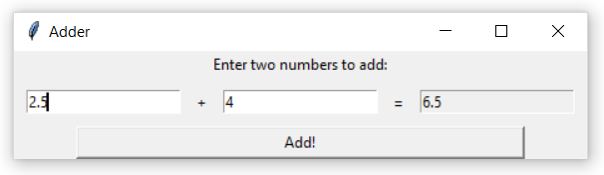
\includegraphics[width=\linewidth,keepaspectratio]{adder}
\end{center}
\end{frame}

%%%%%%%%%%%%%%%%%%%%%%%%%%%%%%%%%%%%%%%%%%%%%%%%%%%
\begin{frame}[fragile] \frametitle{Frames}

\begin{itemize}
\item Container that can be placed within a window
\item Holds other widgets
\item Each frame has its own grid layout, independent of the main window
\item You can use a different layout manager for each container
\end{itemize}
\end{frame}

%%%%%%%%%%%%%%%%%%%%%%%%%%%%%%%%%%%%%%%%%%%%%%%%%%%
\begin{frame}[fragile] \frametitle{Example: Frames (use within GUI class)}
\begin{lstlisting}
f1 = Frame(win, height=100, width=100, bd=1, relief=SUNKEN)
f2 = Frame(win, height=100, width=100, bd=1, relief=SUNKEN)

f1.grid(row=0, column=0, sticky=EW)
f2.grid(row=0, column=1, sticky=EW)

# self.l1 will be used for another method later
self.l1 = Label(f1, text="One", height=5, width=5)
self.l1.grid(row=0, column=0)
Label(f1, text="Two", height=5, width=5).grid(row=0, column=1)
Label(f2, text="Three", height=5, width=5).pack(side=LEFT)
Label(f2, text="Four", height=5, width=5).pack(side=LEFT)

\end{lstlisting}
\end{frame}

%%%%%%%%%%%%%%%%%%%%%%%%%%%%%%%%%%%%%%%%%%%%%%%%%%%
\begin{frame}[fragile] \frametitle{Radiobuttons}
\begin{itemize}
\item Allows the user to choose from one or more options
\item Can be linked to other Radiobuttons with StringVars and IntVars
\item If configured correctly, only one Radiobuttons from a group can be selected at at time
\end{itemize}
\end{frame}

%%%%%%%%%%%%%%%%%%%%%%%%%%%%%%%%%%%%%%%%%%%%%%%%%%%
\begin{frame}[fragile] \frametitle{StringVars and IntVars}
\begin{itemize}
\item Two variable classes included in Tkinter
\item Have .set() method to set their value
e.g. my\_string\_var.set(``Hello'')
\item StringVars have string value, IntVars have integer value
\item Have .get() method to get their value
e.g. val = my\_string\_var.get()
\item Can be passed in as ``variable'' argument when creating a Radiobutton, or ``textvariable'' argument when creating an Entry

\end{itemize}
\end{frame}

%%%%%%%%%%%%%%%%%%%%%%%%%%%%%%%%%%%%%%%%%%%%%%%%%%%
\begin{frame}[fragile] \frametitle{Exercise}
\begin{itemize}
\item Revisit our Adder example from the last class
\item Instead of using Entry.insert and Entry.delete, use a StringVar to change the text of the result Entry
\item See what happens if you don't set the Entry state to ``normal'' before changing the text!
\end{itemize}
\end{frame}

%%%%%%%%%%%%%%%%%%%%%%%%%%%%%%%%%%%%%%%%%%%%%%%%%%%
\begin{frame}[fragile] \frametitle{Adding Radiobuttons to our Frame example}
\begin{lstlisting}
self.color = StringVar()

rb1 = Radiobutton(win, text="Red", variable=self.color, value="red")
rb2 = Radiobutton(win, text="Blue", variable=self.color, value="blue")
rb3 = Radiobutton(win, text="Green", variable=self.color, value="green")

self.color.set("unknown") # deselects all radiobuttons linked to self.color

rb1.grid(row=1, column=0)
rb2.grid(row=2, column=0)
rb3.grid(row=3, column=0)

Button(win, text="Change Color", command=self.change_color).grid(row=1, column=1)
\end{lstlisting}
\end{frame}

%%%%%%%%%%%%%%%%%%%%%%%%%%%%%%%%%%%%%%%%%%%%%%%%%%%
\begin{frame}[fragile] \frametitle{Adding Radiobuttons to our Frame example}

\adjustbox{valign=t}{
\begin{minipage}{0.45\linewidth}
\begin{lstlisting}
def change_color(self):
	new_color = self.color.get()
	if new_color == "unknown":
		pass
       else:
       	self.l1.config(bg=new_color)
\end{lstlisting}
\end{minipage}
}
\hfill
\adjustbox{valign=t}{
\begin{minipage}{0.45\linewidth}
\begin{center}
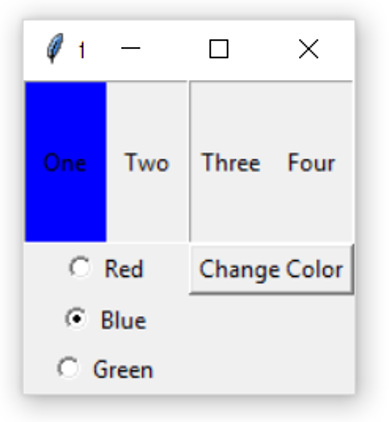
\includegraphics[width=\linewidth,keepaspectratio]{rb1}
\end{center}
\end{minipage}
}
\end{frame}

%%%%%%%%%%%%%%%%%%%%%%%%%%%%%%%%%%%%%%%%%%%%%%%%%%%
\begin{frame}[fragile] \frametitle{Additional Exercise}
\begin{itemize}
\item Add another set of Radiobuttons to the GUI. Separate from those linked to self.change\_color
\item There should be four Radiobuttons, each linked to one of the labels
\item Create an IntVar to use as the variable for these Radiobuttons
\item The user's selection should determine which Label will change color when the button is clicked.
\end{itemize}
\end{frame}

%%%%%%%%%%%%%%%%%%%%%%%%%%%%%%%%%%%%%%%%%%%%%%%%%%%
\begin{frame}[fragile] \frametitle{Root Window vs. Toplevels}
\begin{itemize}
\item The root window is your main window (Tk)
\item A GUI application should have only one root window
\item Any additional windows should be Toplevels
\item Hide windows with .withdraw()
\item Show windows with .deiconify()
\item Delete windows with .destroy() (they will be gone forever!)
\item If you destroy the root window, all Toplevels will also be destroyed

\end{itemize}
\end{frame}

%%%%%%%%%%%%%%%%%%%%%%%%%%%%%%%%%%%%%%%%%%%%%%%%%%%
\begin{frame}[fragile] \frametitle{Adding multiple windows to our example}
\begin{lstlisting}
# in __init__ method, add line: self.root = win

def new_window(self):
	self.root.withdraw()
	self.new = Toplevel()
	Label(self.new, width=30, height=10, text="I'm a new window!").pack()
	Button(self.new, text="Close window", command=self.close_new).pack()

def close_new(self):
	self.new.destroy() # destroy new window
	self.root.deiconify() # show root window

\end{lstlisting}
\end{frame}


%%%%%%%%%%%%%%%%%%%%%%%%%%%%%%%%%%%%%%%%%%%%%%%%%%%
\begin{frame}[fragile] \frametitle{Changing the GUI appearance}
\begin{itemize}
\item GUI windows and widgets have many optional parameters to change their appearance
\item bg: background color
\item fg: foreground color (for Labels, this is the font color)
\item bd: border width
\item border: border type (RAISED, SUNKEN, etc)
\item For color codes: http://htmlcolorcodes.com/ 
\item For more options, check the documentation or online tutorials
\end{itemize}
\end{frame}






%%
%%
%%%%%%%%%%%%%%%%%%%%%%%%%%%%%%%%%%%%%%%%%%%%%%%%%%%%%%%%%%%%%%%%%%%%%%%%%%%%%%%%%%%%
%%\begin{frame}[fragile]\frametitle{Graphical User Interfaces with Tkinter}
%%
%%Tk/Tcl has long been an integral part of Python.  It provides a robust
%%and platform independent windowing toolkit, that is available to
%%Python programmers using the \textbf{Tkinter} module, and its
%%extension, the \textbf{Tix} module.
%%
%%The \textbf{Tkinter} module is a thin object--oriented layer on top of
%%Tcl/Tk. To use \textbf{Tkinter}, you don't need to write Tcl code,
%%but you will need to consult the Tk documentation, and occasionally
%%the Tcl documentation.  \textbf{Tkinter} is a set of wrappers that
%%implement the Tk widgets as Python classes.  In addition, the internal
%%module \textbf{\_tkinter} provides a threadsafe mechanism which allows
%%Python and Tcl to interact.
%%
%%Tk is not the only GUI for Python, but is however the most commonly
%%used one; see section~\ref{other-gui-modules}, ``Other User Interface
%%Modules and Packages,'' for more information on other GUI toolkits for
%%Python.
%%\end{frame}
%%
%%
%%%%%%%%%%%%%%%%%%%%%%%%%%%%%%%%%%%%%%%%%%%%%%%%%%%%%%%%%%%%%%%%%%%%%%%%%%%%%%%%%%%%
%%\begin{frame}[fragile]\frametitle{Tkinter: Python interface to Tcl/Tk}
%%
%%The Tkinter module (``Tk interface'') is the standard Python
%%interface to the Tk GUI toolkit.  Both Tk and Tkinter are
%%available on most UNIX platforms, as well as on Windows and
%%Macintosh systems.  (Tk itself is not part of Python; it is maintained
%%at ActiveState.)
%%
%%\end{frame}
%%
%%
%%%%%%%%%%%%%%%%%%%%%%%%%%%%%%%%%%%%%%%%%%%%%%%%%%%%%%%%%%%%%%%%%%%%%%%%%%%%%%%%%%%%
%%\begin{frame}[fragile]\frametitle{Tkinter Modules}
%%
%%Most of the time, the \textbf{Tkinter} module is all you really
%%need, but a number of additional modules are available as well.  The
%%Tk interface is located in a binary module named \textbf{\_tkinter}.
%%This module contains the low-level interface to Tk, and should never
%%be used directly by application programmers. It is usually a shared
%%library (or DLL), but might in some cases be statically linked with
%%the Python interpreter.
%%
%%In addition to the Tk interface module, \textbf{Tkinter} includes a
%%number of Python modules. The two most important modules are the
%%\textbf{Tkinter} module itself, and a module called
%%\textbf{Tkconstants}. The former automatically imports the latter, so
%%to use Tkinter, all you need to do is to import one module:
%%
%%\begin{lstlisting}
%%import Tkinter
%%\end{lstlisting}
%%
%%Or, more often:
%%
%%\begin{lstlisting}
%%from Tkinter import *
%%\end{lstlisting}
%%
%%\end{frame}
%%
%%%%%%%%%%%%%%%%%%%%%%%%%%%%%%%%%%%%%%%%%%%%%%%%%%%%%%%%%%%%%%%%%%%%%%%%%%%%%%%%%%%%
%%\begin{frame}[fragile]\frametitle{Tkinter Modules}
%%
%%
%%The \textbf{Tk} class is instantiated without arguments.
%%This creates a toplevel widget of Tk which usually is the main window
%%of an appliation. Each instance has its own associated Tcl interpreter.
%%% FIXME: The following keyword arguments are currently recognized:
%%
%%Other modules that provide Tk support include:
%%
%%\begin{itemize}
%%% \declaremodule{standard}{Tkconstants}
%%% \modulesynopsis{Constants used by Tkinter}
%%% FIXME 
%%
%%\item[\textbf{ScrolledText}]
%%Text widget with a vertical scroll bar built in.
%%
%%\item[\textbf{tkColorChooser}]
%%Dialog to let the user choose a color.
%%
%%\item[\textbf{tkCommonDialog}]
%%Base class for the dialogs defined in the other modules listed here.
%%
%%\item[\textbf{tkFileDialog}]
%%Common dialogs to allow the user to specify a file to open or save.
%%
%%\item[\textbf{tkFont}]
%%Utilities to help work with fonts.
%%
%%\item[\textbf{tkMessageBox}]
%%Access to standard Tk dialog boxes.
%%
%%\item[\textbf{tkSimpleDialog}]
%%Basic dialogs and convenience functions.
%%
%%\item[\textbf{Tkdnd}]
%%Drag-and-drop support for \textbf{Tkinter}.
%%This is experimental and should become deprecated when it is replaced 
%%with the Tk DND.
%%
%%\item[\textbf{turtle}]
%%Turtle graphics in a Tk window.
%%
%%\end{itemize}
%%\end{frame}
%%
%%
%%%%%%%%%%%%%%%%%%%%%%%%%%%%%%%%%%%%%%%%%%%%%%%%%%%%%%%%%%%%%%%%%%%%%%%%%%%%%%%%%%%%
%%\begin{frame}[fragile]\frametitle{Tkinter Life Preserver}
%%
%%% Converted to LaTeX by Mike Clarkson.
%%
%%This section is not designed to be an exhaustive tutorial on either
%%Tk or Tkinter.  Rather, it is intended as a stop gap, providing some
%%introductory orientation on the system.
%%
%%Credits:
%%\begin{itemize}
%%\item   Tkinter was written by Steen Lumholt and Guido van Rossum.
%%\item   Tk was written by John Ousterhout while at Berkeley.
%%\item   This Life Preserver was written by Matt Conway at
%%the University of Virginia.
%%\item   The html rendering, and some liberal editing, was
%%produced from a FrameMaker version by Ken Manheimer.
%%\item   Fredrik Lundh elaborated and revised the class interface descriptions,
%%to get them current with Tk 4.2.
%%\item  Mike Clarkson converted the documentation to \LaTeX, and compiled the 
%%User Interface chapter of the reference manual.
%%\end{itemize}
%%\end{frame}
%%
%%
%%%%%%%%%%%%%%%%%%%%%%%%%%%%%%%%%%%%%%%%%%%%%%%%%%%%%%%%%%%%%%%%%%%%%%%%%%%%%%%%%%%%
%%\begin{frame}[fragile]\frametitle{How To Use This Section}
%%
%%This section is designed in two parts: the first half (roughly) covers
%%background material, while the second half can be taken to the
%%keyboard as a handy reference.
%%
%%When trying to answer questions of the form ``how do I do blah'', it
%%is often best to find out how to do``blah'' in straight Tk, and then
%%convert this back into the corresponding \textbf{Tkinter} call.
%%Python programmers can often guess at the correct Python command by
%%looking at the Tk documentation. This means that in order to use
%%Tkinter, you will have to know a little bit about Tk. This document
%%can't fulfill that role, so the best we can do is point you to the
%%best documentation that exists. Here are some hints:
%%
%%\begin{itemize}
%%\item   The authors strongly suggest getting a copy of the Tk man
%%pages. Specifically, the man pages in the \code{mann} directory are most
%%useful. The \code{man3} man pages describe the C interface to the Tk
%%library and thus are not especially helpful for script writers.  
%%
%%\item   Addison-Wesley publishes a book called \textbf{Tcl and the
%%Tk Toolkit} by John Ousterhout (ISBN 0-201-63337-X) which is a good
%%introduction to Tcl and Tk for the novice.  The book is not
%%exhaustive, and for many details it defers to the man pages. 
%%
%%\item   \textbf{Tkinter.py} is a last resort for most, but can be a good
%%place to go when nothing else makes sense.  
%%\end{itemize}
%%
%%\end{frame}
%%
%%
%%%%%%%%%%%%%%%%%%%%%%%%%%%%%%%%%%%%%%%%%%%%%%%%%%%%%%%%%%%%%%%%%%%%%%%%%%%%%%%%%%%%
%%\begin{frame}[fragile]\frametitle{A Simple Hello World Program} % HelloWorld.html
%%
%%%begin{latexonly}
%%%\begin{figure}[hbtp]
%%%\centerline{\epsfig{file=HelloWorld.gif,width=.9\textwidth}}
%%%\vspace{.5cm}
%%%\caption{HelloWorld gadget image}
%%%\end{figure}
%%%See also the hello-world \ulink{notes}{classes/HelloWorld-notes.html} and
%%%\ulink{summary}{classes/HelloWorld-summary.html}.
%%%end{latexonly}
%%
%%
%%\begin{lstlisting}
%%from Tkinter import *                                                    1
%%                                                                         2
%%class Application(Frame):                                                3
%%    def say_hi(self):                                                    4
%%        print ''hi there, everyone!''                                      5
%%                                                                         6
%%    def createWidgets(self):                                             7
%%        self.QUIT = Button(self)                                         8
%%        self.QUIT[''text''] = ''QUIT''                                       9
%%        self.QUIT[''fg'']   = ''red''                                       10
%%        self.QUIT[''command''] =  self.quit                               11
%%                                                                        12
%%        self.QUIT.pack({''side'': ''left''})                                13
%%                                                                        14
%%        self.hi_there = Button(self)                                    15
%%        self.hi_there[''text''] = ''Hello'',                                16
%%        self.hi_there[''command''] = self.say_hi                          17
%%                                                                        18
%%        self.hi_there.pack({''side'': ''left''})                            19
%%                                                                        20
%%                                                                        21
%%    def __init__(self, master=None):                                    22
%%        Frame.__init__(self, master)                                    23
%%        self.pack()                                                     24
%%        self.createWidgets()                                            25
%%                                                                        26
%%app = Application()                                                     27
%%app.mainloop()                                                          28
%%\end{lstlisting}
%%\end{frame}
%%
%%%%%%%%%%%%%%%%%%%%%%%%%%%%%%%%%%%%%%%%%%%%%%%%%%%%%%%%%%%%%%%%%%%%%%%%%%%%%%%%%%%%
%%\begin{frame}[fragile]\frametitle{A (Very) Quick Look at Tcl/Tk} % BriefTclTk.html
%%
%%The class hierarchy looks complicated, but in actual practice,
%%application programmers almost always refer to the classes at the very
%%bottom of the hierarchy. 
%%
%%Notes:
%%\begin{itemize}
%%\item   These classes are provided for the purposes of
%%organizing certain functions under one namespace. They aren't meant to
%%be instantiated independently.
%%
%%\item    The \textbf{Tk} class is meant to be instantiated only once in
%%an application. Application programmers need not instantiate one
%%explicitly, the system creates one whenever any of the other classes
%%are instantiated.
%%
%%\item    The \textbf{Widget} class is not meant to be instantiated, it
%%is meant only for subclassing to make ``real'' widgets (in Cpp, this
%%is called an `abstract class').
%%\end{itemize}
%%
%%To make use of this reference material, there will be times when you
%%will need to know how to read short passages of Tk and how to identify
%%the various parts of a Tk command.  
%%(See section~\ref{tkinter-basic-mapping} for the
%%\textbf{Tkinter} equivalents of what's below.)
%%
%%\end{frame}
%%
%%%%%%%%%%%%%%%%%%%%%%%%%%%%%%%%%%%%%%%%%%%%%%%%%%%%%%%%%%%%%%%%%%%%%%%%%%%%%%%%%%%%
%%\begin{frame}[fragile]\frametitle{A (Very) Quick Look at Tcl/Tk} % BriefTclTk.html
%%
%%Tk scripts are Tcl programs.  Like all Tcl programs, Tk scripts are
%%just lists of tokens separated by spaces.  A Tk widget is just its
%%\emph{class}, the \emph{options} that help configure it, and the
%%\emph{actions} that make it do useful things. 
%%
%%To make a widget in Tk, the command is always of the form: 
%%
%%\begin{lstlisting}
%%                classCommand newPathname options
%%\end{lstlisting}
%%
%%\begin{itemize}
%%\item[\textbf{classCommand}]
%%denotes which kind of widget to make (a button, a label, a menu...)
%%
%%\item[\textbf{newPathname}]
%%is the new name for this widget.  All names in Tk must be unique.  To
%%help enforce this, widgets in Tk are named with \emph{pathnames}, just
%%like files in a file system.  The top level widget, the \emph{root},
%%is called \code{.} (period) and children are delimited by more
%%periods.  For example, \code{.myApp.controlPanel.okButton} might be
%%the name of a widget.
%%
%%\item[\textbf{options} ]
%%configure the widget's appearance and in some cases, its
%%behavior.  The options come in the form of a list of flags and values.
%%Flags are proceeded by a `-', like unix shell command flags, and
%%values are put in quotes if they are more than one word.
%%\end{itemize}
%%
%%\end{frame}
%%
%%%%%%%%%%%%%%%%%%%%%%%%%%%%%%%%%%%%%%%%%%%%%%%%%%%%%%%%%%%%%%%%%%%%%%%%%%%%%%%%%%%%
%%\begin{frame}[fragile]\frametitle{A (Very) Quick Look at Tcl/Tk} % BriefTclTk.html
%%
%%For example: 
%%
%%\begin{lstlisting}
%%    button   .fred   -fg red -text ''hi there''
%%       ^       ^     \_____________________/
%%       |       |                |
%%     class    new            options
%%    command  widget  (-opt val -opt val ...)
%%\end{lstlisting} 
%%
%%Once created, the pathname to the widget becomes a new command.  This
%%new \textbf{widget command} is the programmer's handle for getting the new
%%widget to perform some \textbf{action}.  In C, you'd express this as
%%someAction(fred, someOptions), in Cpp, you would express this as
%%fred.someAction(someOptions), and in Tk, you say: 
%%
%%\begin{lstlisting}
%%    .fred someAction someOptions 
%%\end{lstlisting} 
%%
%%Note that the object name, \code{.fred}, starts with a dot.
%%
%%As you'd expect, the legal values for \textbf{someAction} will depend on
%%the widget's class: \code{.fred disable} works if fred is a
%%button (fred gets greyed out), but does not work if fred is a label
%%(disabling of labels is not supported in Tk). 
%%
%%The legal values of \textbf{someOptions} is action dependent.  Some
%%actions, like \code{disable}, require no arguments, others, like
%%a text-entry box's \code{delete} command, would need arguments
%%to specify what range of text to delete.  
%%\end{frame}
%%
%%
%%%%%%%%%%%%%%%%%%%%%%%%%%%%%%%%%%%%%%%%%%%%%%%%%%%%%%%%%%%%%%%%%%%%%%%%%%%%%%%%%%%%
%%\begin{frame}[fragile]\frametitle{Mapping Basic Tk into Tkinter} % BriefTclTk.html
%%
%%
%%Class commands in Tk correspond to class constructors in Tkinter.
%%
%%\begin{lstlisting}
%%    button .fred                =====>  fred = Button()
%%\end{lstlisting}
%%
%%The master of an object is implicit in the new name given to it at
%%creation time.  In Tkinter, masters are specified explicitly.
%%
%%\begin{lstlisting}
%%    button .panel.fred          =====>  fred = Button(panel)
%%\end{lstlisting}
%%
%%The configuration options in Tk are given in lists of hyphened tags
%%followed by values.  In Tkinter, options are specified as
%%keyword-arguments in the instance constructor, and keyword-args for
%%configure calls or as instance indices, in dictionary style, for
%%established instances.  See section~\ref{tkinter-setting-options} on
%%setting options.
%%
%%\begin{lstlisting}
%%    button .fred -fg red        =====>  fred = Button(panel, fg = ''red'')
%%    .fred configure -fg red     =====>  fred[''fg''] = red
%%                                OR ==>  fred.config(fg = ''red'')
%%\end{lstlisting}
%%
%%\end{frame}
%%
%%%%%%%%%%%%%%%%%%%%%%%%%%%%%%%%%%%%%%%%%%%%%%%%%%%%%%%%%%%%%%%%%%%%%%%%%%%%%%%%%%%%
%%\begin{frame}[fragile]\frametitle{} % BriefTclTk.html
%%In Tk, to perform an action on a widget, use the widget name as a
%%command, and follow it with an action name, possibly with arguments
%%(options).  In Tkinter, you call methods on the class instance to
%%invoke actions on the widget.  The actions (methods) that a given
%%widget can perform are listed in the Tkinter.py module.
%%
%%\begin{lstlisting}
%%    .fred invoke                =====>  fred.invoke()
%%\end{lstlisting}
%%
%%To give a widget to the packer (geometry manager), you call pack with
%%optional arguments.  In Tkinter, the Pack class holds all this
%%functionality, and the various forms of the pack command are
%%implemented as methods.  All widgets in \textbf{Tkinter} are
%%subclassed from the Packer, and so inherit all the packing
%%methods. See the \textbf{Tix} module documentation for additional
%%information on the Form geometry manager.
%%
%%\begin{lstlisting}
%%    pack .fred -side left       =====>  fred.pack(side = ''left'')
%%\end{lstlisting}
%%\end{frame}
%%
%%
%%%%%%%%%%%%%%%%%%%%%%%%%%%%%%%%%%%%%%%%%%%%%%%%%%%%%%%%%%%%%%%%%%%%%%%%%%%%%%%%%%%%
%%\begin{frame}[fragile]\frametitle{How Tk and Tkinter are Related} % Relationship.html
%%
%%\note{This was derived from a graphical image; the image will be used
%%      more directly in a subsequent version of this document.}
%%
%%From the top down:
%%\begin{itemize}
%%\item[\textbf{Your App Here (Python)}]
%%A Python application makes a \textbf{Tkinter} call.
%%
%%\item[\textbf{Tkinter (Python Module)}]
%%This call (say, for example, creating a button widget), is
%%implemented in the \emph{Tkinter} module, which is written in
%%Python.  This Python function will parse the commands and the
%%arguments and convert them into a form that makes them look as if they
%%had come from a Tk script instead of a Python script.
%%
%%\item[\textbf{tkinter (C)}]
%%These commands and their arguments will be passed to a C function
%%in the \emph{tkinter} - note the lowercase - extension module.
%%
%%\item[\textbf{Tk Widgets} (C and Tcl)]
%%This C function is able to make calls into other C modules,
%%including the C functions that make up the Tk library.  Tk is
%%implemented in C and some Tcl.  The Tcl part of the Tk widgets is used
%%to bind certain default behaviors to widgets, and is executed once at
%%the point where the Python \textbf{Tkinter} module is
%%imported. (The user never sees this stage).
%%
%%\item[\textbf{Tk (C)}]
%%The Tk part of the Tk Widgets implement the final mapping to ...
%%
%%\item[\textbf{Xlib (C)}]
%%the Xlib library to draw graphics on the screen.
%%\end{itemize}
%%
%%\end{frame}
%%
%%
%%%%%%%%%%%%%%%%%%%%%%%%%%%%%%%%%%%%%%%%%%%%%%%%%%%%%%%%%%%%%%%%%%%%%%%%%%%%%%%%%%%%
%%\begin{frame}[fragile]\frametitle{Setting Options -tkinter-setting-options}
%%
%%Options control things like the color and border width of a widget.
%%Options can be set in three ways:
%%
%%\begin{itemize}
%%\item[At object creation time, using keyword arguments]:
%%\begin{lstlisting}
%%fred = Button(self, fg = ''red'', bg = ''blue'')
%%\end{lstlisting}
%%\item[After object creation, treating the option name like a dictionary index]:
%%\begin{lstlisting}
%%fred[''fg''] = ''red''
%%fred[''bg''] = ''blue''
%%\end{lstlisting}
%%\item[Use the config() method to update multiple attrs subesequent to
%%object creation]:
%%\begin{lstlisting}
%%fred.config(fg = ''red'', bg = ''blue'')
%%\end{lstlisting}
%%\end{itemize}
%%
%%\end{frame}
%%
%%%%%%%%%%%%%%%%%%%%%%%%%%%%%%%%%%%%%%%%%%%%%%%%%%%%%%%%%%%%%%%%%%%%%%%%%%%%%%%%%%%%
%%\begin{frame}[fragile]\frametitle{Setting Options -tkinter-setting-options}
%%
%%For a complete explanation of a given option and its behavior, see the
%%Tk man pages for the widget in question.
%%
%%Note that the man pages list ''STANDARD OPTIONS'' and ''WIDGET SPECIFIC
%%OPTIONS'' for each widget.  The former is a list of options that are
%%common to many widgets, the latter are the options that are
%%ideosyncratic to that particular widget. 
%%No distinction between standard and widget-specific options is made in
%%this document.  Some options don't apply to some kinds of widgets.
%%Whether a given widget responds to a particular option depends on the
%%class of the widget; buttons have a \code{command} option, labels do not. 
%%
%%The options supported by a given widget are listed in that widget's
%%man page, or can be queried at runtime by calling the
%%\textbf{config()} method without arguments, or by calling the
%%\textbf{keys()} method on that widget.  The return value of these
%%calls is a dictionary whose key is the name of the option as a string
%%(for example, \code{'relief'}) and whose values are 5-tuples.
%%
%%\end{frame}
%%
%%%%%%%%%%%%%%%%%%%%%%%%%%%%%%%%%%%%%%%%%%%%%%%%%%%%%%%%%%%%%%%%%%%%%%%%%%%%%%%%%%%%
%%\begin{frame}[fragile]\frametitle{Setting Options -tkinter-setting-options}
%%Some options, like \code{bg} are synonyms for common options with long
%%names (\code{bg} is shorthand for ''background''). Passing the
%%\code{config()} method the name of a shorthand option will return a
%%2-tuple, not 5-tuple. The 2-tuple passed back will contain the name of
%%the synonym and the ``real'' option (such as \code{('bg',
%%'background')}).
%%
%%%\begin{table}{c|l|l}{textrm}{Index}{Meaning}{Example}
%%%  \lineiii{0}{option name}                       {\code{'relief'}}
%%%  \lineiii{1}{option name for database lookup}   {\code{'relief'}}
%%%  \lineiii{2}{option class for database lookup}  {\code{'Relief'}}
%%%  \lineiii{3}{default value}                     {\code{'raised'}}
%%%  \lineiii{4}{current value}                     {\code{'groove'}}
%%%\end{table}
%%
%%
%%Example:
%%
%%\begin{lstlisting}
%%>>> print fred.config()
%%{'relief' : ('relief', 'relief', 'Relief', 'raised', 'groove')}
%%\end{lstlisting}
%%
%%Of course, the dictionary printed will include all the options
%%available and their values.  This is meant only as an example.
%%
%%\end{frame}
%%
%%
%%
%%%%%%%%%%%%%%%%%%%%%%%%%%%%%%%%%%%%%%%%%%%%%%%%%%%%%%%%%%%%%%%%%%%%%%%%%%%%%%%%%%%%
%%\begin{frame}[fragile]\frametitle{The Packer} % Packer.html
%%
%%
%%The packer is one of Tk's geometry-management mechanisms.  See also
%%\textbf[classes/ClassPacker.html]{the Packer class interface}.
%%
%%Geometry managers are used to specify the relative positioning of the
%%positioning of widgets within their container - their mutual
%%\emph{master}.  In contrast to the more cumbersome \emph{placer}
%%(which is used less commonly, and we do not cover here), the packer
%%takes qualitative relationship specification - \emph{above}, \emph{to
%%the left of}, \emph{filling}, etc - and works everything out to
%%determine the exact placement coordinates for you. 
%%
%%The size of any \emph{master} widget is determined by the size of
%%the ''slave widgets'' inside.  The packer is used to control where slave
%%widgets appear inside the master into which they are packed.  You can
%%pack widgets into frames, and frames into other frames, in order to
%%achieve the kind of layout you desire.  Additionally, the arrangement
%%is dynamically adjusted to accomodate incremental changes to the
%%configuration, once it is packed.
%%
%%Note that widgets do not appear until they have had their geometry
%%specified with a geometry manager.  It's a common early mistake to
%%leave out the geometry specification, and then be surprised when the
%%widget is created but nothing appears.  A widget will appear only
%%after it has had, for example, the packer's \textbf{pack()} method
%%applied to it.
%%
%%The pack() method can be called with keyword-option/value pairs that
%%control where the widget is to appear within its container, and how it
%%is to behave when the main application window is resized.  Here are
%%some examples:
%%
%%\begin{lstlisting}
%%    fred.pack()                     # defaults to side = ''top''
%%    fred.pack(side = ''left'')
%%    fred.pack(expand = 1)
%%\end{lstlisting}
%%
%%\end{frame}
%%
%%
%%%%%%%%%%%%%%%%%%%%%%%%%%%%%%%%%%%%%%%%%%%%%%%%%%%%%%%%%%%%%%%%%%%%%%%%%%%%%%%%%%%%
%%\begin{frame}[fragile]\frametitle{Packer Options}
%%
%%For more extensive information on the packer and the options that it
%%can take, see the man pages and page 183 of John Ousterhout's book.
%%
%%\begin{itemize}
%%\item[\textbf{anchor }]
%%Anchor type.  Denotes where the packer is to place each slave in its
%%parcel.
%%
%%\item[\textbf{expand}]
%%Boolean, \code{0} or \code{1}.
%%
%%\item[\textbf{fill}]
%%Legal values: \code{'x'}, \code{'y'}, \code{'both'}, \code{'none'}.
%%
%%\item[\textbf{ipadx} and \textbf{ipady}]
%%A distance - designating internal padding on each side of the slave
%%widget.
%%
%%\item[\textbf{padx} and \textbf{pady}]
%%A distance - designating external padding on each side of the slave
%%widget.
%%
%%\item[\textbf{side}]
%%Legal values are: \code{'left'}, \code{'right'}, \code{'top'},
%%\code{'bottom'}.
%%\end{itemize}
%%
%%\end{frame}
%%

%%\subsubsection{Coupling Widget Variables} % VarCouplings.html
%%
%%The current-value setting of some widgets (like text entry widgets)
%%can be connected directly to application variables by using special
%%options.  These options are \code{variable}, \code{textvariable},
%%\code{onvalue}, \code{offvalue}, and \code{value}.  This
%%connection works both ways: if the variable changes for any reason,
%%the widget it's connected to will be updated to reflect the new value. 
%%
%%Unfortunately, in the current implementation of \textbf{Tkinter} it is
%%not possible to hand over an arbitrary Python variable to a widget
%%through a \code{variable} or \code{textvariable} option.  The only
%%kinds of variables for which this works are variables that are
%%subclassed from a class called Variable, defined in the
%%\textbf{Tkinter} module.
%%
%%There are many useful subclasses of Variable already defined:
%%\textbf{StringVar}, \textbf{IntVar}, \textbf{DoubleVar}, and
%%\textbf{BooleanVar}.  To read the current value of such a variable,
%%call the \textbf{get()} method on
%%it, and to change its value you call the \textbf{set()} method.  If
%%you follow this protocol, the widget will always track the value of
%%the variable, with no further intervention on your part.
%%
%%For example: 
%%\begin{lstlisting}
%%class App(Frame):
%%    def __init__(self, master=None):
%%        Frame.__init__(self, master)
%%        self.pack()
%%        
%%        self.entrythingy = Entry()
%%        self.entrythingy.pack()
%%        
%%        self.button.pack()
%%        # here is the application variable
%%        self.contents = StringVar()
%%        # set it to some value
%%        self.contents.set(''this is a variable'')
%%        # tell the entry widget to watch this variable
%%        self.entrythingy[''textvariable''] = self.contents
%%        
%%        # and here we get a callback when the user hits return.
%%        # we will have the program print out the value of the
%%        # application variable when the user hits return
%%        self.entrythingy.bind('<Key-Return>',
%%                              self.print_contents)
%%
%%    def print_contents(self, event):
%%        print ''hi. contents of entry is now ---->'', \
%%              self.contents.get()
%%\end{lstlisting}
%%
%%
%%\subsubsection{The Window Manager} % WindowMgr.html
%%\index{window manager (widgets)}
%%
%%In Tk, there is a utility command, \code{wm}, for interacting with the
%%window manager.  Options to the \code{wm} command allow you to control
%%things like titles, placement, icon bitmaps, and the like.  In
%%\textbf{Tkinter}, these commands have been implemented as methods
%%on the \textbf{Wm} class.  Toplevel widgets are subclassed from the
%%\textbf{Wm} class, and so can call the \textbf{Wm} methods directly.
%%
%%%See also \textbf[classes/ClassWm.html]{the Wm class interface}.
%%
%%To get at the toplevel window that contains a given widget, you can
%%often just refer to the widget's master.  Of course if the widget has
%%been packed inside of a frame, the master won't represent a toplevel
%%window.  To get at the toplevel window that contains an arbitrary
%%widget, you can call the \textbf{_root()} method.  This
%%method begins with an underscore to denote the fact that this function
%%is part of the implementation, and not an interface to Tk functionality.
%%
%%Here are some examples of typical usage:
%%
%%\begin{lstlisting}
%%import Tkinter
%%class App(Frame):
%%    def __init__(self, master=None):
%%        Frame.__init__(self, master)
%%        self.pack()
%%
%%
%%# create the application
%%myapp = App()
%%
%%#
%%# here are method calls to the window manager class
%%#
%%myapp.master.title(''My Do-Nothing Application'')
%%myapp.master.maxsize(1000, 400)
%%
%%# start the program
%%myapp.mainloop()
%%\end{lstlisting}
%%
%%
%%\subsubsection{Tk Option Data Types} % OptionTypes.html
%%
%%\index{Tk Option Data Types}
%%
%%\begin{itemize}
%%\item[anchor]
%%Legal values are points of the compass: \code{''n''},
%%\code{''ne''}, \code{''e''}, \code{''se''}, \code{''s''},
%%\code{''sw''}, \code{''w''}, \code{''nw''}, and also
%%\code{''center''}.
%%
%%\item[bitmap]
%%There are eight built-in, named bitmaps: \code{'error'}, \code{'gray25'},
%%\code{'gray50'}, \code{'hourglass'}, \code{'info'}, \code{'questhead'},
%%\code{'question'}, \code{'warning'}.  To specify an X bitmap
%%filename, give the full path to the file, preceded with an \code{@},
%%as in \code{''@/usr/contrib/bitmap/gumby.bit''}.
%%
%%\item[boolean]
%%You can pass integers 0 or 1 or the stings \code{''yes''} or \code{''no''} .
%%
%%\item[callback]
%%This is any Python function that takes no arguments.  For example: 
%%\begin{lstlisting}
%%    def print_it():
%%            print ''hi there''
%%    fred[''command''] = print_it
%%\end{lstlisting}
%%
%%\item[color]
%%Colors can be given as the names of X colors in the rgb.txt file,
%%or as strings representing RGB values in 4 bit: \code{''\#RGB''}, 8
%%bit: \code{''\#RRGGBB''}, 12 bit'' \code{''\#RRRGGGBBB''}, or 16 bit
%%\code{''\#RRRRGGGGBBBB''} ranges, where R,G,B here represent any
%%legal hex digit.  See page 160 of Ousterhout's book for details.  
%%
%%\item[cursor]
%%The standard X cursor names from \textbf{cursorfont.h} can be used,
%%without the \code{XC_} prefix.  For example to get a hand cursor
%%(\constant{XC_hand2}), use the string \code{''hand2''}.  You can also
%%specify a bitmap and mask file of your own.  See page 179 of
%%Ousterhout's book.
%%
%%\item[distance]
%%Screen distances can be specified in either pixels or absolute
%%distances.  Pixels are given as numbers and absolute distances as
%%strings, with the trailing character denoting units: \code{c}
%%for centimeters, \code{i} for inches, \code{m} for millimeters,
%%\code{p} for printer's points.  For example, 3.5 inches is expressed
%%as \code{''3.5i''}.
%%
%%\item[font]
%%Tk uses a list font name format, such as \code{\{courier 10 bold\}}.
%%Font sizes with positive numbers are measured in points;
%%sizes with negative numbers are measured in pixels.
%%
%%\item[geometry]
%%This is a string of the form \samp{\textbf{width}x\textbf{height}}, where
%%width and height are measured in pixels for most widgets (in
%%characters for widgets displaying text).  For example:
%%\code{fred[''geometry''] = ''200x100''}.
%%
%%\item[justify]
%%Legal values are the strings: \code{''left''},
%%\code{''center''}, \code{''right''}, and \code{''fill''}.
%%
%%\item[region]
%%This is a string with four space-delimited elements, each of
%%which is a legal distance (see above).  For example: \code{''2 3 4
%%5''} and \code{''3i 2i 4.5i 2i''} and \code{''3c 2c 4c 10.43c''} 
%%are all legal regions.
%%
%%\item[relief]
%%Determines what the border style of a widget will be.  Legal
%%values are: \code{''raised''}, \code{''sunken''},
%%\code{''flat''}, \code{''groove''}, and \code{''ridge''}.
%%
%%\item[scrollcommand]
%%This is almost always the \textbf{set()} method of some scrollbar
%%widget, but can be any widget method that takes a single argument.  
%%Refer to the file \textbf{Demo/tkinter/matt/canvas-with-scrollbars.py}
%%in the Python source distribution for an example.
%%
%%\item[wrap:]
%%Must be one of: \code{''none''}, \code{''char''}, or \code{''word''}.
%%\end{itemize}
%%
%%
%%\subsubsection{Bindings and Events} % Bindings.html
%%
%%\index{bind (widgets)}
%%\index{events (widgets)}
%%
%%The bind method from the widget command allows you to watch for
%%certain events and to have a callback function trigger when that event
%%type occurs.  The form of the bind method is:
%%
%%\begin{lstlisting}
%%    def bind(self, sequence, func, add=''):
%%\end{lstlisting}
%%where:
%%
%%\begin{itemize}
%%\item[sequence]
%%is a string that denotes the target kind of event.  (See the bind
%%man page and page 201 of John Ousterhout's book for details).
%%
%%\item[func]
%%is a Python function, taking one argument, to be invoked when the
%%event occurs.  An Event instance will be passed as the argument.
%%(Functions deployed this way are commonly known as \textbf{callbacks}.)
%%
%%\item[add]
%%is optional, either \samp{} or \samp{+}.  Passing an empty string
%%denotes that this binding is to replace any other bindings that this
%%event is associated with.  Preceeding with a \samp{+} means that this
%%function is to be added to the list of functions bound to this event type.
%%\end{itemize}
%%
%%For example:
%%\begin{lstlisting}
%%    def turnRed(self, event):
%%        event.widget[''activeforeground''] = ''red''
%%
%%    self.button.bind(''<Enter>'', self.turnRed)
%%\end{lstlisting}
%%
%%Notice how the widget field of the event is being accesed in the
%%\textbf{turnRed()} callback.  This field contains the widget that
%%caught the X event.  The following table lists the other event fields
%%you can access, and how they are denoted in Tk, which can be useful
%%when referring to the Tk man pages.
%%
%%\begin{lstlisting}
%%Tk      Tkinter Event Field             Tk      Tkinter Event Field 
%%--      -------------------             --      -------------------
%%%f      focus                           %A      char
%%%h      height                          %E      send_event
%%%k      keycode                         %K      keysym
%%%s      state                           %N      keysym_num
%%%t      time                            %T      type
%%%w      width                           %W      widget
%%%x      x                               %X      x_root
%%%y      y                               %Y      y_root
%%\end{lstlisting}
%%
%%
%%\subsubsection{The index Parameter} % Index.html
%%
%%A number of widgets require``index'' parameters to be passed.  These
%%are used to point at a specific place in a Text widget, or to
%%particular characters in an Entry widget, or to particular menu items
%%in a Menu widget.
%%
%%\begin{itemize}
%%\item[\textbf{Entry widget indexes (index, view index, etc.)}]
%%Entry widgets have options that refer to character positions in the
%%text being displayed.  You can use these \textbf{Tkinter} functions
%%to access these special points in text widgets:
%%
%%\begin{itemize}
%%\item[AtEnd()]
%%refers to the last position in the text
%%
%%\item[AtInsert()]
%%refers to the point where the text cursor is
%%
%%\item[AtSelFirst()]
%%indicates the beginning point of the selected text
%%
%%\item[AtSelLast()]
%%denotes the last point of the selected text and finally
%%
%%\item[At(x\optional{, y})]
%%refers to the character at pixel location \textbf{x}, \textbf{y} (with
%%\textbf{y} not used in the case of a text entry widget, which contains a
%%single line of text).
%%\end{itemize}
%%
%%\item[\textbf{Text widget indexes}]
%%The index notation for Text widgets is very rich and is best described
%%in the Tk man pages.
%%
%%\item[\textbf{Menu indexes (menu.invoke(), menu.entryconfig(), etc.)}]
%%
%%Some options and methods for menus manipulate specific menu entries.
%%Anytime a menu index is needed for an option or a parameter, you may
%%pass in: 
%%\begin{itemize}
%%\item   an integer which refers to the numeric position of the entry in
%%the widget, counted from the top, starting with 0; 
%%\item   the string \code{'active'}, which refers to the menu position that is
%%currently under the cursor;
%%\item   the string \code{''last''} which refers to the last menu
%%item;  
%%\item   An integer preceded by \code{@}, as in \code{@6}, where the integer is
%%interpreted as a y pixel coordinate in the menu's coordinate system;
%%\item   the string \code{''none''}, which indicates no menu entry at all, most
%%often used with menu.activate() to deactivate all entries, and
%%finally,
%%\item   a text string that is pattern matched against the label of the
%%menu entry, as scanned from the top of the menu to the bottom.  Note
%%that this index type is considered after all the others, which means
%%that matches for menu items labelled \code{last}, \code{active}, or
%%\code{none} may be interpreted as the above literals, instead.
%%\end{itemize}
%%\end{itemize}
%%
%%
%%\section{\textbf{Tix} ---
%%         Extension widgets for Tk}
%%
%%\declaremodule{standard}{Tix}
%%\modulesynopsis{Tk Extension Widgets for Tkinter}
%%\sectionauthor{Mike Clarkson}{mikeclarkson@users.sourceforge.net}
%%
%%\index{Tix}
%%
%%The \textbf{Tix} (Tk Interface Extension) module provides an
%%additional rich set of widgets. Although the standard Tk library has
%%many useful widgets, they are far from complete. The \textbf{Tix}
%%library provides most of the commonly needed widgets that are missing
%%from standard Tk: \textbf{HList}, \textbf{ComboBox}, \textbf{Control}
%%(a.k.a. SpinBox) and an assortment of scrollable widgets. \textbf{Tix}
%%also includes many more widgets that are generally useful in a wide
%%range of applications: \textbf{NoteBook}, \textbf{FileEntry},
%%\textbf{PanedWindow}, etc; there are more than 40 of them.
%%
%%With all these new widgets, you can introduce new interaction
%%techniques into applications, creating more useful and more intuitive
%%user interfaces. You can design your application by choosing the most
%%appropriate widgets to match the special needs of your application and
%%users. 
%%
%%\begin{seealso}
%%\seetitle[http://tix.sourceforge.net/]
%%        {Tix Homepage}
%%        {The home page for \textbf{Tix}.  This includes links to
%%         additional documentation and downloads.}
%%\seetitle[http://tix.sourceforge.net/dist/current/man/]
%%        {Tix Man Pages}
%%        {On-line version of the man pages and reference material.}
%%\seetitle[http://tix.sourceforge.net/dist/current/docs/tix-book/tix.book.html]
%%        {Tix Programming Guide}
%%        {On-line version of the programmer's reference material.}
%%\seetitle[http://tix.sourceforge.net/Tide/]
%%        {Tix Development Applications}
%%        {Tix applications for development of Tix and Tkinter programs.
%%         Tide applications work under Tk or Tkinter, and include
%%         \program{TixInspect}, an inspector to remotely modify and
%%         debug Tix/Tk/Tkinter applications.}
%%\end{seealso}
%%
%%
%%\subsection{Using Tix}
%%
%%\begin{classdesc}{Tix}{screenName\optional{, baseName\optional{, className}}}
%%    Toplevel widget of Tix which represents mostly the main window
%%    of an application. It has an associated Tcl interpreter.
%%
%%Classes in the \textbf{Tix} module subclasses the classes in the
%%\textbf{Tkinter} module. The former imports the latter, so to use
%%\textbf{Tix} with Tkinter, all you need to do is to import one
%%module. In general, you can just import \textbf{Tix}, and replace
%%the toplevel call to \textbf{Tkinter.Tk} with \textbf{Tix.Tk}:
%%\begin{lstlisting}
%%import Tix
%%from Tkconstants import *
%%root = Tix.Tk()
%%\end{lstlisting}
%%\end{classdesc}
%%
%%To use \textbf{Tix}, you must have the \textbf{Tix} widgets installed,
%%usually alongside your installation of the Tk widgets.
%%To test your installation, try the following:
%%\begin{lstlisting}
%%import Tix
%%root = Tix.Tk()
%%root.tk.eval('package require Tix')
%%\end{lstlisting}
%%
%%If this fails, you have a Tk installation problem which must be
%%resolved before proceeding. Use the environment variable \envvar{TIX_LIBRARY}
%%to point to the installed \textbf{Tix} library directory, and
%%make sure you have the dynamic object library (\textbf{tix8183.dll} or
%%\textbf{libtix8183.so}) in  the same directory that contains your Tk
%%dynamic object library (\textbf{tk8183.dll} or \textbf{libtk8183.so}). The
%%directory with the dynamic object library should also have a file
%%called \textbf{pkgIndex.tcl} (case sensitive), which contains the line:
%%
%%\begin{lstlisting}
%%package ifneeded Tix 8.1 [list load ''[file join $dir tix8183.dll]'' Tix]
%%\end{lstlisting} % $ <-- bow to font-lock
%%
%%
%%\subsection{Tix Widgets}
%%
%%\ulink{Tix}
%%{http://tix.sourceforge.net/dist/current/man/html/TixCmd/TixIntro.htm}
%%introduces over 40 widget classes to the \textbf{Tkinter} 
%%repertoire.  There is a demo of all the \textbf{Tix} widgets in the
%%\textbf{Demo/tix} directory of the standard distribution.
%%
%%
%%% The Python sample code is still being added to Python, hence commented out
%%
%%
%%\subsubsection{Basic Widgets}
%%
%%\begin{classdesc}{Balloon}{}
%%A \ulink{Balloon}
%%{http://tix.sourceforge.net/dist/current/man/html/TixCmd/tixBalloon.htm}
%%that pops up over a widget to provide help.  When the user moves the
%%cursor inside a widget to which a Balloon widget has been bound, a
%%small pop-up window with a descriptive message will be shown on the
%%screen.
%%\end{classdesc}
%%
%%% Python Demo of:
%%% \ulink{Balloon}{http://tix.sourceforge.net/dist/current/demos/samples/Balloon.tcl}
%%
%%\begin{classdesc}{ButtonBox}{}
%%The \ulink{ButtonBox}
%%{http://tix.sourceforge.net/dist/current/man/html/TixCmd/tixButtonBox.htm}
%%widget creates a box of buttons, such as is commonly used for \code{Ok
%%Cancel}.
%%\end{classdesc}
%%
%%% Python Demo of:
%%% \ulink{ButtonBox}{http://tix.sourceforge.net/dist/current/demos/samples/BtnBox.tcl}
%%
%%\begin{classdesc}{ComboBox}{}
%%The \ulink{ComboBox}
%%{http://tix.sourceforge.net/dist/current/man/html/TixCmd/tixComboBox.htm}
%%widget is similar to the combo box control in MS Windows. The user can
%%select a choice by either typing in the entry subwdget or selecting
%%from the listbox subwidget.
%%\end{classdesc}
%%
%%% Python Demo of:
%%% \ulink{ComboBox}{http://tix.sourceforge.net/dist/current/demos/samples/ComboBox.tcl}
%%
%%\begin{classdesc}{Control}{}
%%The \ulink{Control}
%%{http://tix.sourceforge.net/dist/current/man/html/TixCmd/tixControl.htm}
%%widget is also known as the \textbf{SpinBox} widget. The user can
%%adjust the value by pressing the two arrow buttons or by entering the
%%value directly into the entry. The new value will be checked against
%%the user-defined upper and lower limits.
%%\end{classdesc}
%%
%%% Python Demo of:
%%% \ulink{Control}{http://tix.sourceforge.net/dist/current/demos/samples/Control.tcl}
%%
%%\begin{classdesc}{LabelEntry}{}
%%The \ulink{LabelEntry}
%%{http://tix.sourceforge.net/dist/current/man/html/TixCmd/tixLabelEntry.htm}
%%widget packages an entry widget and a label into one mega widget. It
%%can be used be used to simplify the creation of ``entry-form'' type of
%%interface.
%%\end{classdesc}
%%
%%% Python Demo of:
%%% \ulink{LabelEntry}{http://tix.sourceforge.net/dist/current/demos/samples/LabEntry.tcl}
%%
%%\begin{classdesc}{LabelFrame}{}
%%The \ulink{LabelFrame}
%%{http://tix.sourceforge.net/dist/current/man/html/TixCmd/tixLabelFrame.htm}
%%widget packages a frame widget and a label into one mega widget.  To
%%create widgets inside a LabelFrame widget, one creates the new widgets
%%relative to the \member{frame} subwidget and manage them inside the
%%\member{frame} subwidget.
%%\end{classdesc}
%%
%%% Python Demo of:
%%% \ulink{LabelFrame}{http://tix.sourceforge.net/dist/current/demos/samples/LabFrame.tcl}
%%
%%\begin{classdesc}{Meter}{}
%%The \ulink{Meter}
%%{http://tix.sourceforge.net/dist/current/man/html/TixCmd/tixMeter.htm}
%%widget can be used to show the progress of a background job which may
%%take a long time to execute.
%%\end{classdesc}
%%
%%% Python Demo of:
%%% \ulink{Meter}{http://tix.sourceforge.net/dist/current/demos/samples/Meter.tcl}
%%
%%\begin{classdesc}{OptionMenu}{}
%%The \ulink{OptionMenu}
%%{http://tix.sourceforge.net/dist/current/man/html/TixCmd/tixOptionMenu.htm}
%%creates a menu button of options.
%%\end{classdesc}
%%
%%% Python Demo of:
%%% \ulink{OptionMenu}{http://tix.sourceforge.net/dist/current/demos/samples/OptMenu.tcl}
%%
%%\begin{classdesc}{PopupMenu}{}
%%The \ulink{PopupMenu}
%%{http://tix.sourceforge.net/dist/current/man/html/TixCmd/tixPopupMenu.htm}
%%widget can be used as a replacement of the \code{tk_popup}
%%command. The advantage of the \textbf{Tix} \textbf{PopupMenu} widget
%%is it requires less application code to manipulate.
%%\end{classdesc}
%%
%%% Python Demo of:
%%% \ulink{PopupMenu}{http://tix.sourceforge.net/dist/current/demos/samples/PopMenu.tcl}
%%
%%\begin{classdesc}{Select}{}
%%The \ulink{Select}
%%{http://tix.sourceforge.net/dist/current/man/html/TixCmd/tixSelect.htm}
%%widget is a container of button subwidgets. It can be used to provide
%%radio-box or check-box style of selection options for the user.
%%\end{classdesc}
%%
%%% Python Demo of:
%%% \ulink{Select}{http://tix.sourceforge.net/dist/current/demos/samples/Select.tcl}
%%
%%\begin{classdesc}{StdButtonBox}{}
%%The \ulink{StdButtonBox}
%%{http://tix.sourceforge.net/dist/current/man/html/TixCmd/tixStdButtonBox.htm}
%%widget is a group of standard buttons for Motif-like dialog boxes.
%%\end{classdesc}
%%
%%% Python Demo of:
%%% \ulink{StdButtonBox}{http://tix.sourceforge.net/dist/current/demos/samples/StdBBox.tcl}
%%
%%
%%\subsubsection{File Selectors}
%%
%%\begin{classdesc}{DirList}{}
%%The \ulink{DirList}
%%{http://tix.sourceforge.net/dist/current/man/html/TixCmd/tixDirList.htm} widget
%%displays a list view of a directory, its previous directories and its
%%sub-directories. The user can choose one of the directories displayed
%%in the list or change to another directory.
%%\end{classdesc}
%%
%%% Python Demo of:
%%% \ulink{DirList}{http://tix.sourceforge.net/dist/current/demos/samples/DirList.tcl}
%%
%%\begin{classdesc}{DirTree}{}
%%The \ulink{DirTree}
%%{http://tix.sourceforge.net/dist/current/man/html/TixCmd/tixDirTree.htm}
%%widget displays a tree view of a directory, its previous directories
%%and its sub-directories. The user can choose one of the directories
%%displayed in the list or change to another directory.
%%\end{classdesc}
%%
%%% Python Demo of:
%%% \ulink{DirTree}{http://tix.sourceforge.net/dist/current/demos/samples/DirTree.tcl}
%%
%%\begin{classdesc}{DirSelectDialog}{}
%%The \ulink{DirSelectDialog}
%%{http://tix.sourceforge.net/dist/current/man/html/TixCmd/tixDirSelectDialog.htm}
%%widget presents the directories in the file system in a dialog
%%window.  The user can use this dialog window to navigate through the
%%file system to select the desired directory.
%%\end{classdesc}
%%
%%% Python Demo of:
%%% \ulink{DirSelectDialog}{http://tix.sourceforge.net/dist/current/demos/samples/DirDlg.tcl}
%%
%%\begin{classdesc}{DirSelectBox}{}
%%The \textbf{DirSelectBox} is similar
%%to the standard Motif(TM) directory-selection box. It is generally used for
%%the user to choose a directory. DirSelectBox stores the directories mostly
%%recently selected into a ComboBox widget so that they can be quickly
%%selected again.
%%\end{classdesc}
%%
%%\begin{classdesc}{ExFileSelectBox}{}
%%The \ulink{ExFileSelectBox}
%%{http://tix.sourceforge.net/dist/current/man/html/TixCmd/tixExFileSelectBox.htm}
%%widget is usually embedded in a tixExFileSelectDialog widget. It
%%provides an convenient method for the user to select files. The style
%%of the \textbf{ExFileSelectBox} widget is very similar to the standard
%%file dialog on MS Windows 3.1.
%%\end{classdesc}
%%
%%% Python Demo of:
%%%\ulink{ExFileSelectDialog}{http://tix.sourceforge.net/dist/current/demos/samples/EFileDlg.tcl}
%%
%%\begin{classdesc}{FileSelectBox}{}
%%The \ulink{FileSelectBox}
%%{http://tix.sourceforge.net/dist/current/man/html/TixCmd/tixFileSelectBox.htm}
%%is similar to the standard Motif(TM) file-selection box. It is
%%generally used for the user to choose a file. FileSelectBox stores the
%%files mostly recently selected into a \textbf{ComboBox} widget so that
%%they can be quickly selected again.
%%\end{classdesc}
%%
%%% Python Demo of:
%%% \ulink{FileSelectDialog}{http://tix.sourceforge.net/dist/current/demos/samples/FileDlg.tcl}
%%
%%\begin{classdesc}{FileEntry}{}
%%The \ulink{FileEntry}
%%{http://tix.sourceforge.net/dist/current/man/html/TixCmd/tixFileEntry.htm}
%%widget can be used to input a filename. The user can type in the
%%filename manually. Alternatively, the user can press the button widget
%%that sits next to the entry, which will bring up a file selection
%%dialog.
%%\end{classdesc}
%%
%%% Python Demo of:
%%% \ulink{FileEntry}{http://tix.sourceforge.net/dist/current/demos/samples/FileEnt.tcl}
%%
%%
%%\subsubsection{Hierachical ListBox}
%%
%%\begin{classdesc}{HList}{}
%%The \ulink{HList}
%%{http://tix.sourceforge.net/dist/current/man/html/TixCmd/tixHList.htm}
%%widget can be used to display any data that have a hierarchical
%%structure, for example, file system directory trees. The list entries
%%are indented and connected by branch lines according to their places
%%in the hierachy.
%%\end{classdesc}
%%
%%% Python Demo of:
%%% \ulink{HList}{http://tix.sourceforge.net/dist/current/demos/samples/HList1.tcl}
%%
%%\begin{classdesc}{CheckList}{}
%%The \ulink{CheckList}
%%{http://tix.sourceforge.net/dist/current/man/html/TixCmd/tixCheckList.htm}
%%widget displays a list of items to be selected by the user. CheckList
%%acts similarly to the Tk checkbutton or radiobutton widgets, except it
%%is capable of handling many more items than checkbuttons or
%%radiobuttons.
%%\end{classdesc}
%%
%%% Python Demo of:
%%% \ulink{ CheckList}{http://tix.sourceforge.net/dist/current/demos/samples/ChkList.tcl}
%%% Python Demo of:
%%% \ulink{ScrolledHList (1)}{http://tix.sourceforge.net/dist/current/demos/samples/SHList.tcl}
%%% Python Demo of:
%%% \ulink{ScrolledHList (2)}{http://tix.sourceforge.net/dist/current/demos/samples/SHList2.tcl}
%%
%%\begin{classdesc}{Tree}{}
%%The \ulink{Tree}
%%{http://tix.sourceforge.net/dist/current/man/html/TixCmd/tixTree.htm}
%%widget can be used to display hierachical data in a tree form. The
%%user can adjust the view of the tree by opening or closing parts of
%%the tree.
%%\end{classdesc}
%%
%%% Python Demo of:
%%% \ulink{Tree}{http://tix.sourceforge.net/dist/current/demos/samples/Tree.tcl}
%%
%%% Python Demo of:
%%% \ulink{Tree (Dynamic)}{http://tix.sourceforge.net/dist/current/demos/samples/DynTree.tcl}
%%
%%
%%\subsubsection{Tabular ListBox}
%%
%%\begin{classdesc}{TList}{}
%%The \ulink{TList}
%%{http://tix.sourceforge.net/dist/current/man/html/TixCmd/tixTList.htm}
%%widget can be used to display data in a tabular format. The list
%%entries of a \textbf{TList} widget are similar to the entries in the Tk
%%listbox widget.  The main differences are (1) the \textbf{TList} widget
%%can display the list entries in a two dimensional format and (2) you
%%can use graphical images as well as multiple colors and fonts for the
%%list entries.
%%\end{classdesc}
%%
%%% Python Demo of:
%%% \ulink{ScrolledTList (1)}{http://tix.sourceforge.net/dist/current/demos/samples/STList1.tcl}
%%% Python Demo of:
%%% \ulink{ScrolledTList (2)}{http://tix.sourceforge.net/dist/current/demos/samples/STList2.tcl}
%%
%%% Grid has yet to be added to Python
%%% \subsubsection{Grid Widget}
%%% Python Demo of:
%%% \ulink{Simple Grid}{http://tix.sourceforge.net/dist/current/demos/samples/SGrid0.tcl}
%%% Python Demo of:
%%% \ulink{ScrolledGrid}{http://tix.sourceforge.net/dist/current/demos/samples/SGrid1.tcl}
%%% Python Demo of:
%%% \ulink{Editable Grid}{http://tix.sourceforge.net/dist/current/demos/samples/EditGrid.tcl}
%%
%%
%%\subsubsection{Manager Widgets}
%%
%%\begin{classdesc}{PanedWindow}{}
%%The \ulink{PanedWindow}
%%{http://tix.sourceforge.net/dist/current/man/html/TixCmd/tixPanedWindow.htm}
%%widget allows the user to interactively manipulate the sizes of
%%several panes.  The panes can be arranged either vertically or
%%horizontally.  The user changes the sizes of the panes by dragging the
%%resize handle between two panes.
%%\end{classdesc}
%%
%%% Python Demo of:
%%% \ulink{PanedWindow}{http://tix.sourceforge.net/dist/current/demos/samples/PanedWin.tcl}
%%
%%\begin{classdesc}{ListNoteBook}{}
%%The \ulink{ListNoteBook}
%%{http://tix.sourceforge.net/dist/current/man/html/TixCmd/tixListNoteBook.htm}
%%widget is very similar to the \textbf{TixNoteBook} widget: it can be
%%used to display many windows in a limited space using a notebook
%%metaphor. The notebook is divided into a stack of pages (windows). At
%%one time only one of these pages can be shown. The user can navigate
%%through these pages by choosing the name of the desired page in the
%%\member{hlist} subwidget.
%%\end{classdesc}
%%
%%% Python Demo of:
%%% \ulink{ListNoteBook}{http://tix.sourceforge.net/dist/current/demos/samples/ListNBK.tcl}
%%
%%\begin{classdesc}{NoteBook}{}
%%The \ulink{NoteBook}
%%{http://tix.sourceforge.net/dist/current/man/html/TixCmd/tixNoteBook.htm}
%%widget can be used to display many windows in a limited space using a
%%notebook metaphor. The notebook is divided into a stack of pages. At
%%one time only one of these pages can be shown. The user can navigate
%%through these pages by choosing the visual ``tabs'' at the top of the
%%NoteBook widget.
%%\end{classdesc}
%%
%%% Python Demo of:
%%% \ulink{NoteBook}{http://tix.sourceforge.net/dist/current/demos/samples/NoteBook.tcl}
%%
%%
%%% \subsubsection{Scrolled Widgets}
%%% Python Demo of:
%%% \ulink{ScrolledListBox}{http://tix.sourceforge.net/dist/current/demos/samples/SListBox.tcl}
%%% Python Demo of:
%%% \ulink{ScrolledText}{http://tix.sourceforge.net/dist/current/demos/samples/SText.tcl}
%%% Python Demo of:
%%% \ulink{ScrolledWindow}{http://tix.sourceforge.net/dist/current/demos/samples/SWindow.tcl}
%%% Python Demo of:
%%% \ulink{Canvas Object View}{http://tix.sourceforge.net/dist/current/demos/samples/CObjView.tcl}
%%
%%
%%\subsubsection{Image Types}
%%
%%The \textbf{Tix} module adds:
%%\begin{itemize}
%%\item 
%%\ulink{pixmap}
%%{http://tix.sourceforge.net/dist/current/man/html/TixCmd/pixmap.htm}
%%capabilities to all \textbf{Tix} and \textbf{Tkinter} widgets to
%%create color images from XPM files.
%%
%%% Python Demo of:
%%% \ulink{XPM Image In Button}{http://tix.sourceforge.net/dist/current/demos/samples/Xpm.tcl}
%%
%%% Python Demo of:
%%% \ulink{XPM Image In Menu}{http://tix.sourceforge.net/dist/current/demos/samples/Xpm1.tcl}
%%
%%\item
%%\ulink{Compound}
%%{http://tix.sourceforge.net/dist/current/man/html/TixCmd/compound.html}
%%image types can be used to create images that consists of multiple
%%horizontal lines; each line is composed of a series of items (texts,
%%bitmaps, images or spaces) arranged from left to right. For example, a
%%compound image can be used to display a bitmap and a text string
%%simutaneously in a Tk \textbf{Button} widget.
%%
%%% Python Demo of:
%%% \ulink{Compound Image In Buttons}{http://tix.sourceforge.net/dist/current/demos/samples/CmpImg.tcl}
%%
%%% Python Demo of:
%%% \ulink{Compound Image In NoteBook}{http://tix.sourceforge.net/dist/current/demos/samples/CmpImg2.tcl}
%%
%%% Python Demo of:
%%% \ulink{Compound Image Notebook Color Tabs}{http://tix.sourceforge.net/dist/current/demos/samples/CmpImg4.tcl}
%%
%%% Python Demo of:
%%% \ulink{Compound Image Icons}{http://tix.sourceforge.net/dist/current/demos/samples/CmpImg3.tcl}
%%\end{itemize}
%%
%%
%%\subsubsection{Miscellaneous Widgets}
%%
%%\begin{classdesc}{InputOnly}{}
%%The \ulink{InputOnly}
%%{http://tix.sourceforge.net/dist/current/man/html/TixCmd/tixInputOnly.htm}
%%widgets are to accept inputs from the user, which can be done with the
%%\code{bind} command (\UNIX{} only).
%%\end{classdesc}
%%
%%\subsubsection{Form Geometry Manager}
%%
%%In addition, \textbf{Tix} augments \textbf{Tkinter} by providing:
%%
%%\begin{classdesc}{Form}{}
%%The \ulink{Form}
%%{http://tix.sourceforge.net/dist/current/man/html/TixCmd/tixForm.htm}
%%geometry manager based on attachment rules for all Tk widgets.
%%\end{classdesc}
%%
%%
%%%begin{latexonly}
%%%\subsection{Tix Class Structure}
%%%
%%%\begin{figure}[hbtp]
%%%\centerline{\epsfig{file=hierarchy.png,width=.9\textwidth}}
%%%\vspace{.5cm}
%%%\caption{The Class Hierarchy of Tix Widgets}
%%%\end{figure}
%%%end{latexonly}
%%
%%\subsection{Tix Commands}
%%
%%\begin{classdesc}{tixCommand}{}
%%The \ulink{tix commands}
%%{http://tix.sourceforge.net/dist/current/man/html/TixCmd/tix.htm}
%%provide access to miscellaneous elements of \textbf{Tix}'s internal
%%state and the  \textbf{Tix} application context.  Most of the information
%%manipulated by these methods pertains to the application as a whole,
%%or to a screen or display, rather than to a particular window.
%%
%%To view the current settings, the common usage is:
%%\begin{lstlisting}
%%import Tix
%%root = Tix.Tk()
%%print root.tix_configure()
%%\end{lstlisting}
%%\end{classdesc}
%%
%%\begin{methoddesc}{tix_configure}{\optional{cnf,} **kw}
%%Query or modify the configuration options of the Tix application
%%context. If no option is specified, returns a dictionary all of the
%%available options.  If option is specified with no value, then the
%%method returns a list describing the one named option (this list will
%%be identical to the corresponding sublist of the value returned if no
%%option is specified).  If one or more option-value pairs are
%%specified, then the method modifies the given option(s) to have the
%%given value(s); in this case the method returns an empty string.
%%Option may be any of the configuration options.
%%\end{methoddesc}
%%
%%\begin{methoddesc}{tix_cget}{option}
%%Returns the current value of the configuration option given by
%%\textbf{option}. Option may be any of the configuration options.
%%\end{methoddesc}
%%
%%\begin{methoddesc}{tix_getbitmap}{name}
%%Locates a bitmap file of the name \code{name.xpm} or \code{name} in
%%one of the bitmap directories (see the \textbf{tix_addbitmapdir()}
%%method).  By using \textbf{tix_getbitmap()}, you can avoid hard
%%coding the pathnames of the bitmap files in your application. When
%%successful, it returns the complete pathname of the bitmap file,
%%prefixed with the character \samp{@}.  The returned value can be used to
%%configure the \code{bitmap} option of the Tk and Tix widgets.
%%\end{methoddesc}
%%
%%\begin{methoddesc}{tix_addbitmapdir}{directory}
%%Tix maintains a list of directories under which the
%%\textbf{tix_getimage()} and \textbf{tix_getbitmap()} methods will
%%search for image files.  The standard bitmap directory is
%%\textbf{\$TIX_LIBRARY/bitmaps}. The \textbf{tix_addbitmapdir()} method
%%adds \textbf{directory} into this list. By using this method, the image
%%files of an applications can also be located using the
%%\textbf{tix_getimage()} or \textbf{tix_getbitmap()} method.
%%\end{methoddesc}
%%
%%\begin{methoddesc}{tix_filedialog}{\optional{dlgclass}}
%%Returns the file selection dialog that may be shared among different
%%calls from this application.  This method will create a file selection
%%dialog widget when it is called the first time. This dialog will be
%%returned by all subsequent calls to \textbf{tix_filedialog()}.  An
%%optional dlgclass parameter can be passed as a string to specified
%%what type of file selection dialog widget is desired.  Possible
%%options are \code{tix}, \code{FileSelectDialog} or
%%\code{tixExFileSelectDialog}.
%%\end{methoddesc}
%%
%%
%%\begin{methoddesc}{tix_getimage}{self, name}
%%Locates an image file of the name \textbf{name.xpm}, \textbf{name.xbm} or
%%\textbf{name.ppm} in one of the bitmap directories (see the
%%\textbf{tix_addbitmapdir()} method above). If more than one file with
%%the same name (but different extensions) exist, then the image type is
%%chosen according to the depth of the X display: xbm images are chosen
%%on monochrome displays and color images are chosen on color
%%displays. By using \textbf{tix_getimage()}, you can avoid hard coding
%%the pathnames of the image files in your application. When successful,
%%this method returns the name of the newly created image, which can be
%%used to configure the \code{image} option of the Tk and Tix widgets.
%%\end{methoddesc}
%%
%%\begin{methoddesc}{tix_option_get}{name}
%%Gets the options manitained by the Tix scheme mechanism.
%%\end{methoddesc}
%%
%%\begin{methoddesc}{tix_resetoptions}{newScheme, newFontSet\optional{,
%%                                     newScmPrio}}
%%Resets the scheme and fontset of the Tix application to
%%\textbf{newScheme} and \textbf{newFontSet}, respectively.  This affects only
%%those widgets created after this call.  Therefore, it is best to call
%%the resetoptions method before the creation of any widgets in a Tix
%%application.
%%
%%The optional parameter \textbf{newScmPrio} can be given to reset the
%%priority level of the Tk options set by the Tix schemes.
%%
%%Because of the way Tk handles the X option database, after Tix has
%%been has imported and inited, it is not possible to reset the color
%%schemes and font sets using the \textbf{tix_config()} method.
%%Instead, the \textbf{tix_resetoptions()} method must be used.
%%\end{methoddesc}
%%
%%
%%
%%\section{\textbf{ScrolledText} ---
%%         Scrolled Text Widget}
%%
%%\declaremodule{standard}{ScrolledText}
%%   \platform{Tk}
%%\modulesynopsis{Text widget with a vertical scroll bar.}
%%\sectionauthor{Fred L. Drake, Jr.}{fdrake@acm.org}
%%
%%The \textbf{ScrolledText} module provides a class of the same name
%%which implements a basic text widget which has a vertical scroll bar
%%configured to do the ``right thing.''  Using the \textbf{ScrolledText}
%%class is a lot easier than setting up a text widget and scroll bar
%%directly.  The constructor is the same as that of the
%%\textbf{Tkinter.Text} class.
%%
%%The text widget and scrollbar are packed together in a \textbf{Frame},
%%and the methods of the \textbf{Grid} and \textbf{Pack} geometry managers
%%are acquired from the \textbf{Frame} object.  This allows the
%%\textbf{ScrolledText} widget to be used directly to achieve most normal
%%geometry management behavior.
%%
%%Should more specific control be necessary, the following attributes
%%are available:
%%
%%\begin{memberdesc}[ScrolledText]{frame}
%%  The frame which surrounds the text and scroll bar widgets.
%%\end{memberdesc}
%%
%%\begin{memberdesc}[ScrolledText]{vbar}
%%  The scroll bar widget.
%%\end{memberdesc}
%%
%%
%%\input{libturtle}
%%
%%
%%\section{Idle \label{idle}}
%%
%%%\declaremodule{standard}{idle}
%%%\modulesynopsis{A Python Integrated Developement Environment}
%%\moduleauthor{Guido van Rossum}{guido@Python.org}
%%
%%Idle is the Python IDE built with the \textbf{Tkinter} GUI toolkit.  
%%\index{Idle}
%%\index{Python Editor}
%%\index{Integrated Developement Environment}
%%
%%
%%IDLE has the following features:
%%
%%\begin{itemize}
%%\item   coded in 100\% pure Python, using the \textbf{Tkinter} GUI toolkit
%%
%%\item   cross-platform: works on Windows and \UNIX{} (on Mac OS, there are
%%currently problems with Tcl/Tk)
%%
%%\item   multi-window text editor with multiple undo, Python colorizing
%%and many other features, e.g. smart indent and call tips
%%
%%\item   Python shell window (a.k.a. interactive interpreter)
%%
%%\item   debugger (not complete, but you can set breakpoints, view  and step)
%%\end{itemize}
%%
%%
%%\subsection{Menus}
%%
%%\subsubsection{File menu}
%%
%%\begin{itemize}
%%\item[New window]     create a new editing window
%%\item[Open...]        open an existing file
%%\item[Open module...] open an existing module (searches sys.path)
%%\item[Class browser]  show classes and methods in current file
%%\item[Path browser]   show sys.path directories, modules, classes and methods
%%\end{itemize}
%%\index{Class browser}
%%\index{Path browser}
%%
%%\begin{itemize}
%%\item[Save]   save current window to the associated file (unsaved
%%windows have a * before and after the window title)
%%
%%\item[Save As...]     save current window to new file, which becomes
%%the associated file
%%\item[Save Copy As...]        save current window to different file
%%without changing the associated file
%%\end{itemize}
%%
%%\begin{itemize}
%%\item[Close]  close current window (asks to save if unsaved)
%%\item[Exit]   close all windows and quit IDLE (asks to save if unsaved)
%%\end{itemize}
%%
%%
%%\subsubsection{Edit menu}
%%
%%\begin{itemize}
%%\item[Undo]   Undo last change to current window (max 1000 changes)
%%\item[Redo]   Redo last undone change to current window
%%\end{itemize}
%%
%%\begin{itemize}
%%\item[Cut]    Copy selection into system-wide clipboard; then delete selection
%%\item[Copy]   Copy selection into system-wide clipboard
%%\item[Paste]  Insert system-wide clipboard into window
%%\item[Select All]     Select the entire contents of the edit buffer
%%\end{itemize}
%%
%%\begin{itemize}
%%\item[Find...]        Open a search dialog box with many options
%%\item[Find again]     Repeat last search
%%\item[Find selection] Search for the string in the selection
%%\item[Find in Files...]       Open a search dialog box for searching files
%%\item[Replace...]     Open a search-and-replace dialog box
%%\item[Go to line]     Ask for a line number and show that line
%%\end{itemize}
%%
%%\begin{itemize}
%%\item[Indent region]  Shift selected lines right 4 spaces
%%\item[Dedent region]  Shift selected lines left 4 spaces
%%\item[Comment out region]     Insert \#\# in front of selected lines
%%\item[Uncomment region]       Remove leading \# or \#\# from selected lines
%%\item[Tabify region]  Turns \emph{leading} stretches of spaces into tabs
%%\item[Untabify region]        Turn \emph{all} tabs into the right number of spaces
%%\item[Expand word]    Expand the word you have typed to match another
%%                word in the same buffer; repeat to get a different expansion
%%\item[Format Paragraph]       Reformat the current blank-line-separated paragraph
%%\end{itemize}
%%
%%\begin{itemize}
%%\item[Import module]  Import or reload the current module
%%\item[Run script]     Execute the current file in the __main__ namespace
%%\end{itemize}
%%
%%\index{Import module}
%%\index{Run script}
%%
%%
%%\subsubsection{Windows menu}
%%
%%\begin{itemize}
%%\item[Zoom Height]    toggles the window between normal size (24x80)
%%        and maximum height.
%%\end{itemize}
%%
%%The rest of this menu lists the names of all open windows; select one
%%to bring it to the foreground (deiconifying it if necessary).
%%
%%
%%\subsubsection{Debug menu (in the Python Shell window only)}
%%
%%\begin{itemize}
%%\item[Go to file/line]        look around the insert point for a filename
%%                and linenumber, open the file, and show the line.
%%\item[Open stack viewer]      show the stack traceback of the last exception
%%\item[Debugger toggle]        Run commands in the shell under the debugger
%%\item[JIT Stack viewer toggle]        Open stack viewer on traceback
%%\end{itemize}
%%
%%\index{stack viewer}
%%\index{debugger}
%%
%%
%%\subsection{Basic editing and navigation}
%%
%%\begin{itemize}
%%\item   \kbd{Backspace} deletes to the left; \kbd{Del} deletes to the right
%%\item   Arrow keys and \kbd{Page Up}/\kbd{Page Down} to move around
%%\item   \kbd{Home}/\kbd{End} go to begin/end of line
%%\item   \kbd{C-Home}/\kbd{C-End} go to begin/end of file
%%\item   Some \program{Emacs} bindings may also work, including \kbd{C-B},
%%        \kbd{C-P}, \kbd{C-A}, \kbd{C-E}, \kbd{C-D}, \kbd{C-L}
%%\end{itemize}
%%
%%
%%\subsubsection{Automatic indentation}
%%
%%After a block-opening statement, the next line is indented by 4 spaces
%%(in the Python Shell window by one tab).  After certain keywords
%%(break, return etc.) the next line is dedented.  In leading
%%indentation, \kbd{Backspace} deletes up to 4 spaces if they are there.
%%\kbd{Tab} inserts 1-4 spaces (in the Python Shell window one tab).
%%See also the indent/dedent region commands in the edit menu.
%%
%%
%%\subsubsection{Python Shell window}
%%
%%\begin{itemize}
%%\item   \kbd{C-C} interrupts executing command
%%\item   \kbd{C-D} sends end-of-file; closes window if typed at
%%a \samp{>>>~} prompt
%%\end{itemize}
%%
%%\begin{itemize}
%%\item   \kbd{Alt-p} retrieves previous command matching what you have typed
%%\item   \kbd{Alt-n} retrieves next
%%\item   \kbd{Return} while on any previous command retrieves that command
%%\item   \kbd{Alt-/} (Expand word) is also useful here
%%\end{itemize}
%%
%%\index{indentation}
%%
%%
%%\subsection{Syntax colors}
%%
%%The coloring is applied in a background ``thread,'' so you may
%%occasionally see uncolorized text.  To change the color
%%scheme, edit the \code{[Colors]} section in \textbf{config.txt}.
%%
%%\begin{itemize}
%%\item[Python syntax colors:]
%%
%%\begin{itemize}
%%\item[Keywords]       orange
%%\item[Strings ]       green
%%\item[Comments]       red
%%\item[Definitions]    blue
%%\end{itemize}
%%
%%\item[Shell colors:]
%%\begin{itemize}
%%\item[Console output] brown
%%\item[stdout]         blue
%%\item[stderr]       dark green
%%\item[stdin]       black
%%\end{itemize}
%%\end{itemize}
%%
%%
%%\subsubsection{Command line usage}
%%
%%\begin{lstlisting}
%%idle.py [-c command] [-d] [-e] [-s] [-t title] [arg] ...
%%
%%-c command  run this command
%%-d          enable debugger
%%-e          edit mode; arguments are files to be edited
%%-s          run $IDLESTARTUP or $PYTHONSTARTUP first
%%-t title    set title of shell window
%%\end{lstlisting}
%%
%%If there are arguments:
%%
%%\begin{enumerate}
%%\item   If \programopt{-e} is used, arguments are files opened for
%%        editing and \code{sys.argv} reflects the arguments passed to
%%        IDLE itself.
%%
%%\item   Otherwise, if \programopt{-c} is used, all arguments are
%%        placed in \code{sys.argv[1:...]}, with \code{sys.argv[0]} set
%%        to \code{'-c'}.
%%
%%\item   Otherwise, if neither \programopt{-e} nor \programopt{-c} is
%%        used, the first argument is a script which is executed with
%%        the remaining arguments in \code{sys.argv[1:...]}  and
%%        \code{sys.argv[0]} set to the script name.  If the script name
%%        is '-', no script is executed but an interactive Python
%%        session is started; the arguments are still available in
%%        \code{sys.argv}.
%%\end{enumerate}
%%
%%
%%\section{Other Graphical User Interface Packages
%%         \label{other-gui-packages}}
%%
%%
%%There are an number of extension widget sets to \textbf{Tkinter}.
%%
%%\begin{seealso*}
%%\seetitle[http://pmw.sourceforge.net/]{Python megawidgets}{is a
%%toolkit for building high-level compound widgets in Python using the
%%\textbf{Tkinter} module.  It consists of a set of base classes and
%%a library of flexible and extensible megawidgets built on this
%%foundation. These megawidgets include notebooks, comboboxes, selection
%%widgets, paned widgets, scrolled widgets, dialog windows, etc.  Also,
%%with the Pmw.Blt interface to BLT, the busy, graph, stripchart, tabset
%%and vector commands are be available.
%%
%%The initial ideas for Pmw were taken from the Tk \code{itcl}
%%extensions \code{[incr Tk]} by Michael McLennan and \code{[incr
%%Widgets]} by Mark Ulferts. Several of the megawidgets are direct
%%translations from the itcl to Python. It offers most of the range of
%%widgets that \code{[incr Widgets]} does, and is almost as complete as
%%Tix, lacking however Tix's fast \textbf{HList} widget for drawing trees.
%%}
%%\seetitle[http://tkinter.effbot.org]{Tkinter3000}{
%%is a Widget Construction Kit that allows you to write new Tkinter
%%widgets in Python using Mixins. It is built on top of Tkinter,
%%and does not offer the extended range of widgets that \textbf{Tix} does,
%%but does allow a form of  building mega-widgets. The project is
%%still in the early stages.
%%}
%%\end{seealso*}
%%
%%
%%Tk is not the only GUI for Python, but is however the
%%most commonly used one.
%%
%%\begin{seealso*}
%%\seetitle[http://www.wxwindows.org]{wxWindows}{
%%is a GUI toolkit that combines the most attractive attributes of Qt,
%%Tk, Motif, and GTK+ in one powerful and efficient package. It is
%%implemented in Cpp. wxWindows supports two flavors of \UNIX{}
%%implementation: GTK+ and Motif, and under Windows, it has a standard
%%Microsoft Foundation Classes (MFC) appearance, because it uses Win32
%%widgets.  There is a Python class wrapper, independent of Tkinter.
%%
%%wxWindows is much richer in widgets than \textbf{Tkinter}, with its
%%help system, sophisticated HTML and image viewers, and other
%%specialized widgets, extensive documentation, and printing capabilities.
%%}
%%\seetitle[]{PyQt}{
%%PyQt is a \program{sip}-wrapped binding to the Qt toolkit.  Qt is an
%%extensive Cpp{} GUI toolkit that is available for \UNIX, Windows and
%%Mac OS X.  \program{sip} is a tool for generating bindings for Cpp{}
%%libraries as Python classes, and is specifically designed for Python.
%%An online manual is available at
%%\url{http://www.opendocspublishing.com/pyqt/} (errata are located at
%%\url{http://www.valdyas.org/python/book.html}). 
%%}
%%\seetitle[http://www.riverbankcomputing.co.uk/pykde/index.php]{PyKDE}{
%%PyKDE is a \program{sip}-wrapped interface to the KDE desktop
%%libraries.  KDE is a desktop environment for \UNIX{} computers; the
%%graphical components are based on Qt.
%%}
%%\seetitle[http://fxpy.sourceforge.net/]{FXPy}{
%%is a Python extension module which provides an interface to the 
%%\textbf[http://www.cfdrc.com/FOX/fox.html]{FOX} GUI.
%%FOX is a Cpp{} based Toolkit for developing Graphical User Interfaces
%%easily and effectively. It offers a wide, and growing, collection of
%%Controls, and provides state of the art facilities such as drag and
%%drop, selection, as well as OpenGL widgets for 3D graphical
%%manipulation.  FOX also implements icons, images, and user-convenience
%%features such as status line help, and tooltips.  
%%
%%Even though FOX offers a large collection of controls already, FOX
%%leverages Cpp{} to allow programmers to easily build additional Controls
%%and GUI elements, simply by taking existing controls, and creating a
%%derived class which simply adds or redefines the desired behavior.
%%}
%%\seetitle[http://www.daa.com.au/\textasciitilde james/pygtk/]{PyGTK}{
%%is a set of bindings for the \ulink{GTK}{http://www.gtk.org/} widget set.
%%It provides an object oriented interface that is slightly higher
%%level than the C one. It automatically does all the type casting and
%%reference counting that you would have to do normally with the C
%%API. There are also
%%\ulink{bindings}{http://www.daa.com.au/\textasciitilde james/gnome/}
%%to  \ulink{GNOME}{http://www.gnome.org}, and a 
%%\ulink{tutorial}
%%{http://laguna.fmedic.unam.mx/\textasciitilde daniel/pygtutorial/pygtutorial/index.html}
%%is available.
%%}
%%\end{seealso*}
%%
% XXX Reference URLs that compare the different UI packages
 
\section[End]{Module 10: Closure}
%%%%%%%%%%%%%%%%%%%%%%%%%%%%%%%%%%%%%%%%%%%%%%%%%%%%%%%%%%%%%%%%%%%%%%%%%%%%%%%%%%
\begin{frame}[fragile]\frametitle{}
\begin{center}
{\Large Testing}
\end{center}
\end{frame}

%%%%%%%%%%%%%%%%%%%%%%%%%%%%%%%%%%%%%%%%%%%%%%%%%%%%%%%%%%%%%%%%%%%%%%%%%%%%%%%%%%%
\begin{frame}[fragile]\frametitle{Testing is \textbf{not} a waste of time.}
  A \emph{test} is a piece of code that checks if the code you
  wrote behave as expected.


  Testing\ldots
  \begin{itemize}
  \item[$\triangleright$] makes sure your code works properly (under given conditions).
  \item[$\triangleright$] ensures changes to the code do not break existing functionality.
  \item[$\triangleright$] forces you to think about unusual conditions and corner cases.
  \end{itemize}

\textbf{Test Driven Development:} writing tests \textit{before}
  writing the code helps you to write \emph{better code.}
\end{frame}

%%%%%%%%%%%%%%%%%%%%%%%%%%%%%%%%%%%%%%%%%%%%%%%%%%%%%%%%%%%%%%%%%%%%%%%%%%%%%%%%%%%
\begin{frame}[fragile]\frametitle{Different kind of tests}

  There are two kind of tests:

  \begin{itemize}
  \item[$\triangleright$] unit tests:    check that a method or class, in isolation,
    actually performs the tasks that it is supposed to do
  \item[$\triangleright$] 
    functional tests:
    check that the global behavior of an application is the expected one

  \end{itemize}

  It's better to have both :-) but we are only going to cover
  only ``unit tests'' here.
\end{frame}

%%%%%%%%%%%%%%%%%%%%%%%%%%%%%%%%%%%%%%%%%%%%%%%%%%%%%%%%%%%%%%%%%%%%%%%%%%%%%%%%%%%
\begin{frame}[fragile]\frametitle{Doctest (1/7)}

  \begin{itemize}
  \item[$\triangleright$] The \texttt{doctest} module searches for text that looks like
  interactive Python sessions in \textit{docstrings}, and then
  executes them to verify that they work exactly as shown.

  \item[$\triangleright$] 
  Combines \textit{documentation} and \textit{tests}. Example:
  \begin{lstlisting}
  def square(self, n):
    """
    This function compute the square of a number.

      >>> square(2)
      4
      >>> square(-2)
      4
    """
    return n*n
  \end{lstlisting}
    \end{itemize}
\end{frame}


%%%%%%%%%%%%%%%%%%%%%%%%%%%%%%%%%%%%%%%%%%%%%%%%%%%
\begin{frame}[fragile]\frametitle{Doctest (2/7)}

\adjustbox{valign=t}{
\begin{minipage}{0.45\linewidth}
  \begin{lstlisting}
def square(x):
    """
    This function compute
    the square of a number.

      >>> square(2)
      4
    """
  \end{lstlisting}
\end{minipage}
}
\hfill
\adjustbox{valign=t}{
\begin{minipage}{0.4\linewidth}
 Line \emph{not} starting with \texttt{>>>} or \emph{not}
  following a line starting with \texttt{>>>} are documentation lines,
  and are thus ignored for testing purposes.
\end{minipage}
}

\end{frame}



%%%%%%%%%%%%%%%%%%%%%%%%%%%%%%%%%%%%%%%%%%%%%%%%%%%%%%%%%%%%%%%%%%%%%%%%%%%%%%%%%%%
\begin{frame}[fragile]\frametitle{Doctest (2/7)}
\adjustbox{valign=t}{
\begin{minipage}{0.45\linewidth}
  \begin{lstlisting}
def square(x):
    """
    This function compute
    the square of a number.

      >>> square(2)
      4
    """
  \end{lstlisting}
\end{minipage}
}
\hfill
\adjustbox{valign=t}{
\begin{minipage}{0.4\linewidth}
Line \emph{not} starting with \texttt{>>>} or \emph{not}
  following a line starting with \texttt{>>>} are documentation lines,
  and are thus ignored for testing purposes.
\end{minipage}
}

\end{frame}

%%%%%%%%%%%%%%%%%%%%%%%%%%%%%%%%%%%%%%%%%%%%%%%%%%%%%%%%%%%%%%%%%%%%%%%%%%%%%%%%%%%
\begin{frame}[fragile]\frametitle{Doctest (3/7)}
\adjustbox{valign=t}{
\begin{minipage}{0.45\linewidth}
  \begin{lstlisting}
def square(x):
    """
    This function compute
    the square of a number.

      >>> square(2)
      4
    """
  \end{lstlisting}
\end{minipage}
}
\hfill
\adjustbox{valign=t}{
\begin{minipage}{0.4\linewidth}
  This line starts with \texttt{>>>}, so it's Python code: it will be
  executed inside a Python shell.
\end{minipage}
}

\end{frame}

%%%%%%%%%%%%%%%%%%%%%%%%%%%%%%%%%%%%%%%%%%%%%%%%%%%%%%%%%%%%%%%%%%%%%%%%%%%%%%%%%%%
\begin{frame}[fragile]\frametitle{Doctest (4/7)}
\adjustbox{valign=t}{
\begin{minipage}{0.45\linewidth}
  \begin{lstlisting}
def square(x):
    """
    This function compute
    the square of a number.

      >>> square(2)
      4
    """
  \end{lstlisting}
\end{minipage}
}
\hfill
\adjustbox{valign=t}{
\begin{minipage}{0.4\linewidth}
  This line follows a line starting with \texttt{>>>} \emph{and} is
  indented in the same way: it's the output of the previous Python
  statement.
\end{minipage}
}

\end{frame}

%%%%%%%%%%%%%%%%%%%%%%%%%%%%%%%%%%%%%%%%%%%%%%%%%%%%%%%%%%%%%%%%%%%%%%%%%%%%%%%%%%%
\begin{frame}[fragile]\frametitle{Doctest (5/7)}

  To execute all the doctests of module \texttt{foo.py}, run:

  %\+
\begin{lstlisting}[language=sh]
$ python -m doctest foo.py
\end{lstlisting}
%$
\end{frame}

%%%%%%%%%%%%%%%%%%%%%%%%%%%%%%%%%%%%%%%%%%%%%%%%%%%%%%%%%%%%%%%%%%%%%%%%%%%%%%%%%%%
\begin{frame}[fragile]\frametitle{Doctest (6/7)}

  By default, running doctests only shows failed tests:
\begin{lstlisting}%[language=sh,basicstyle=\footnotesize\ttfamily]
$ python -m doctest vector6.py
*************************************
File "vector6.py", line 32, in vector6.Vector
Failed example:
    print v * 2
Expected:
    <2,1>
Got:
    <2,4>
*************************************
1 items had failures:
   2 of  10 in vector6.Vector
***Test Failed*** 2 failures.
\end{lstlisting}
  Otherwise: no output means that all the tests passed.
\end{frame}

%%%%%%%%%%%%%%%%%%%%%%%%%%%%%%%%%%%%%%%%%%%%%%%%%%%%%%%%%%%%%%%%%%%%%%%%%%%%%%%%%%%
\begin{frame}[fragile]\frametitle{Doctest (7/7)}

\texttt{-v} for more verbose output:
\begin{lstlisting}%[language=sh,basicstyle=\ttfamily\footnotesize]
$ python -m doctest -v vector6.py
Trying:
    print v * 2
Expecting:
    <2,4>
ok
5 items had no tests:
    vector6
    vector6.Vector.__add__
    vector6.Vector.__eq__
    vector6.Vector.__init__
    vector6.Vector.__str__
1 items passed all tests:
   2 tests in vector6.Vector.__mul__
****************************************
1 items had failures:
   2 of  10 in vector6.Vector
12 tests in 7 items.
10 passed and 2 failed.
***Test Failed*** 2 failures.
\end{lstlisting}
%$
\end{frame}

%%%%%%%%%%%%%%%%%%%%%%%%%%%%%%%%%%%%%%%%%%%%%%%%%%%%%%%%%%%%%%%%%%%%%%%%%%%%%%%%%%%
\begin{frame}[fragile]\frametitle{Exercises}
%\+
%  \begin{exercise}
  The file
  \href{https://raw.github.com/gc3-uzh-ch/python-course/master/vector6.py}{\texttt{vector6.py}}
  has some doctest, but they are wrong. Run the tests, find the errors
  and fix them!
%	\end{exercise}

\end{frame}

%%%%%%%%%%%%%%%%%%%%%%%%%%%%%%%%%%%%%%%%%%%%%%%%%%%%%%%%%%%%%%%%%%%%%%%%%%%%%%%%%%%
\begin{frame}[fragile]\frametitle{The unittest module (1/4)}
  Allows you to create tests in a more structured way using the
  \textit{Template method pattern}.

  \begin{lstlisting}
import unittest

class MyTest(unittest.TestCase):
  def test_square1(self):
    assert square(1) == 1

  def test_square2(self):
    self.assertEqual(square(2), 4)
    self.assertEqual(square(-2), 4)
  \end{lstlisting}

Any method whose name starts with \texttt{test\_} will be run.
A test is successful iff it does \emph{not} raise an exception!

%\+
Specialized ``asserts'' are defined in the \texttt{TestCase}
class: they provide better logging and reporting of failures.
\end{frame}

%%%%%%%%%%%%%%%%%%%%%%%%%%%%%%%%%%%%%%%%%%%%%%%%%%%%%%%%%%%%%%%%%%%%%%%%%%%%%%%%%%%
\begin{frame}[fragile]\frametitle{The unittest module (2/4)}

  The \texttt{unittest.TestCase} class defines some useful methods:
  
  
  \begin{tabular}{r | p{0.75\linewidth}}
  assertEqual(x,y)           & check that \texttt{x == y} \\
  assertTrue(x)              & check that \texttt{x is True} \\
  assertGreater(x, y)        & check that \texttt{x > y} \\
  assertIsInstance(obj, cls) & check that \texttt{obj} is an instance of \texttt{cls} \\
  \ldots                     & a lot more, cf. \texttt{help(unittest)}
  \end{tabular}

  %\+
  Each one of these method is able to print detailed informations on
  why the test failed, this is why you don't just use
  \texttt{assertTrue()} for all the tests\ldots
\end{frame}

%%%%%%%%%%%%%%%%%%%%%%%%%%%%%%%%%%%%%%%%%%%%%%%%%%%%%%%%%%%%%%%%%%%%%%%%%%%%%%%%%%%
\begin{frame}[fragile]\frametitle{The unittest module (3/4)}
  Supports \textit{fixtures}, code to run before and/or after each
  test to prepare and cleanup the testing environment.

  %\+
  \begin{lstlisting}
import unittest

class MyTest(unittest.TestCase):
  def setUp(self):
    """This code is run *before* each test method."""

  def tearDown(self):
    """This code is run *after* each test method."""
  \end{lstlisting}
\end{frame}


\begin{frame}[fragile]
\frametitle{The unittest module (4/4)}
Run unit tests with:
%\+
  \begin{lstlisting}[language=sh]
$ python -m unittest ex10b
....
----------------------------------------------------------------------
Ran 4 tests in 0.000s

OK
\end{lstlisting}
%$
\end{frame}

%%%%%%%%%%%%%%%%%%%%%%%%%%%%%%%%%%%%%%%%%%%%%%%%%%%%%%%%%%%%%%%%%%%%%%%%%%%%%%%%%%%
\begin{frame}[fragile]\frametitle{Exercises}
%  %  \begin{exercise}
    Write a set of unit tests for the following function:
\begin{lstlisting}
def is_prime(number):
  """Return True if `number` is prime."""
  for element in range(number):
    if number % element == 0:
      return False
  return True
\end{lstlisting}
    Pay special attention to the corner cases!
%%  \end{exercise}
\end{frame}

%%%%%%%%%%%%%%%%%%%%%%%%%%%%%%%%%%%%%%%%%%%%%%%%%%%%%%%%%%%%%%%%%%%%%%%%%%%%%%%%%%
\begin{frame}[fragile]\frametitle{}
\begin{center}
{\Large Assignments}
\end{center}
\end{frame}


%%%%%%%%%%%%%%%%%%%%%%%%%%%%%%%%%%%%%%%%%%%%%%%%%%%%%%%%%%%%%%%%%%%%%%%%%%%%%%%%%%%
\begin{frame}[fragile]\frametitle{Find similar company names}
Quite often, we have strings that refer to the same entity but have different string representations (e.g., McDonald's vs McDonalds vs McDonald). Need to find such similar entries in our data.
  \begin{itemize}
  \item Step 1: Read the data into a list of strings. The list of unique restaurant names from the NYC Restaurant Inspection dataset (data/restaurant-names.txt) and a list of bank names (data/bank-names.txt)
  \item Step 2: How to compare two strings and find their similarity.
  \item Step 3: Write a function that takes as input a company name, and returns back a list of matching company names, together with their similarity.
  \item Step 4: In the final step, we will just perform the similarity computation across all companies in the dataset.
  \end{itemize}
\end{frame}

%%%%%%%%%%%%%%%%%%%%%%%%%%%%%%%%%%%%%%%%%%%%%%%%%%%%%%%%%%%%%%%%%%%%%%%%%%%%%%%%%%%
\begin{frame}[fragile]\frametitle{STEP 1}
Read the list of names from a file and create a list of names
  \begin{lstlisting}
# STEP 1: Read the list of names 
path = 'data/'
filename = path + 'restaurant-names.txt'
  \end{lstlisting}
\end{frame}

%%%%%%%%%%%%%%%%%%%%%%%%%%%%%%%%%%%%%%%%%%%%%%%%%%%%%%%%%%%%%%%%%%%%%%%%%%%%%%%%%%%
\begin{frame}[fragile]\frametitle{STEP 2}
Computing the similarity between two strings. There are many ways that we can calculate the similarity between two strings. 
  \begin{itemize}
  \item We will use the q-gram similarity metric. 
  \item What is a q-gram? Simply a sequence of q-consecutive characters in the string. 
  \item For example, the name "Panos" has the following 2-grams: "Pa", "an", "no", "os". 
  \item Strings that share a large number of q-grams are often similar. Compute the Jaccard coefficient between these sets. 
  \end{itemize}
  \begin{lstlisting}
# STEP 2: Now we implement our similarity function

# This returns a list of q-grams for a name
# getQgrams("Panos", 1) should return ["P", "a", "n", "s"]
# getQgrams("Panos", 2) should return ["Pa", "an"]
def getQgrams(name, q):
    pass
  \end{lstlisting}
\end{frame}

%%%%%%%%%%%%%%%%%%%%%%%%%%%%%%%%%%%%%%%%%%%%%%%%%%%%%%%%%%%%%%%%%%%%%%%%%%%%%%%%%%%
\begin{frame}[fragile]\frametitle{STEP 3}
  \begin{lstlisting}
# STEP 3: We now create a function that accepts a company name
# and a list of companies, and computes their similarity
# We have a threshold parameter (by default set to be 0.7)
# that restricts the results to only string pairs with similarity
# above the threshold

# This function takes as input two names, computes their qgrams, and then computes
# the Jaccard coefficient (=intersection/union) of the two sets of qgrams
def computeSimilarity(name1, name2, q):
    # your code here
    pass
    
print computeSimilarity("Peter", "Pete", 2)
  \end{lstlisting}
\end{frame}

%%%%%%%%%%%%%%%%%%%%%%%%%%%%%%%%%%%%%%%%%%%%%%%%%%%%%%%%%%%%%%%%%%%%%%%%%%%%%%%%%%%
\begin{frame}[fragile]\frametitle{STEP 4}
Perform the similarity computation across all companies in the dataset.
  \begin{lstlisting}
# STEP 4: We are almost done. We now just go through all the companies in the list
# and we call the companySimilarity function that computes the similar company names
# for all the companies in the list. We store the results in a dictionary, with the 
# key being the company name, and the value being a "list of tuples" with the 
# similar company names and the corresponding similarity value.

  \end{lstlisting}
\end{frame}

%%%%%%%%%%%%%%%%%%%%%%%%%%%%%%%%%%%%%%%%%%%%%%%%%%%%%%%%%%%%%%%%%%%%%%%%%%%%%%%%%%
\begin{frame}[fragile]\frametitle{}
\begin{center}
{\Large What's next?}
\end{center}
\end{frame}

%%%%%%%%%%%%%%%%%%%%%%%%%%%%%%%%%%%%%%%%%%%%%%%%%%%%%%%%%%%%%%%%%%%%%%%%%%%%%%%%%%%
\begin{frame}\frametitle{Recap}

\begin{itemize}
\item A scripting language, Python, is suitable:
	\begin{itemize}
	\item for embedding
	\item for writing small unstructured scripts,
	\item for ``quick and dirty'' programs.
	\end{itemize}
\item Not JUST ANY a scripting language:
	\begin{itemize}
	\item Python scales.
	\item Python encourages us to write code that is clear and well-structured.
	\end{itemize}
\end{itemize}
\end{frame}

%%%%%%%%%%%%%%%%%%%%%%%%%%%%%%%%%%%%%%%%%%%%%%%%%%%%%%%%%%%%%%%%%%%%%%%%%%%%%%%%%%%
\begin{frame}\frametitle{Recap}

\begin{itemize}
%\item Interpreted. 
%\item Modules are automatically compiled (to .pyc) when imported, but may also be explicitly compiled.
\item Provides an interactive command line and interpreter shell.
\item Dynamic:
	\begin{itemize}
	\item Types are bound to values, not to variables.
	\item Values are inspect-able.
	\item You can list the methods supported by any given object.
	\end{itemize}
\item Strongly typed at run-time, not compile-time. 
\item Objects (values) have a type, but variables do not (that's why you can assign to any value type).
\item Reasonably high level -- High level built-in data types; 
\item High level control structures (for walking lists and iterators, for example).
\end{itemize}
\end{frame}

%%%%%%%%%%%%%%%%%%%%%%%%%%%%%%%%%%%%%%%%%%%%%%%%%%%%%%%%%%%%%%%%%%%%%%%%%%%%%%%%%%%
\begin{frame}\frametitle{Recap}

\begin{itemize}
\item Object-oriented -- Almost everything is an object.
\item Readability, locate-ability, modifiability.
\item Indented block structure -- ``Python is pseudo-code that runs.''
\item Embedding and extending Python:
\begin{itemize}
\item  Embed the Python interpreter in C/C++ applications (FreeCAD)
\item  Modules and objects implemented in C/C++ (SWIG)
\item Cython enables us to generate C code from Python
\end{itemize}
\item Automatic garbage collection
\end{itemize}
\end{frame}


%%%%%%%%%%%%%%%%%%%%%%%%%%%%%%%%%%%%%%%%%%%%%%%%%%%%%%%%%%%%%%%%%%%%%%%%%%%%%%%%%%%
\begin{frame}\frametitle{The Zen of Python (by Tim Peters)}
\scriptsize
\begin{itemize}
\item Beautiful is better than ugly.
\item Explicit is better than implicit.
\item Simple is better than complex.
\item Complex is better than complicated.
\item Flat is better than nested.
\item Sparse is better than dense.
\item Readability counts.
\item Special cases aren't special enough to break the rules.
\item Practicality beats purity.
\item Errors should never pass silently, unless explicitly silenced.
\item In the face of ambiguity, refuse the temptation to guess.
\item There should be one-- and preferably only one --obvious way to do it, although that way may not be obvious at first unless you're Dutch.
\item Now is better than never, although never is often better than *right* now.
\item If the implementation is hard to explain, it's a bad idea.
\item If the implementation is easy to explain, it may be a good idea.
\item Namespaces are one honking great idea -- let's do more of those!
\end{itemize}
(Presented at a talk on the History of Python by Guido van Rossum in 2005 at EuroPython in Gothenburg, Sweden)
\end{frame}

%%%%%%%%%%%%%%%%%%%%%%%%%%%%%%%%%%%%%%%%%%%%%%%%%%%%%%%%%%%%%%%%%%%%%%%%%%%%%%%%%%%
\begin{frame}\frametitle{Bye}
{\large Life is Short}
(You Need Python)
- Bruce Eckel (Thinking in C++)
\end{frame}


% Ideas?


 
\section[Refs]{References}
%%%%%%%%%%%%%%%%%%%%%%%%%%%%%%%%%%%%%%%%%%%%%%%%%%%%%%%%%%%%%%%%%%%%%%%%%%%%%%%%%%
\begin{frame}[fragile]\frametitle{}
\begin{center}
{\Large References}
\end{center}
\end{frame}

\begin{frame}\frametitle{Recommended Learning Resources}
\scriptsize
\begin{itemize}
\item Data Camp's Intro to Python for data science
\item Al Sweigart published Automate the Boring stuff. Available through multiple channels: e-book, printed book, and Udemy course.
\item edX offers Python for data science and Introduction to Computer Science and Programming Using Python, taught by Eric Grimson.
\item Coursera's course on Introduction to interactive programming in Python
\item Kaggle offers an online Python course based on Jake Vanderplas' Whirlwind Tour of Python
\item Zed A. Shaw's book Learn Python the hard way
\item Brian Godsey's book Think like a data scientist
\item Learn X in Y minutes has a useful set of examples in Python3
\end{itemize}
(Ref: ``Python resources'' - Brandon Rohrer)
\end{frame}
%%%%%%%%%%%%%%%%%%%%%%%%%%%%%%%%%%%%%%%%%%%%%%%%%%%%%%%%%%%%%%%%%%%%%%%%%%%%%%%%%%%
\begin{frame}\frametitle{References}
Many publicly available resources have been refereed for making this presentation. Some of the notable ones are:
\scriptsize
\begin{itemize}
\item Python language courses - University of Zurich% (http://www.gc3.uzh.ch/edu/python)
\item An introduction to Python programming with NumPy, SciPy and Matplotlib/Pylab - Antoine Lefebvre
\item Automate the Boring Stuff with Python - Al Sweigart %(https://automatetheboringstuff.com/)
\item Python Evangelism 101 - Peter Wang %(https://conference.scipy.org/scipy2010/slides/lightning/peter\_wang\_python\_evangelism.pdf)
\item A Python Book: Beginning Python, Advanced Python, and Python Exercises - Dave Kuhlman% (http://www.davekuhlman.org/python\_book\_01.html)
\item Python for Everybody - Charles R. Severance
\item Python for Science - Ward Marshall ,% https://github.com/marshallward/PyForSci/tree/master/pfs3
\end{itemize}
Suggested Learning Resources:
\begin{itemize}
\item Book: van Rossum, G. (2011). The Python Tutorial %(http://openbookproject.net/)
\item Book: Learning Python by Mark Lutz \& David Ascher. O'Reilly and Associates
\item Python Cookbook %http://aspn.activestate.com/ASPN/Cookbook/Python
\item 100+ Python challenging programming exercises
\end{itemize}
\end{frame}


